%%%%%%%%%%%%%%%%%%%%%%%%%%%%%%%%%%%%%%%%%
% kaobook
% LaTeX Class
% Version 0.9.8 (2021/08/23)
%
% For the latest template development version and to make contributions:
% https://github.com/fmarotta/kaobook
%
% Authors:
% Federico Marotta (federicomarotta@mail.com)
% Based on the doctoral thesis of Ken Arroyo Ohori (https://3d.bk.tudelft.nl/ken/en)
% and on the Tufte-LaTeX class.
%
% License:
% LPPL (see included MANIFEST.md file)
%%%%%%%%%%%%%%%%%%%%%%%%%%%%%%%%%%%%%%%%%

\documentclass[
    a4paper, % page size
    fontsize=10pt, % font size
    twoside=true, % layouts for even and odd pages (in particular, if twoside=true, the margin column will be always on the outside)
	numbers=noenddot, % dots after chapter numbers (option are: enddot, noenddot and auto)
	fontmethod=tex, % "modern" with XeLaTeX or LuaTex; "tex" is the default for PdfLaTex
]{kaobook}

% clean start

% Choose the language
\ifxetexorluatex
	\usepackage{polyglossia}
	\setmainlanguage{english}
\else
	\usepackage[ngerman, english]{babel} % Load characters and hyphenation
\fi
\usepackage[english=american]{csquotes}	% English quotes

\usepackage{enumitem}

\usepackage{longtable}
\usepackage{booktabs}
\usepackage{tabularx}
\usepackage{siunitx}
\sisetup{
   separate-uncertainty
}
\usepackage{physics}


% Load the bibliography package
\usepackage[giveninits=true]{kaobiblio}
\addbibresource{auxiliary/MyBibFile.bib} % Bibliography file

\ifdefined\rm
\renewcommand{\rm}{\mathrm}
\else
\newcommand{\rm}{\mathrm}
\fi

% Load mathematical packages for theorems and related environments
\usepackage[framed=true]{kaotheorems}
\usepackage{amsmath}

% Load the package for hyperreferences
\usepackage{kaorefs}

\usepackage{caption}
\usepackage{subcaption}

\graphicspath{{./}{figures/}} % Paths in which to look for images

\makeindex[columns=3, title=Alphabetical Index, intoc] % Make LaTeX produce the files required to compile the index

\ifdefined\rm
\renewcommand{\rm}{\mathrm}
\else
\newcommand{\rm}{\mathrm}
\fi






% % old stuff

% % Choose the language
% \ifxetexorluatex
% \usepackage{polyglossia}
% \setmainlanguage{english}
% \else
% \usepackage[ngerman,english]{babel}
% \fi
% \usepackage[english=american]{csquotes}


% \let\openbox\relax

% \usepackage{kaorefs}
% % \usepackage{aas_macros}
% \usepackage[giveninits=true]{kaobiblio}
% \addbibresource{MyBibFile.bib}

% % \usepackage{amssymb}
% \usepackage{amsmath}
% % \usepackage{amsfonts}

% % \usepackage{textcomp, gensymb}
% % \usepackage[T1]{fontenc}

% % \usepackage{graphicx}
% % \usepackage{graphbox}
% % \usepackage{tikz}

% % \usepackage{array}
% % \usepackage{multirow}
% \usepackage{longtable}
% \usepackage{booktabs}
% \usepackage{tabularx}
% \usepackage{siunitx}
% \sisetup{
%    separate-uncertainty
% }
% \usepackage{physics}

% % \usepackage{enumitem}
% % \usepackage{braket}

% % \usepackage{lmodern}
% % \usepackage[toc,page]{appendix}

% % \usepackage[font=small,labelfont=bf]{caption}

% % \usepackage{setspace}
% % \onehalfspacing


% \usepackage{todonotes}

% \usepackage{ccicons}

% % \usepackage[lofdepth=1,lotdepth]{subfig}
% % \usepackage{xcolor}

% % \usepackage{emptypage}

% % \usepackage{tocbibind}

% % \definecolor{darkgreen}{rgb}{0.0,0.4,0.0}
% % \definecolor{darkblue}{rgb}{0.0,0.0,0.5}

% % \usepackage{doi}


\begin{document} 

\frontmatter

\thispagestyle{plain}
\begin{center}
	\vspace*{1cm}

	\LARGE
	\textbf{Search for Heavy Neutral Leptons with IceCube DeepCore}
	\large

	\vspace{0.8cm}

	\textbf{Dissertation}\\
	zur Erlangung des akademischen Grades\\
	doctor rerum naturalium \\
	(Dr. rer. nat.) \\

	\vspace{0.5cm}

	im Fach: Physik \\
	Spezialisierung: Experimentalphysik\\

	\vspace{0.5cm}

	eingereicht an der \\
	Mathematisch-Naturwissenschaftlichen Fakultät\\
	der Humboldt-Universität zu Berlin\\

	\vspace{0.5cm}

	von\\
	\textbf{Leander Fischer M. Sc.}\\
	%	\vspace{0.8cm}
	geboren am 24. Oktober 1992\\
	in Heidelberg

	\vspace{0.5cm}

	Präsidentin der Humboldt-Universität zu Berlin \\
	Prof. Dr. Julia von Blumenthal \\

	\vspace{0.5cm}

	Dekanin der Mathematisch-Naturwissenschaftlichen Fakultät \\
	Prof. Dr. Caren Tischendorf \\
\end{center}

\newpage
\thispagestyle{plain}

\begin{flushleft}	
	\vspace*{8cm}
	
	\textbf{Copyright Notice} \\
	This book is released into the public domain using the CC-BY-4.0 code.

	To view a copy of the CC-BY-4.0 code, visit: \\\url{https://creativecommons.org/licenses/by/4.0/}

	\medskip
	
	\textbf{Colophon} \\
	This document was typeset with the help of \href{https://sourceforge.net/projects/koma-script/}{\KOMAScript} and \href{https://www.latex-project.org/}{\LaTeX} using the open-source \href{https://github.com/fmarotta/kaobook/}{kaobook} template class. \\
	
	\medskip
	
	The source code of this thesis is available  at: \\\url{https://github.com/LeanderFischer/phd_thesis}

	\medskip

	% \textbf{Publisher} \\
	% First printed in Nov 2022 by Humboldt Universität zu Berlin
	% \todo[inline, noinlinepar]{add when first printed and by whom}
\end{flushleft}
	

% \newpage
% \thispagestyle{plain}

% \vspace*{5.0cm}

% \large
% \noindent A neutrino is not a big thing to be hit by. In fact it's hard to think of anything much smaller by which one could reasonably hope to be hit. And it's not as if being hit by neutrinos was in itself a particularly unusual event for something the size of the Earth. Far from it. It would be an unusual nanosecond in which the Earth was not hit by several billion passing neutrinos.\\

% \flushright --\textit{The Hitchhiker's Guide to The Galaxy}


\cleardoublepage

\thispagestyle{plain}
\begin{minipage}[c][0.4\textheight][b]{0.9\textwidth}
    \huge
    \textbf{Foreword}
    \normalsize
    \par
    \vspace{1.0cm}
    Before diving into the scientific content of my work, I would like to give some editorial remarks to smoothen the reading experience. Throughout the thesis, acronyms and experiment names are introduced in \textit{italic font}, the first time they are mentioned, but are used in normal font from then on. The same goes for software packages, which are initially mentioned in \textsc{small caps font}. One of the key features of the kaobok template - the big margin - is put to good use to house tables, figures, and additional notes, but also to highlight selected references. Of course, all references are listed in their full extent in the bibliography at the end, but additionally, some (but not necessarily all) of them will be highlighted in the margin next to where they appear to allow for an uninterrupted flow of reading.
\end{minipage}


\cleardoublepage
\phantomsection
\addcontentsline{toc}{chapter}{Abstract}
% abstract page(s) are in two separate files to simplify word counting with e.g. ' wc abstract-ger.tex'

\thispagestyle{plain}
\begin{minipage}[c][0.4\textheight][b]{0.9\textwidth}
    \huge
    \textbf{Abstract}
    \normalsize
    \par
    \vspace{1.0cm}
    The observation of neutrino oscillations has established that neutrinos have non-zero masses. This phenomenon is not explained by the standard model of particle physics, but one viable explanation to this dilemma is the existence of heavy neutral leptons in the form of right-handed neutrinos. Depending on their mass and coupling to standard model neutrinos, these particles could also play an important role in solving additional unexplained observations such as dark matter and the baryon asymmetry of the universe. This work presents the first search for heavy neutral leptons with the IceCube Neutrino Observatory. The standard three flavor neutrino model is extended by adding a fourth GeV-scale mass state and allowing mixing with the tau neutrino through the parameter \ut4. Three heavy neutral lepton mass values, $m_4$, of \SI{0.3}{\gev}, \SI{0.6}{\gev}, and \SI{1.0}{\gev} are tested using ten years of data, collected between 2011 and 2021. No significant signal of heavy neutral leptons is observed for any of the tested masses. The resulting constraints for the mixing parameter are \ut4$ < 0.19\;(m_4 = \SI{0.3}{\gev})$, \ut4$ < 0.36\;(m_4 = \SI{0.6}{\gev})$, and \ut4$ < 0.40\;(m_4 = \SI{1.0}{\gev})$ at \SI{90}{\percent} confidence level. This first analysis lays the fundamental groundwork for future searches for heavy neutral leptons in IceCube.

\end{minipage}

% \newpage
% \thispagestyle{plain}

\begin{minipage}[c][0.4\textheight][b]{0.9\textwidth}
    \huge
    \textbf{Zusammenfassung}
    \normalsize
    \par
    \vspace{1.0cm}
    
Zusammenfassung \dots

\end{minipage}

\cleardoublepage

\tableofcontents

\mainmatter

\setchapterstyle{kao}
\setchapterpreamble[u]{\margintoc}

\chapter{Introduction}

Introduction \dots + test reference \cite{IceCube:2011ucd}



\setchapterstyle{kao}
\setchapterpreamble[u]{\margintoc}

\chapter{Standard Model Neutrinos and Beyond}
\labch{sm_neutrinos_properties}


\section{The Standard Model}

The SM of particle physics is a Yang-Mills theory \sidecite[1.5cm]{yang_mills} providing very accurate predictions of weak, strong, and \textit{electromagnetic (EM)} interactions. It is a relativistic quantum field theory that relies on gauge invariance, where all matter is made up of fermions, which are divided into quarks and leptons, and bosons describe the interactions between the fermions that have to fulfil the overall symmetry of the theory. Leptons are excitations of Dirac-type fermion fields.

The initial idea of the theory is associated with the works of Weinberg \sidecite{weinberg}, Glashow \sidecite{Glashow}, and Salam \cite{Salam}, that proposed a unified description of EM and weak interactions as a theory of a spontaneously broken SU(2) x U(1) symmetry for leptons, predicting a neutral massive vector boson $Z^0$, a massive charged vector boson $W^\pm$, and a massless photon $\gamma$ as the gauge bosons. The Higgs mechanism \sidecite{higgs}, describing the breaking of the symmetry, predicts the existence of an additional scalar particle, the Higgs boson, giving the $W^\pm$ and $Z^0$ bosons their mass. The Higgs boson was discovered in 2012 at the LHC \sidecite{higgs_discovery_cms, higgs_discovery_atlas}.

Gell-Mann and Zweig proposed the quark model in 1964 \sidecite{gellmann, zweig}, which was completed by the discovery of non-abelian gauge theories \cite{non_abel_gauge} to form the SU(3) symmetry of the strong interaction called \textit{quantum chromodynamics (QCD)}. QCD describes the interaction between quarks and gluons which completed the full picture of the SM in the mid-1970s. Together with the electroweak theory, the SM is a SU(3)$_C$ x SU(2)$_L$ x U(1)$_Y$ local gauge symmetry, with the conserved quantities \textit{color} ($C$), \textit{left-handed chirality} ($L$), and \textit{weak hypercharge} ($Y$).

In the following, the basic properties of the SM are described, following the derivations of \sidecite{giunti, schwartz}.


\subsection{Fundamental Fields}

Fermions in the SM are Weyl fields with either \textit{left-handed (LH)} or \textit{right-handed (RH)} chirality, meaning they are eigenvectors of the chirality operator $\gamma_5$ with $\gamma_5 \psi_{R/L}=\pm \psi_{R/L}$. Only LH particles transform under SU(2)$_L$. The Higgs field is a complex scalar field, a doublet of SU(2)$_L$, which is responsible for the spontaneous symmetry breaking of SU(2)$_L$ x U(1)$_Y$ to U(1)$_\rm{EM}$. Local gauge transformations of the fields are given by
\begin{equation}
    \psi \rightarrow e^{i g \theta^a(x) T^a} \psi
    \;,
\end{equation}
where $g$ is the coupling constant, $\theta^a(x)$ are the parameters of the transformation, and $T^a$ are the generators of the group, with $a$ counting them. The number of bosons is dependent on the generators of the symmetry groups, while the strength is defined by the coupling constants. There are eight massless gluons corresponding to the generators of the SU(3)$_C$ group. These mediate the strong force which conserves color charge. The $W_1, W_2, W_3$, and $B$ boson fields of the SU(2)$_L$ x U(1)$_Y$ group are mixed into the massive bosons through spontaneous symmetry breaking as
\begin{equation}
    W^\pm = \frac{1}{\sqrt{2}} (W_1 \mp i W_2)
\end{equation}
and
\begin{equation}
    Z^0 = \cos \theta_W W_3 - \sin \theta_W B
    \;,
\end{equation}
with $\theta_W$ being the \textit{Weinberg angle}. The massless photon field is given by
\begin{equation}
    A = \sin \theta_W W_3 + \cos \theta_W B
\end{equation}
and its conserved quantity is the EM charge $Q$, which depends on the weak hypercharge, $Y$, and the third component of the weak isospin, $T_3$, as $Q = T_3 + Y/2$.

\begin{margintable}
    \footnotesize
    \begin{tabular}{ ccccc }
    \hline\hline    
     & \multicolumn{3}{c}{\textbf{Type}} & \textbf{Q} \\     
    \hline\hline    
    \multirow{2}{*}[-0.3em]{ quarks } & u & c & t & +2/3 \\
    & d & s & b & -1/3 \\
    \hline
    \multirow{2}{*}[-0.3em]{ leptons } & $\nu_e$ & $\nu_{\mu}$ & $\nu_{\tau}$ & 0 \\
     & $e$ & ${\mu}$ & ${\tau}$ & -1 \\
    \hline
    \end{tabular}
\caption[Standard model fermions]{Fermions in the Standard Model. Shown are all three generations of quarks and leptons with their electric charge $Q$.}
\labtab{fermions}
\end{margintable}

Fermions are divided into six quarks and six leptons, which are listed in \reftab{fermions}. The quarks interact vie the weak, the strong, and the EM force, and they are always found in bound form as baryons or mesons. Leptons do not participate in the strong interaction and only the electrically charged leptons are massive and are effected by the EM force, while neutrinos only interact via the weak force and are predicted to be massless in this original form of the SM. Each charged lepton has an associated neutrino, which it interacts with in \textit{charged-current (CC)} weak interactions, that will be explained in more detail in \refsec{weak_interactions}. For the massive fermion a LH and a RH component exist ($e_L$, $e_R$), while the neutrinos only have a LH component ($\nu_{eL}$). Both LH fields of one generation form a doublet under SU(2)$_L$, $L_L = (\nu_{eL}, e_L)^T$, while the RH fields are singlets under SU(2)$_L$, $e_R$.


\subsection{Electroweak Symmetry Breaking}

To elaborate the process of spontaneous symmetry breaking through which the gauge bosons of the weak interaction acquire their masses, the Lagrangian of the Higgs field is considered as
\begin{equation}
    \mathcal{L}_\rm{Higgs} = (D_\mu \Phi^\dagger) (D^\mu \Phi) - \lambda \left( \Phi^\dagger \Phi - \frac{v^2}{2} \right) ^2
    \;,
    \labeq{higgs_lagrangian}
\end{equation}
with parameters $\lambda$ and $v$, where $\lambda$ is assumed to be positive. $\Phi$ is the Higgs doublet, which is defined as
\begin{equation}
    \Phi = \binom{\Phi^+}{\Phi^0}
    \;,
    \labeq{higgs_doublet}
\end{equation}
with the charged component $\Phi^+$ and the neutral component $\Phi^0$. The covariant derivative is given by
\begin{equation}
    D_\mu = \partial_\mu - i g_2 \frac{\sigma^i}{2} W^i_\mu - \frac{1}{2} i g_1 B_\mu
    \;,
    \labeq{covariant_derivative}
\end{equation}
with the Pauli matrices $\sigma^i$ and the gauge boson fields $W^i_\mu$ and $B_\mu$ of the SU(2)$_L$ and U(1)$_Y$ groups, respectively. The coupling constants $g_2$ and $g_1$ are the respective coupling constants which are related to the Weinberg angle as $\tan{\theta_W} = \frac{g_1}{g_2}$. The Higgs potential has a non-zero \textit{vacuum expectation value (vev)} at the minimum of the potential at $\Phi^\dagger \Phi = \frac{v^2}{2}$. Since the vacuum is electrically neutral, it can only come from a neutral component of the Higgs doublet as
\begin{equation}
    \Phi_\rm{vev} = \frac{1}{\sqrt{2}} \binom{0}{v}
    \;.
    \labeq{higgs_vev}
\end{equation}


\subsection{Fermion Masses} \labsec{fermion_masses}

The mass term for charged fermions with spin-1/2 is given by
\begin{equation}
    \mathcal{L}_\rm{Dirac} = m (\bar{\Psi}_R \Psi_L - \bar{\Psi}_L \Psi_R)
    \;,
    \labeq{dirac_lagrangian}
\end{equation}
composed of the product of LH and RH Weyl spinors $\Psi_{L/R}$. This term is not invariant under SU(2)$_L$ x U(1)$_Y$ gauge transformations, but adding a Yukawa term
\begin{equation}
    \mathcal{L}_\rm{Yukawa} = -Y^e \bar{L}_L \Phi e_R + h.c.
    \;,
    \labeq{up_type_yukawa_lagrangian}
\end{equation}
coupling the fermion fields $e_R$ to the Higgs field $\Phi$, recovers the invariance and gives the fermions their masses. Here, $Y^e$ is the Yukawa coupling constant and $\bar{L}_L$ is the SU(2)$_L$ doublet. With the vev, this results in the mass term for the charged leptons and down-type quarks of $-m_e(\bar{e}_L e_R + \bar{e}_R e_L)$ with $m_e = \frac{Y^e v}{\sqrt{2}}$. With $\tilde{\Phi} = i \sigma_2 \Phi^*$, a similar Yukawa term can be written as $-Y^u \bar{L}_L \tilde{\Phi} u_R + h.c.$, which leads to the masses of the up-type quark fields $u_R$.


\subsection{Leptonic Weak Interactions after Symmetry Breaking} \labsec{weak_interactions}

\begin{marginfigure}
    \centering
        \begin{tikzpicture}
            \begin{feynman}
            \def\flen{1.6}
            \def\boslen{1.6}
            \def\fangle{45}
    
            % in order to get the [dot] to work, we need to add the empty braces
            \vertex (v1) [dot] at (0, \boslen) {};
            \vertex (i1) at ($(v1) + (180-\fangle:\flen)$) {\({\nu}_\mathcal{l}\) (\(\bar{\nu}_\mathcal{l}\))};
            \vertex (f1) at ($(v1) + (\fangle:\flen)$) {{\(\mathcal{l}^{-}\)} ({\(\mathcal{l}^{+}\)})};
            \vertex (v2) at (0, 0);
    
            \diagram* {
              (i1) -- [fermion] (v1) -- [fermion] (f1),
              (v1) -- [boson, edge label=$W^\pm$] (v2)
            };
            \end{feynman}
        \end{tikzpicture}

        \begin{tikzpicture}
            \begin{feynman}
            \def\flen{1.6}
            \def\boslen{1.6}
            \def\fangle{45}
    
            % in order to get the [dot] to work, we need to add the empty braces
            \vertex (v1) [dot] at (0, \boslen) {};
            \vertex (i1) at ($(v1) + (180-\fangle:\flen)$) {\({\nu}_\mathcal{l}\) (\(\bar{\nu}_\mathcal{l}\))};
            \vertex (f1) at ($(v1) + (\fangle:\flen)$) {\({\nu}_\mathcal{l}\) (\(\bar{\nu}_\mathcal{l}\))};
            \vertex (v2) at (0, 0);
    
            \diagram* {
              (i1) -- [fermion] (v1) -- [fermion] (f1),
              (v1) -- [boson, edge label=$Z^0$] (v2)
            };
            \end{feynman}
        \end{tikzpicture}
    
    \caption[Feynman diagrams of neutrino weak interactions]{Feynman diagrams of charged-current (top) and neutral-current (bottom) neutrino weak interactions, modified from \cite{ATrettin_phd}.}
    \labfig{weak_interactions}
\end{marginfigure}

After the spontaneous symmetry breaking, the leptonic part of the electroweak Lagrangian can be written as
\begin{equation}
    \begin{aligned}
        \mathcal{L}^{\ell}_{\rm EW} &= \frac{g}{\sqrt{2}}W^+ \sum _{\alpha=e,\mu,\tau} {\bar{\nu}}_{\alpha}\gamma ^\mu P_L \ell _\alpha + \frac{g}{4c_w} Z \\& \times \left\{ \sum _{\alpha=e,\mu,\tau} {\bar{\nu}}_{\alpha}\gamma ^\mu P_L \nu_{\alpha} + \sum _\alpha {\bar{\ell }}_\alpha \gamma ^\mu \left[ 2s_w^2P_R-(1-2s_w^2)P_L \right] \ell _\alpha \right\} + h.c.
        \;,
    \end{aligned}
    \labeq{leptonic_ew_lagrangian}
\end{equation}
where $c_w \equiv \cos \theta _w$, $s_w \equiv \sin \theta _w$, $P_L$ and $P_R$ are the left and right projectors, respectively, while $\nu_{\alpha}$ and $\ell _\alpha$, are the neutrino and charged lepton weak eigenstates. The $W^+$ and $Z^0$ bosons are the massive gauge bosons of the weak interaction. The large boson masses $m_{{W}}\sim\SI{80}{\gev}$ and $m_{{Z}}\sim\SI{90}{\gev}$ result in a short range of the force of about \SI{1e-18}{\meter}. Interactions carried out by the ${W}^\pm$ bosons are called \textit{charged current (CC)} interactions, as they propagate a charge, therefore changing the interacting lepton to its charged/neutral counterpart. \textit{Neutral current (NC)} interactions are those mediated by the ${Z}^0$ boson, where no charge is transferred. NC interactions couple neutrinos to neutrinos and charged leptons to charged leptons, but not to each other. The Feynman diagrams for CC and NC interactions are shown in \reffig{weak_interactions}.


\section{Beyond the Standard Model}

The fundamentals of the SM described above \textbf{are not} enough to explain all observed phenomena. The SM is unable to account for gravity, as it is incompatible with general relativity. Similarly, it fails to explain some cosmological observations like DM, and the matter-antimatter asymmetry in the universe. But most importantly, the SM does not predict neutrinos to have mass, which on the contrary is experimentally proven by to observation of neutrino oscillations, so some extension to the SM is needed to complete the full picture.

\todo{write short paragraph about dark matter here! (RED)}

The standard cosmological model $\Lambda$CDM \sidecite{relativity_in_modern_physics} assumes that equal amounts of matter and anti-matter were produced in the early universe. However, the universe today is dominantly made up of matter. This BAU can be measured by the difference between the number densities of baryons and anti-baryons normalized to the number density of photons as
\begin{equation}
    \eta_B = \frac{n_B - n_{\bar{B}}}{n_\gamma}
    \;,
\end{equation}
where $n_B$, $n_{\bar{B}}$, and $n_\gamma$ are the number densities of baryons, anti-baryons, and photons, respectively. Baryons are the dominant component with  $\eta_B$ being observed to be at the order of $10^{-9}$ \sidecite{PDG_review_2022}. Leptogenesis and EW baryogenesis are scenarios that could explain this phenomenon, where the former could be realized by the existence of heavy RH neutrinos \sidecite{baryogenesis_FUKUGITA198645}.

The observation of neutrino flavor conversions and neutrino oscillations in a multitude of experiments \sidecite{homestake, super_k_atm_osc, snolab_flavor_conv} is the strongest evidence for physics \textit{beyond the standard model (BSM)} measured in laboratories to date. The observation that neutrinos change their flavor while they propagate through space can only be explained, if at least two neutrinos have a non-zero mass. From those measurements we know the mass differences are very small as compared to the lepton masses, but neither their existence, nor their smallness is predicted by the SM. There are upper limits on the sum of all neutrino masses from cosmological observations at \SI{1.2}{\electronvolt} \sidecite{BOS_nu_masses, planck_nu_mass} and at \SI{0.8}{\electronvolt} from the KATRIN experiment \sidecite{katrin_nu_mass}. Adding RH neutrino states to the theory could explain the origin of the observed non-zero neutrino masses and could be tested for by searching for corresponding signatures in experiments.


\subsection{Mass Mechanisms}

Since there are no RH neutrinos in the SM, the mass mechanism described in \refsec{fermion_masses}, which couples the Higgs field to LH and RH Weyl fields, predicts the LH neutrinos to be massless. From experimental observations it is known that at least two of the three neutrino generations need to have a non-zero mass. Assuming the existence of RH neutrinos fields $\nu_{R}$, one way of producing the neutrino masses is by adding a Yukawa coupling term similar to the one for up-type quarks mentioned in \refsec{fermion_masses}, to write the full Yukawa Lagrangian as
\begin{equation}
    \mathcal{L}_\rm{Yukawa} = -Y^e_{ij} \bar{L}^i_L \Phi e^j_R - Y^\nu_{ij} \bar{L}^i_L \tilde{\Phi} \nu^j_R + h.c.
    \;,
    \labeq{dirac_yukawa_lagrangian}
\end{equation}
with $i,j$ running over the three generations of leptons $e$, $\mu$, and $\tau$, and $Y^e$ and $Y^\nu$ being the Yukawa coupling matrices. Diagonalizing the Yukawa coupling matrices through unitary transformations $U^e$ and $U^\nu$ leads to the \textbf{Dirac mass term} in the mass basis as
\begin{equation}
    \mathcal{L}^\rm{mass}_\rm{Dirac} = \frac{v}{\sqrt{2}} \left( \bar{e}_L M_e e_R - \bar{\nu}_L M_\nu \nu_R \right)
    \;,
    \labeq{dirac_mass_lagrangian}
\end{equation}
where $M_e$ and $M_\nu$ are the diagonal mass matrices of leptons and neutrinos, respectively. A purely Dirac mass term would not explain the smallness of the neutrino masses in a straightforward way. Only fine-tuning the Yukawa coupling constants to small values would lead to small neutrino masses.

An additional way of generating neutrino masses is by adding a Majorana mass term of the form
\begin{equation}
    \mathcal{L}_\rm{Majorana} = -\frac{1}{2} M_{ij} (\nu^i_R)^c \nu^j_R + h.c.
    \;,
    \labeq{majorana_mass_lagrangian}
\end{equation}
with $M_{ij}$ being the Majorana mass matrix and the indices $i, j$ running over all $n_R$ RH neutrino generations. The superscript $c$ denotes the charge conjugate field. Combining the charge conjugated RH neutrino fields with the LH neutrino fields as
\begin{equation}
    \boldsymbol{N} = \binom{\boldsymbol{\nu}_L}{\boldsymbol{\nu}_R^c}
    \;,
\end{equation}
with $\boldsymbol{\nu}_R$ containing the $n_R$ RH fields. The full neutrino mass Lagrangian is then given by the combined \textbf{Dirac and Majorana mass term} as
\begin{equation}
    \mathcal{L}^\rm{mass, \nu}_\rm{Dirac+Majorana} = \frac{1}{2} \boldsymbol{N}^T \hat{C} M^\rm{D+M} \boldsymbol{N} + h.c.
    \;,
    \labeq{dirac_and_Majorana_mass_lagrangian}
\end{equation}
and the mass matrix is given by
\begin{equation}
    M^\rm{D+M} = \begin{pmatrix}
    0 & (M^D)^T \\
    M^D & M^R
    \end{pmatrix}
    \;.
    \labeq{dirac_and_Majorana_mass_matrix}
\end{equation}
On top of explaining the origin of neutrino masses itself, a combined Dirac and Majorana mass term could also solve the question of their smallness. If the mass of the RH neutrinos is very large, the masses of the active neutrino flavors is suppressed, which is known as \textit{see-saw mechanism}.


\textbf{blabla, write this part properly!}

\todo{add Majorana condition and mention what this means for interactions (LNV of 2) (RED)}
\todo{Discuss lepton number conservation LNC (pure dirac) and lepton number violation (dirac+majorana) LNV, also mention how this isn't solved, yet! (RED)}

copilot:
depending on the type of mass term, the neutrinos are either Dirac or Majorana particles. The difference between the two is that Dirac neutrinos are distinct from their antiparticles, while Majorana neutrinos are their own antiparticles. The question of the nature of neutrinos is still open and could be answered by the observation of neutrinoless double beta decay, which is only possible if neutrinos are Majorana particles. The observation of neutrinoless double beta decay would also imply that the lepton number is not conserved, which would be a strong hint for physics beyond the standard model. The search for neutrinoless double beta decay is a very active field of research, as it could answer some of the most fundamental questions in particle physics.

\textit{lepton number conservation (LNC)}
\textit{lepton number violation (LNV)}


\subsection{Minimal Extensions and the $\nu$MSM} \labsec{minimal_model_extensions}

So far we have described neutrinos in their flavor eigenstates, which are relevant for weak interactions, where the three weak flavor states $\nu_e, \nu_\mu$, and $\nu_\tau$ are related to the charged leptons they interact with in CC interactions. In order to \textit{just} explain the three oscillating flavor eigenstates, three mass states are needed, which are related to the flavor eigenstates by the unitary, 3x3 \textit{Pontecorvo-Maki-Nakagawa-Sakata (PMNS)} mixing matrix $U$, where the flavor states are a superposition of the mass states as
\begin{equation}
    \ket{\nu_\alpha} = \sum_kU^*_{\alpha k}\ket{\nu_k}
    \;,
    \labeq{neutrino_mixing}
\end{equation}
with the weak flavor states $\ket{\nu_\alpha}$, $\alpha=e,\mu,\tau$, and the mass states $\ket{\nu_k}$ with $k=1,2,3$. In its generic form the PMNS matrix is given by
\begin{equation}
    U = \begin{pmatrix}
    U_{e1} & U_{e2} & U_{e3} \\
    U_{\mu1} & U_{\mu2} & U_{\mu3} \\
    U_{\tau1} & U_{\tau2} & U_{\tau3}
    \end{pmatrix}
    \;,
    \labeq{3_by_3_pmns_matrix}
\end{equation}
which will be the basis for the discussion of neutrino oscillations in \refsec{neutrino_oscillations}.

This however is not enough to explain the neutrino masses observed in oscillation experiments. The most minimal model required to give rise to two non-zero active neutrino masses, is an additional two RH neutrinos, assuming the mass of the lightest SM neutrino is zero. If the additional neutrino states have masses $\gg$\si{\electronvolt} they are referred to as HNL, which are almost sterile, with a small mass mixing with the active neutrinos.

But the SM also fails to explain additional observations of physics beyond the standard model (BAU, DM), which could be solved by the \textit{neutrino minimal standard model ($\nu$MSM)} \sidecite{mu_msm_dm_nu_mass, mu_msm_dm_baryon_asymmetry}. In the $\nu$MSM, three RH neutrinos are added, where two of them are heavy, to explain the observed neutrino masses and oscillations, and a third one is light and serves as a DM candidate.\todo{elaborate on Leptogenesis in $\nu$MSM and sterile neutrino DM, or link some papers? (RED)} The mixing between mass and flavor eigenstates is then described by an extended 6x6 mixing matrix as
\begin{equation}
    \begin{pmatrix}
    \nu_e \\
    \nu_\mu \\
    \nu_\tau \\
    N_1 \\
    N_2 \\
    N_3
    \end{pmatrix}
    = \begin{pmatrix}
    U_{e1} & U_{e2} & U_{e3} & U_{e4} & U_{e5} & U_{e6} \\
    U_{\mu1} & U_{\mu2} & U_{\mu3} & U_{\mu4} & U_{\mu5} & U_{\mu6} \\
    U_{\tau1} & U_{\tau2} & U_{\tau3} & U_{\tau4} & U_{\tau5} & U_{\tau6} \\
    U_{N_11} & U_{N_12} & U_{N_13} & U_{N_14} & U_{N_15} & U_{N_16} \\
    U_{N_21} & U_{N_22} & U_{N_23} & U_{N_24} & U_{N_25} & U_{N_26} \\
    U_{N_31} & U_{N_32} & U_{N_33} & U_{N_34} & U_{N_35} & U_{N_36}
    \end{pmatrix}
    \begin{pmatrix}
    \nu_1 \\
    \nu_2 \\
    \nu_3 \\
    \nu_4 \\
    \nu_5 \\
    \nu_6
    \end{pmatrix}    
    \;,
    \labeq{6_by_6_pmns_matrix}
\end{equation}
where $N_i$ and $\nu_{i+3}$ ($i \in {1,2,3}$) are the sterile flavor states and the additional RH mass states, respectively. In the $\nu$MSM, the two heavy RH neutrinos generate the active neutrino masses through the type I seesaw mechanism \sidecite{Minkowski_1977PhLB...67..421M, Yanagida_seesaw_10.1143/PTP.64.1103, seesaw_Glashow:1979nm, seesaw_Gell-Mann:1979vob, seesaw_PhysRevLett.44.912}. This refers to a model, where the HNLs are assumed to be SM scalars and get their mass trough coupling to the Higgs as in \refsec{dirac_yukawa_lagrangian}. Naturally, more complex theories also exist, but are beyond the scope of this thesis and will not be discussed further.

With this extension, the leptonic part of the EW Lagrangian from \refeq{leptonic_ew_lagrangian} now reads
\begin{equation}
    \begin{aligned}
        \mathcal{L}^{\ell}_{\rm ext. EW} &= \frac{g}{\sqrt{2}}W^+ \sum _{\alpha } \sum _{i} U_{\alpha i}^* {\bar{\nu}}_{i}\gamma ^\mu P_L \ell _\alpha + \frac{g}{4c_w} Z \\& \times \left\{ \sum _{i, j} C_{ij} {\bar{\nu}}_{i}\gamma ^\mu P_L \nu_j + \sum _\alpha {\bar{\ell }}_\alpha \gamma ^\mu \left[ 2s_w^2P_R\!-\!(1\!-\!2s_w^2)P_L \right] \ell _\alpha \right\} + h.c.
        \;,
    \end{aligned}
    \labeq{extended_leptonic_ew_lagrangian}
\end{equation}
with
\begin{equation}
    C_{ij} \equiv \sum _\alpha U^*_{\alpha i} U_{\alpha j}
    \;,
    \labeq{general_squared_mixing}
\end{equation}
and the indices $\alpha$ and $i$ now summing over all $(3+n)$ flavor and mass states, respectively. If only mixing between one SM flavor, $\alpha$, and one RH neutrino mass state, $i$, is non-zero $C_{ii} = |U_{\alpha i}|^2 \neq 0$, coupling terms of the form
\begin{equation}
    \mathcal{L}^{\ell}_{\rm EW} \supset \frac{g}{\sqrt{2}}W^+ |U_{\alpha i}|^2 {\bar{\nu}}_{i}\gamma ^\mu P_L \ell _\alpha
    \;,
    \labeq{coupling_to_hnl_cc}
\end{equation}
and
\begin{equation}
    \mathcal{L}^{\ell}_{\rm EW} \supset \frac{g}{4c_w} Z |U_{\alpha i}|^2 {\bar{\nu}}_{i}\gamma ^\mu P_L \nu_i + h.c.
    \;,
    \labeq{coupling_to_hnl_nc}
\end{equation}
are present. Those are the CC and NC interactions between the HNL and the SM neutrinos, which are the basis for the searches for HNLs in experiments, as will be discussed in the following.


\subsection{Observational Avenues for Right-Handed Neutrinos}

If the RH neutrinos have masses at the \si{\electronvolt} scale, they can be observed through distortion effects in measurements of neutrino oscillation experiments. Several analyses looking for these so-called light sterile neutrinos exist in \textit{IceCube}, where \sidecite{meows_short} is using atmospheric neutrinos in the higher energy range of \SIrange{500}{10000}{\gev} and \sidecite{ATrettin_phd} is using the lower energy region of \SIrange{6}{156}{\gev}. The latter work includes a detailed description of the expected oscillation effects and the various anomalies observed in oscillation experiments that could be explained by the existence of a light sterile neutrino, which is not covered in this work.

Here, the focus will be on heavy RH neutrinos, interchangeably also called heavy sterile neutrinos, or HNLs. A defining property is that they are too massive to be produced in oscillations and to be observed as distortions thereof. Several ways to observe HNLs are possible through direct production and decay experiments, which will be discussed in the following. Most of the existing searches assume the minimal model, where only one coupling between the new mass states and the SM neutrinos is non-zero and the coupling is just through mass mixing in a type I seesaw scenario, but more complex scenarios are of course also possible and might produce various additional signatures, or stronger signals.

In general, the constraints discussed in the following are based on models, where only the coupling between the HNL and one SM flavor is non-zero. While this is the straight forward approach to test the mixing parameters individually, this might make the constraints stronger than they would be in a more complex scenario, where the HNLs couple to more than one SM flavor as was show in \sidecite{Tastet:2021vwp} for collider bounds.


\subsubsection{Extracted Beamline Searches}

\begin{figure*}[h]
    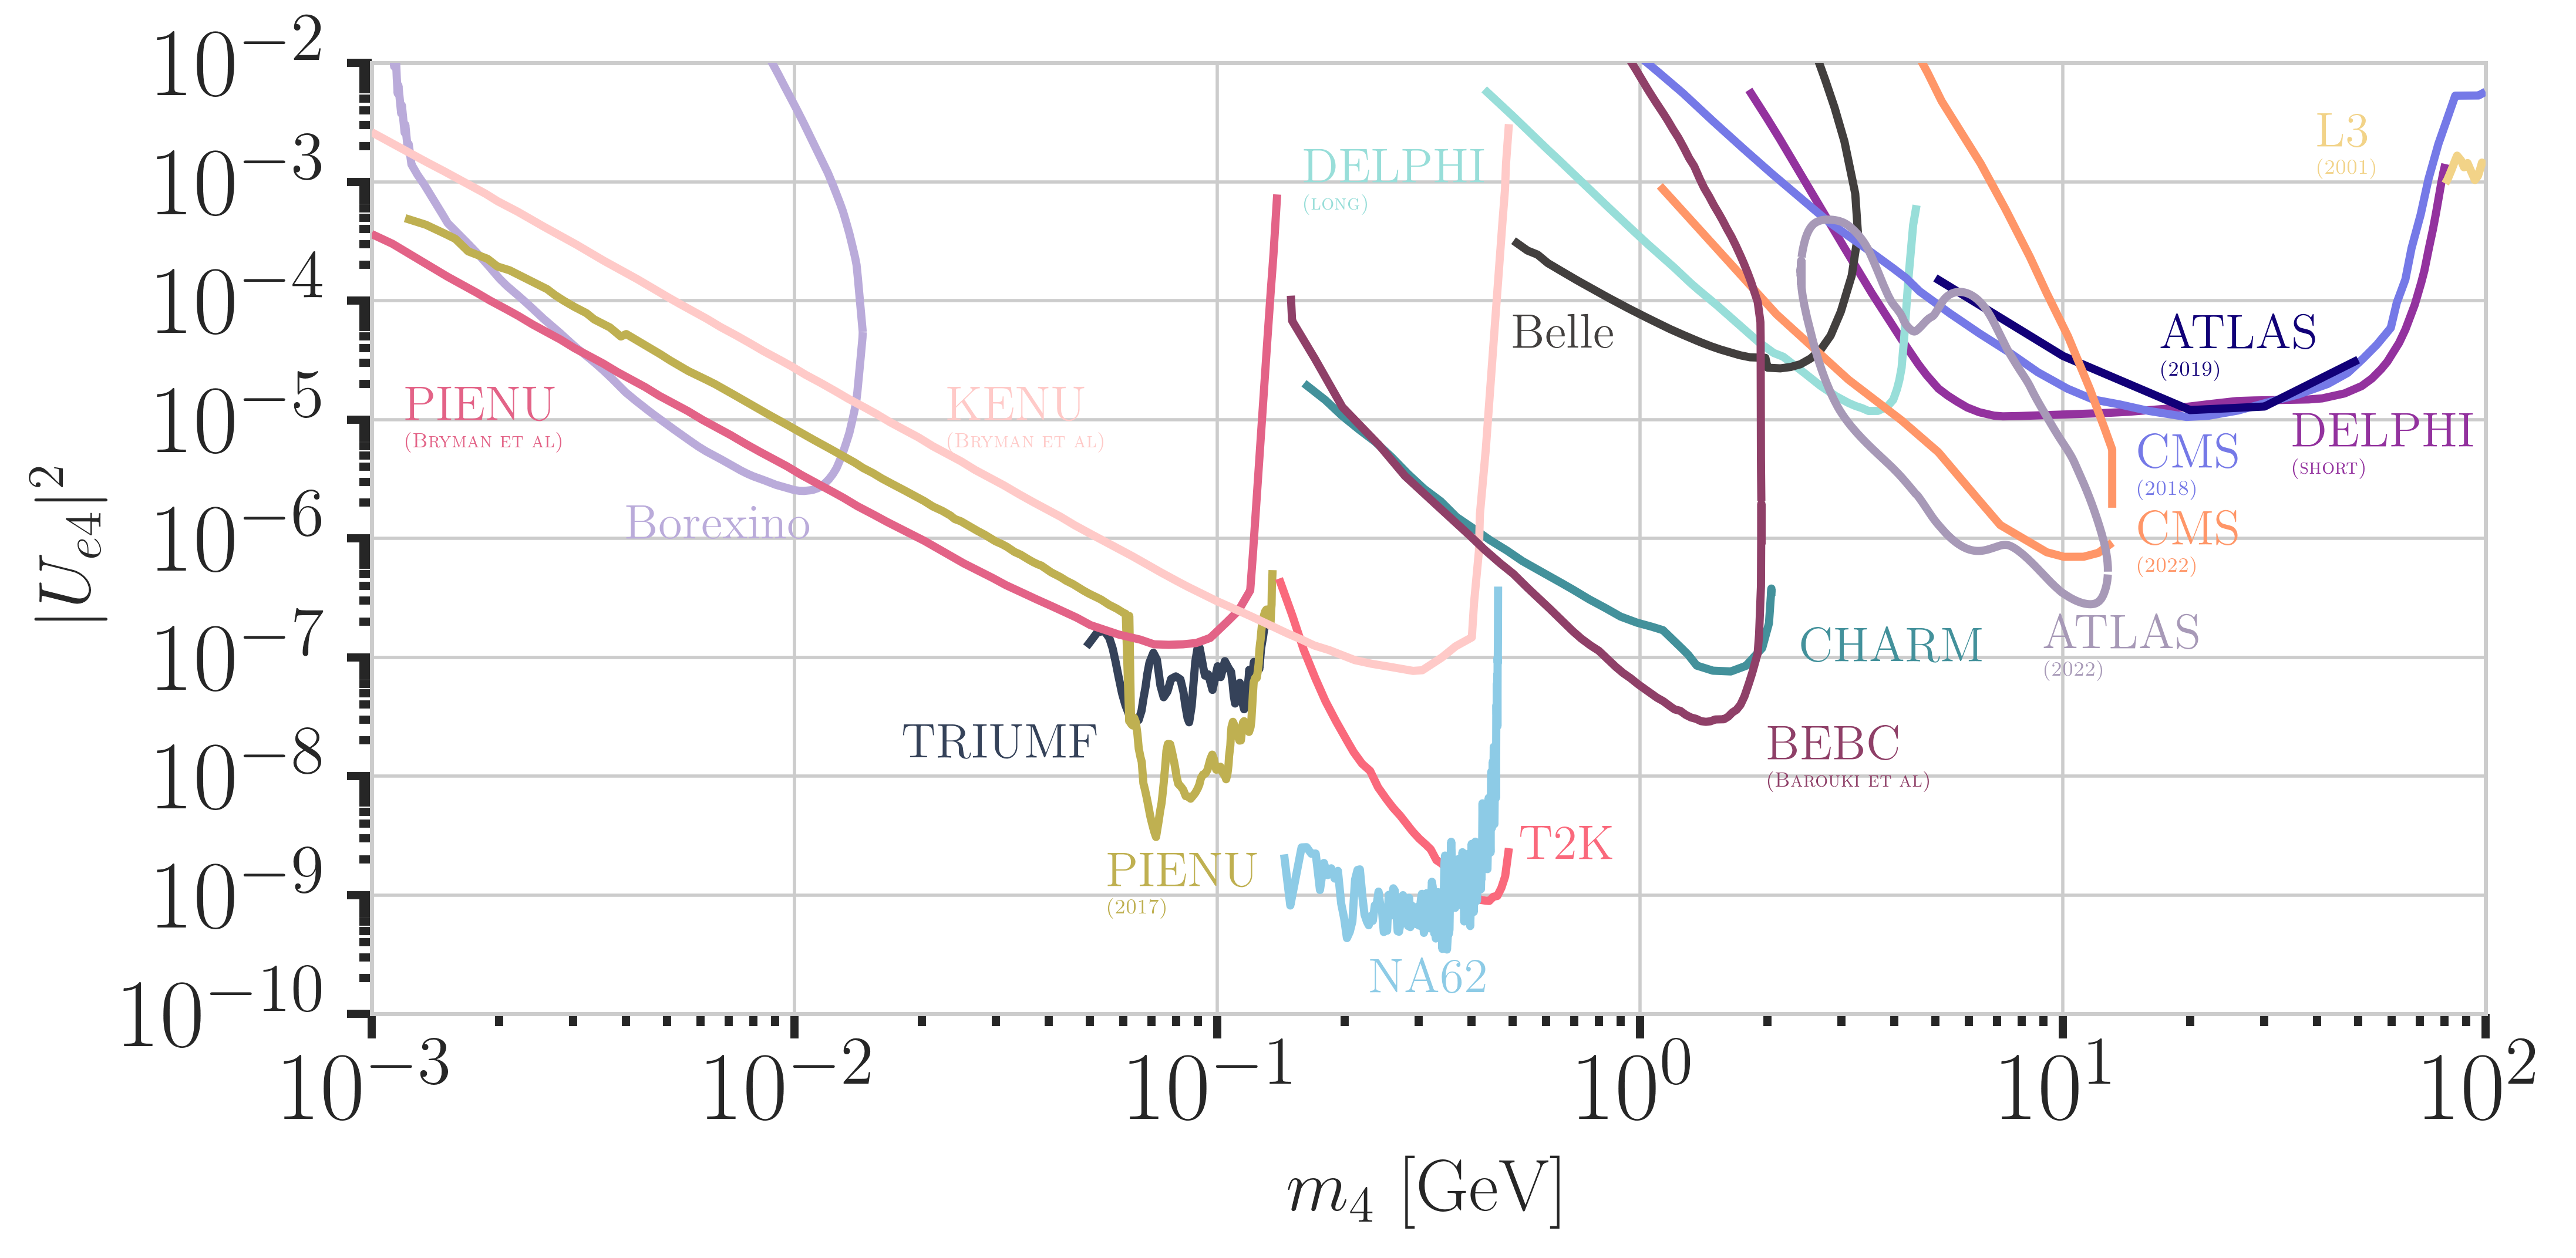
\includegraphics{figures/hnl_simulation/theory/UeN_majorana.png}
      \caption[Current leading $|U_{e4}^2|-m_4$ upper limits]{Current leading $|U_{e4}^2|-m_4$ upper limits from PIENU \cite{pienu_Bryman:2019bjg, PIENU:2017wbj}, BOREXINO \cite{Borexino:2013bot}, KENU \cite{pienu_Bryman:2019bjg}, TRIUMF \cite{triumf_ue4_Britton1992ImprovedSF}, NA62 \cite{NA62:2022pyf}, T2K \cite{T2K:2019jwa}, DELPHI \cite{DELPHI:1996qcc}, BEBC \cite{Barouki:2022bkt}, Belle \cite{Belle:2013ytx}, L3 \cite{L3:2001zfe}, CHARM \cite{CHARM:1983ayi}, ATLAS \cite{ATLAS:2019kpx, atlas_2022_HNL_PhysRevLett.131.061803}, CMS \cite{CMS:2018iaf, CMS:2022fut}, and NuTeV \cite{NuTeV:1999kej}. Modified from \cite{hoster_limitFernandez-Martinez:2023phj}.}
    \labfig{boundsUe}
\end{figure*}

Protons interacting with a target or a beam dump can produce pions, kaons, and heavy-quark hadrons, whose subsequent decays would also produce HNLs. Depending on the HNL lifetime in the specific model, the mass of the HNLs produced in beam dump experiments would be between \SI{1}{\mega\electronvolt} and \SI{4}{\gev} and they could decay at distances across several orders of magnitude, Experiments along the extracted beamline, which are using a spectrometer with particle identification, can search for unique decay signatures at displaced vertices. Example signatures\sidenote{The explicit channels and their decay width calculations used in this thesis are explained in detail in \refsec{custom_leptoninjector}.} are $\nu_4 \rightarrow l_\alpha \pi^+$, $\nu_4 \rightarrow \nu_\alpha l^+_\beta l^-_\beta$, or $\nu_4 \rightarrow \nu_\alpha \pi^0$ (or other neutral mesons) that cannot be explained by SM neutrinos. Here, $\nu_\alpha$ and $l_\alpha$ are the SM neutrino and charged lepton of flavor $\alpha \in \{e,\mu,\tau\}$, defined by which flavor the HNL couples to. $l^-_\beta$/$l^+_\beta$ is a charged lepton/antilepton pair of any flavor $\beta \in \{e,\mu,\tau\}$. Depending on the decay channel, a specific mixing can be probed. The other way of searching for HNLs with these interactions is to look for peaks in the missing mass spectrum, measured around the production vertex at the target, which usually is not possible for beam dumps, as the beam dump region is not calorimetrically instrumented. The HNL searches were pioneered by experiments at extracted beamlines, with \textit{PS191} \sidecite{Bernardi:1985ny} and \textit{CHARM} \sidecite{CHARM:1983ayi} establishing upper limits on \ue4, \um4, and combinations of them, at masses from \SIrange{10}{500}{\mega\electronvolt} at orders of $10^{-3}$ to $10^{-6}$. Since then, there has been and still is a large activity of searches for HNLs at extracted beamlines and at the lower mass end, the strongest bounds on \ue4 are set by \textit{PIENU} \sidecite{pienu_Bryman:2019bjg} at $\sim(10^{-4})$ around \SI{2}{\mega\electronvolt}, and at the higher mass end, the strongest bounds are set by \textit{NA62} \sidecite{NA62:2022pyf}, reaching down to $\sim10^{-9}$ at \SI{0.3}{\gev}. For \um4, the strongest bounds up to \SI{10}{\gev} are set by \textit{PSI} \sidecite{PSI_Daum:1987bg} at $\sim10^{-5}$, and reach down to $\sim(10^{-9})$ at \SI{0.3}{\gev}, by \textit{BNL-E949} \sidecite{BNL_E949:2014gsn}. The current strongest bounds are shown in \reffig{boundsUe} and \reffig{boundsUm}, where bounds from other type of experiments are also presented. Those will be discussed in the following.

Especially noteworthy are the results of analyses probing the mixing with the third lepton generation, \ut4, from \textit{NOMAD} \sidecite{NOMAD:2001eyx} and reinterpretations of the CHARM results and the BEBC results in the context of the mixing \ut4, where the latter places the most stringent limits from $10^{-3}$ to $10^{-6}$ in the \SIrange{0.1}{2}{\gev} range \sidecite{Orloff:2002de, Boiarska:2021yho, Barouki:2022bkt}. In \reffig{boundsUt} the current strongest bounds on \ut4 are shown.


\subsubsection{Collider Searches}

\begin{figure*}[t]
    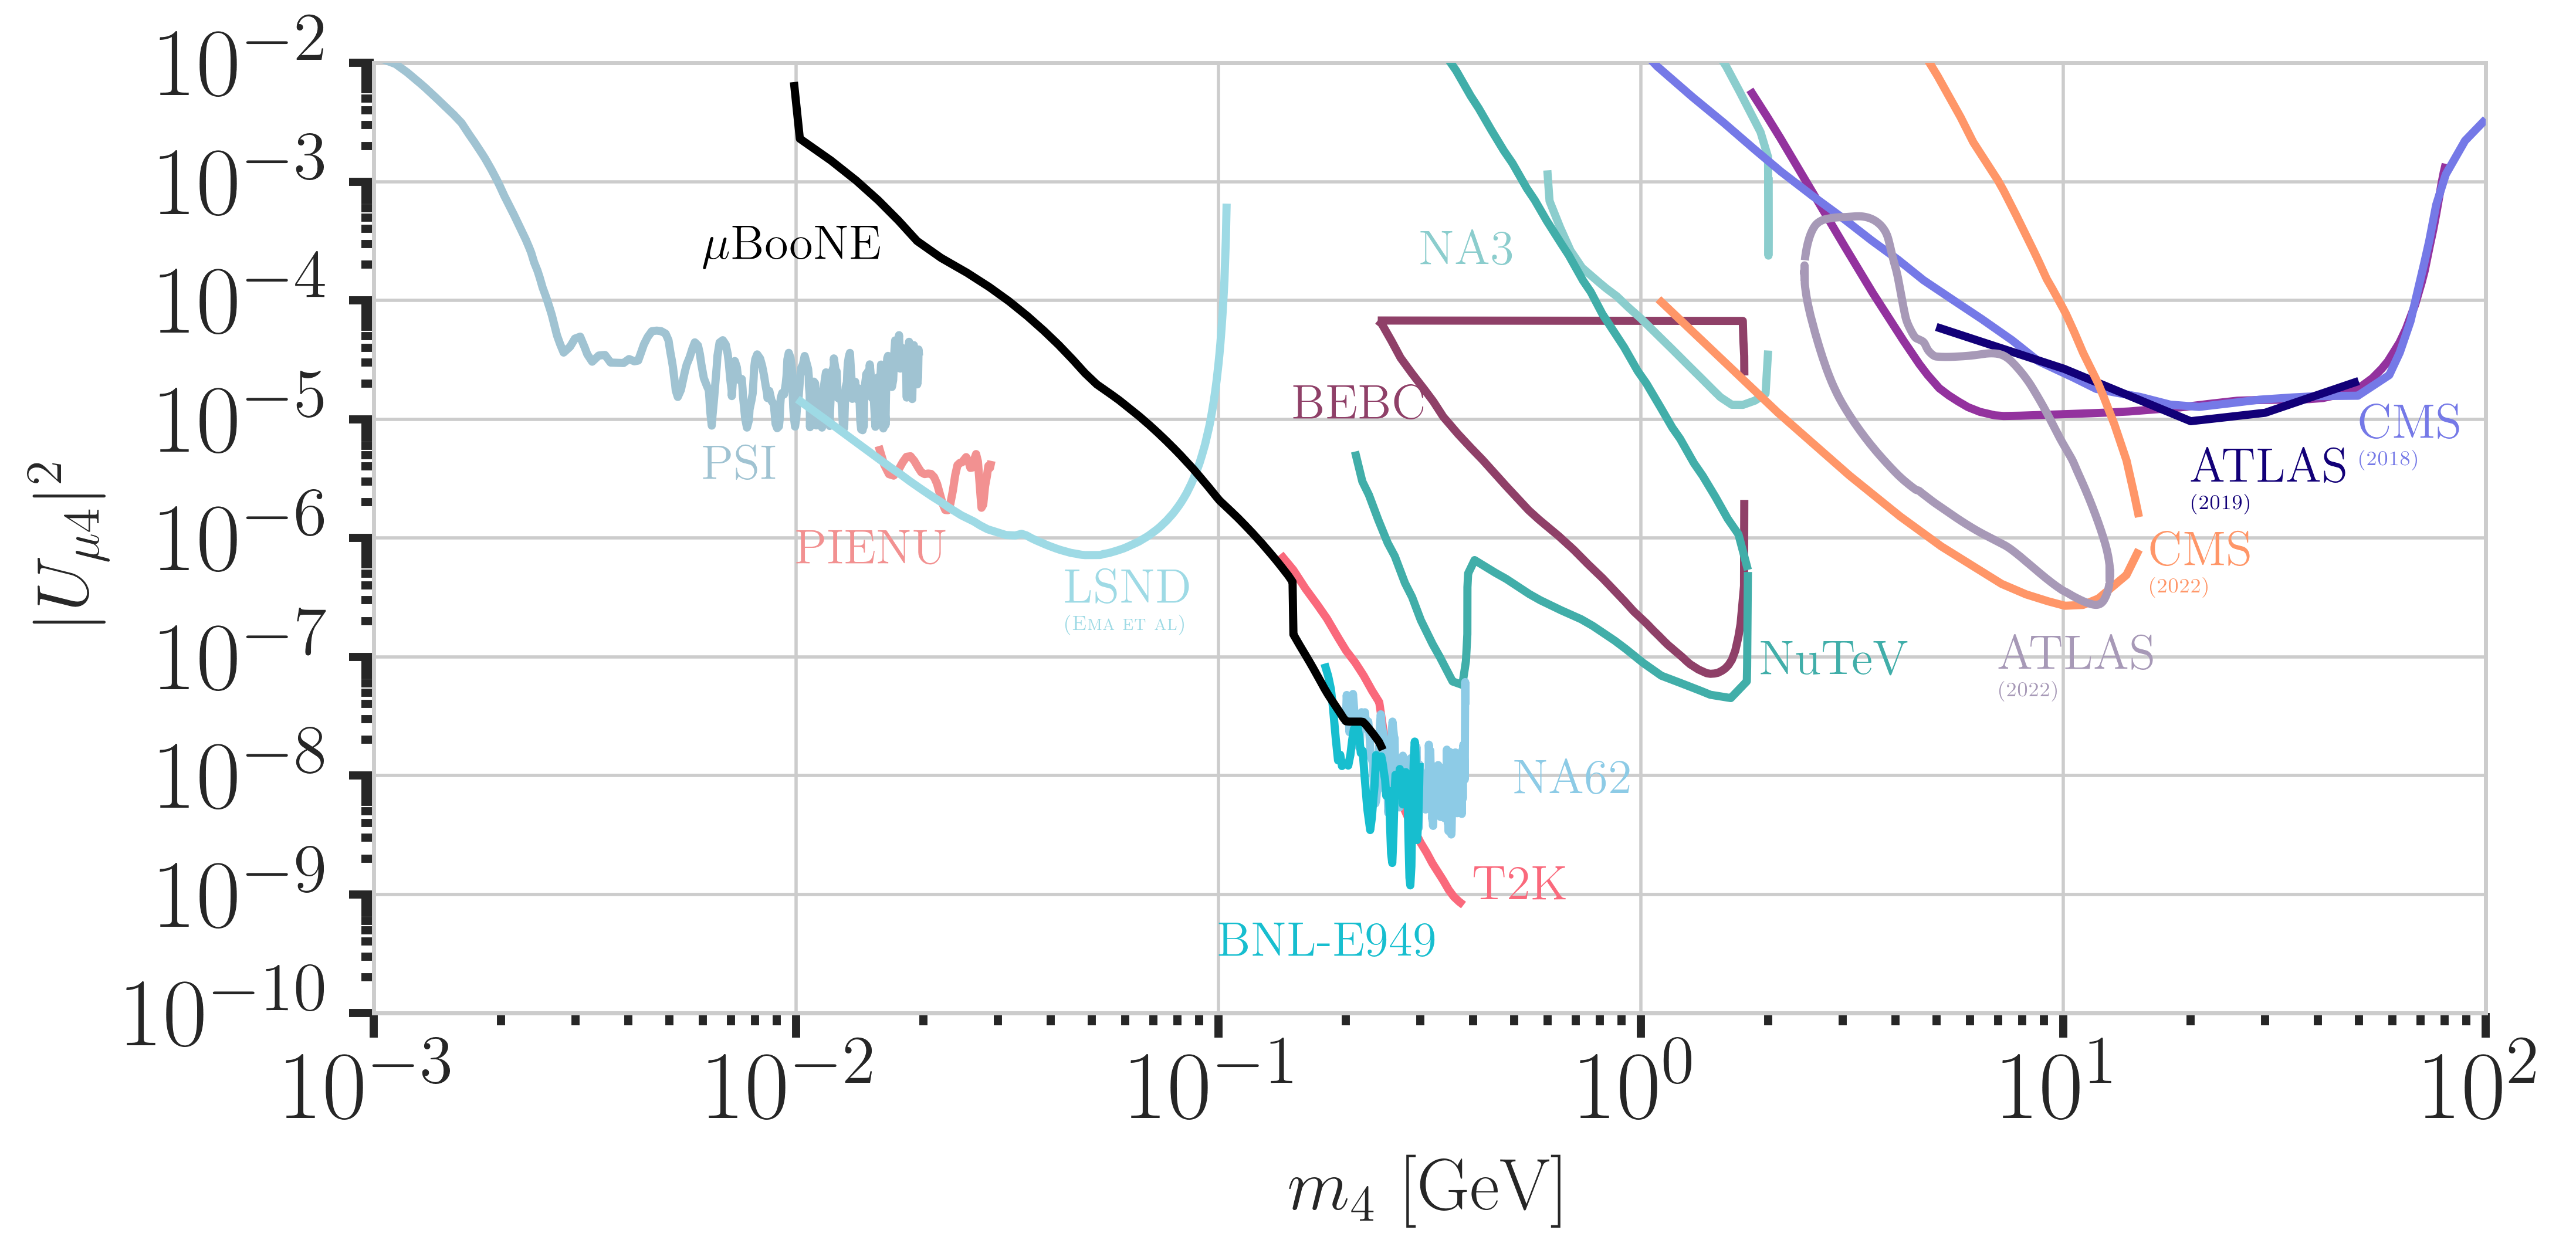
\includegraphics{figures/hnl_simulation/theory/UmuN_majorana.png}
      \caption[Current leading $|U_{\mu4}^2|-m_4$ upper limits]{Current leading $|U_{\mu4}^2|-m_4$ upper limits from PSI \cite{PSI_Daum:1987bg}, $\mu$BooNE \cite{MicroBooNE:2023eef}, PIENU \cite{pienu_Bryman:2019bjg}, LSND \cite{lsnd_Ema:2023buz}, BNL-E949 \cite{BNL_E949:2014gsn}, NA62 \cite{NA62:2022pyf}, T2K \cite{T2K:2019jwa}, BEBC \cite{BEBC_OG_COOPERSARKAR1985207},
      ATLAS \cite{ATLAS:2019kpx, atlas_2022_HNL_PhysRevLett.131.061803}, CMS \cite{CMS:2018iaf, CMS:2022fut}, NuTeV \cite{NuTeV:1999kej}, and NA3 \cite{NA3:1986ahv}. Modified from \cite{hoster_limitFernandez-Martinez:2023phj}.}
    \labfig{boundsUm}
\end{figure*}


So far, collider searches have been conducted at the \textit{large electron positron collider (LEP)} and at the \textit{large hadron collider (LHC)} in proton-proton mode. Strongest results are from the \textit{ATLAS} and \textit{CMS} experiments, which are nearly hermetic, general purpose detectors around the interaction point, and from the \textit{DELPHI} and the \textit{LHCb} experiments, which are forward detectors that can be used to search for new particles in decays of heavy particles produced. In the minimal model, HNLs in the \si{\gev} mass range can be produced through mass mixing in decays of heavy mesons, tau leptons, Z/W bosons, H bosons, or top quarks originating from the collisions. Depending on the dirac or majorana nature of the HNL, they can decay to lepton number conserving or lepton number violating channels.

Using prompt and displaced decays of the HNL, both ATLAS and CMS have set constraints on \ue4 and \um4 at the level of $10^{-4}$ to $10^{-6}$ in the mass range between \SIrange{1}{100}{\gev} \sidecite{ATLAS:2019kpx, atlas_2022_HNL_PhysRevLett.131.061803, CMS:2018iaf, CMS:2022fut}. The LHCb experiment has HNL search results at HNL masses below and above the W boson mass, where the low mass searches are using the decay channel $B^- \rightarrow \pi^+ \mu^- \mu^-$, setting limits at the $10^{-3}$ level for \um4 in the mass range of \SIrange{0.5}{3.5}{\gev} \sidecite{Shuve:2016muy}. At high masses, the $W^+ \rightarrow \mu^- \mu^\pm$jet channel is used to set limits at the order of $10^{-3}$ to $10^{-2}$ for \um4 in the mass range of \SIrange{5}{50}{\gev} in the LNC channel and at the order of $10^{-4}$ to $10^{-3}$ in the LNV channel \sidecite{LHCb:2020wxx}. Using hadronic $Z^0$ decays, searches for short- and long-lived HNLs have been conducted with the \textit{DELPHI} detector setting upper limits of the order of $10^{-5}$ for mixing to any SM flavor in the mass range from \SIrange{3.5}{50}{\gev} \sidecite{DELPHI:1996qcc}. 


\subsubsection{Nuclear Decays Measurements}

\begin{figure*}[t]
    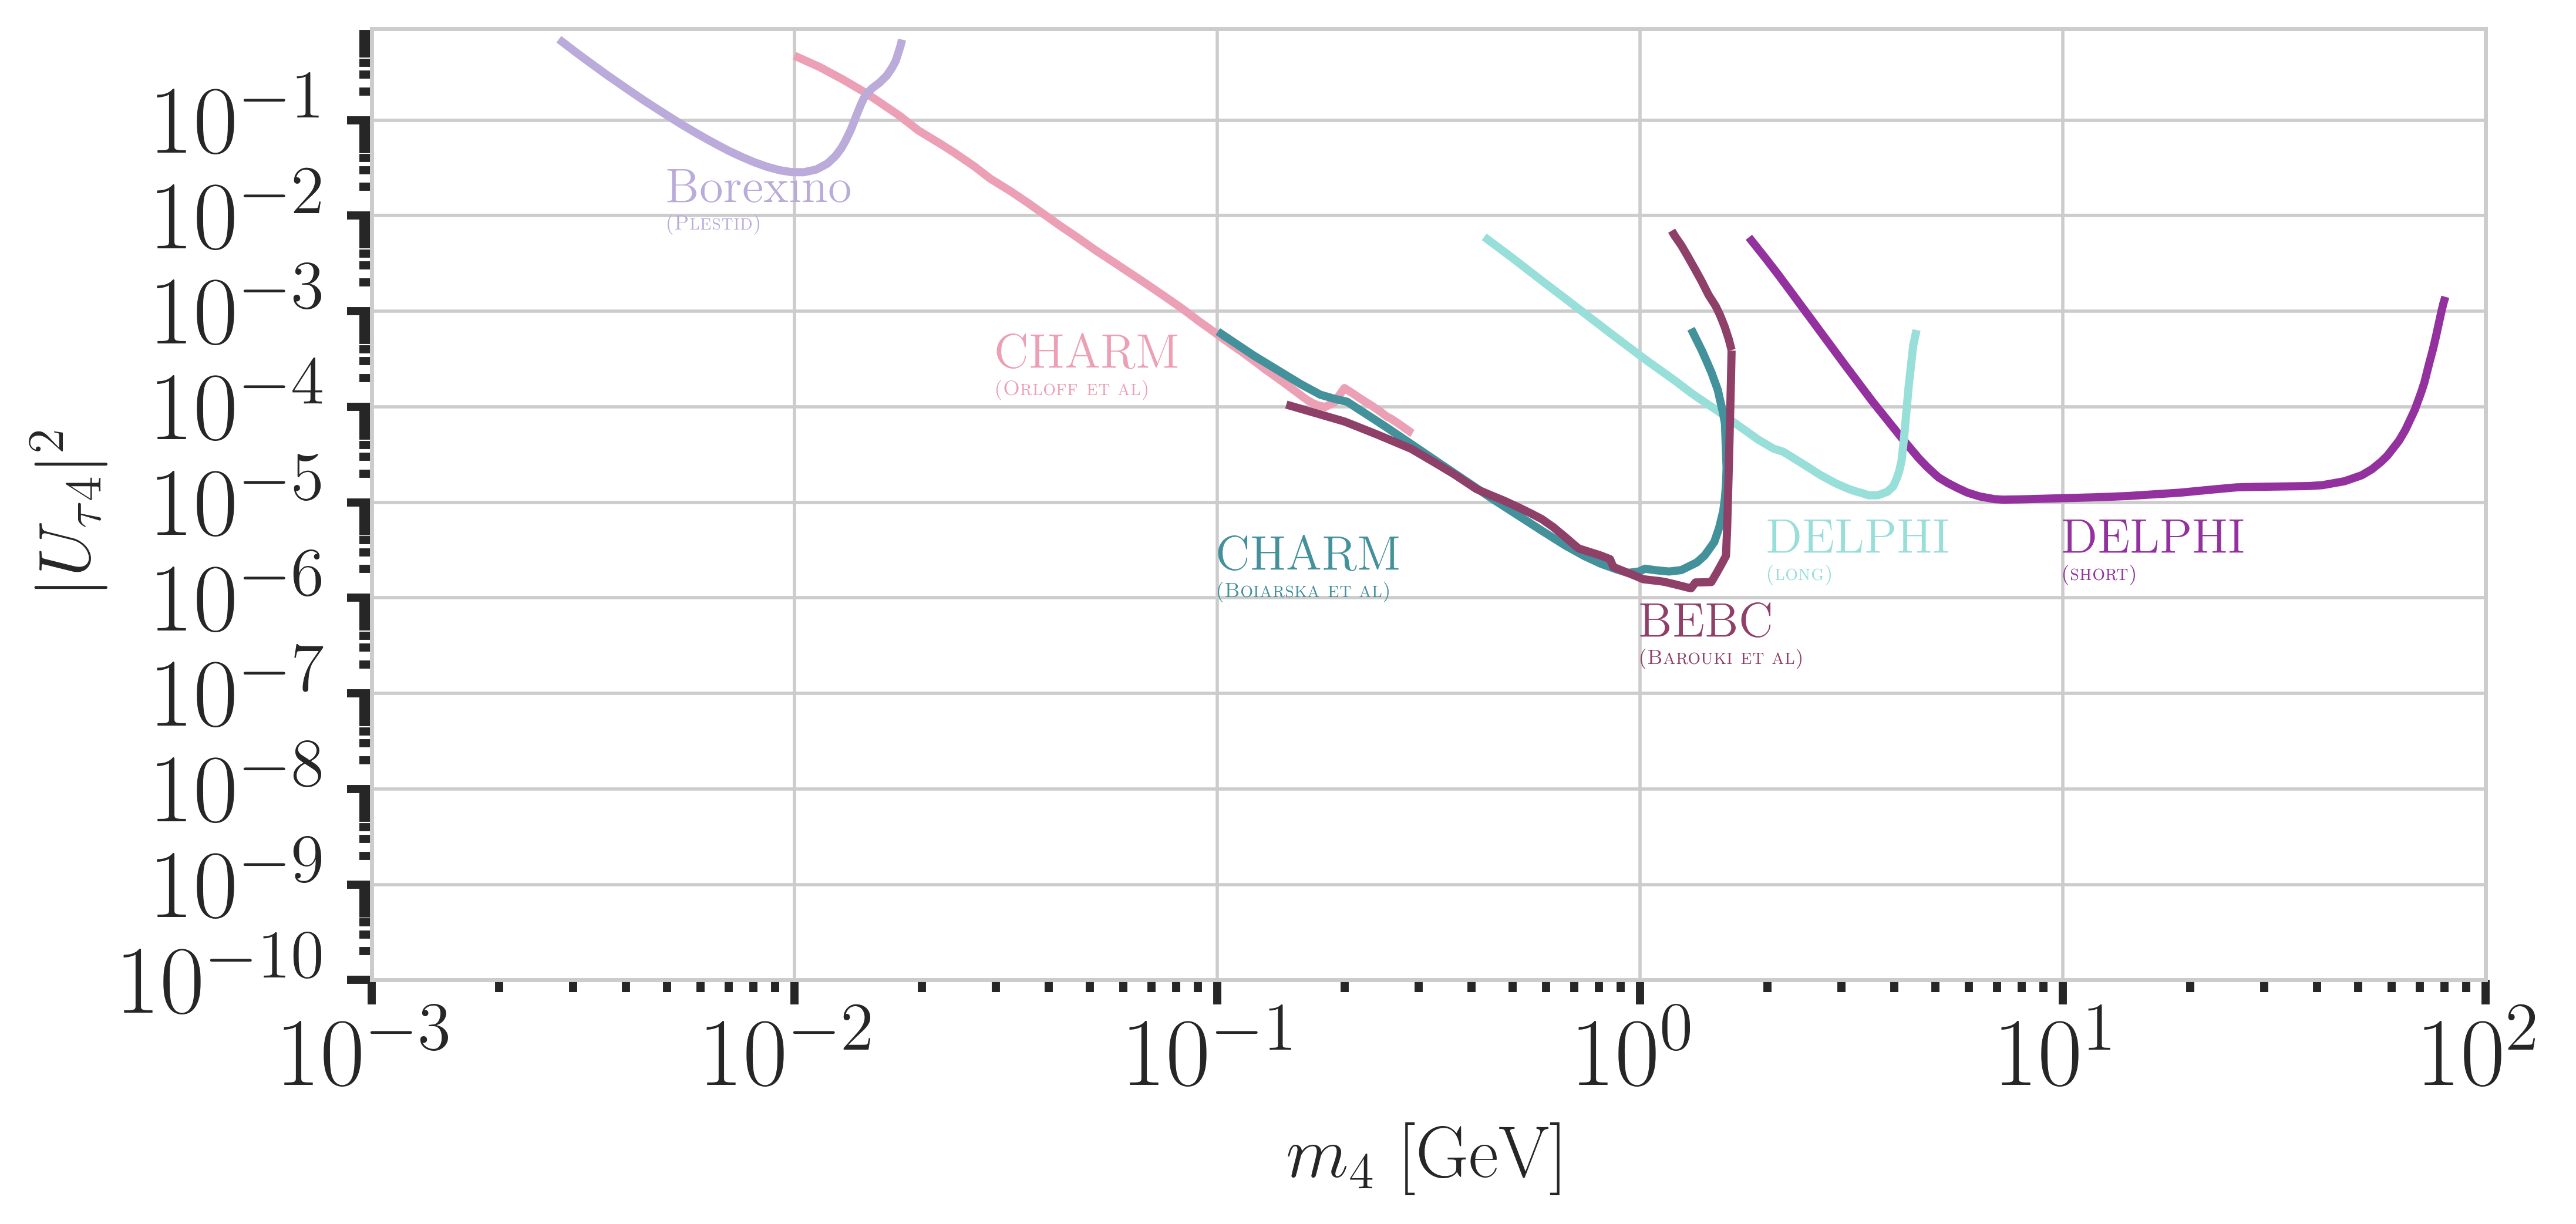
\includegraphics{figures/hnl_simulation/theory/UtauN_majorana.png}
      \caption[Current leading $|U_{\tau4}^2|-m_4$ upper limits]{Current leading $|U_{\tau4}^2|-m_4$ upper limits from BOREXINO \cite{Plestid:2020vqf}, CHARM \cite{Orloff:2002de, Boiarska:2021yho}, DELPHI \cite{DELPHI:1996qcc}, and BEBC \cite{Barouki:2022bkt}. Modified from \cite{hoster_limitFernandez-Martinez:2023phj}.}
    \labfig{boundsUt}
\end{figure*}

A novel approach of searching for irregularities in energy-momentum conservation measurements in nuclear reactions might be a viable way of searching for HNLs, as they could be interpreted as constraints on \ue4 and $m_4$.

Kinks in \textbf{beta decay} spectra would show up at $Q-m_4c^2$, where the HNL mass, $m_4$, can be measured between the lower energy detection threshold and the energy released in the decay, which is called $Q$ value. Analyses using the tritium decay, with $Q=\SI{18.6}{\kilo\electronvolt}$, are planned in \textit{KATRIN} \sidecite{KATRIN:2001ttj} and \textit{TRISTAN} \sidecite{Mertens_2019} in the \SIrange{1}{18}{\kilo\electronvolt} range. Their projected statistical limits are around $10^{-7}$ for \ue4, but will require further detector upgrades \cite{Mertens_2019}. A first result from KATRIN measurements during commissioning sets limits at the order of $10^{-2}$ to $10^{-3}$ in the mass range of \SIrange{0.1}{1.6}{\kilo\electronvolt} \sidecite{KATRIN:2022spi}. \textit{DUNE} is planning to measure the ionization charge of atmospheric argon decays, with $Q=\SI{565}{\kilo\electronvolt}$, to probe \ue4 at in the \SIrange{20}{450}{\kilo\electronvolt} mass range. The projected sensitivity is at the $10^{-5}$ level, and might improve to $10^{-7}$ with additional detector improvements \sidecite{DUNE:2020ypp}.

To test for the existence of HNLs using \textbf{electron capture} measurements, total energy-momentum reconstruction of all non-neutrino final states is needed. Electron capture is a pure two-body decay process, where the recoiling atom and the electron neutrino are the only final state particles, but additional energy is carried away by the de-excitation x-ray or auger electron. The energy-momentum conservation can be probed by measuring the atom and the associated de-excitation products. The mixing \ue4 can be probed by looking for a separated non-zero missing mass peak. The \textit{BeEST} experiment has set limits at the $10^{-4}$ level in the \SIrange{100}{850}{\kilo\electronvolt} mass range, using berillium-7, which has a $Q$ value of \SI{862}{\kilo\electronvolt}. After planned upgrades to the experiment, the sensitivity is expected to improve to the $10^{-7}$ level \sidecite{BeEST_Friedrich:2020nze}.

\textbf{Reactor searches} up to \SI{12}{\mega\electronvolt} in mass are possible at short baseline experiments using commercial or research reactors, which are a strong source of electron antineutrinos and could therefore also produce HNLs if \ue4 is non-zero. Visible decay channels at these energies are $\nu_4 \rightarrow \nu_e e^+ e^-$, $\nu_4 \rightarrow \nu \gamma$, and $\nu_4 \rightarrow \nu \gamma \gamma$, where the first dominates. The first analysis in this field, reports limits at the $10^{-4}$ level in the \SIrange{2}{7}{\mega\electronvolt} mass range \sidecite{de59e8a4525048378bfd5f3973e2d6ad}.


\subsubsection{Atmospheric and Solar Neutrinos}

Natural sources of neutrinos are provided up to \SI{20}{\mega\electronvolt} by the sun and up to 100s of \si{\gev} by neutrino production in the atmosphere. Both fluxes contain all flavors of neutrinos, due to mixing and oscillations, and can therefore be used to directly probe the mixings with $\nu_e$, $\nu_\mu$, and $\nu_\tau$. Depending on the HNL mass and the strength of the mixing, which both govern the decay length, different signatures can be used to experimentally access large regions of the HNL parameter space. The strength of the mixing determines the total rate of HNL events, which is additionally affected by whether solely the minimal mass mixing is assumed, or also more complicated mixing scenarios, like the dipole portal, are considered.

So far, only very few analyses exist, which are performed by the experimental collaborations themselves. Several external theoretical groups have predicted the expected sensitivities to HNLs, produced from solar or atmospheric neutrinos, based on various coupling scenarios and decay lengths. A selection of the potential analyses will be discussed in the following.

For very long-lived particles, \textbf{production inside the sun} can be used as a source to search for HNLs in detectors on earth. This will only allow production through non-zero \ue4, because the initial solar neutrino flux is only $\nu_e$. By searching for HNL decays to a SM neutrino and an electron positron pair $\nu_4 \rightarrow \nu_e e^+ e^-$ and comparing to the expected inter planetery positron flux, \textit{Borexino} has placed the strongest limits on the mixing \ue4 at the order of $10^{-5}$ in the few \si{\mega\electronvolt} mass range \sidecite{Borexino:2013bot}.

For HNL decay length scales of the order of the Earth's diameter, HNL \textbf{up-scattering outside the detector} is possible, where a neutrino from the solar or the atmospheric neutrino flux scatters in the Earth and transfers some kinetic energy to the HNL, which can then later decay inside the detector. For HNL masses below \SI{18}{\mega\electronvolt} produced from solar neutrinos, limits were derived using the Borexino data for purely tau coupling through mass mixing \sidecite{Plestid:2020vqf} and for all flavor coupling through the dipole portal \sidecite{Plestid:2020ssy}. At similar decay length scales, the HNL could also be produced directly in the atmosphere, but neither this channel, nor the production anywhere in the Earth from atmospheric neutrinos has been investigated yet.

If the HNL decay lengths are sufficiently short, \textbf{production and decay in the detector} can happen and the observation of two vertices could be used to constrain the mixing parameters. In principle, this could be possible with any neutrino flavor produced in the sun or the atmosphere, but so far only theoretical studies have been performed for mass-mixing and dipole-portal couplings for the atmospheric neutrino detectors IceCube \sidecite{Coloma:2017ppo,Coloma:2019qqj} and \textit{Super-K}, \textit{Hyper-K}, and Dune \sidecite{Atkinson:2021rnp, Coloma:2020lgy}. Due to the high complexity of these experiments, several simplified assumptions were made in the studies, which might not hold in reality, and the results should be taken with caution. For reliable sensitivity estimates and limits the collaborations should perform their own analyses.


\section{Atmospheric Neutrinos as Source of Heavy Neutral Leptons} \labsec{hnl_theory}

This work focuses on the search for HNLs using atmospheric neutrinos as source for the production and decay inside the IceCube detector. The following sections will give a brief overview of the production of neutrinos in the atmosphere and the oscillations they undergo, before discussing the expected signatures of HNLs in the detector, where they are produced from the incoming neutrinos and subsequently decay.


\subsection{Production of Neutrinos in the Atmosphere}

The analysis performed in this work is based on the sample of neutrinos observed in IceCube DeepCore at energies below \SI{100}{\gev}. At these energies, the flux exclusively originates in the Earth's atmosphere. Highly relativistic cosmic rays (protons and heavier nuclei \sidecite{PhysRevD.98.030001}) interact in the upper atmosphere, producing showers of secondary particles. Neutrinos are produced in decays of charged pions and kaons ($\pi$ and $K$ mesons) present in those showers, where the dominant contribution comes from the decay chain
\begin{equation}
    \begin{split}   
        \pi^\pm &\rightarrow \mu^\pm + \nu_\mu(\bar{\nu}_\mu)\;, \\
        \mu^\pm &\rightarrow e^\pm + \bar{\nu}_\mu(\nu_\mu) + \nu_e(\bar{\nu}_e)
        \;,
    \end{split}
    \labeq{pion_decay}
\end{equation}
where muon neutrinos $\nu_\mu$ and muons $\mu^\pm$ are produced in the first decay and both electron and muon neutrinos $\nu_{e/\mu}$ are produced in the second decay. Atmospheric muons, which are also produced in these decays, are the main background component for IceCube DeepCore analyses.

\begin{figure}
    \centering
    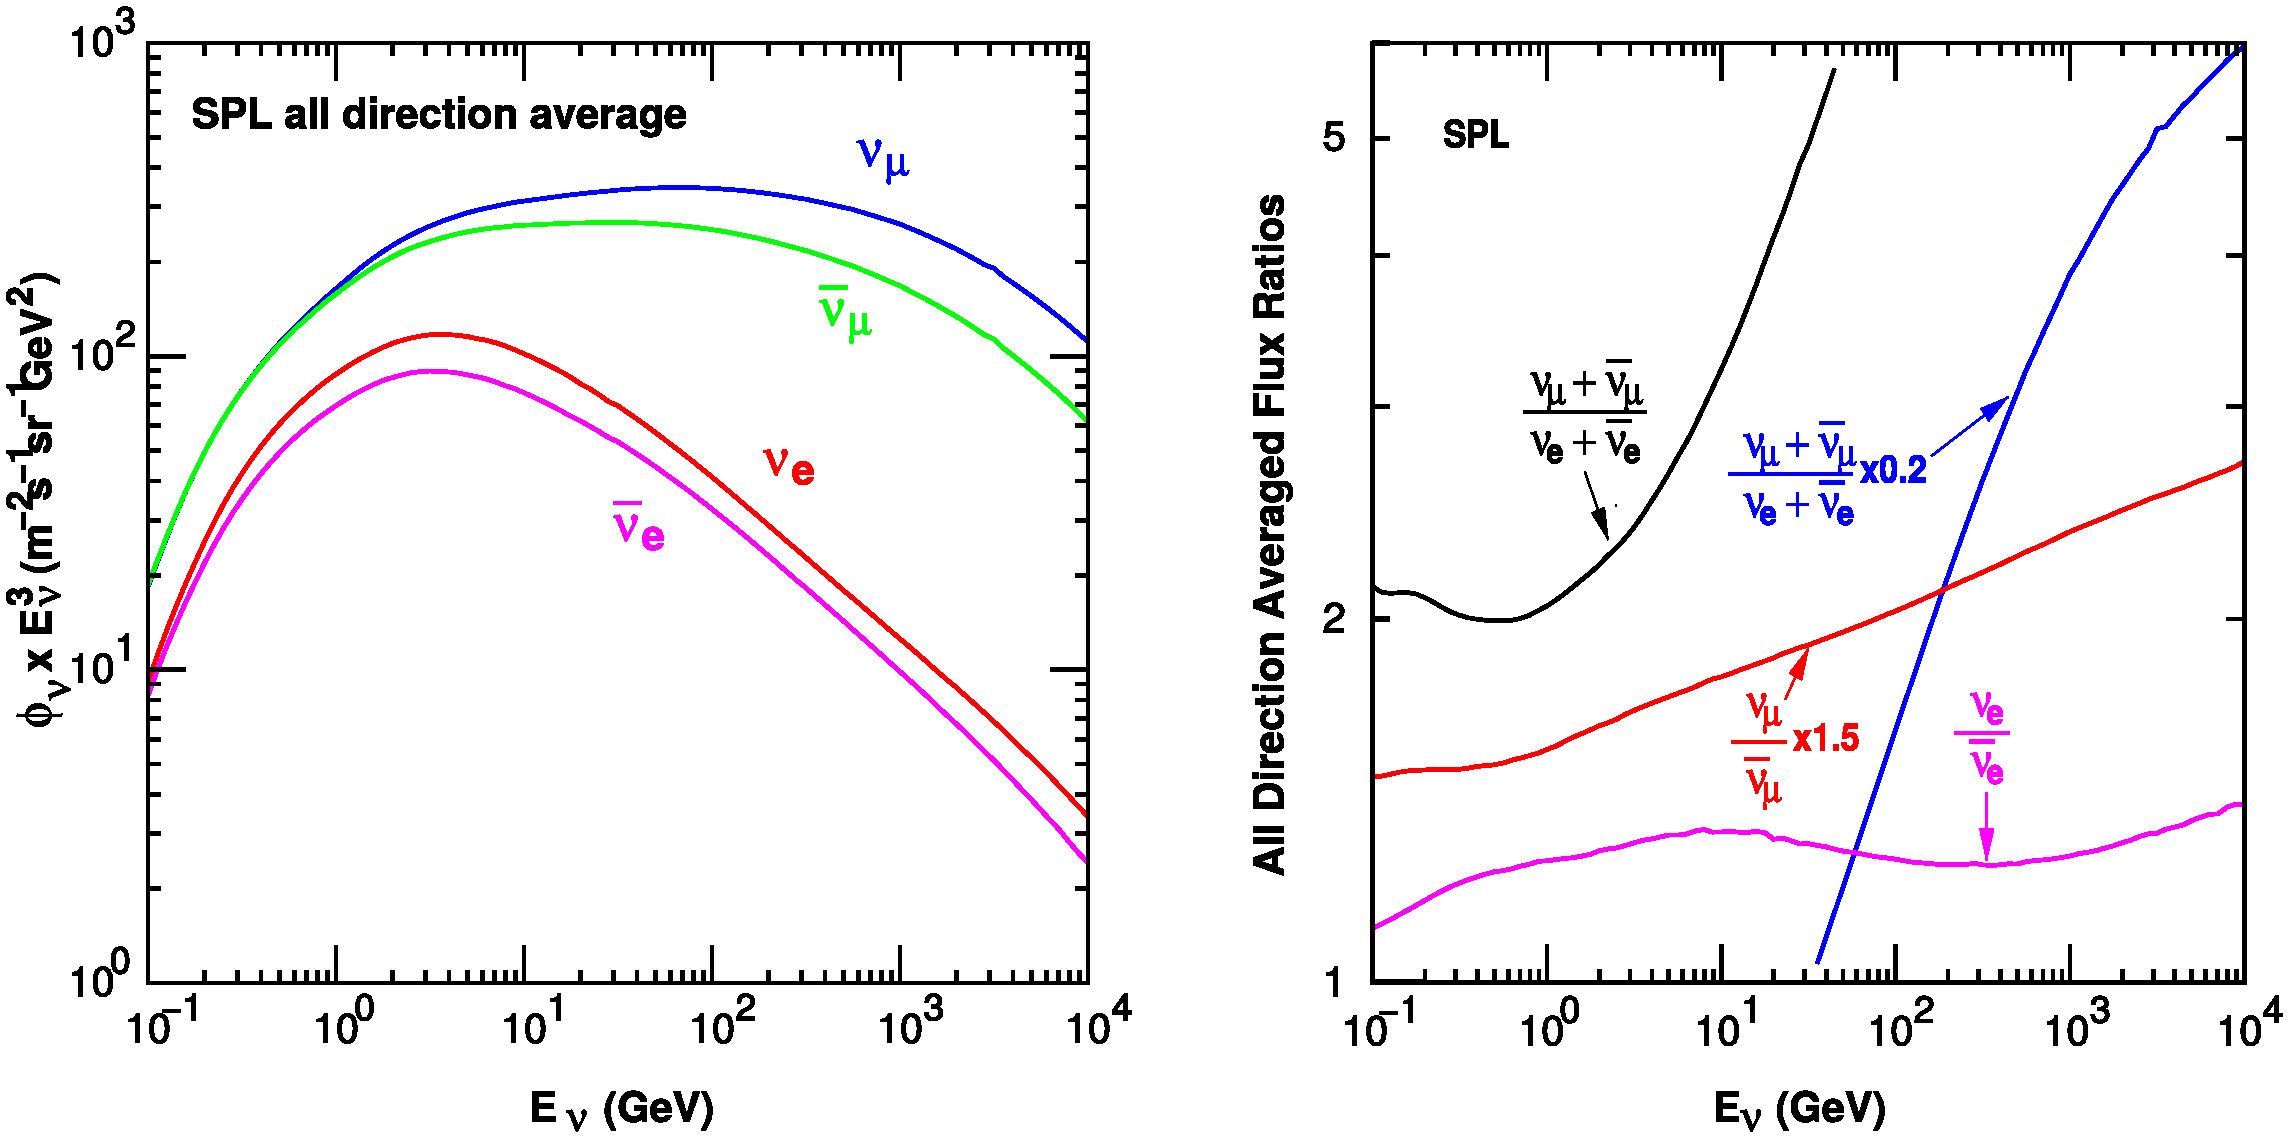
\includegraphics[width=1.0\textwidth]{figures/neutrinos_properties/Honda_alldir-spl_copy.pdf}
    \caption[Atmospheric neutrino fluxes]{The atmospheric fluxes of different neutrino flavors as a function of energy (left) and the ratios between muon neutrinos and electron neutrinos as well as the ratios between neutrinos and antineutrinos for both those flavors (right). Results from the calculations performed for the geographic South Pole, taken from \cite{PhysRevD.92.023004_Honda_Flux}.}
    \labfig{honda_flux}
\end{figure}

The different atmospheric flux components are shown in \reffig{honda_flux} (left), for a much broader energy range than relevant for this work. Both neutrinos and antineutrino fluxes are shown for electron  and muon neutrinos and all fluxes are the directionally averaged expectation calculated at the South Pole. Muon neutrinos are dominating the flux and from \refeq{pion_decay} the naive assumption would be that the ratio between muon and electron neutrinos is $(\nu_\mu+\bar{\nu}_\mu)/(\nu_e+\bar{\nu}_e)=2$. This is roughly true at energies below \SI{1}{\gev}, where all muons decay in flight, but at larger energies muons can reach the detector before decaying, which increases the ratio to approximately 10:1 at around \SI{100}{\gev}. Additionally, kaon decays start to contribute which also increases the number of muons and muon neutrinos. The increasing ratio can be seen in \reffig{honda_flux} (right), which also shows the ratio between neutrinos and antineutrinos for both flavors.

Charged mesons heavier than the tau can also be produced in cosmic ray interactions. Their decays to tau neutrinos or direct production of taus in cosmic ray interactions lead to the production of tau neutrinos. At the energies relevant for this work however, the resulting tau neutrino flux is negligible as compared to the muon neutrino flux \sidecite{2015EPJWC..9908001F_lepton_fluxes} and is not considered in the analysis. This is because both charged mesons and tau particles are much heavier than pions and kaons and therefore their production is suppressed at high energies.


\subsection{Neutrino Oscillations} \labsec{neutrino_oscillations}

Describing neutrinos in their mass state as introduced in \refsec{neutrino_mass_mixing} is crucial to understanding their propagation through space and time and to explaining neutrino oscillations. Oscillations mean that a neutrino changes from its initial flavor, that it was produced with, to another flavor and back after traveling a certain distance.

The neutrino propagation in vacuum can be expressed by applying a plane wave approach, where the mass eigenstates evolve as
\begin{equation}
    \ket{\nu_k(t)} = e^{-iE_kt/\hbar}\ket{\nu_k}
    \;.
    \labeq{flavor_time_evol}
\end{equation}
The energy of the mass eigenstate $\ket{\nu_k}$ is $E_k=\sqrt{\vec{p}^2c^2+m_k^2c^4}$, with momentum $\vec{p}$ and mass $m_k$, $\hbar$ is the reduced Planck constant, and c is the speed of light in vacuum. A neutrino is produced as a flavor eigenstate $\ket{\nu_\alpha}$ in a CC weak interaction, but its propagation happens as the individual mass states it is composed of. The probability of finding the neutrino with initial flavor $\ket{\nu_\alpha}$ in the flavor state $\ket{\nu_\beta}$ after the time $t$ is calculated as
\begin{equation}
    P_{\nu_\alpha \rightarrow \nu_\beta}(t)
    =
    \big|\braket{\nu_\beta|\nu_\alpha(t)}\big|^2
    \;,
    \labeq{fermis_golden_rule}
\end{equation}
by applying Fermi's Golden Rule \sidecite{1927RSPSA.114..243D}, which defines the transition rate from one eigenstate to another by the strength of the coupling between them. This coupling strength is the square of the matrix element and using the fact that the mixing matrix is unitary ($U^{-1}=U^\dagger$) to describe the mass eigenstates as flavor eigenstates, we find the time evolution of the flavor state $\ket{\nu_\alpha(t)}$, which can be inserted into \refeq{fermis_golden_rule} to find the probability as
\begin{equation}
    P_{\nu_\alpha \rightarrow \nu_\beta}(t)
    =
    \sum_{j,k}U^*_{\beta j}U_{\alpha j}U_{\beta k}U^*_{\alpha k}e^{-i(E_k-E_j)t/\hbar}
    \;.
    \labeq{probability_raw}
\end{equation}
The indices $j$ and $k$ run over the mass eigenstates.

We can approximate the energy as
\begin{equation}
    E_k \approx E+\frac{c^4m^2_k}{2E} \hspace{0.25cm} \longrightarrow \hspace{0.25cm} E_k-E_j \approx \frac{c^4\Delta m^2_{kj}}{2E}
    \;,
\end{equation}
for very small masses compared to the kinetic energy $E\gg m_kc^2$. Here, $\Delta m^2_{kj}=m^2_k-m^2_j$ is the mass-squared splitting between states $k$ and $j$, and $E$ is the energy of the wavepacket to be detected (flavor eigenstate). Replacing the time in \refeq{probability_raw} by the distance traveled by relativistic neutrinos $t\approx L/c$ we get
\begin{equation}
    \begin{split}
        P_{\nu_\alpha \rightarrow \nu_\beta}(t)
        = 
        \delta_{\alpha \beta}
        -
        4\sum_{j>k}&\textbf{Re}(U^*_{\beta j}U_{\alpha j}U_{\beta k}U^*_{\alpha k})\textrm{sin}^2\Big( \frac{c^3\Delta m^2_{kj}}{4E\hbar}L \Big) \\
        +
        2\sum_{j>k}&\textbf{Im}(U^*_{\beta j}U_{\alpha j}U_{\beta k}U^*_{\alpha k})\textrm{sin}^2\Big( \frac{c^3\Delta m^2_{kj}}{4E\hbar}L \Big)
        \;,
    \end{split}
    \labeq{probability_detailed}
\end{equation}
which is called the survival probability if $\alpha=\beta$, and the transition probability if $\alpha\neq\beta$. Once again, this probability is only non-zero if there are neutrino mass eigenstates with masses greater than zero. Additionally, there must be a mass-squared difference $\Delta m^2$ and non-zero mixing between the states. Since we assumed propagation in vacuum in \refeq{flavor_time_evol}, the transition and survival probabilities correspond to vacuum mixing.

{\renewcommand{\arraystretch}{0.7}
\begin{margintable}[3cm]
    \footnotesize
    \begin{tabular}{ cc }
    \hline\hline    
    Parameter & Global Fit \\
    \hline\hline    
    $\theta_{12}$ [\si{\degree}] & $33.41^{+0.75}_{-0.72}$ \\
    $\theta_{13}$ [\si{\degree}] & $8.54^{+0.11}_{-0.12}$ \\
    $\theta_{23}$ [\si{\degree}] & $49.1^{+1.0}_{-1.3}$ \\
    \hline
    $\Delta m^2_{21}$ [$10^{-5}$\si{\electronvolt^2}] & $7.41^{+0.21}_{-0.20}$ \\
    $\Delta m^2_{31}$ [$10^{-3}$\si{\electronvolt^2}] & $2.511^{+0.028}_{-0.027}$ \\
    \hline
    $\delta_{CP}$ [\si{\degree}] & $197^{+42}_{-25}$ \\
    \hline
    \end{tabular}
\caption[Global fit neutrino mixing parameter results]{Results from the latest global fit of neutrino mixing parameters from \cite{nufit_5.2}.}
\labtab{nufit_5.2}
\end{margintable}
}

The mixing matrix can be parameterized as \sidecite{PhysRevD.98.030001}
\begin{equation}
    U=\left( 
    \begin{matrix}
        1 & 0 & 0 \\
        0 & c_{23}  & s_{23} \\
        0 & -s_{23} & c_{23} 
    \end{matrix}
    \right) 
    \left( 
    \begin{matrix}
        c_{13} & 0 & s_{13}e^{-i\delta_{CP}} \\
        0 & 1 & 0\\
        -s_{13} e^{i\delta_{CP}} & 0 & c_{13}
    \end{matrix}
    \right) 
    \left( 
    \begin{matrix}
        c_{12} & s_{12} & 0 \\
        -s_{12} & c_{12} & 0\\
        0 & 0 & 1
    \end{matrix} 
    \right)  
    \;,
    \labeq{parameterized_PMNS_matrix}
\end{equation}
where $c_{ij}=\cos\theta_{ij}$ and $s_{ij}=\sin\theta_{ij}$ are cosine and sine of the mixing angle $\theta_{ij}$, that defines the strength of the mixing between the mass eigenstates $i$ and $j$, and $\delta_{CP}$ is the neutrino CP-violating phase. Experiments are sensitive to different mixing parameters, depending on the observed energy range, neutrino flavor, and the distance between the source and the detector $L$, commonly referred to as \textit{baseline}. To be able to resolve oscillations the argument
\begin{equation}
    \frac{\Delta m^2L}{4E}
    \labeq{oscillation_argument}
\end{equation}
should be at the order of 1. This divides experiments into ones that are sensitive to very slow oscillations from $\Delta m^2_{21}\approx\mathcal{O}(10^{-5}\si{\electronvolt^2})$ and ones that are sensitive to faster oscillations from $\Delta m^2_{31}\approx\mathcal{O}(10^{-3}\si{\electronvolt^2})$.
Relevant for this work are the parameters that can be measured at the earths surface using atmospheric neutrinos, which are $\Delta m^2_{31}$, $\theta_{23}$, and $\theta_{13}$, because the flux is primarily composed of muon neutrinos and antineutrinos. Applying the parameterization from \refeq{parameterized_PMNS_matrix} to \refeq{probability_detailed} and using the fact that $\theta_{13}$ is small and $\theta_{12}$ is close to $\pi/4$, the survival probability of muon neutrinos can be approximated as
\begin{equation}
    \begin{split}
        P_{\nu_\mu \rightarrow \nu_\mu}
        \simeq 
        1 - 4 |U_{\mu3}|^2(1-|U_{\mu3}|^2)\sin^2\Big( \frac{\Delta m^2_{31}L}{4E} \Big) \\
        \simeq
        1 - \sin^2\Big( 2\theta_{23} \Big)\sin^2\Big( \frac{\Delta m^2_{31}L}{4E} \Big)
        \;,
    \end{split}
    \labeq{probability_muon_survival}
\end{equation}
while the tau neutrino appearance probability is
\begin{equation}
    \begin{split}
        P_{\nu_\mu \rightarrow \nu_\tau}
        \simeq 
        4 |U_{\mu3}|^2|U_{\tau3}|^2\sin^2\Big( \frac{\Delta m^2_{31}L}{4E} \Big) \\
        \simeq
        \sin^2\Big( 2\theta_{23} \Big)\sin^2\Big( \frac{\Delta m^2_{31}L}{4E} \Big)
        \;.
    \end{split}
    \labeq{probability_tau_appearance}
\end{equation}
The latest global fit \sidecite{nufit_5.2} of all the parameters is shown in \reftab{nufit_5.2}.


\todo{say something about matter effect? (ORANGE)}
\todo{say something about mass ordering? (ORANGE)}


\subsection{Neutrino Interactions with Nuclei} \labsec{neutrino_interactions}

The neutrino detection principle of IceCube DeepCore is explained in \refch{icecube} and relies on the weak interaction processes between neutrinos and the nuclei of the Antarctic glacial ice. At neutrino energies above \SI{5}{\gev}, the cross-sections are dominated by \textbf{\textit{deep inelastic scattering (DIS)}}, where the neutrino is energetic enough to resolve the underlying structure of the nucleons and interact with one of the composing quarks individually. As a result the nucleon breaks and a shower of hadronic secondary particles is produced. Depending on the type of interaction, the neutrino either remains in the final state for NC interactions or is converted into its charged lepton counterpart for CC interactions. The CC DIS interactions have the form
\begin{equation}
    \begin{split}
        \nu_\alpha + N \rightarrow l^-_\alpha + X \;, \\
        \bar{\nu}_\alpha + N \rightarrow l^+_\alpha + X \;, \\
        \;,
    \end{split}
    \labeq{dis_cc}
\end{equation}
where $\nu_\alpha$/$\bar{\nu}_\alpha$ and $l^-_\alpha$/$l^+_\alpha$ are the neutrino/antineutrino and its corresponding lepton/antilepton for $\alpha=e,\mu,\tau$.$N$ is the nucleon and $X$ stands for any set of final state hadrons. The NC DIS interactions are
\begin{equation}
    \begin{split}
    \nu_\alpha + N & \rightarrow \nu_\alpha + X \; \rm{and} \\
    \bar{\nu}_\alpha + N & \rightarrow \bar{\nu}_\alpha + X \;. \\
    \end{split}
    \labeq{dis_nc}
\end{equation}
DIS interactions have a roughly linear energy dependent cross-section above $\sim$\SI{20}{\gev} and are well measured and easy to theoretically calculate. They are the primary interaction channel for neutrinos detected with IceCube. \reffig{dis_feynman} shows the Feynman diagrams for both processes.

\begin{figure}[h]
    \centering
    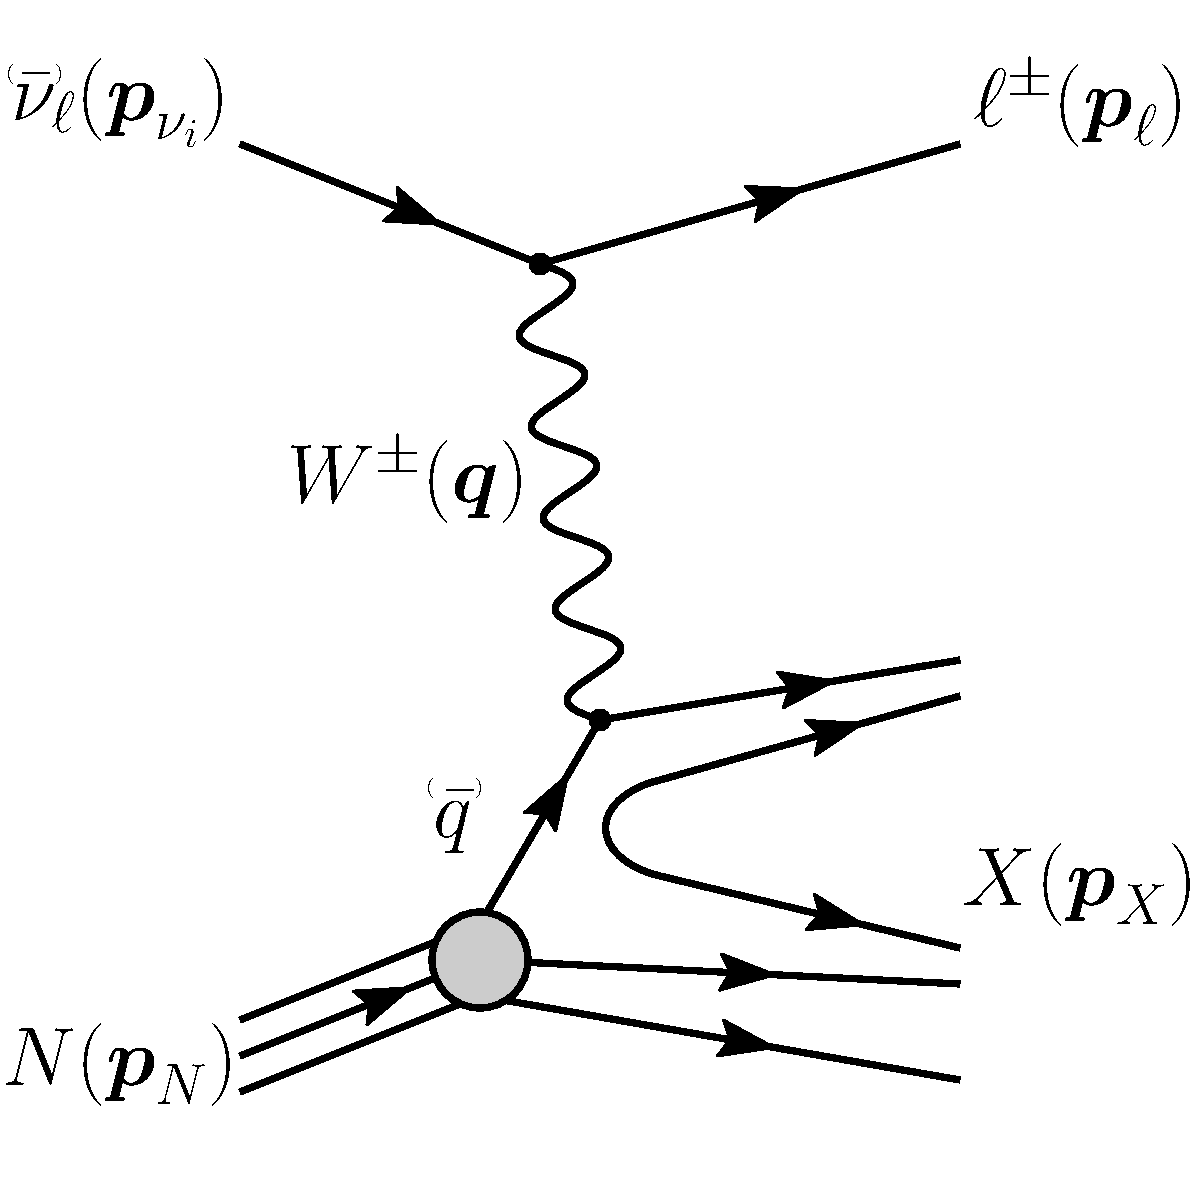
\includegraphics[width=0.4\linewidth]{figures/neutrinos_properties/feynman_DIS_CC_nu_new.pdf}
    \hspace{0.8cm}
    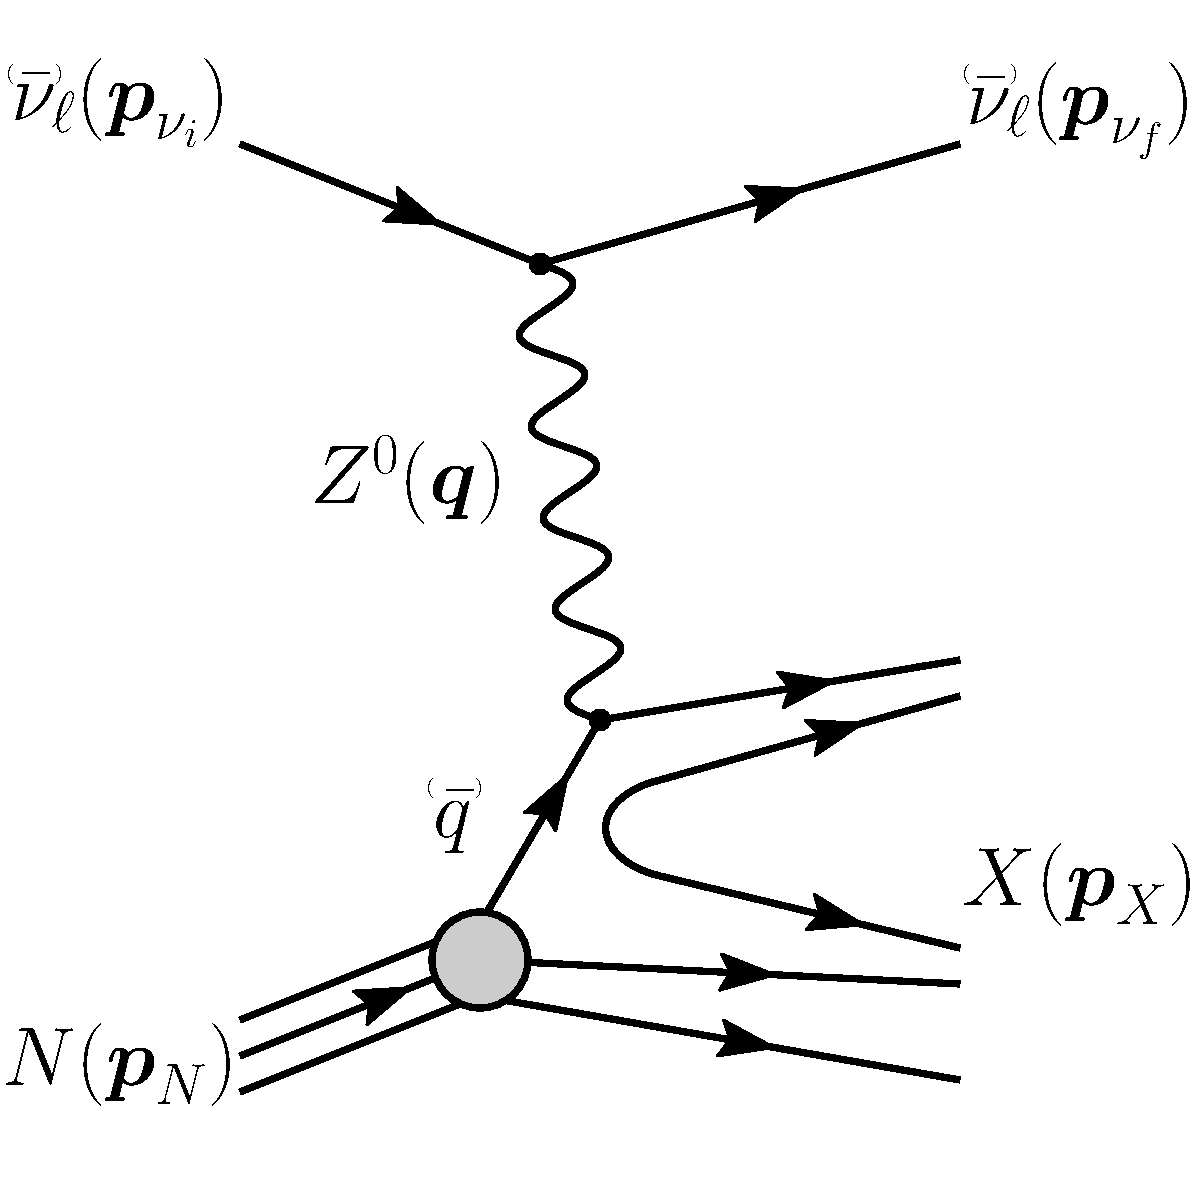
\includegraphics[width=0.4\linewidth]{figures/neutrinos_properties/feynman_DIS_NC_nu_new.pdf}
    \caption[Neutrino-nucleon deep inelastic scattering]{Feynman diagrams for deep inelastic scattering of a neutrino with a nucleon via charged-current (left) and neutral current (right) interactions. $\boldsymbol{p}_{\nu_i}$, $\boldsymbol{p}_{N}$ and $\boldsymbol{p}_{\nu_f}$, $\boldsymbol{p}_{l}$, $\boldsymbol{p}_{N}$ are the input and output four-momenta, while $\boldsymbol{q}$ is the momentum transfer. Taken from \cite{ATerliuk}.}
    \labfig{dis_feynman}
\end{figure}

At energies below \SI{5}{\gev}, \textbf{\textit{quasi-elastic scattering (QE)}} and \textbf{\textit{resonant scattering (RES)}} become important. At these energies the neutrinos interact with the approximately point-like nucleons, without breaking them up in the process. RES describes the process of a neutrino scattering off a nucleon producing an excited state of the nucleon in addition to a charged lepton. It is the dominant process from \SIrange{1.5}{5}{\gev} for neutrinos and from \SIrange{1.5}{8}{\gev} for antineutrinos. Below \SI{1.5}{\gev} QE is the dominant process, where protons are converted to neutrons in antineutrino interactions and vice-versa for neutrino interactions. Additionally, a charged lepton corresponding to the neutrino/antineutrino flavor is produced. The cross-sections of QE and RES scattering processes are not linear in energy and the transition region from QE/RES to DIS is poorly understood. The total cross-sections and their composition is shown in \reffig{neutrino_cross_sections}. It can be seen that the interaction cross-sections are very small at the order of $10^{-38}\mathrm{\,cm}^2$. This is the reason why very large volume detectors are required to measure atmospheric neutrinos with sufficient statistics to perform precision measurements of their properties.

\begin{figure*}[h]
	\centering
    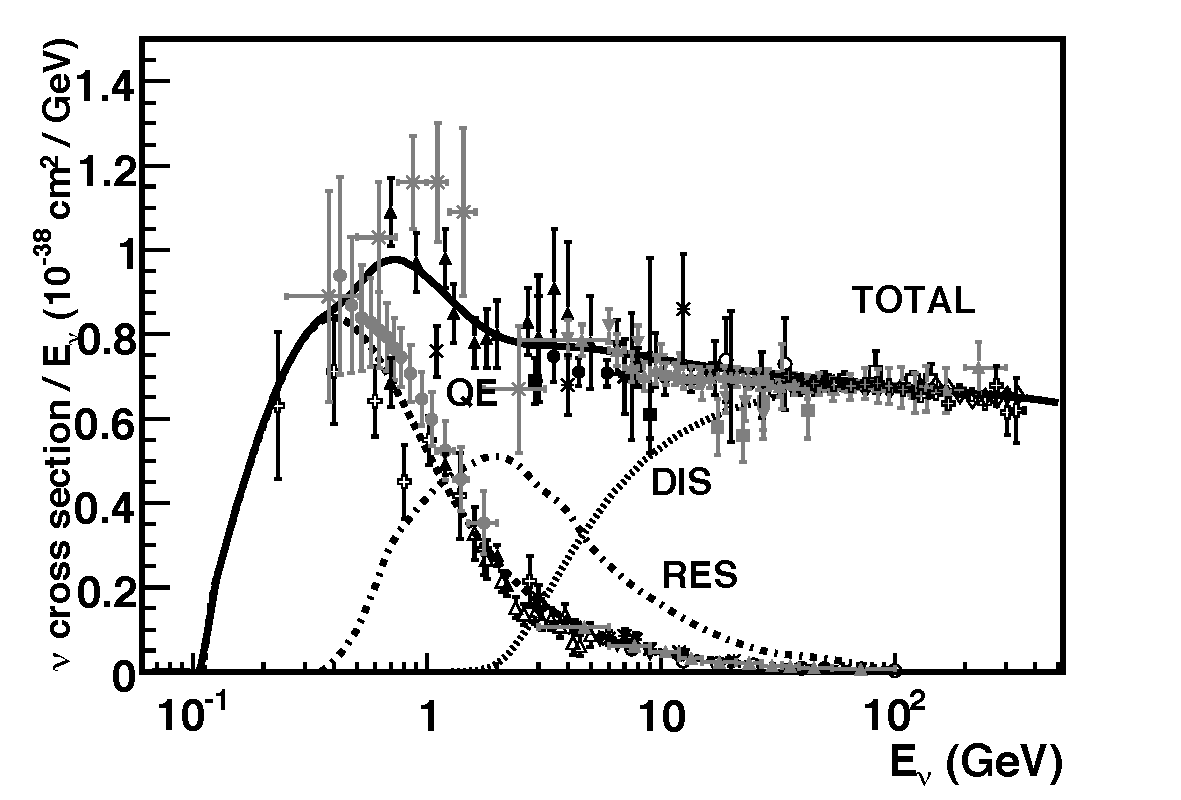
\includegraphics[width=0.495\linewidth]{figures/neutrinos_properties/cc_inclusive_nu.pdf}
    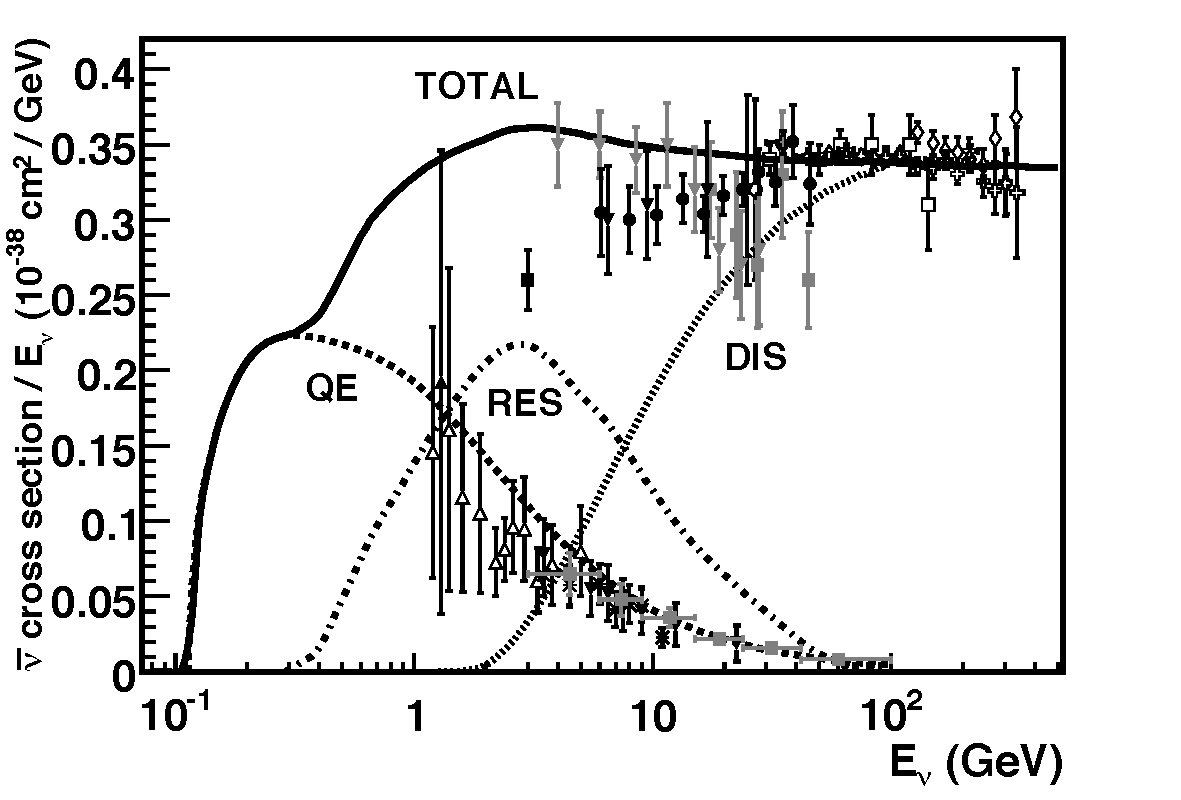
\includegraphics[width=0.495\linewidth]{figures/neutrinos_properties/cc_inclusive_nubar.pdf}
	\caption[Total inclusive neutrino-nucleon cross-sections]{Total neutrino (left) and antineutrino (right) per nucleon cross-section divided by neutrino energy plotted against energy.
    The three main scattering processes quasi-elastic scattering (QE), resonant scattering (RES), and deep-inelastic scattering (DIS) are shown. Taken from \cite{Formaggio_Cross_Sections}.}
    \labfig{neutrino_cross_sections}
\end{figure*}


\subsection{Heavy Neutral Lepton Production and Decay} \labsec{double_cascade_morphology}


For the search conducted in this work, both production and decay of the HNL are assumed to happen inside the detector, therefore probing decay lengths ranges at the scale of the detector size, which is below \SI{1000}{\meter}. Since the mixing with the first two generations of leptons is already strongly constrained as was discussed in \refsec{hnl_theory}, only the mixing with the tau neutrino will be considered in the following. Due to the effect of oscillations, described in \refsec{neutrino_oscillations}, the initial atmospheric muon neutrino flux provides a sizable tau neutrino flux at the detector.

\begin{figure}[h]
    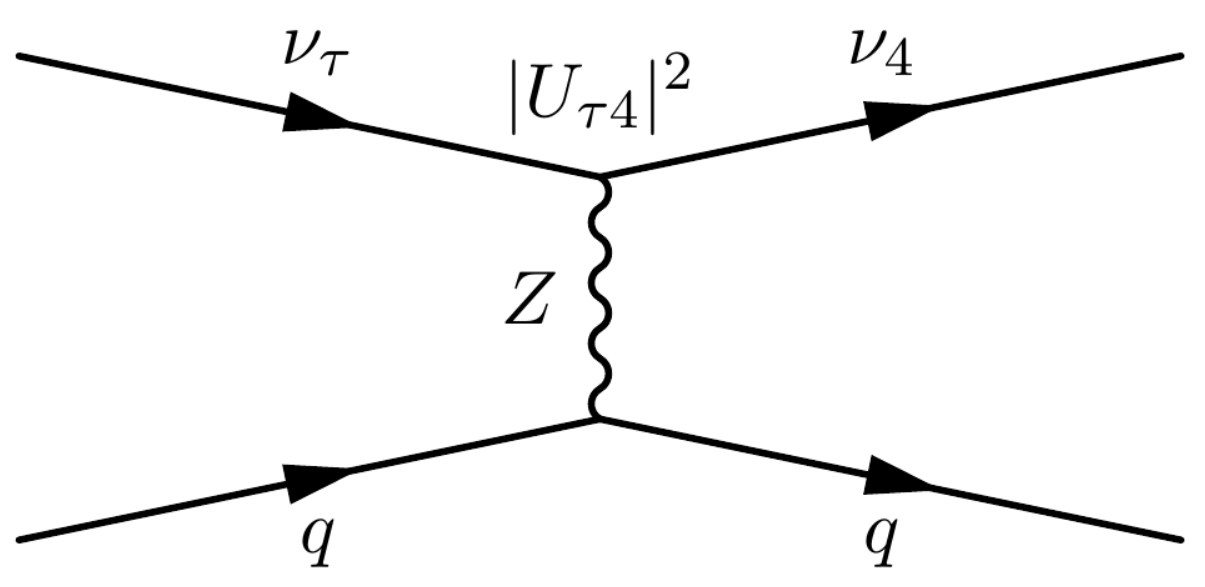
\includegraphics[width=0.5\textwidth]{figures/hnl_simulation/theory/feyn_diags_production.png}
    \caption[Feynman diagram of heavy neutral lepton production]{Feynman diagram of the HNL production. The heavy mass state is produced in the up-scattering of a tau neutrino.}
    \labfig{HNL_production}
\end{figure}

For a non-zero \ut4, the HNL can be produced through \textbf{up-scattering in the ice}. An incoming tau neutrinos scatters on an ice nucleus and transfers some of its kinetic energy to the heavy neutrino. The Feynman diagram of this process is shown in \reffig{HNL_production}. The custom NC cross-sections calculated for this purpose are explained in more detail in \refsec{custom_leptoninjector}, but are similar to the SM tau neutrino NC cross-sections, with a reduction scaling with the mixing \ut4 and energy dependent reductions, due to kinematic constraints because of the heavy neutrino mass. The scattering process produces a hadronic cascade, which will produce light in the detector.

\begin{figure}[h]
    \includegraphics{figures/hnl_simulation/theory/feyn_diags_decay.png}
    \caption[Feynman diagram of heavy neutral lepton decay]{Feynman diagram of the HNL decay. The heavy mass state can decay through neutral current interaction (left) into a tau neutrino and a charged lepton or quark pair, or through charged current interaction (right) into a tau lepton and a charged lepton or quark.}
    \labfig{HNL_decay}
\end{figure}

After a certain distance, the HNL will \textbf{decay in the ice}, where the possible decay channels considered in this work and the underlying, explicit calculations are discussed in \refsec{custom_leptoninjector}. The decay can be a CC or NC and both purely leptonic and leptonic+mesonic modes are possible. The Feynman diagrams of the decays can be seen in \refsec{HNL_decay}. Only the mass range relevant for this work is presented and mixing with $\nu_{e/\mu}$ is assumed to be negligible. Depending on the decay channel, an electromagnetic or a hadronic cascade is produced, while some energy is carried away by the invisible neutrino. The decay length of the HNL is defined by its proper lifetime\sidenote{A particle decay time follows an exponential distribution, with mean lifetime given by the proper lifetime. The proper lifetime is the lifetime in the rest frame of the particle.}, which is given by
\begin{equation}
    \tau_\mathrm{proper} = \frac{\hbar}{\Gamma_\mathrm{total}(m_4) \cdot |U_{\tau4}|^2}
    \;,
    \labeq{proper_lifetime_v0}
\end{equation}
where $\hbar$ is the reduced Planck constant, $\Gamma_\mathrm{total}(m_4)$ is the total decay width of the HNL for the given mass, and $|U_{\tau4}|^2$ is the mixing with the tau neutrino. The total decay width is the sum of the partial decay widths for all possible decay channels. The mean lab frame decay length is then given by
\begin{equation}
    L_\mathrm{decay} = \gamma v \tau_\mathrm{proper}
    \;,
    \labeq{decay_length}
\end{equation}
where $\gamma$ is the Lorentz factor of the HNL, defined by the kinetic energy. This will be further discussed on \refsec{custom_leptoninjector}. \reffig{hnl_decay_lengths} shows the mean decay lengths for an example mass of $m_4=\SI{0.6}{\gev}$ and several mixing values.

\begin{figure}[h]
    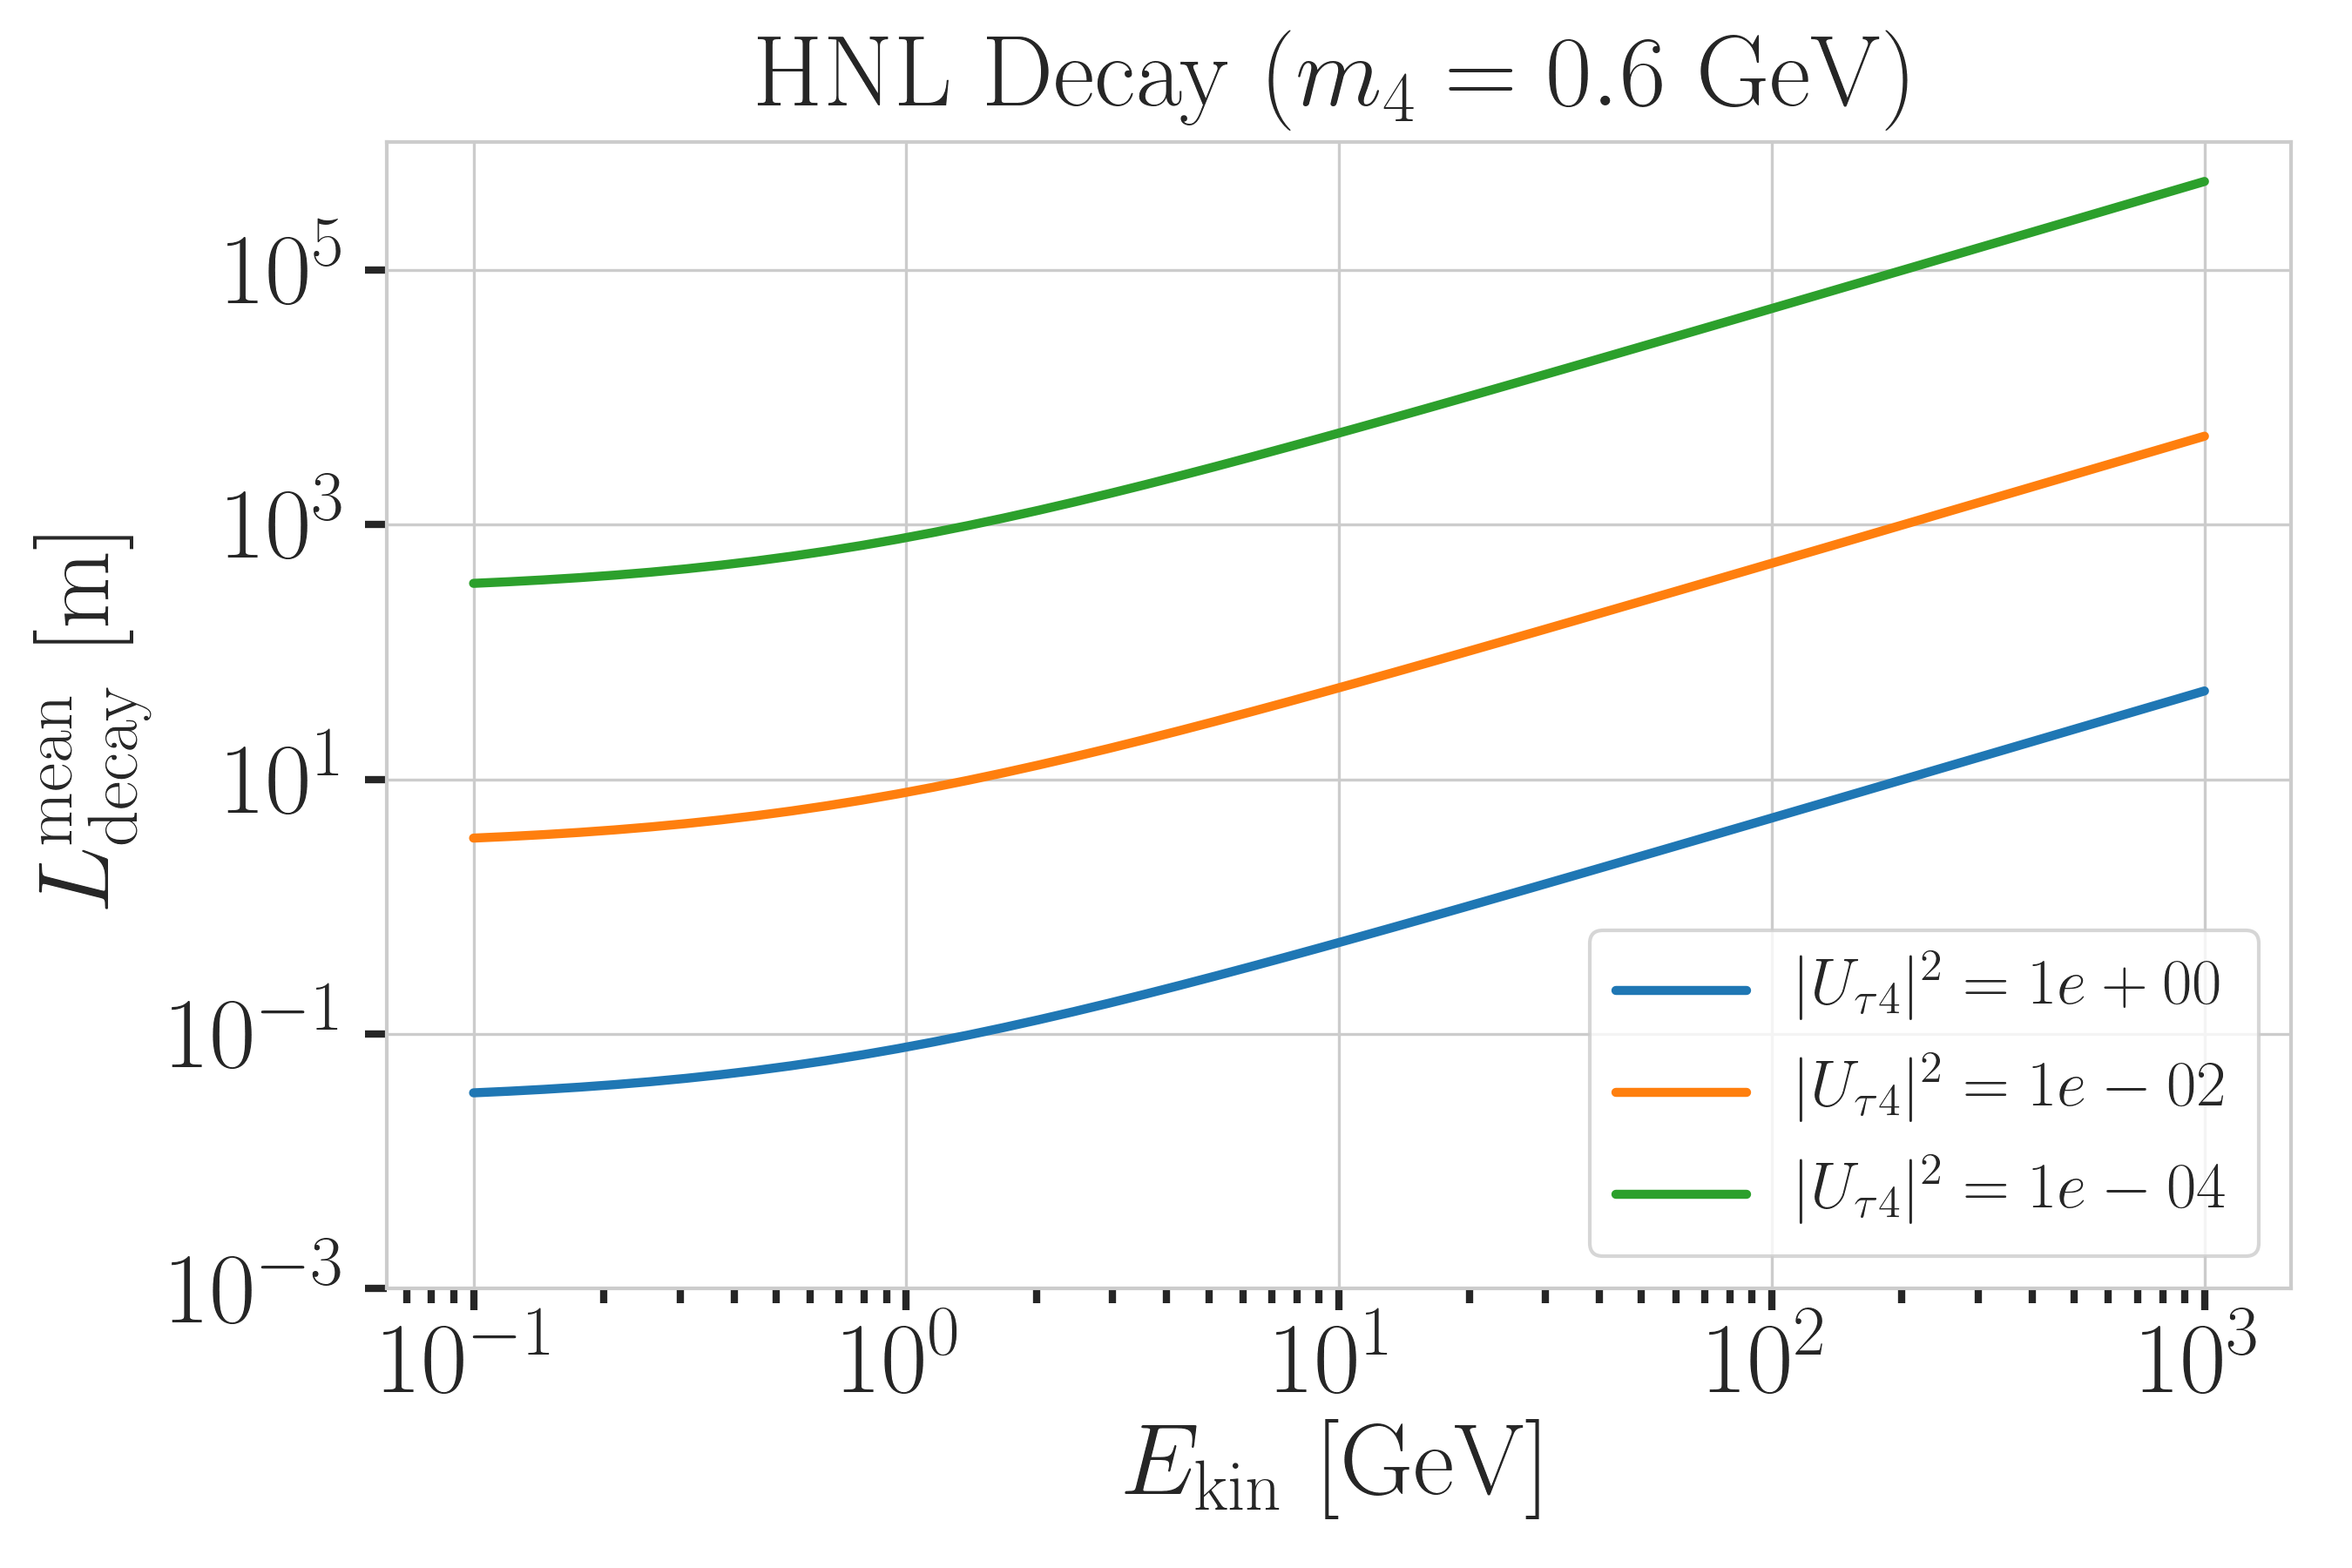
\includegraphics{figures/hnl_simulation/theory/decay_length_vs_energy_m4_6e-01.png}
    \caption[Theoretical mean HNL decay length (\SI{0.6}{\gev} mass)]{Theoretical mean decay length of the HNL for a mass of \SI{0.6}{\gev} and different mixing values.}
    \labfig{hnl_decay_lengths}
\end{figure}


\setchapterstyle{kao}
\setchapterpreamble[u]{\margintoc}


\chapter{The IceCube Neutrino Observatory}
\labch{icecube}

The IceCube Neutrino Observatory \sidecite[6cm]{2017JInst..12P3012A_Instrumentation_Systems} is a cubic-kilometer, ice-Cherenkov detector located at the geographic South Pole. IceCube utilizes the Antarctic glacial ice as detector medium to observe neutrinos by measuring the Cherenkov light produced from secondary charged particles. It was deployed between 2006 and 2011 and has been taking data since the installation of the first modules. The primary goal of IceCube is the observation of astrophysical neutrinos as a telescope, but it can also be used to study fundamental particle physics properties by measuring atmospheric neutrinos as well as studying cosmic rays.

This chapter first describes the main- and sub-array of the detector and its detection module in \refsec{icecube_array}, the propagation of particles through ice is explained in \refsec{icecube_propagation}, and finally, the signatures that IceCube can observe of the different particles are introduced in \refsec{icecube_signatures}.


\section{Detector Components} \labsec{icecube_array}

\begin{figure}[h]
    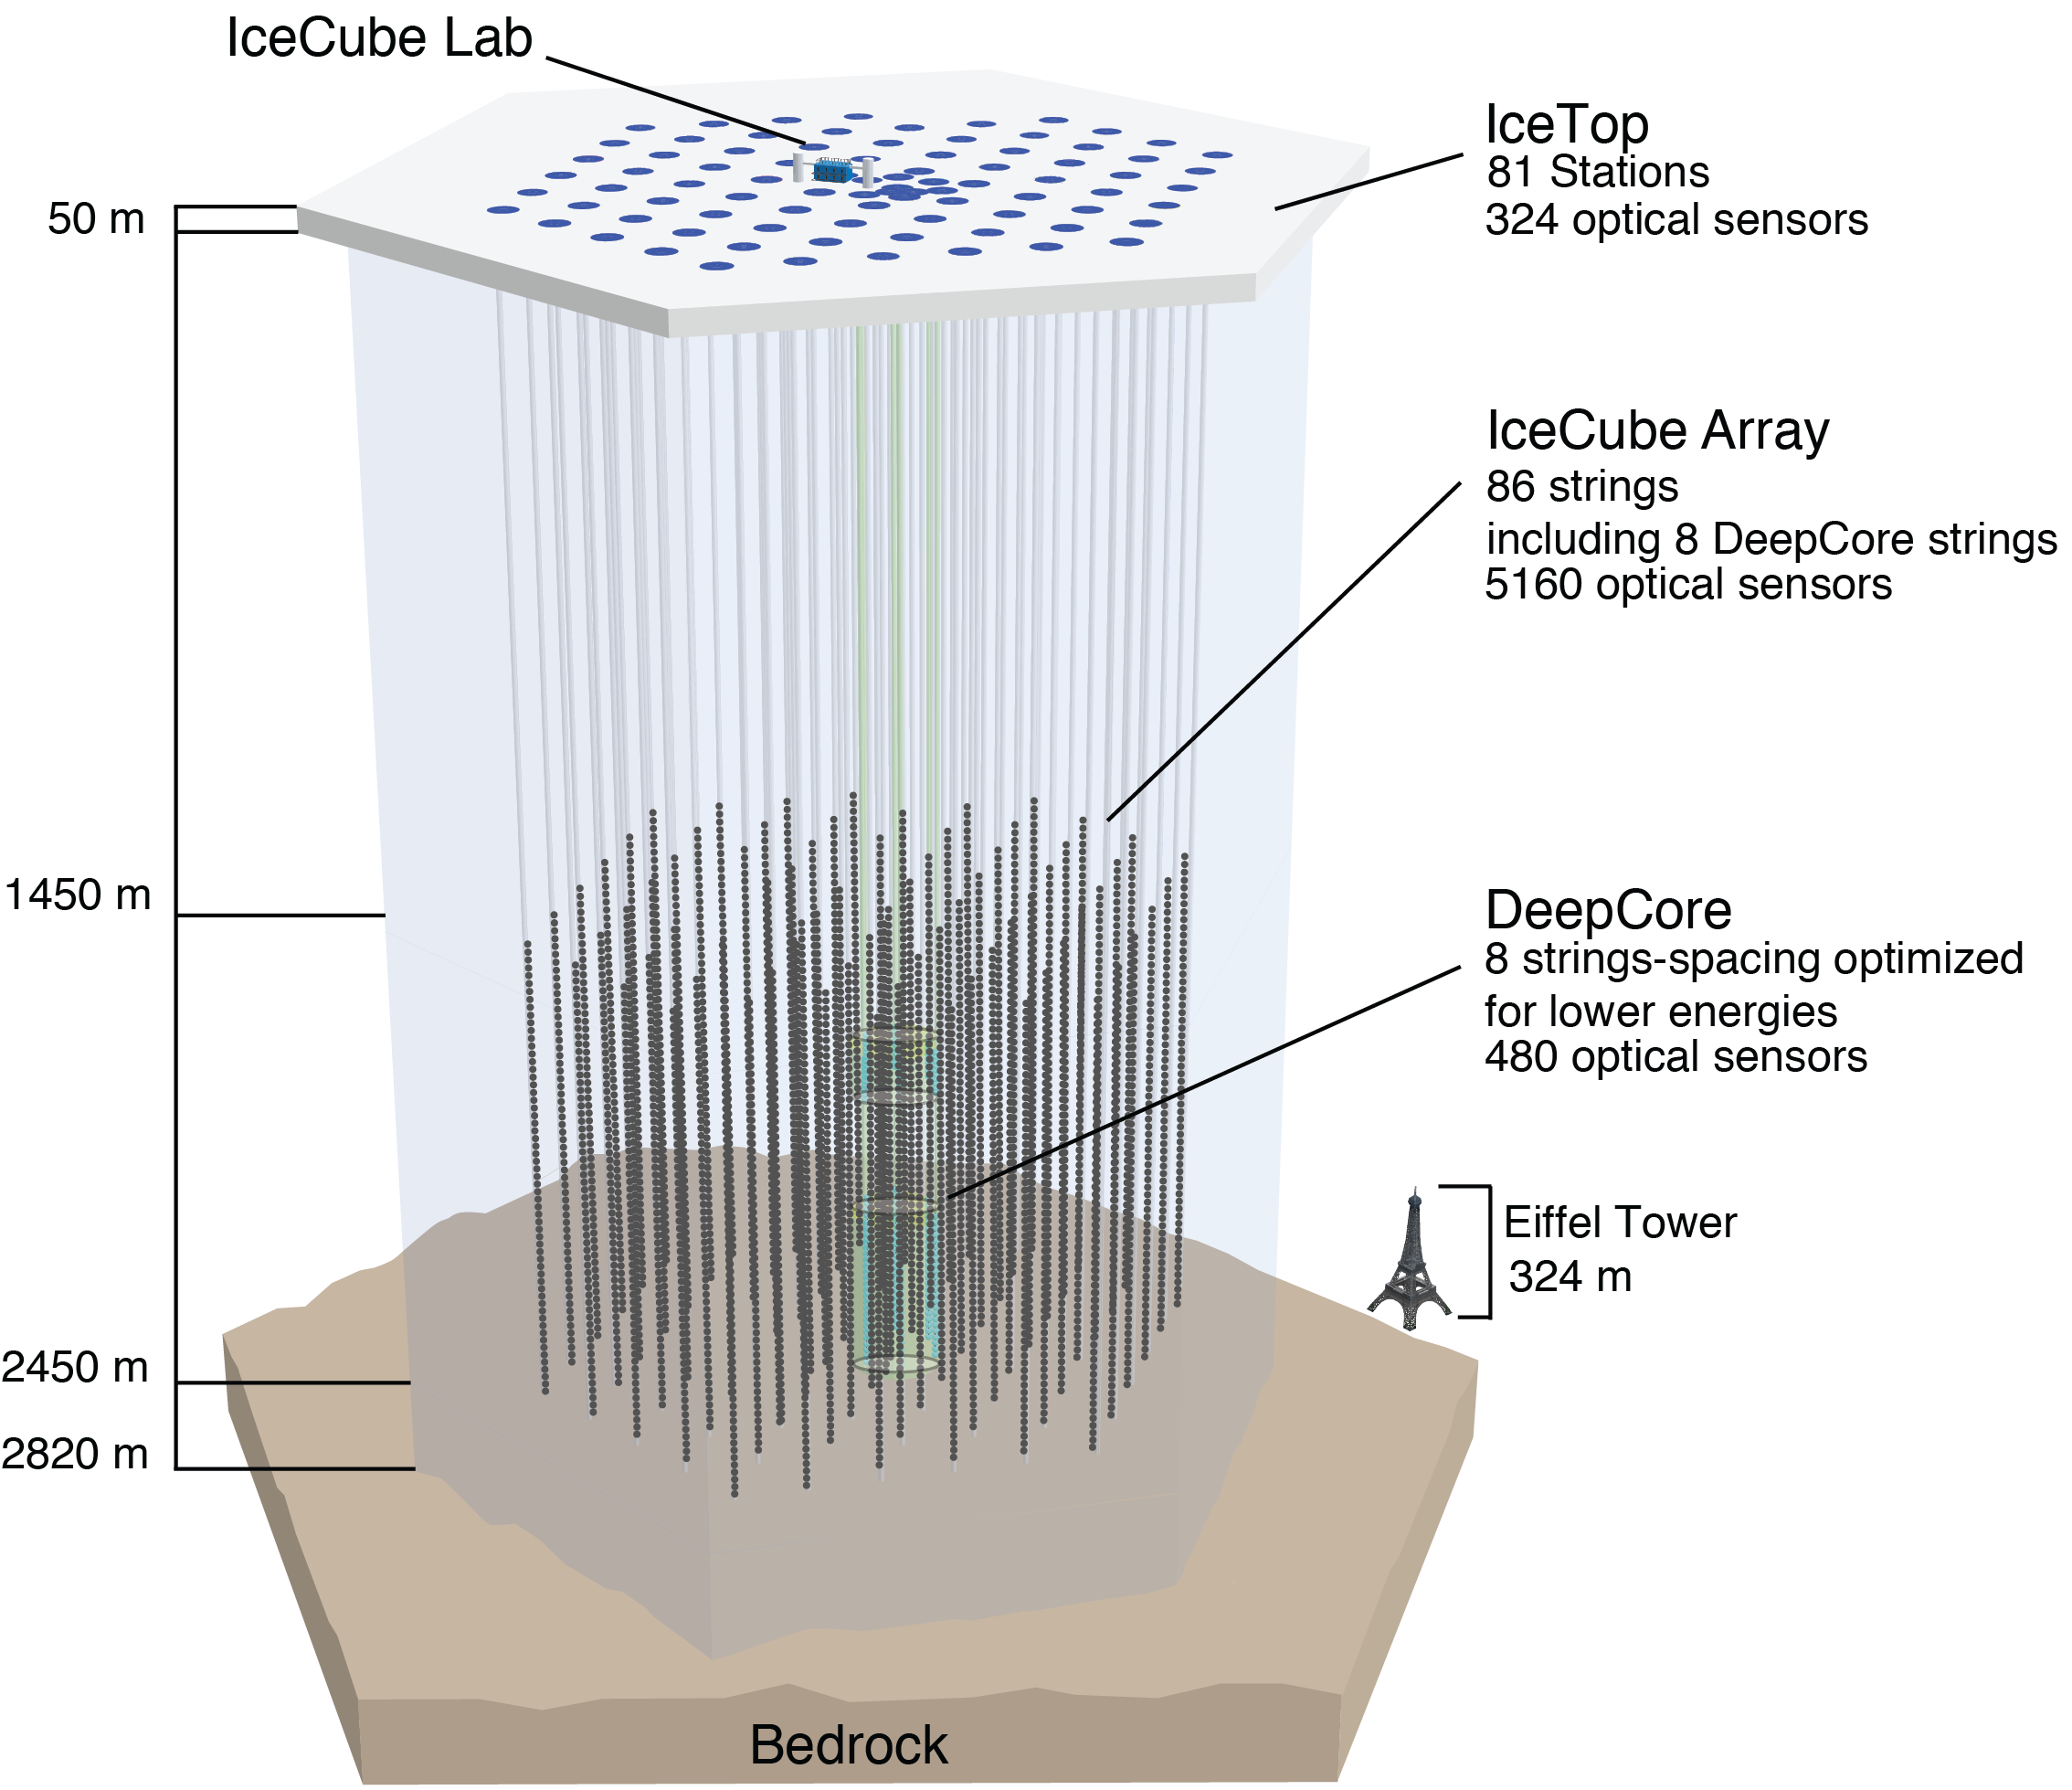
\includegraphics{figures/icecube_deepcore/IceCubeArray_slim.png}
	\caption[IceCube overview]{Overview of the IceCube detector showing the in-ice main- and sub-array IceCube and DeepCore, IceTop, and the IceCube Laboratory. From \cite{2017JInst..12P3012A_Instrumentation_Systems}.}
    \labfig{icecube_array}
\end{figure}

The full IceCube detector array consists of 86 vertical, in-ice strings and 81 surface stations as shown in \reffig{icecube_array}. The in-ice part is composed of 60 optical modules per string deployed at depths of \SIrange[range-phrase={~-~}]{1450}{2450}{\meter} below the ice, while the surface stations of the cosmic air-shower array, \textit{IceTop}, are ice-filled tanks. The surface stations and the majority of the strings are arranged in a hexagonal grid with the operations building, the \textit{IceCube Laboratory} (ICL), central to the grid on the surface. A top view of the hexagonal arrangement is shown in \reffig{icecube_top_view}. The in-ice array is designed to detect neutrinos in the energy range from \si{\giga\electronvolt} to \si{\peta\electronvolt}.


\subsection{Digital Optical Modules and the Antarctic Ice} \labsec{ice_and_DOMs}

The IceCube detection medium is the Antarctic glacial ice itself, which was formed over \SI{100000}{years} by accumulation of snow that was subsequently compressed by its own weight to form a dense crystal structure \sidecite{glacial_ice}. As a result of this formation process, the optical properties, scattering and absorption\todo{SB:
there are more properties than just these. Somehow need a half sentence that explains why these are particularly important to single out (see ice papers for inspiration) (ORANGE)
}, primarily change with depth. Within the detector volume the absorption length ranges from \SIrange[range-phrase={~-~}]{100}{400}{\meter}, while the scattering length lies between \SIrange[range-phrase={~and~}]{20}{100}{\meter}\todo{CL:
maybe define that absorption and scattering lengths are? they are defined differently so this invites a comparison that is not so obvious (ORANGE)
}. They are correlated, with the absorption length being roughly four times the scattering length \sidecite{ice_calibration}. The vertical distribution of scattering and absorption length can be seen in \reffig{ic_dc_sidecut}, where one dominant feature is the \textit{dust layer} between \SIrange[range-phrase={~and~}]{2000}{2100}{\meter} depth. This region has a higher concentration of dust particles that were deposited in a period of high volcanic activity, which leads to bad optical properties in form of larger scattering and absorption.\todo{Add reference for the dust layer! Maybe also from the ice paper? mention/cite dust logger paper/procedure? (ORANGE)}


\begin{figure}[h]
    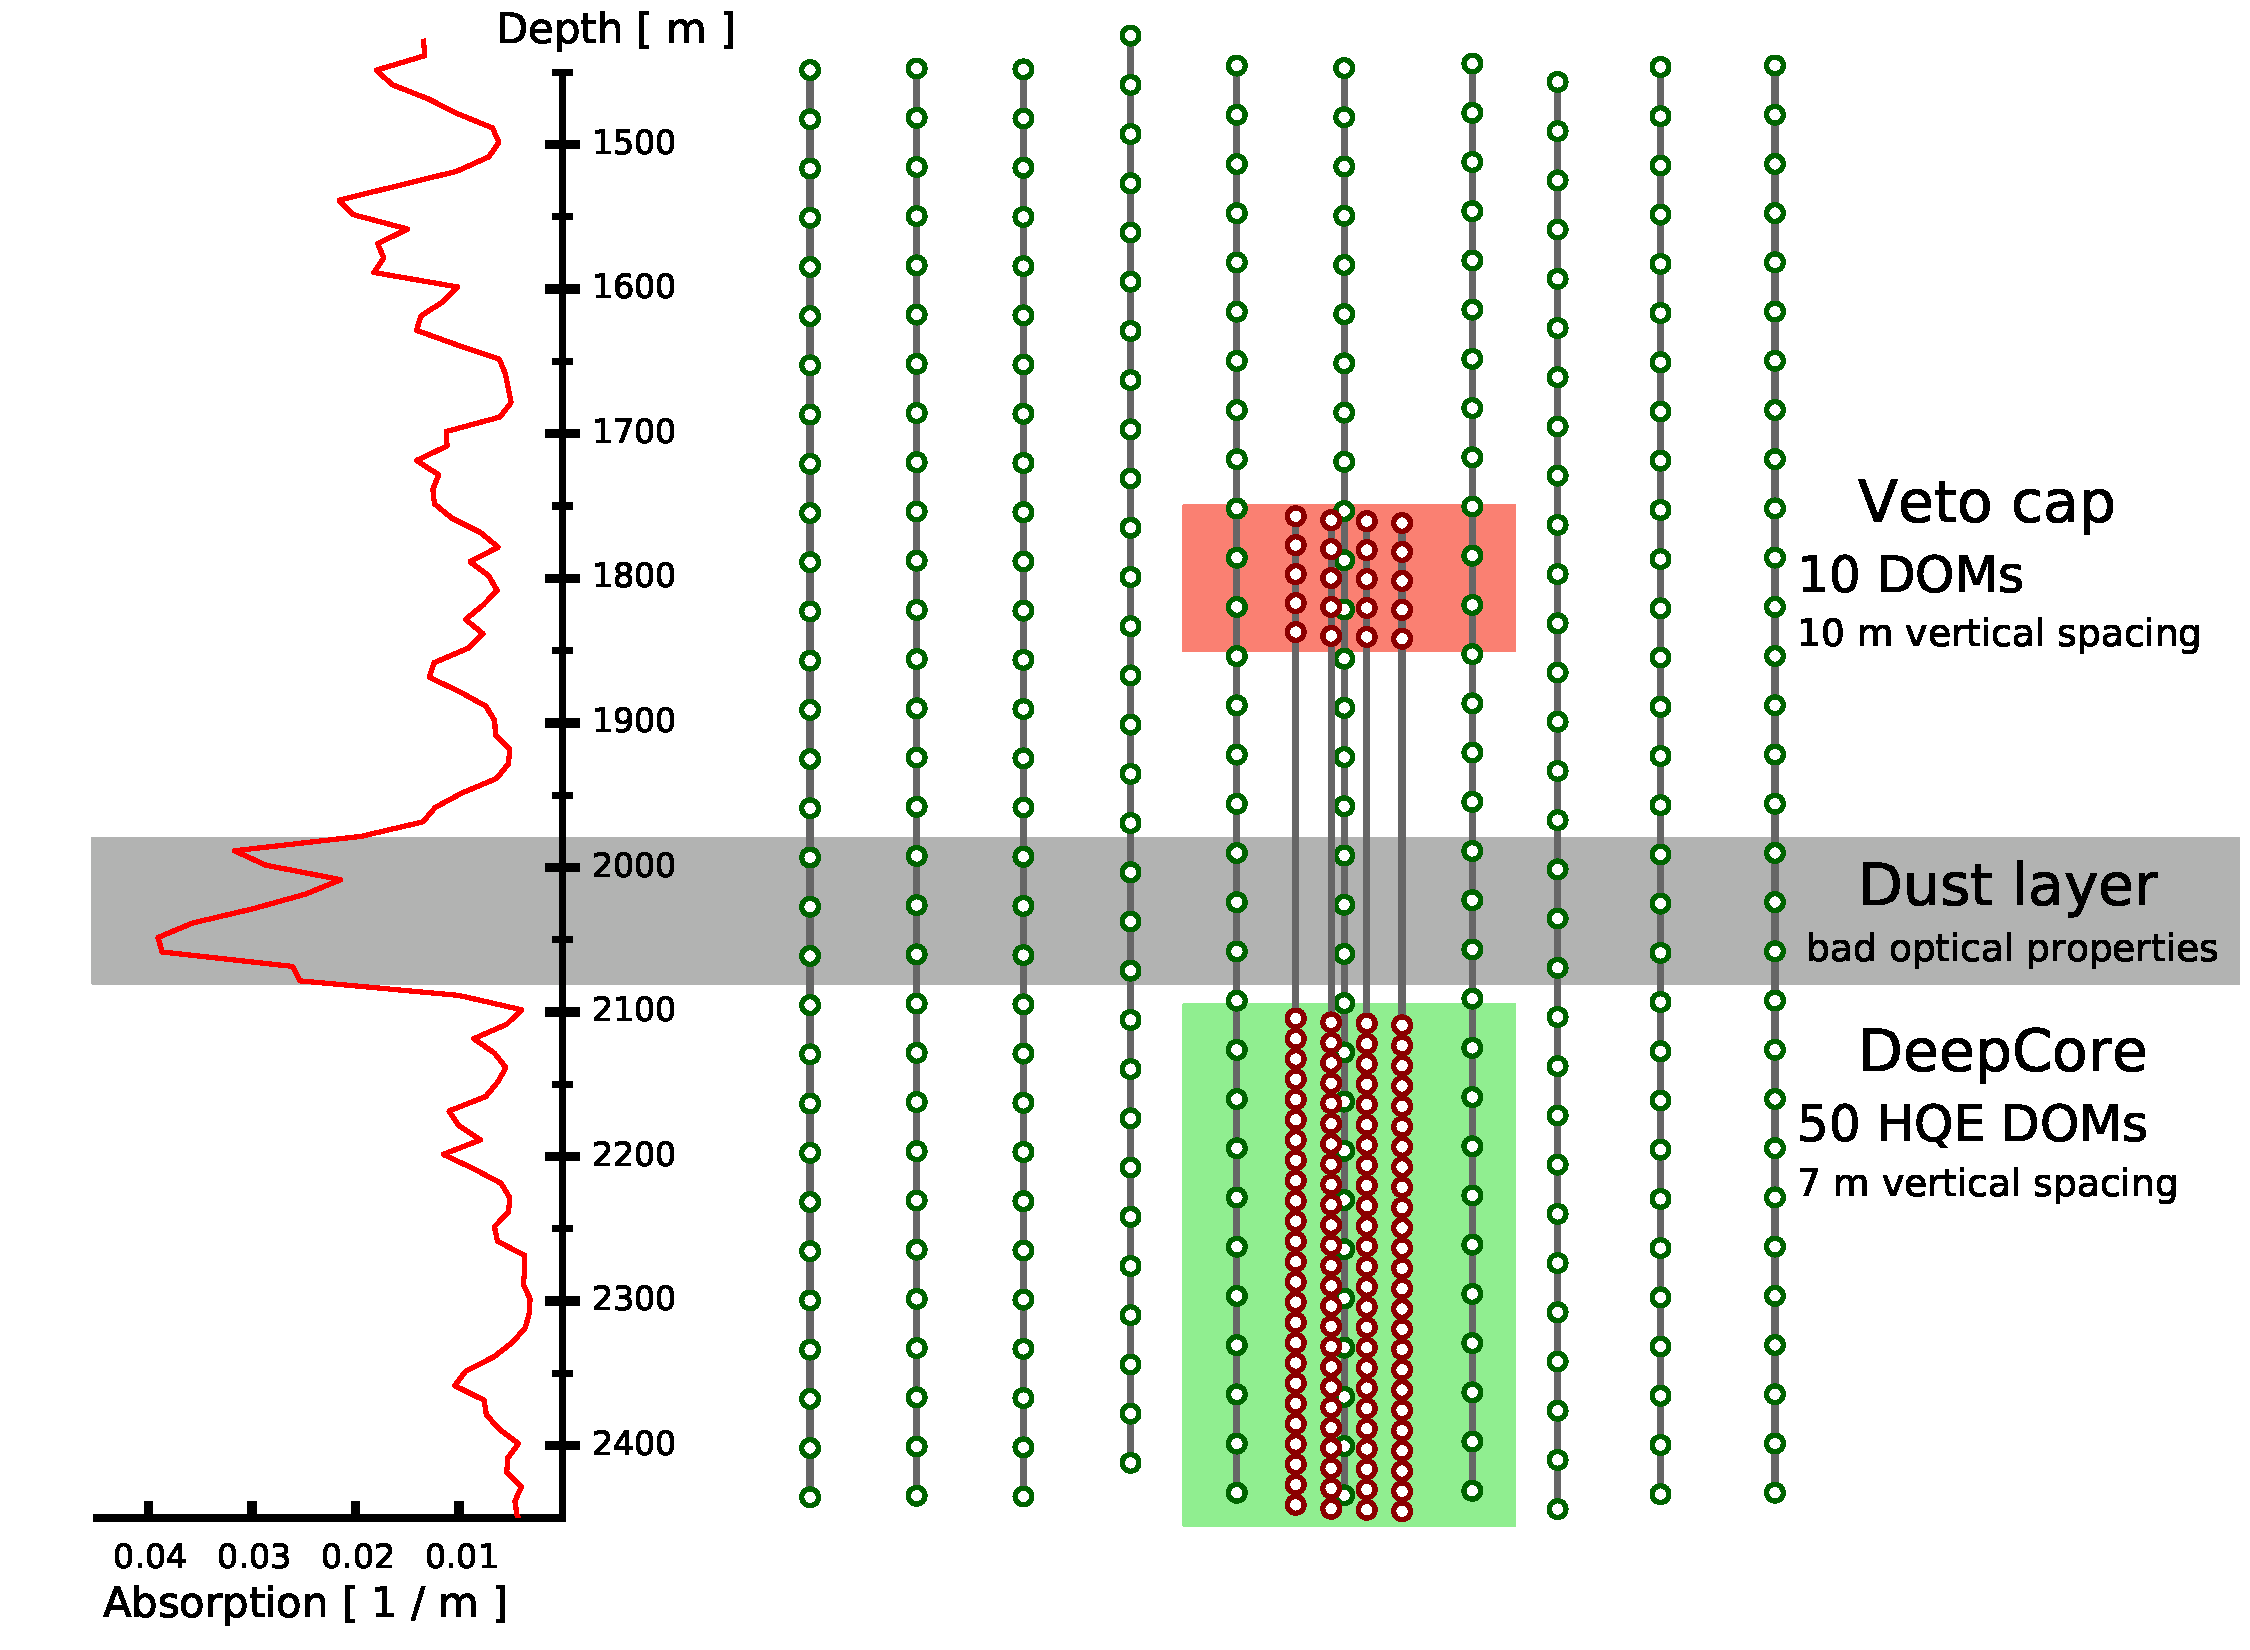
\includegraphics{figures/icecube_deepcore/DeepCore_sideview.pdf}
	\caption[IceCube side view]{Side view of IceCube and DeepCore showing the depth dependent scattering and absorption length (left panel) and the DOM positions around the dust layer.}
    \labfig{ic_dc_sidecut}
\end{figure}

\todo{exchange for figure with scattering (check abs/sca is correct) (ORANGE)}

The ice is instrumented by 5160 optical sensors called \textit{digital optical modules} (DOMs) \sidecite{ABBASI2009294_data_acquisition}, which can detect the Cherenkov light produced by charged particles traveling through the ice. Each DOM is made of a spherical glass housing, containing a downward-facing Photomultiplier Tube (PMT), the main-board with control, readout, and processing-electronics, and a LED flasher-board for calibration purposes. The design and the individual components of a DOM can be seen in \reffig{DOM_design}.

The majority of PMTs are the \SI{10}{"} Hamamatsu R7081-02, which have a bialkali photocathode and are sensitive to wavelengths in the range of \SIrange{300}{650}{\nano\meter}, with a peak quantum efficiency of 25\% at \SI{390}{\nano\meter}. In the central part of the IceCube array the peak efficiency reaches 34\%. The dark count rate in the temperature range of \SIrange{-40}{-20}{\degreeCelsius} is $\sim$\SI{300}{\hertz}. The DOM electronics measure the PMT voltage and control the gain. At a voltage crossing of the equivalent to \SI{0.25}{PE} the waveform readout is activated \sidecite{ABBASI2009294_data_acquisition}. Only when either one of the nearest or next to nearest DOMs above or below also sees a voltage crossing within a \SI{1}{\micro\second} time window \sidenote{This is referred to as a \textit{hard local coincidence (HLC)} \cite{ABBASI2009294_data_acquisition}.}, the voltages are digitized and sent to the ICL. Through the application of a waveform unfolding algorithm, called \textit{WaveDeform} \sidecite{IceCube:2013dkx}, the waveforms are compressed, and the results are the reconstructed times and charges of the photo-electrons. This is the basis for all further IceCube data processing.

\begin{marginfigure}
    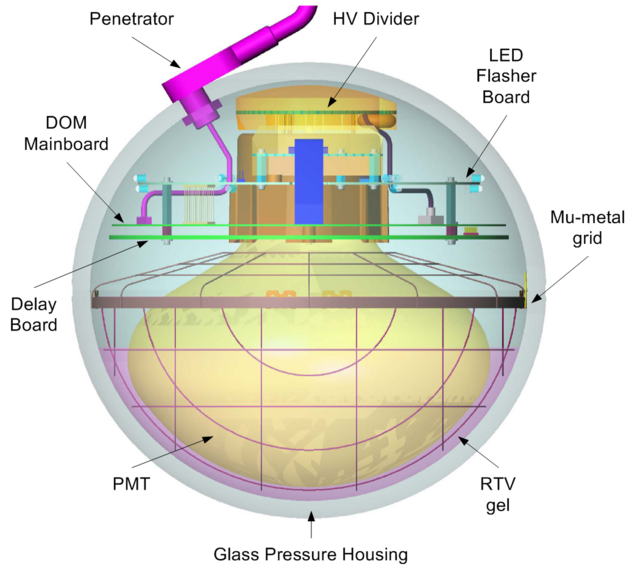
\includegraphics{figures/icecube_deepcore/DOM_schematic.png}
	\caption[Digital optical module (DOM)]{Design and components of a digital optical module (DOM) \cite{ABBASI2009294_data_acquisition}}
    \labfig{DOM_design}
\end{marginfigure}

The PMT is covered with a mu-metal grid (made from wire mesh), shielding the photocathode from Earth's magnetic field, and it is optically coupled to the glass sphere by RTV silicone gel. The glass sphere is a pressure vessel, designed to withstand both the constant ice pressure and the temporary pressure during the refreezing process of the water in the drill hole during deployment (peaking at around \SI{690}{\bar}). The sphere is held by a harness that connects the DOMs along a string and also guides the cable beside them.

The flasher-board controls 12 LEDs that produce optical pulses with a wavelength of \SI{405}{\nano\meter} \sidecite{2017JInst..12P3012A_Instrumentation_Systems}. The LEDs can be pulsed separately or in combination with variable output levels and pulse lengths. Using the known information of the light source positions and times this can be used for in-situ calibration of the detector by measuring absorption and scattering properties of the ice. Calibrating the absolute efficiency of the DOMs itself is more accurately done using minimum ionizing muons \sidecite{JFeintzeig_phd, domeff_nick}, since the total amplitude of the LED light is not well known.\todo{Add accuracy of the efficiency calibration here. (ORANGE)}


\subsection{IceCube Main-Array} \labsec{icecube}

\begin{figure}
    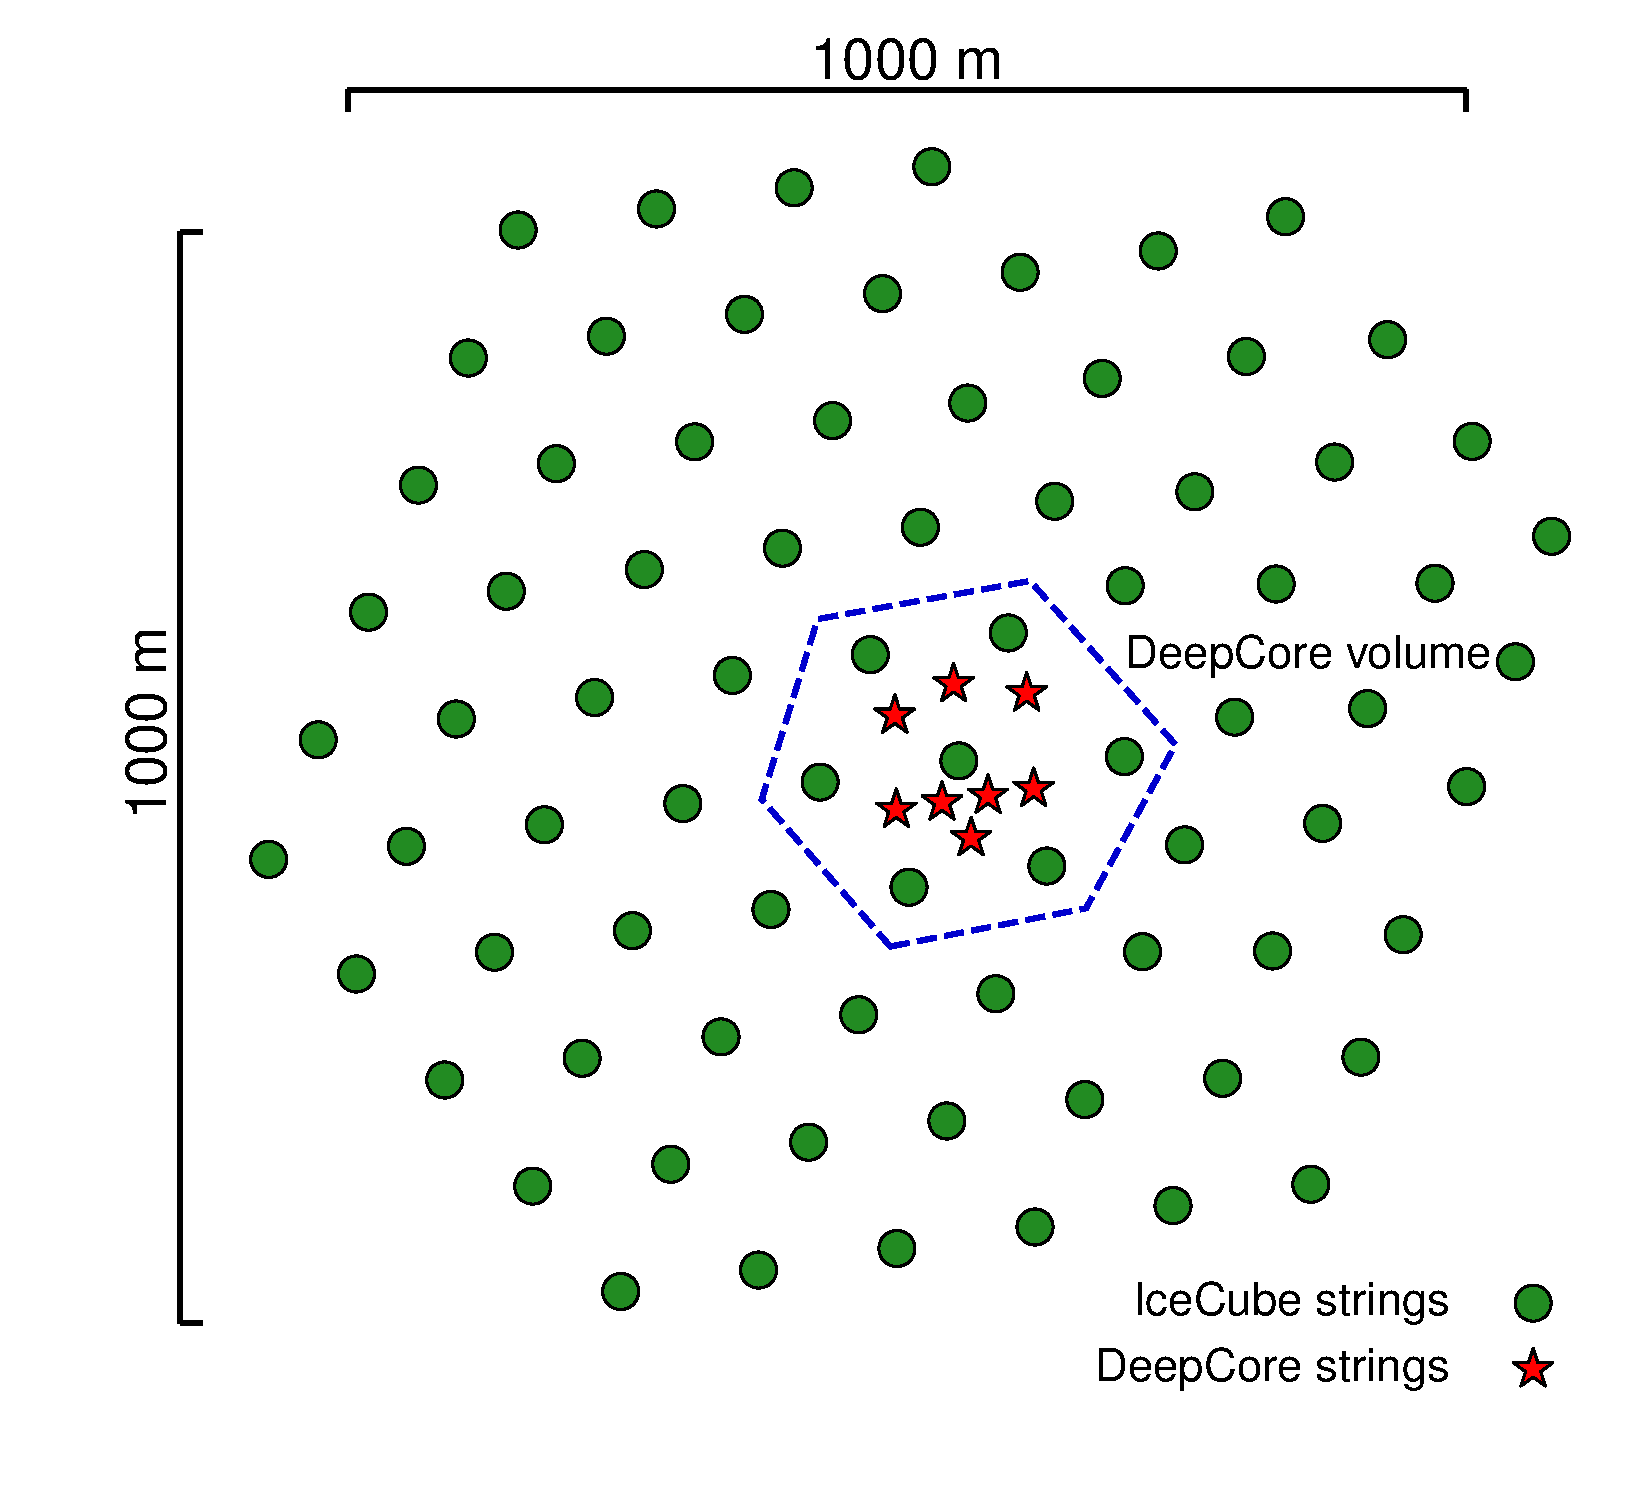
\includegraphics[trim={2.0cm, 1.5cm, 0, 0}, clip, width=0.65\linewidth]{figures/icecube_deepcore/icecube_top_view_bw.pdf}
    % 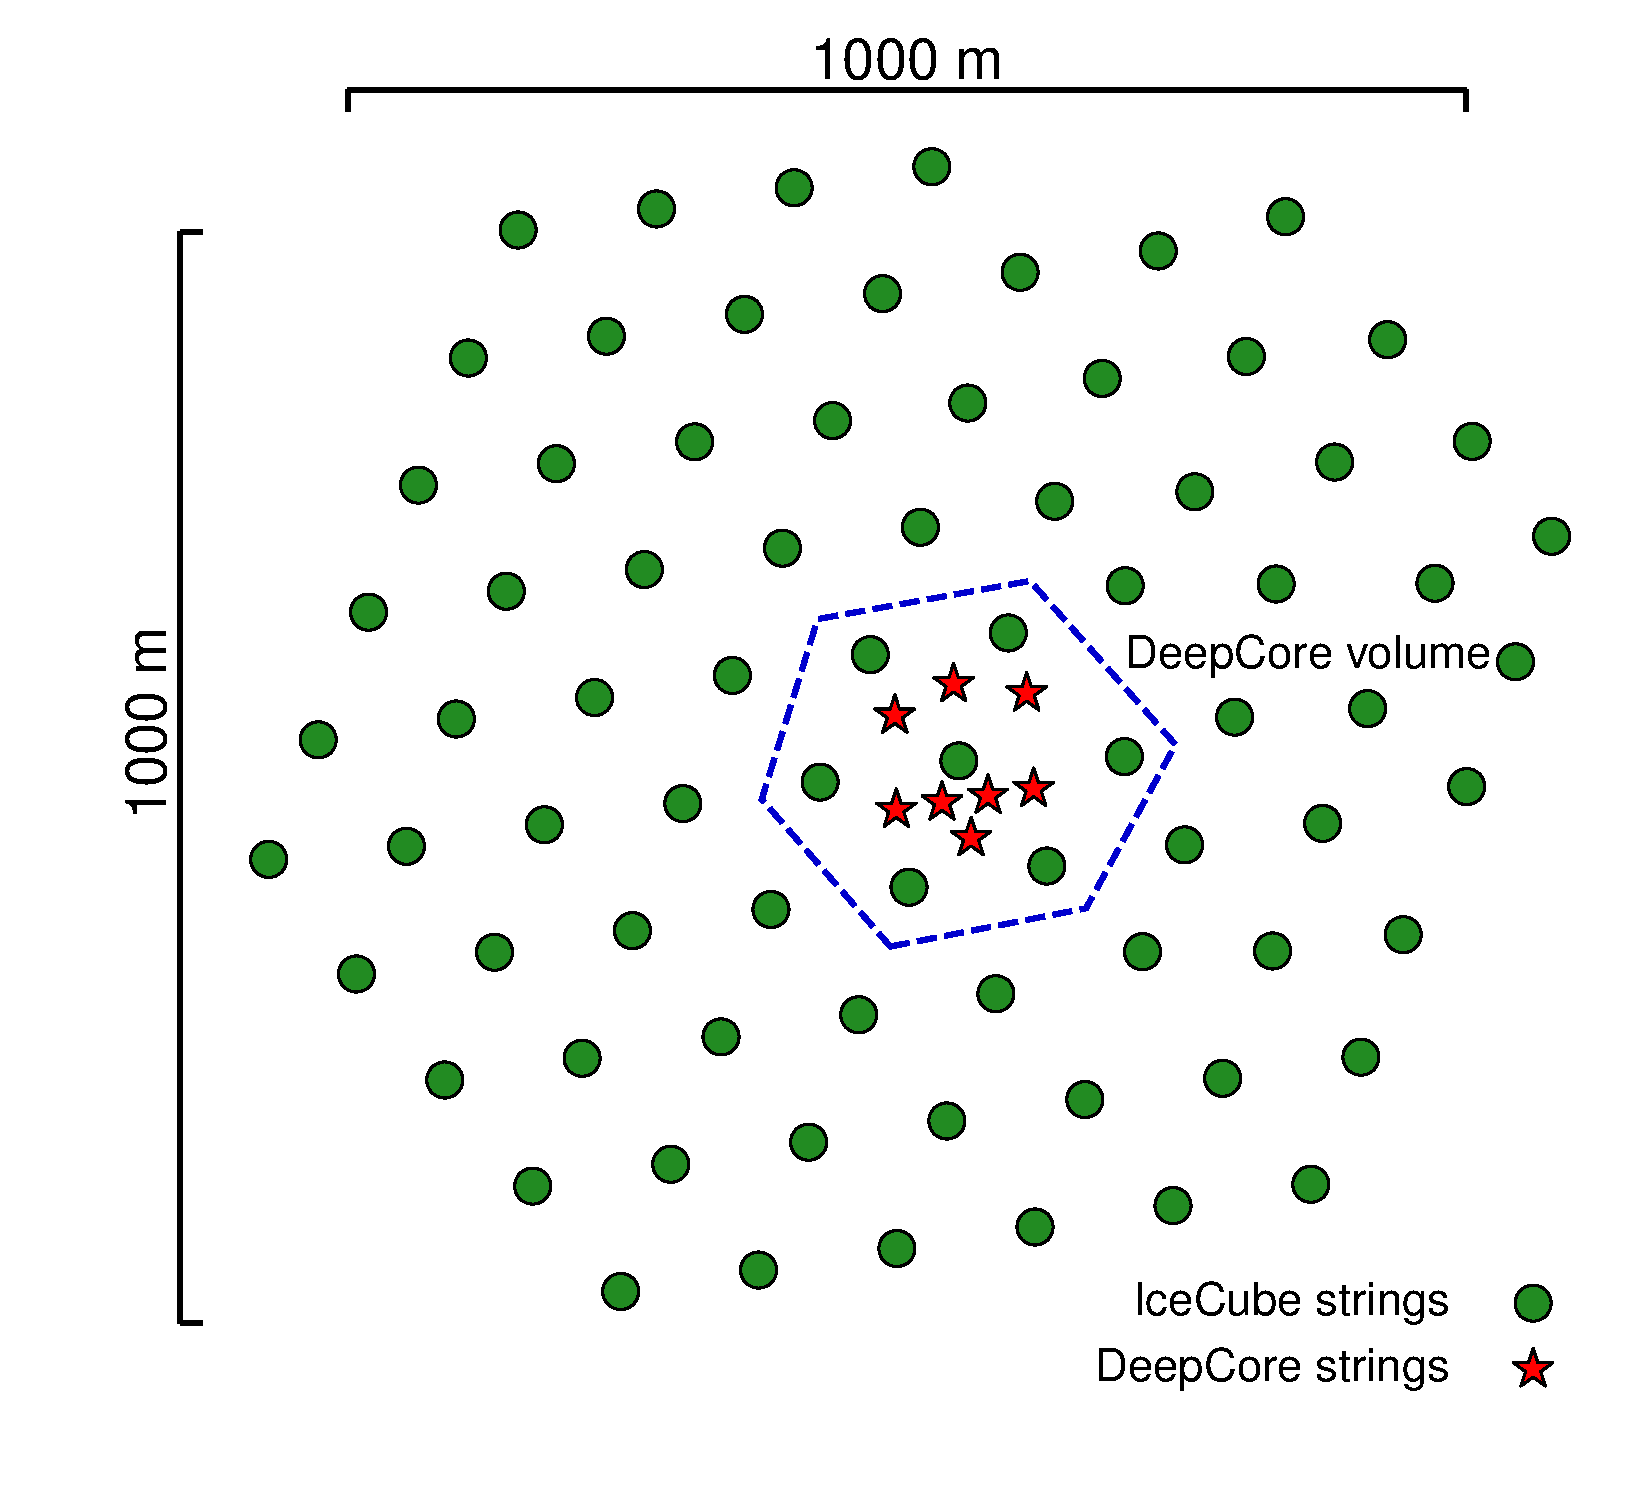
\includegraphics[trim={2.0cm, 1.5cm, 0, 0}, clip, width=1.0\linewidth]{figures/icecube_deepcore/icecube_top_view_bw.pdf}
    \caption[IceCube top view]{Top view of the IceCube array.}
    \labfig{icecube_top_view}
\end{figure}

The 78 strings that are arranged in a hexagonal pattern from the main part of the in-ice array, which is called \textit{IceCube}. With a $\sim$\SI{125}{\meter} horizontal spacing between the strings and a $\sim$\SI{17}{\meter} vertical spacing between DOMs, IceCube has a lower energy threshold of around \SI{100}{\gev}. IceCube was designed to detect astrophysical neutrinos with energies above \SI{1}{\tera\electronvolt}.

The coordinate system that is used in IceCube is centered at 46500'E, 52200'N at an elevation of \SI{883.9}{\meter} \sidecite{2017JInst..12P3012A_Instrumentation_Systems}. Per definition, it's a right-handed coordinate system where the y-axis points along the Prime Meridian (Grid North) towards Greenwich, UK, and the x-axis points \SI{90}{\degree} clockwise from the y-axis (Grid East). The z-axis is normal to the ice surface, pointing upwards. For IceCube analyses depth is defined as the distance along the z axis from the ice surface, assumed to be at an elevation of \SI{2832}{\meter}.


\subsection{DeepCore Sub-Array} \labsec{deepcore}

The additional 8 strings form a denser sub-array of IceCube called \textit{DeepCore} \sidecite{DeepCore_design_Abbasi2012615}. It is located at the bottom-center of the in-ice array and its \textit{fiducial volume} also includes the 7 surrounding IceCube strings as shown in \reffig{icecube_top_view}. The strings in this region have a closer average horizontal distance of about \SI{70}{\meter}. The lower 50 DeepCore DOMs on each string are placed in the region of clear ice below the dust layer between \SIrange{2100}{2450}{\meter} depth, where their vertical spacing is $\sim$\SI{7}{\meter}. The remaining 10 modules on each string are placed above the dust layer to be used as veto against atmospheric muons as can be seen in \reffig{ic_dc_sidecut}. Additionally, the DeepCore DOMs are equipped with higher quantum efficiency PMTs\sidenote{At \SI{400}{\nano\meter} they are \SI{35}{\percent} more efficient than the IceCube PMTs \cite{DeepCore_design_Abbasi2012615}.}. The combination of the denser spacing, the high quantum efficiency modules, and the most favorable ice properties below the dust layer leads to a lower energy detection threshold of around \SI{5}{GeV}, allowing the more efficient observation of atmospheric neutrinos.
, which are mostly in the energy range of \SIrange[range-phrase={~-~}]{10}{100}{\giga\electronvolt}.
Atmospheric neutrino oscillation analyses result in competitive measurements of the neutrino mixing parameters \sidecite{OVS_PRD, flercnn_analysis_result}, but the large flux of atmospheric neutrinos allows for many BSM searches, such as searches for dark matter, non-standard interactions, or sterile neutrinos.


\section{Particle Propagation in Ice} \labsec{icecube_propagation}

Neutrinos interacting in the ice via DIS produce muons, electromagnetic showers, and hadronic showers, depending on their flavor and the interaction type. The particles produced in those processes mainly lose their energy through \textit{ionization}, \textit{bremsstrahlung}, \textit{pair production}, and the \textit{photo-nuclear interaction}. Electrically charged particles also emit Cherenkov light when traveling through the ice, which is the main observable in IceCube, but only contributes a small amount to the total energy loss. The Cherenkov effect and the energy losses of the particles are described in the following sections, followed by an overview of the different particle signatures in IceCube.


\subsection{Cherenkov Effect} \labsec{cherenkov_effect}

When a charged particle moves through a medium with a velocity that is greater than the speed of light in that medium, it emits Cherenkov radiation.
% , losing a very small amount of energy ($\mathcal{O}$($10^{-4}$) of the total energy loss).
The detection principle of IceCube DeepCore, is based on the observation of resulting Cherenkov photons that are emitted by the charged secondary particles produced in the neutrino interactions that were introduced in \refsec{neutrino_interactions}. The Cherenkov effect was first observed by Pavel Cherenkov in 1934 \sidecite{CherenkovPhysRev.52.378} and occurs when the charged particle travels faster than the phase velocity of light, therefore polarizing the medium. Upon de-excitation the molecules emit the received energy as photons in a spherical wavefront. Since the particle moves past this wavefront, the superposition of the spherical light emissions forms a cone, which is shown in blue in the bottom panel of \reffig{cherenkov_light_front}.

\begin{marginfigure}
    \centering
    \begin{tikzpicture}[scale=0.6]

        % slower than speed of light
        \draw[draw=none,fill=gray!60] (10,8) circle (0.1);
        \draw[draw=none,fill=gray!60] (10.5,8) circle (0.1);
        \draw[draw=none,fill=gray!60] (11,8) circle (0.1);
        \draw[draw=none,fill=gray!60] (11.5,8) circle (0.1);
        \draw[draw=none,fill=gray!60] (11.7,8) circle (0.1);
            
        \draw[blue, line width=0.3mm] (10,8) circle (3.5);
        \draw[line width=0.3mm] (10.25,8) circle (3);
        \draw[line width=0.3mm] (10.5,8) circle (2.5);
        \draw[line width=0.3mm] (10.75,8) circle (2);
        \draw[line width=0.3mm] (11,8) circle (1.5);
        \draw[line width=0.3mm] (11.25,8) circle (1);
        \draw[line width=0.3mm] (11.5,8) circle (0.5);
        \draw[line width=0.3mm] (11.7,8) circle (0.1);

        \draw[orange, line width=0.6mm] (10,8) -- (11.7,8);
        \draw[draw=none,fill=orange] (11.8,8) -- +(210:0.45cm)arc (210:150:0.45cm) -- cycle;

        \draw[orange, line width=0.6mm] (10,8) -- (11.9,11.00);

        \node[draw=orange,line width=0.3mm] at (10.8,7.5) {$vt$};
        \node[draw=orange,line width=0.3mm, rotate=59] at (10.5,9.7) {$ct$};

        \node[line width=0.3mm] at (10,4) {$v<c$};


        % faster than speed of light
        \draw[draw=none,fill=gray!60] (9,0) circle (0.1);
        \draw[draw=none,fill=gray!60] (10,0) circle (0.1);
        \draw[draw=none,fill=gray!60] (11,0) circle (0.1);
        \draw[draw=none,fill=gray!60] (12,0) circle (0.1);
        \draw[draw=none,fill=gray!60] (13,0) circle (0.1);
        \draw[draw=none,fill=gray!60] (13.5,0) circle (0.1);
        
        \draw[line width=0.3mm] (9,0) circle (2.5);
        \draw[line width=0.3mm] (10,0) circle (2);
        \draw[line width=0.3mm] (11,0) circle (1.5);
        \draw[line width=0.3mm] (12,0) circle (1);
        \draw[line width=0.3mm] (13,0) circle (0.5);
        \draw[line width=0.3mm] (13.5,0) circle (0.25);
        
        \draw[blue, line width=0.3mm] (8,3.45) -- (14,0);
        \draw[blue, line width=0.3mm] (8,-3.45) -- (14,0);
        
        \draw[orange, line width=0.6mm] (9,0) -- (14,0);
        \draw[draw=none,fill=orange] (14.1,0) -- +(210:0.45cm)arc (210:150:0.45cm) -- cycle;

        \draw[orange, line width=0.6mm] (9,0) -- (10.3,2.15);
        
        \draw[orange, line width=0.6mm] (9.8,0) arc (0:55:0.8cm);
        
        
        \node[] at (8.7,-0.6) {$\theta_c$};
        \draw[line width=0.2mm] (8.9,-0.4) -- (9.5,0.25);

        \node[draw=orange,line width=0.3mm] at (10.5,-0.5) {$vt$};
        \node[draw=orange,line width=0.3mm, rotate=59] at (9.0,1.0) {$ct$};

        \node[line width=0.3mm] at (10,-3.5) {$v>c$};

    \end{tikzpicture}
    \caption[Cherenkov light front]{Schematic depiction of the spherical light front produced by a particle traveling slower than the speed of light in the medium (top) and the formation of the Cherenkov light front produced by a charged particle traveling faster than the speed of light in the medium (bottom). Blue is the resulting wavefront, while the black circles are spherically emitted light at each position and the orange arrows show the direction of the particle.}
    \labfig{cherenkov_light_front}
\end{marginfigure}

Using trigonometry, the angle $\theta_c$ at which the Cherenkov light is emitted can be calculated as
\begin{equation}
    \theta_c = \arccos\Big(\frac{1}{\beta n}\Big)
    \;,
    \labeq{cherenkov_angle}
\end{equation}
where $\beta$ is the velocity of the particle in units of the speed of light and $n$ is the refractive index of the medium. When the particle velocity is close to the speed of light, the equation holds and the angle is only dependent on the refractive index of the medium. For the ice, the refractive index is $n \approx 1.3$ and as a result $\theta_c \approx 41^\circ$ \sidecite{physics_of_ice_10.1093/acprof:oso/9780198518945.003.0009}.

The frequency of the emission depends on the charge $z$ and the wavelength-dependent index of refraction $n(\omega)$ and is given by the Frank-Tamm formula \sidecite{frank, tamm}
\begin{equation}
    \frac{d^2N}{dxd\lambda} = \frac{2\pi\alpha z^2}{\lambda^2} \Big(1 - \frac{1}{\beta^2n(\omega)^2}\Big)
    \;,
    \labeq{frank_tamm}
\end{equation}
with $\alpha\approx1/137$ the fine structure constant, $\lambda$ the wavelength of the emitted light, and $x$ the path length traversed by the particle. Relativistic particles in ice produce roughly 250 photons per cm in the wavelength range of \SIrange[range-phrase={~-~}]{300}{500}{\nano\meter} \sidecite{raedel_wiebusch_cherenkov_yield}.


\subsection{Energy Losses} \labsec{energy_loss}

Even though relativistic, charged particles traveling through matter produce Cherenkov radiation, their energy is mainly lost through other processes that are dependent on the particle type and energy. The exact principles of energy loss for the different types can broadly be categorized into the three groups: quasi-continuous energy loss by muons, electromagnetic cascades, and hadronic cascades.


\subsubsection{Muons}

Muons lose their energy by ionization, bremsstrahlung, pair production, and the photo-nuclear effect. The energy loss by ionization is the dominant process for muons above \SI{1}{\giga\electronvolt} and has a weak energy dependence given by \sidecite{PDG_review_2022}
\begin{equation}
    \Bigl \langle -\frac{\mathrm{d}E}{\mathrm{d}x} \Bigr \rangle = a_I(E) + b_R(E) \cdot E
    \;,
    \labeq{radiative_losses}
\end{equation}
where $E$ is the energy and $a_I(E)$ and $b_R(E) \cdot E$ are the energy loss by ionization and the combined radiative losses, respectively. In the energy range relevant for this work (\SIrange[range-phrase={~-~}]{10}{100}{\giga\electronvolt}), the parameters $a_I$ and $b_R$ only depend on energy very weakly and can be approximated by constants. The energy loss is then given by
\begin{equation}
    \Bigl \langle -\frac{\mathrm{d}E}{\mathrm{d}x} \Bigr \rangle = a + b \cdot E
    \;.
    \labeq{radiative_losses_simple}
\end{equation}
Based on this description, there is a critical energy which divides the regimes where ionization and radiative losses dominate. The critical energy is given by $E_\rm{crit} = a/b$ and for muons in ice it is $\sim$\SI{713}{\giga\electronvolt} (using $a \approx$ \SI{2.59}{\mega\electronvolt\cm^{-1}} and $b \approx$ \SI{3.63e-6}{\cm^{-1}} \sidecite{2004hep.ph....7075C}). Since the energy range of interest is well below this critical energy, the range of a muon can easily be related to its energy by
\begin{equation}
    \langle L \rangle = \frac{E_0}{a}
    \;.
    \labeq{muon_range_approx}
\end{equation}
Measuring the length of a muon track therefore allows for an estimation of its energy if the full track is contained within the instrumented volume of IceCube. Using the given numbers a \SI{30}{\giga\electronvolt} muon travels $\sim$\SI{116}{\meter}, which is well within the instrumented volume of IceCube, which spans across distances of up to \SI{1000}{\meter}. This approximate treatment does not take into account the stochastic nature of some energy losses. Bremsstrahlung and photo-nuclear interactions for example rarely occur, but when they do, they deposit a large chunk of energy. A thorough investigation of the energy losses of muons in ice can be found in \sidecite{LRaedel}.


\subsubsection{Electromagnetic Showers}

Photons as well as electrons and positrons are produced either directly in neutrino interactions or in secondary particle interactions. Above a critical energy $E_c$, they lose their energy through repeated pair production and bremsstrahlung emission forming an expanding, electromagnetic shower profile. The particles' energy reduces with every interaction and their number increases until they fall below the critical energy where ionization and excitation of surrounding atoms become the dominant energy loss processes for electrons and positrons. For photons the remaining energy is lost through the Compton effect and the photoelectric effect \sidecite{PDG_review_2022}. Below the critical energy no new shower particles are produced. Electromagnetic cascades can be characterized by the radiation length, $X_0$, after which electrons/positrons reduced their energy to $1/e$ of their initial energy. For photons, it's equivalent to $7/9$ of the mean free path of pair production. The critical energy for ice is $E_c \approx$ \SI{78}{\mega\electronvolt}, with a radiation length of $X_0 \approx$ \SI{39.3}{\centi\meter} \sidecite{PhysRevD.98.030001}.

The radiation length governs the longitudinal shower profile and using $t=x/X_{0}$, the shower intensity can be described by a gamma distribution \sidecite{em_gamma_distribution_Longo:1975wb, PDG_review_2022}
\begin{equation}
    \frac{dE}{dt} = E_0b \frac{({bt})^{a-1} e^{-bt}}{\Gamma(a)}
    \;,
    \labeq{gamma_distribution}
\end{equation}
where $a$ and $b$ are parameters that have to be estimated from experiment, and $E_0$ is the initial shower energy. Based on the work from \sidecite{LRaedel}, performed with \textsc{Geant4} \sidecite{geant4}, the parameters for electromagnetic showers in ice are
\begin{subequations}
    \begin{align}
        e^-: \; a \approx 2.01 + 1.45 \log_{10} (E_0/\si{\giga\electronvolt}),\; & b \approx 0.63 \;, \\
        e^+: \; a \approx 2.00 + 1.46 \log_{10} (E_0/\si{\giga\electronvolt}),\; & b \approx 0.63 \;, \\
        \gamma: \; a \approx 2.84 + 1.34 \log_{10} (E_0/\si{\giga\electronvolt}),\; & b \approx 0.65 \;.
        \labeq{gamma_distribution_parameter}
    \end{align}
\end{subequations}
The maximum of the shower is at $t_{max} = (a-1)/b$ and the Cherenkov emission of the charged particles produced in the shower is peaked around the Cherenkov angle, since they are produced in the forward direction.
\todo{Add angular profile plot (Summer agrees!) (create one based on Leif Rädel as Alex did) (RED)}


\subsubsection{Hadronic Showers}

In DIS interactions, a cascade is always produced by the hadrons coming from the breaking target nucleus. The cascade is a result of secondary particles produced in strong interactions between the hadrons and the traversed matter. The charged particles produced in the shower will emit Cherenkov radiation, while neutral particles will be invisible to the detector. There is also an electromagnetic component of the shower, due to for example the decay of neutral pions into photons. Hadronic showers of the same energy as electromagnetic showers have larger fluctuations in energy deposition and shape, since they depend on the produced particle types. Hadrons also have a higher energy threshold for Cherenkov light production, because of their higher mass. Based on \sidecite{GABRIEL1994336, LRaedel}, the visible electromagnetic fraction of hadronic showers can be parameterized as
\begin{equation}
    F(E_0) = \frac{T_\mathrm{hadron}}{T_\mathrm{EM}} = 1 - (1 - f_0)\Big(\frac{E_0}{E_s}\Big)^{-m}
    \;,
    \labeq{hadronic_shower_fraction}
\end{equation}
where $T_\mathrm{hadron/EM}$ is the total track length of a hadronic/electromagnetic shower with the same energy, $f_0$ is the ratio of hadronic and electromagnetic light yield, $E_0$ is the initial energy, and $E_s$ is an energy scale. The parameter $m$ is a free model parameter. The ratio $F(E_0)$ increases with energy, but is always smaller than $1$. The variance of this distribution is given by
\begin{equation}
    \sigma_F(E_0) = \sigma_0 \log(E_0)^{-\gamma}
    \;.
    \labeq{hadronic_shower_fraction_variance}
\end{equation}
The parameters $m$, $E_s$, and $f_0$ were estimated by fitting the model to the results of Geant4 simulations. Cherenkov light from hadronic showers also peaks around the Cherenkov angle, but the angular distribution is more smeared out, due to the variations in particle type and their energy depositions.


\section{Event Morphologies} \labsec{icecube_signatures}

The event morphologies produced by particles detected in IceCube are combinations of the three energy loss types described in \refsec{energy_loss}, e.g. \textit{cascades} from electromagnetic and hadronic showers and elongated \textit{tracks} from muons traveling through the detector. \reftab{interactions_vs_signatures} gives an overview of the possible event signatures.

\begin{table}[h]
    \small
    \begin{center}
        \begin{tabular}{ m{1.8cm} m{2.0cm} m{3.0cm} m{1.8cm} }
        % \begin{tabular}{ l l l l }

            \hline\hline

            \textbf{Interaction} & \multicolumn{2}{c}{\textbf{Secondary particles}} &\textbf{Signature} \\

            \hline\hline

            \multirow{2}{*}[-1.5em]{CC $\overset{(-)}{\nu_\mu}$ }
            & 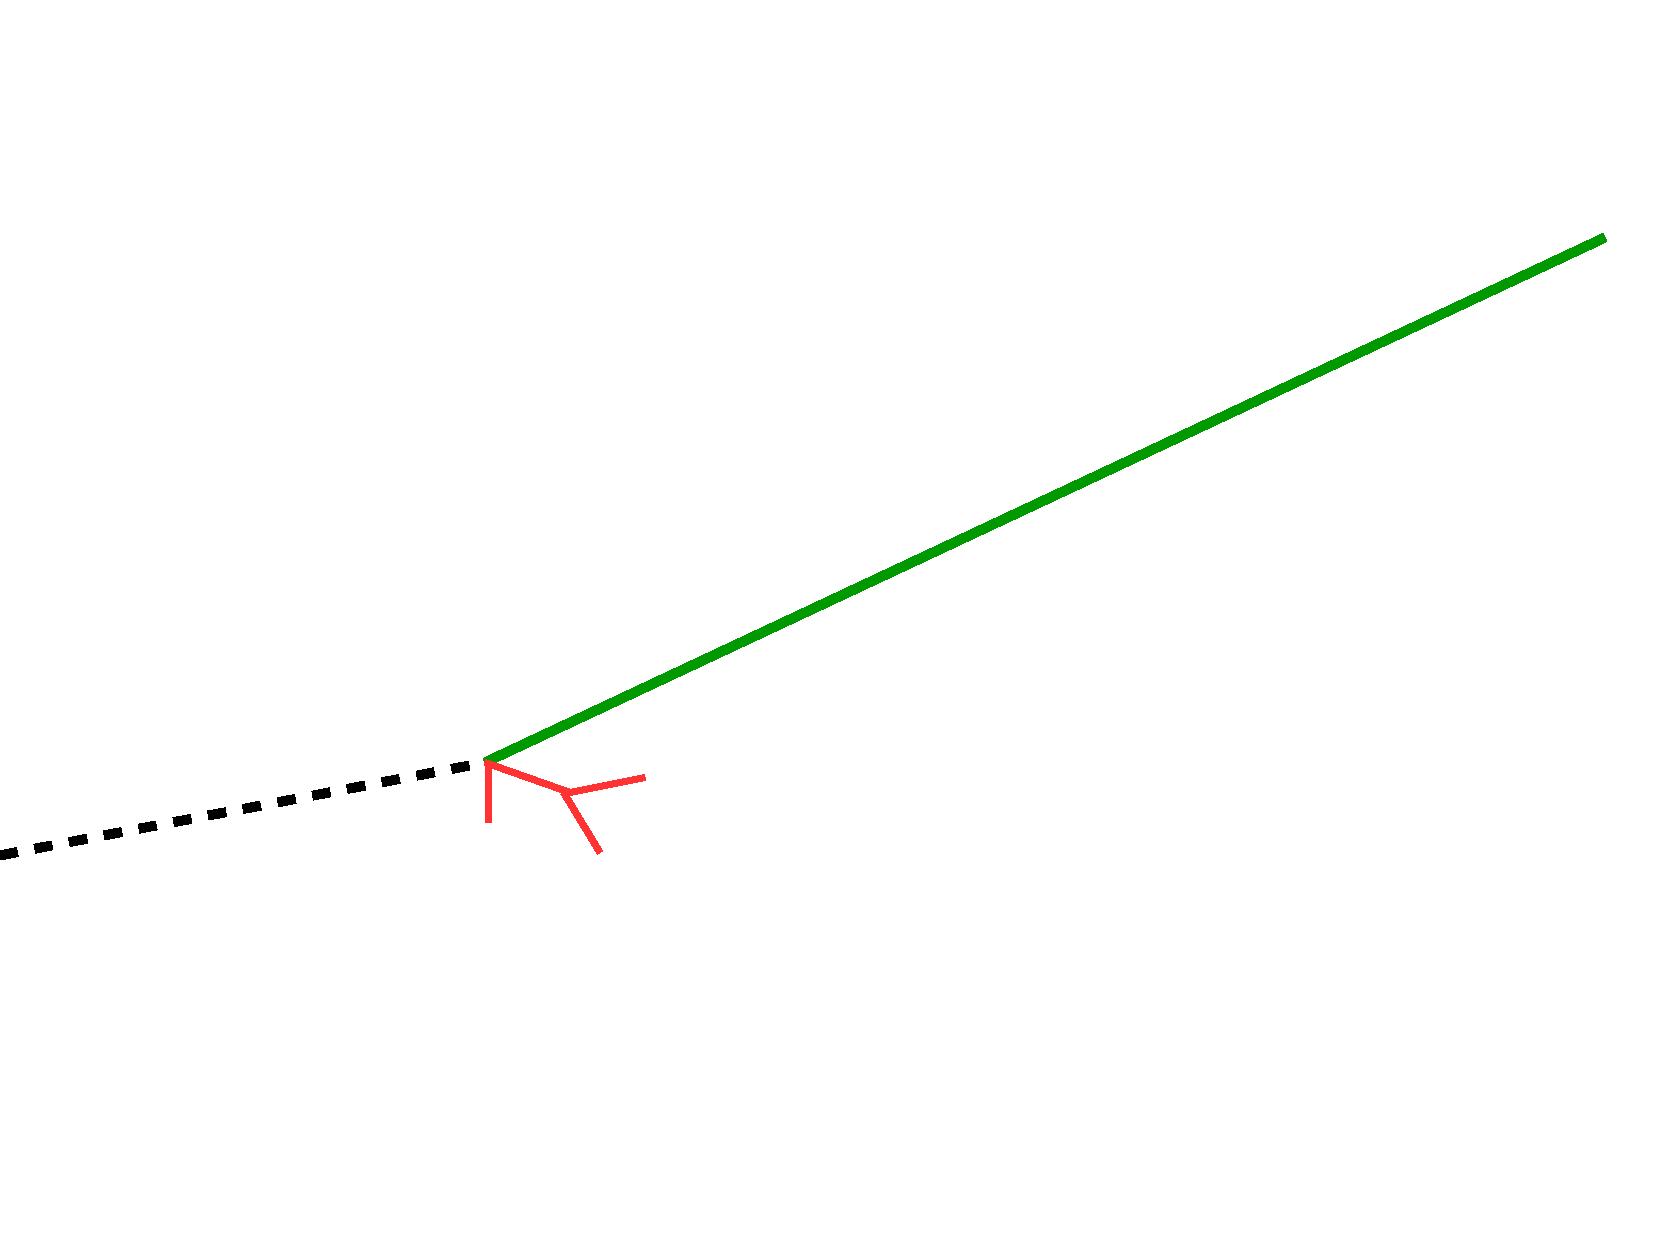
\includegraphics[width=2cm]{figures/neutrinos_properties/interaction_schematics/numu_CC_muon_only.pdf} 
            & $\mu^\pm$ track 
            & Track-only \\

            \cmidrule{2-4} 
            &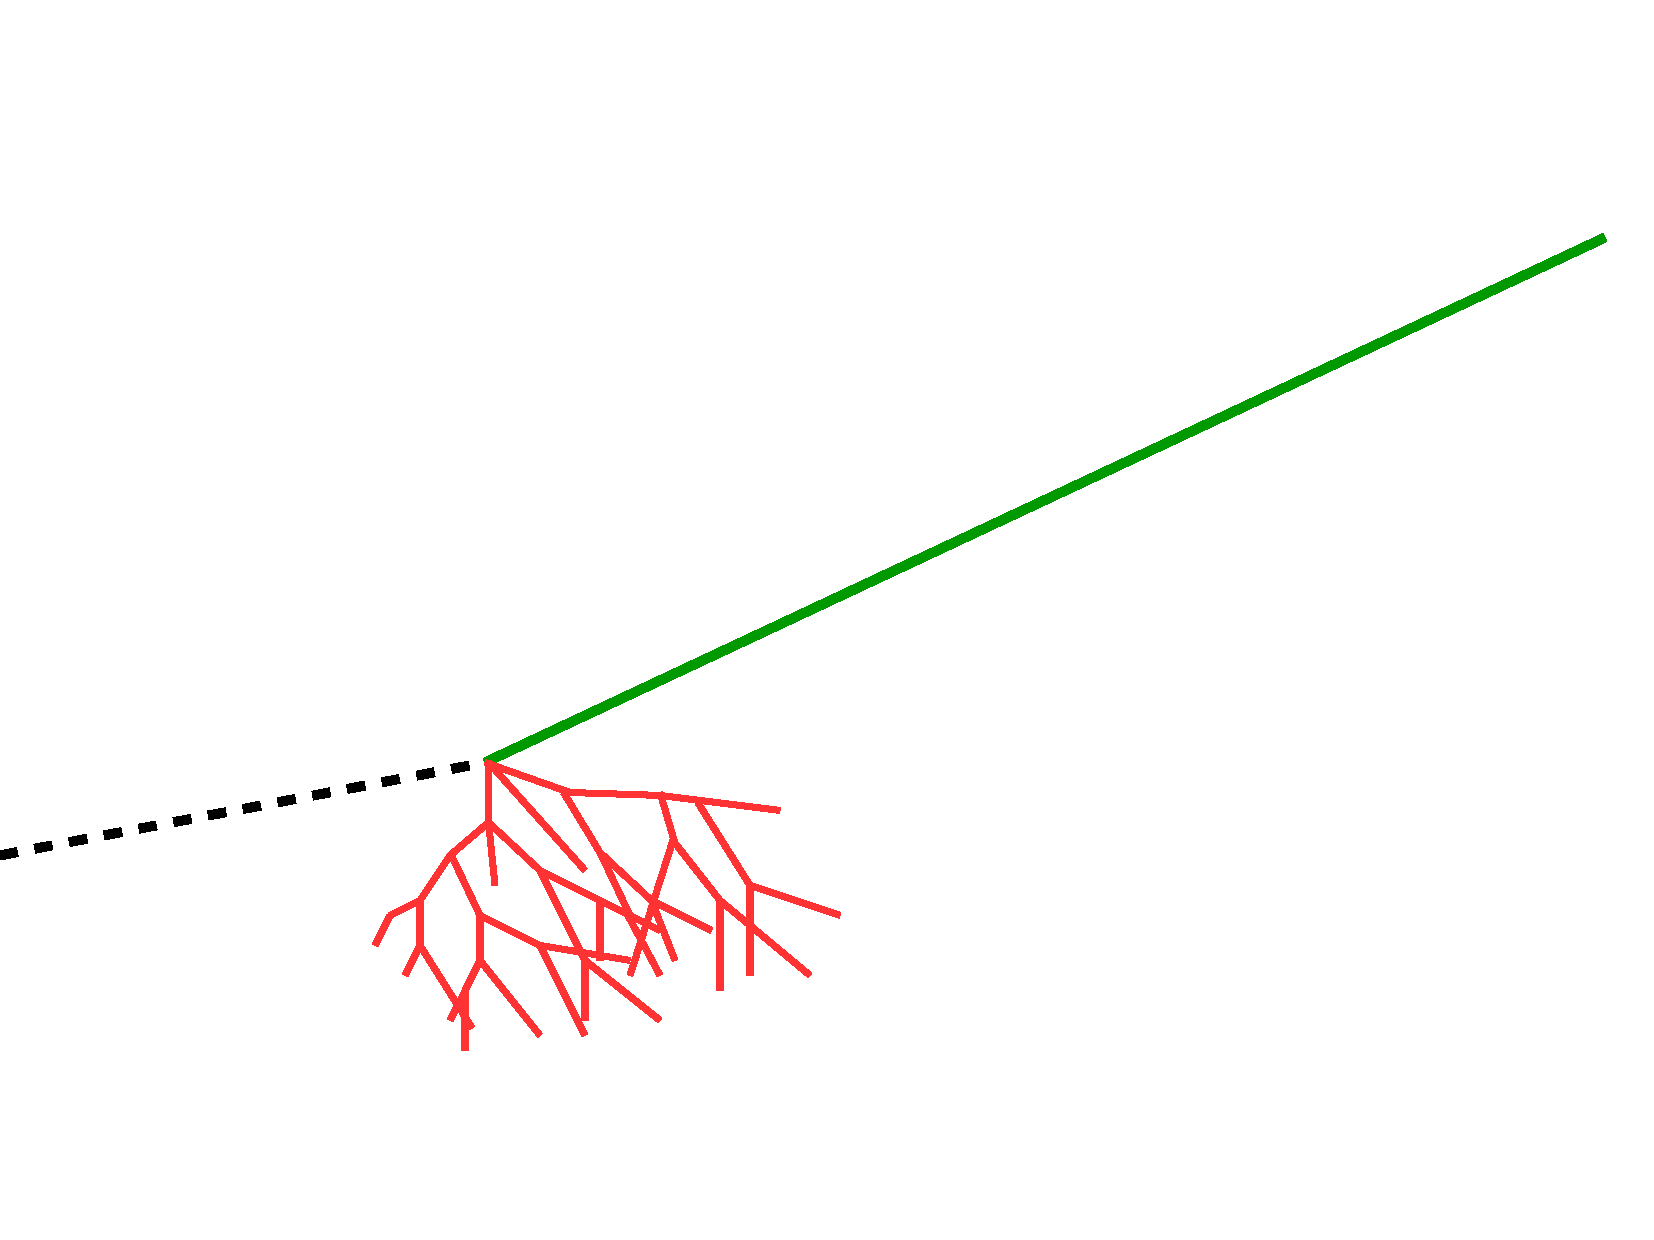
\includegraphics[width=2cm]{figures/neutrinos_properties/interaction_schematics/numu_CC_track_cascade.pdf}  
            & $\mu^\pm$ track and hadrons 
            & \multirow{2}{*}[-1.3em] {Cascade + track} \\

            \cmidrule{1-3}

            \multirow{2}{*}[-1.5em]{CC $\overset{(-)}{\nu_\tau}$ }
            &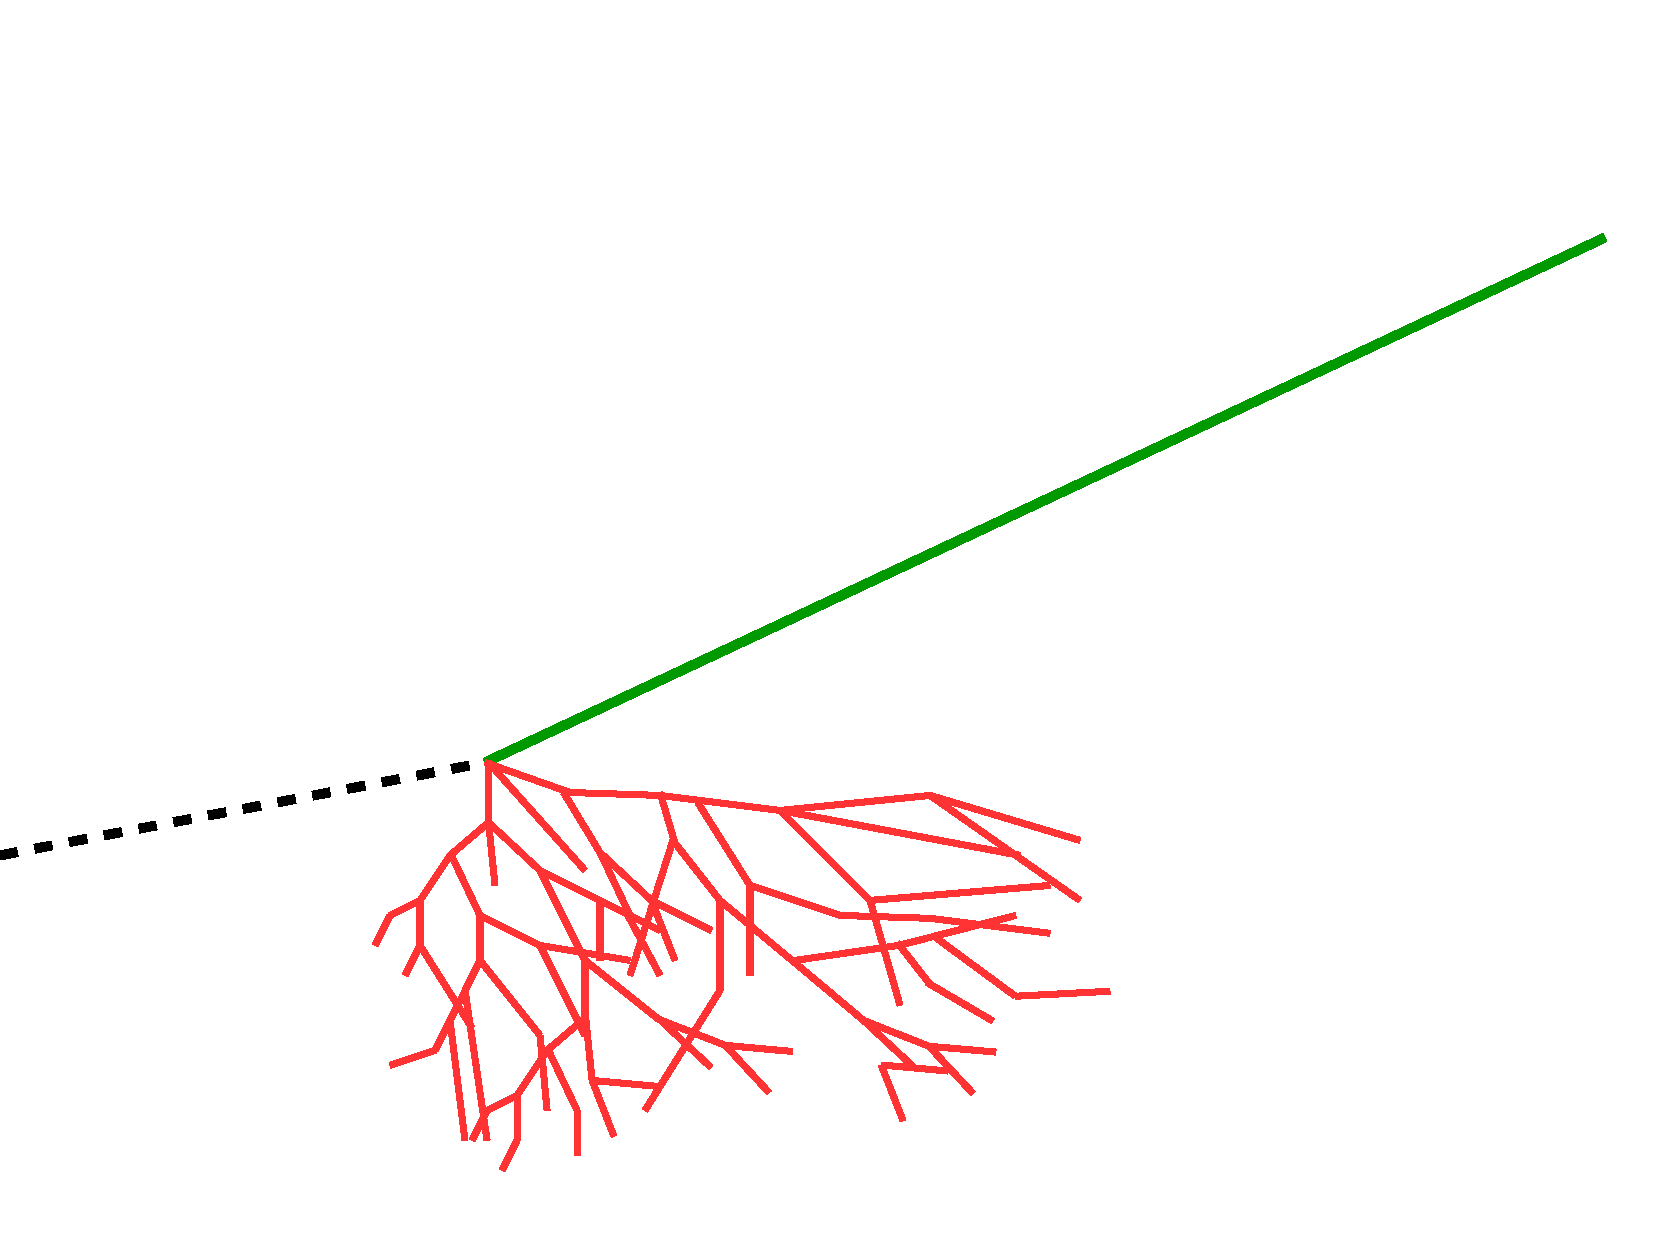
\includegraphics[width=2cm]{figures/neutrinos_properties/interaction_schematics/nutau_CC_track_cascade.pdf} 
            & $\tau^\pm$ decaying into $\mu^\pm$ ($\sim$17\% BR), hadrons 
            & \\

            \cmidrule{2-4}

            & 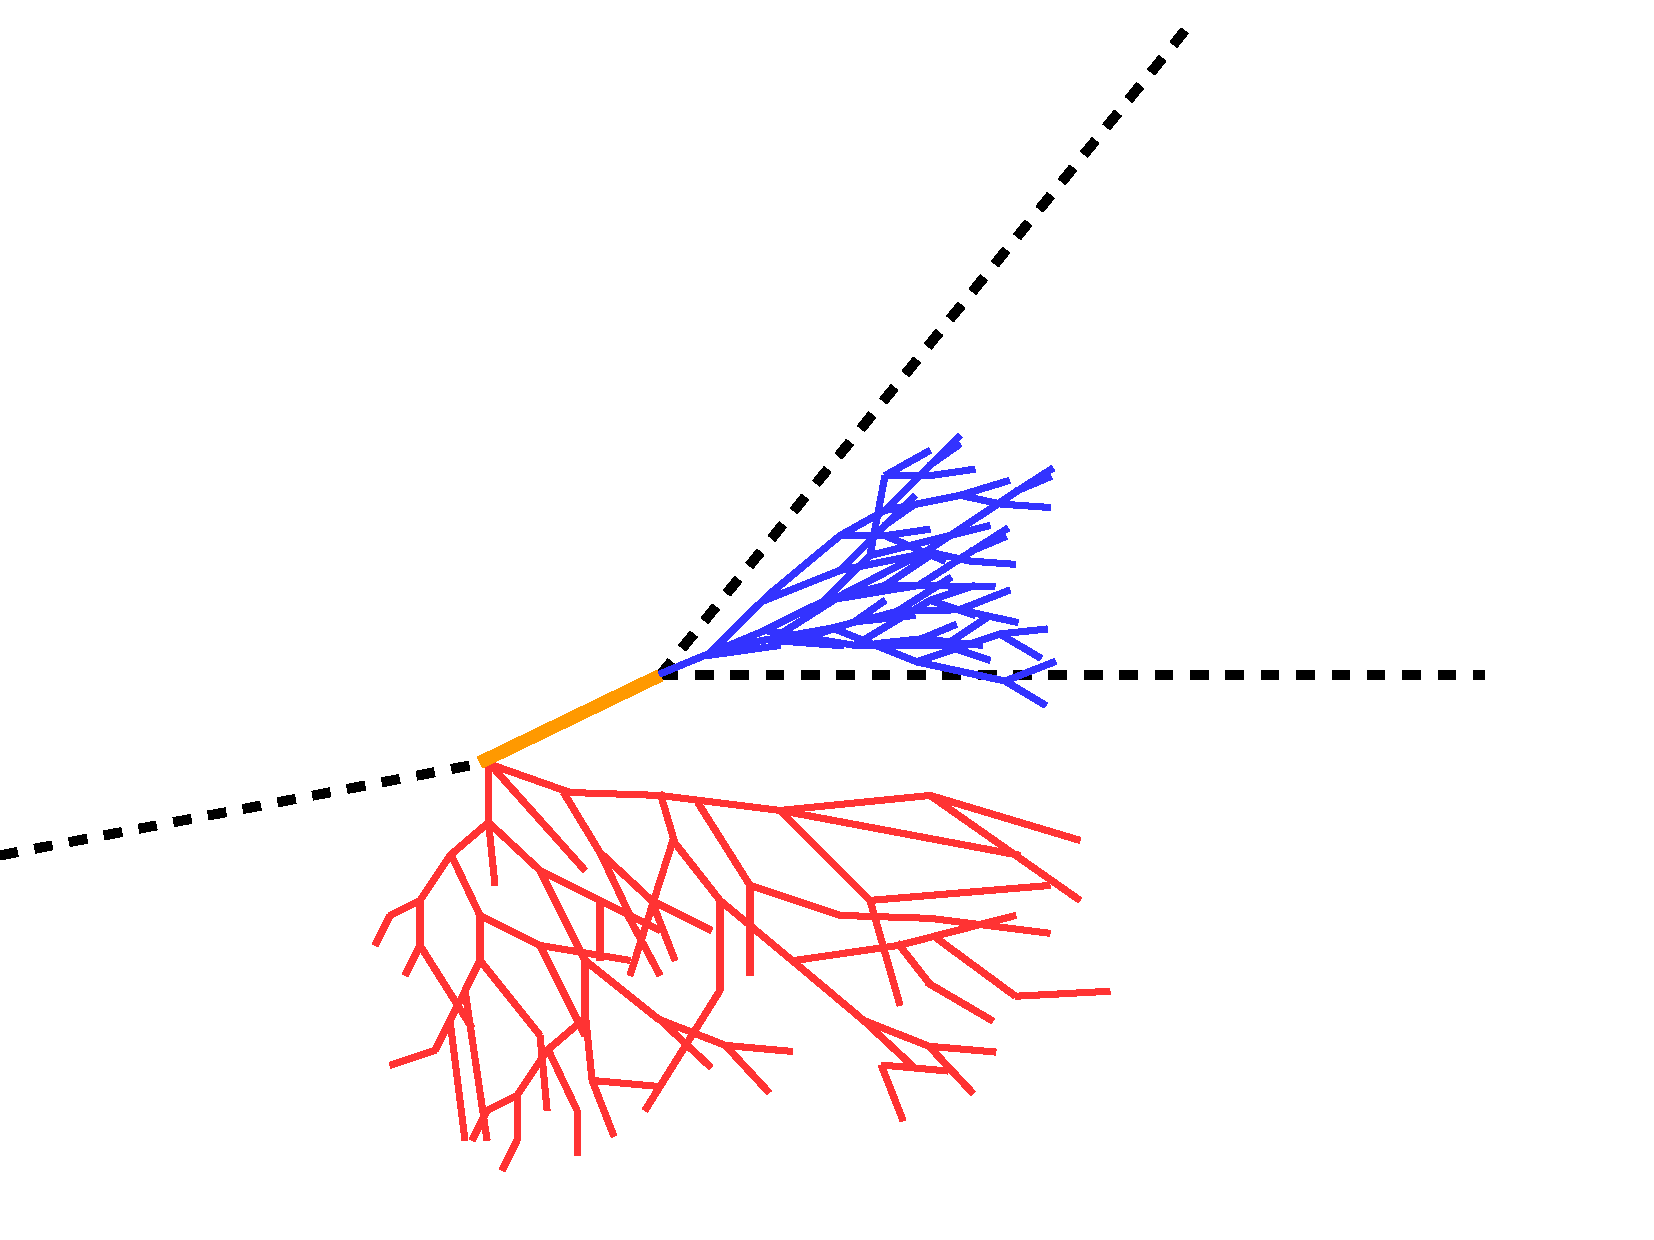
\includegraphics[width=2cm]{figures/neutrinos_properties/interaction_schematics/nutau_CC_cascadeonly.pdf}
            & $\tau^\pm$ decaying into $e^\pm$ or hadrons ($\sim$83\% BR)  
            & \\

            \cmidrule{1-3} CC $\overset{(-)}{\nu_e}$ 
            & 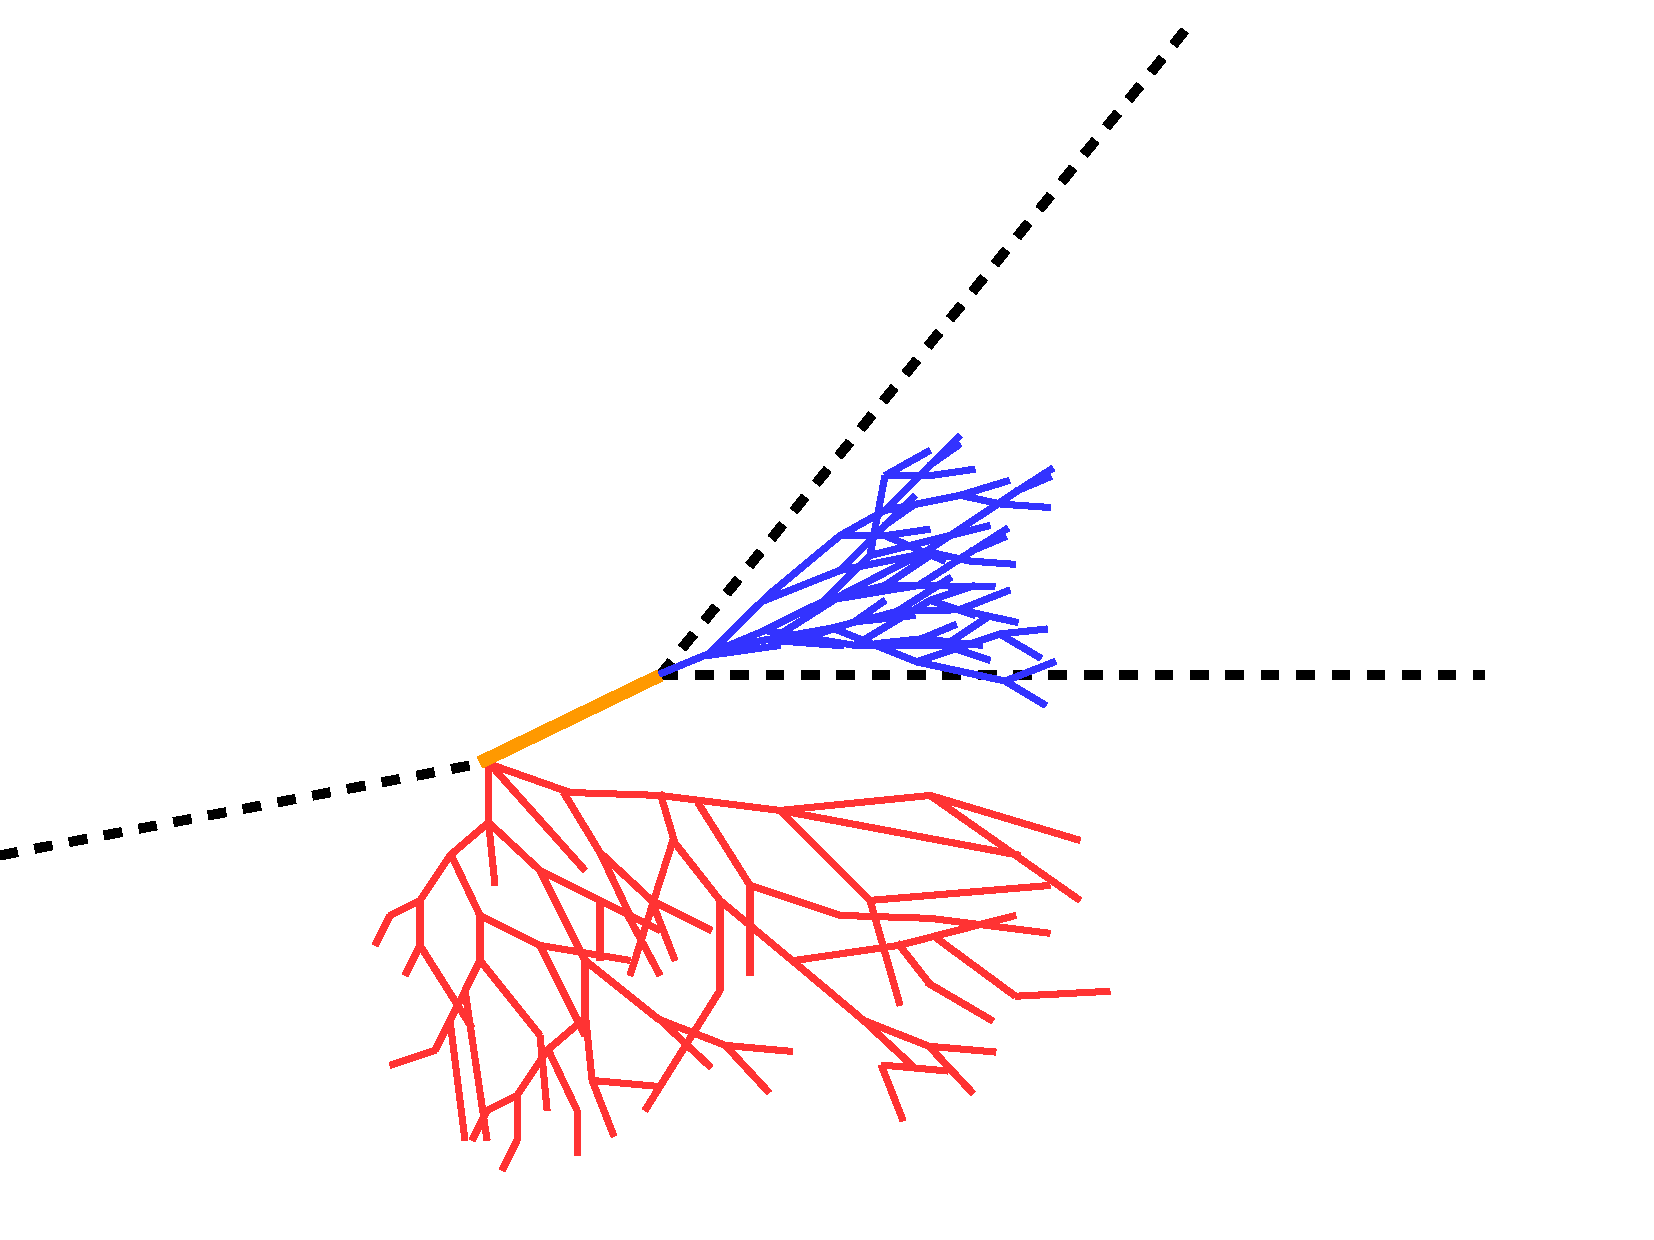
\includegraphics[width=2cm]{figures/neutrinos_properties/interaction_schematics/nue_CC_cascadeonly.pdf}
            & $e^\pm$, hadrons & {Cascade-only} \\

            \cmidrule{1-3}

            NC $\overset{(-)}{\nu_\ell}$ 
            & 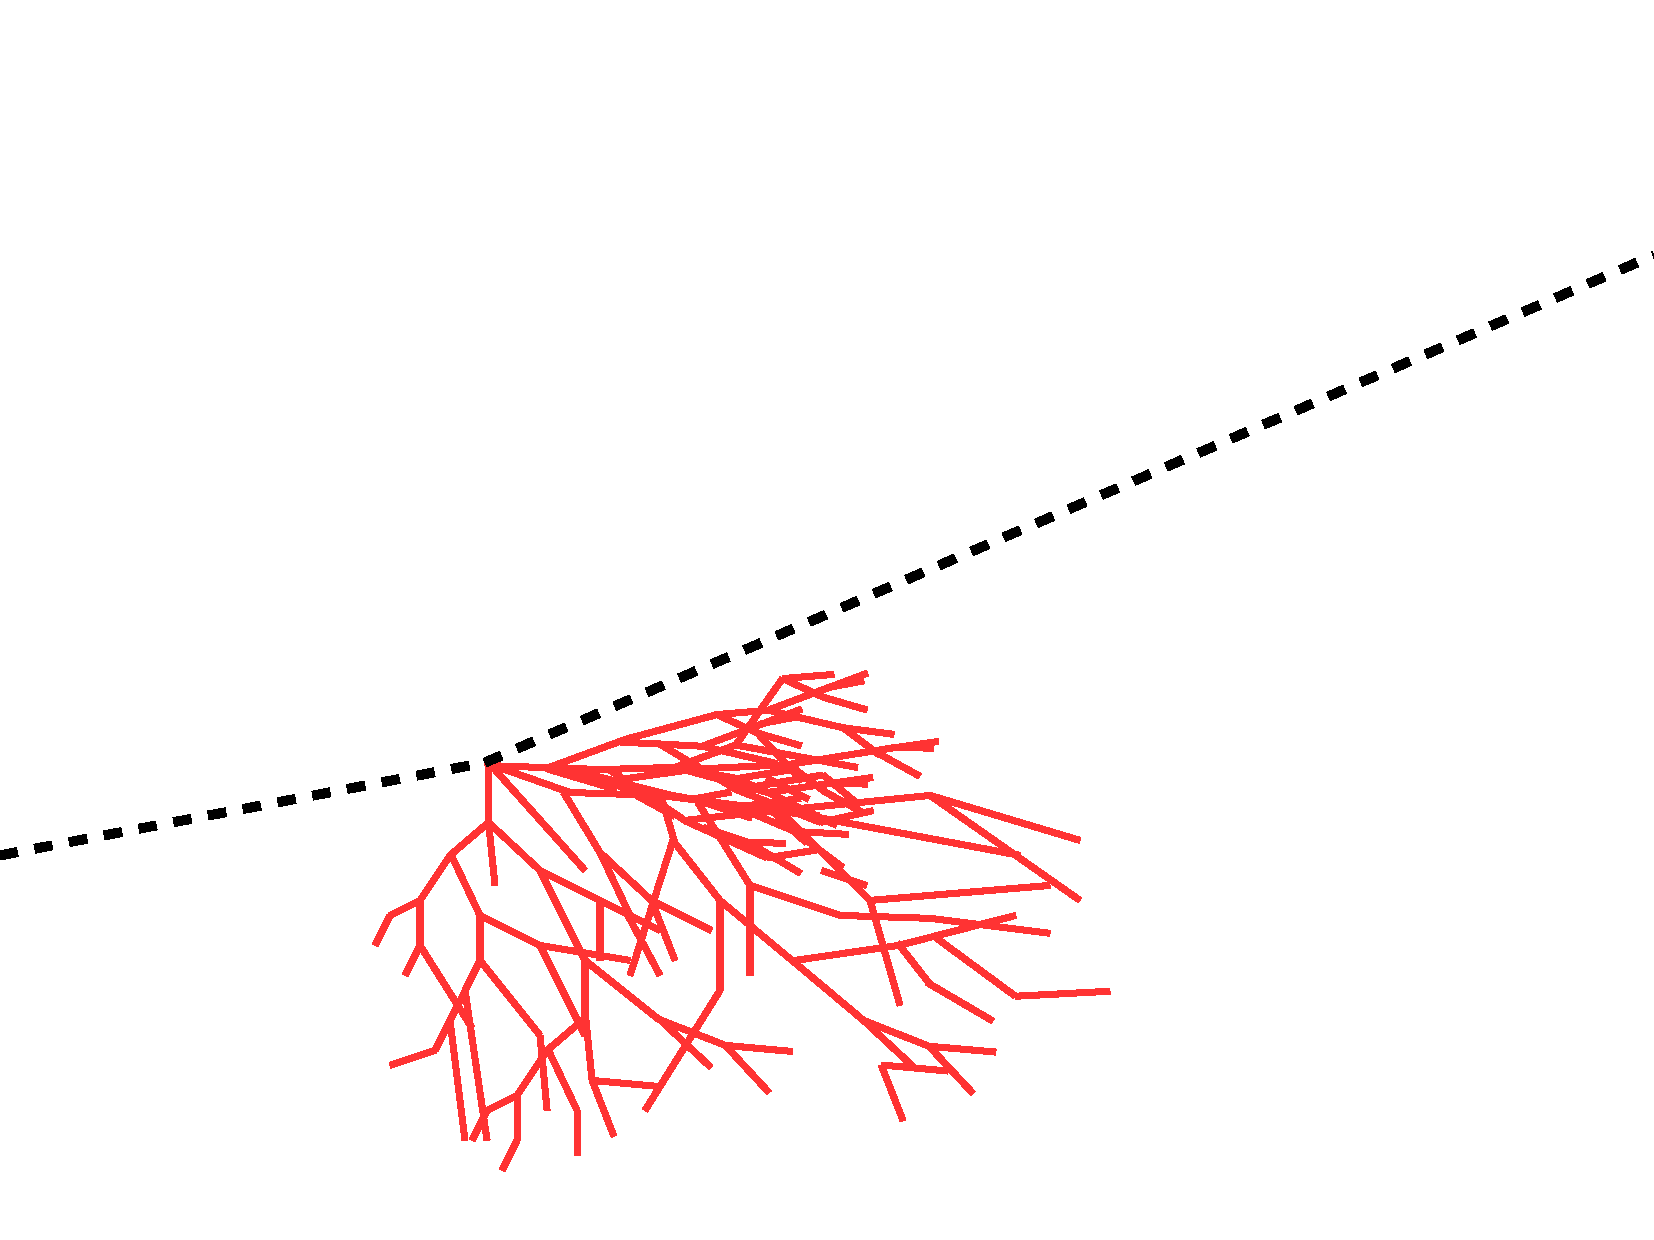
\includegraphics[width=2cm]{figures/neutrinos_properties/interaction_schematics/nuall_NC_cascadeonly.pdf} 
            & hadrons & \\

            \hline
        \end{tabular}
    \end{center}
    \caption[IceCube low energy event signatures and underlying interactions]{IceCube low energy event signatures, their underlying interaction type, and the particles that produce them. Also shown are the secondary particles produced in the interactions. Black dashed lines represent neutrinos, green lines muons, orange line leptons, and blue and red lines are particles in electromagnetic and hadronic cascades, respectively. Adapted from \cite{ATerliuk}.}
    \labtab{interactions_vs_signatures}
\end{table}


\paragraph{Neutrino} interactions are observed as cascades, tracks, or a combination of both, depending on the initial flavor and the interaction type for the specific event.

In $\nu_\mu$ - CC interactions, a muon is produced in addition to a hadronic shower from the breaking nucleus. If the interaction happens outside the detector, but the muon passes through the detector, this will create a track-like signature. The same happens if the interaction happens inside, but the energy transfer to the nucleus is small ($y \approx 0$). At energies relevant for this work, tracks have length at the same order of the distance between DOMs, so they can be observed as such.

If the interaction happens inside the detector and the energy transfer to the hadronic part of the shower is larger, it will create a cascade with a track leaving it. A similar signature is observed after a $\nu_\tau$ - CC interaction, in which a tau is produced that later decays into a muon, with a branching ratio of $\SI{17}{\percent}$.
% occurs if a $\nu_\tau$ - CC interaction happens, creating a tau that decays into a muon (happening with a branching ratio of $\SI{17}{\percent}$).
In those cases the muon usually has a lower energy and the track will be fainter and harder to observe.

The other $\SI{83}{\percent}$ of $\nu_\tau$ - CC interactions produce a tau that decays into an electron or hadrons, leaving a cascade-only signature through the electromagnetic or hadronic shower. All $\nu_e$ - CC interactions also produce pure cascades, since the electron quickly loses its energy in an electromagnetic shower. In all $\nu$ - NC interactions, the produced neutrino escapes and only the hadronic shower is observable. Since the size of the cascades at the energy range of interest is smaller than the spacing of the DOMs, they are approximately observed as point-like, spherical light sources. Even though the light is almost isotropically emitted, some assymmetry remains in the light profile, which can be used to reconstruct the direction of the incoming neutrino.


\paragraph{Atmospheric muons} also produce pure track like signatures, similar to $\nu_\mu$ - CC interactions happening outside the detector. They are one of the main backgrounds for analyses using atmospheric neutrinos and are therefore the target of many filter steps described in \refsec{trigger_and_filter}.


\setchapterstyle{kao}
\setchapterpreamble[u]{\margintoc}

\chapter{Monte Carlo Event Generation and Detector Simulation}
\labch{signal_simulation}

Like many analyses in IceCube, this work is based on MC simulations. The initial step for all particle (non-noise) simulation is the generation of events from selected initial distributions and fluxes. Events are the primary particle and all particles produced in the interaction with the ice. The particles are then propagated through the ice, producing Cherenkov photons, which are propagated further until they reach a DOM or are absorbed in the ice. If they hit a DOM the detector response is simulated. Splitting the simulation steps has the advantage of reusing the outputs of for example the generation step to propagate the particles with different ice model, in order to estimate the systematic impacts of uncertainties of the ice properties. A similar approach can be taken for varying detector response, before starting the event selection. Through this a more efficient (reduced) use of computing resources can be achieved.

The central part of this thesis is the HNL signal simulation itself. Since this is the first search for HNLs with IceCube DeepCore, there was no prior knowledge of the number of events expected per year nor of the performance in terms of reconstruction and classification accuracy. This chapter describes the first HNL event generation developed for IceCube DeepCore. Two avenues of generation were pursued in parallel. A collection of model-independent samples is explained in \refsec{model_independent_simulation}. They were used for performance benchmarking and for cross-checks to validate the physically accurate, model-dependent event generation, which is described in \refsec{model_specific_simulation}. The event generation for SM background events is briefly described in \refsec{sm_event_generation}, followed by the detector response simulation in \refsec{detector_simulation}.


\section{Model-Independent Heavy Neutral Lepton Event Generation} \labsec{model_independent_simulation}

To investigate the potential of IceCube to detect HNLs by identifying the unique double-cascade morphology explained in \refsec{double_cascade_morphology}, a model-independent double-cascade generator was developed, where the kinematics of each cascade can be controlled directly. Using this generator, several simulation samples were produced to investigate the performance of IceCube DeepCore to detect low-energy double-cascades, dependent on their properties. All samples are produced using a collection of custom generator functions~\cite{cascade_generator_functions} that place two EM cascade vertices with variable energy and direction at configurable locations in the detector.


\subsection{Simplistic Samples} \labsec{simplistic_samples}

To investigate the best-case and the worst-case double-cascade event scenarios, two samples are produced in the DeepCore volume: straight up-going events ($\cos(\theta)=-1$) that are centered on a string and horizontal events ($\cos(\theta)=0$). The first sample is used to investigate one of the most promising scenarios to detect a double-cascade, where both cascade centers are located on a DeepCore string and the directions are directly up-going. One of the DeepCore strings was randomly chosen as the $x$-$y$ coordinate for this sample. As already mentioned in \refsec{deepcore}, DeepCore strings have higher quantum efficiency DOMs and a denser vertical spacing, making them better to detect low-energy events that produce little light. To produce the events, the $x,y$ position of the cascades is fixed to the center of the string while the $z$ positions are each sampled uniformly along the axis of the string. Note that this will therefore not produce a uniform length distribution between the cascades. The positions are defined in the IceCube coordinate system that was introduced in \refsec{icecube}. The energies are sampled uniformly between \SIrange[range-phrase={~and~}]{0.0}{60.0}{\gev}, to generously cover the region where $\nu_\mu\rightarrow\nu_\tau$ appearance is maximized. The time of the lower cascade is set to $t_0=\SI{0.0}{\nano\second}$ and for the upper one to $t_1=L/c$, assuming the HNL travels at the speed of light, $c$. \reffig{simplified_gen_distris} shows the resulting energy distributions and the decay length distribution, where it can be seen how the uniform cascade energies sum into a non-uniform total energy, and the decay length distribution is also non-uniform due to the uniform $z$ sampling of both cascades, which sets the distance between them.

\begin{figure*}[h]
    \centering
    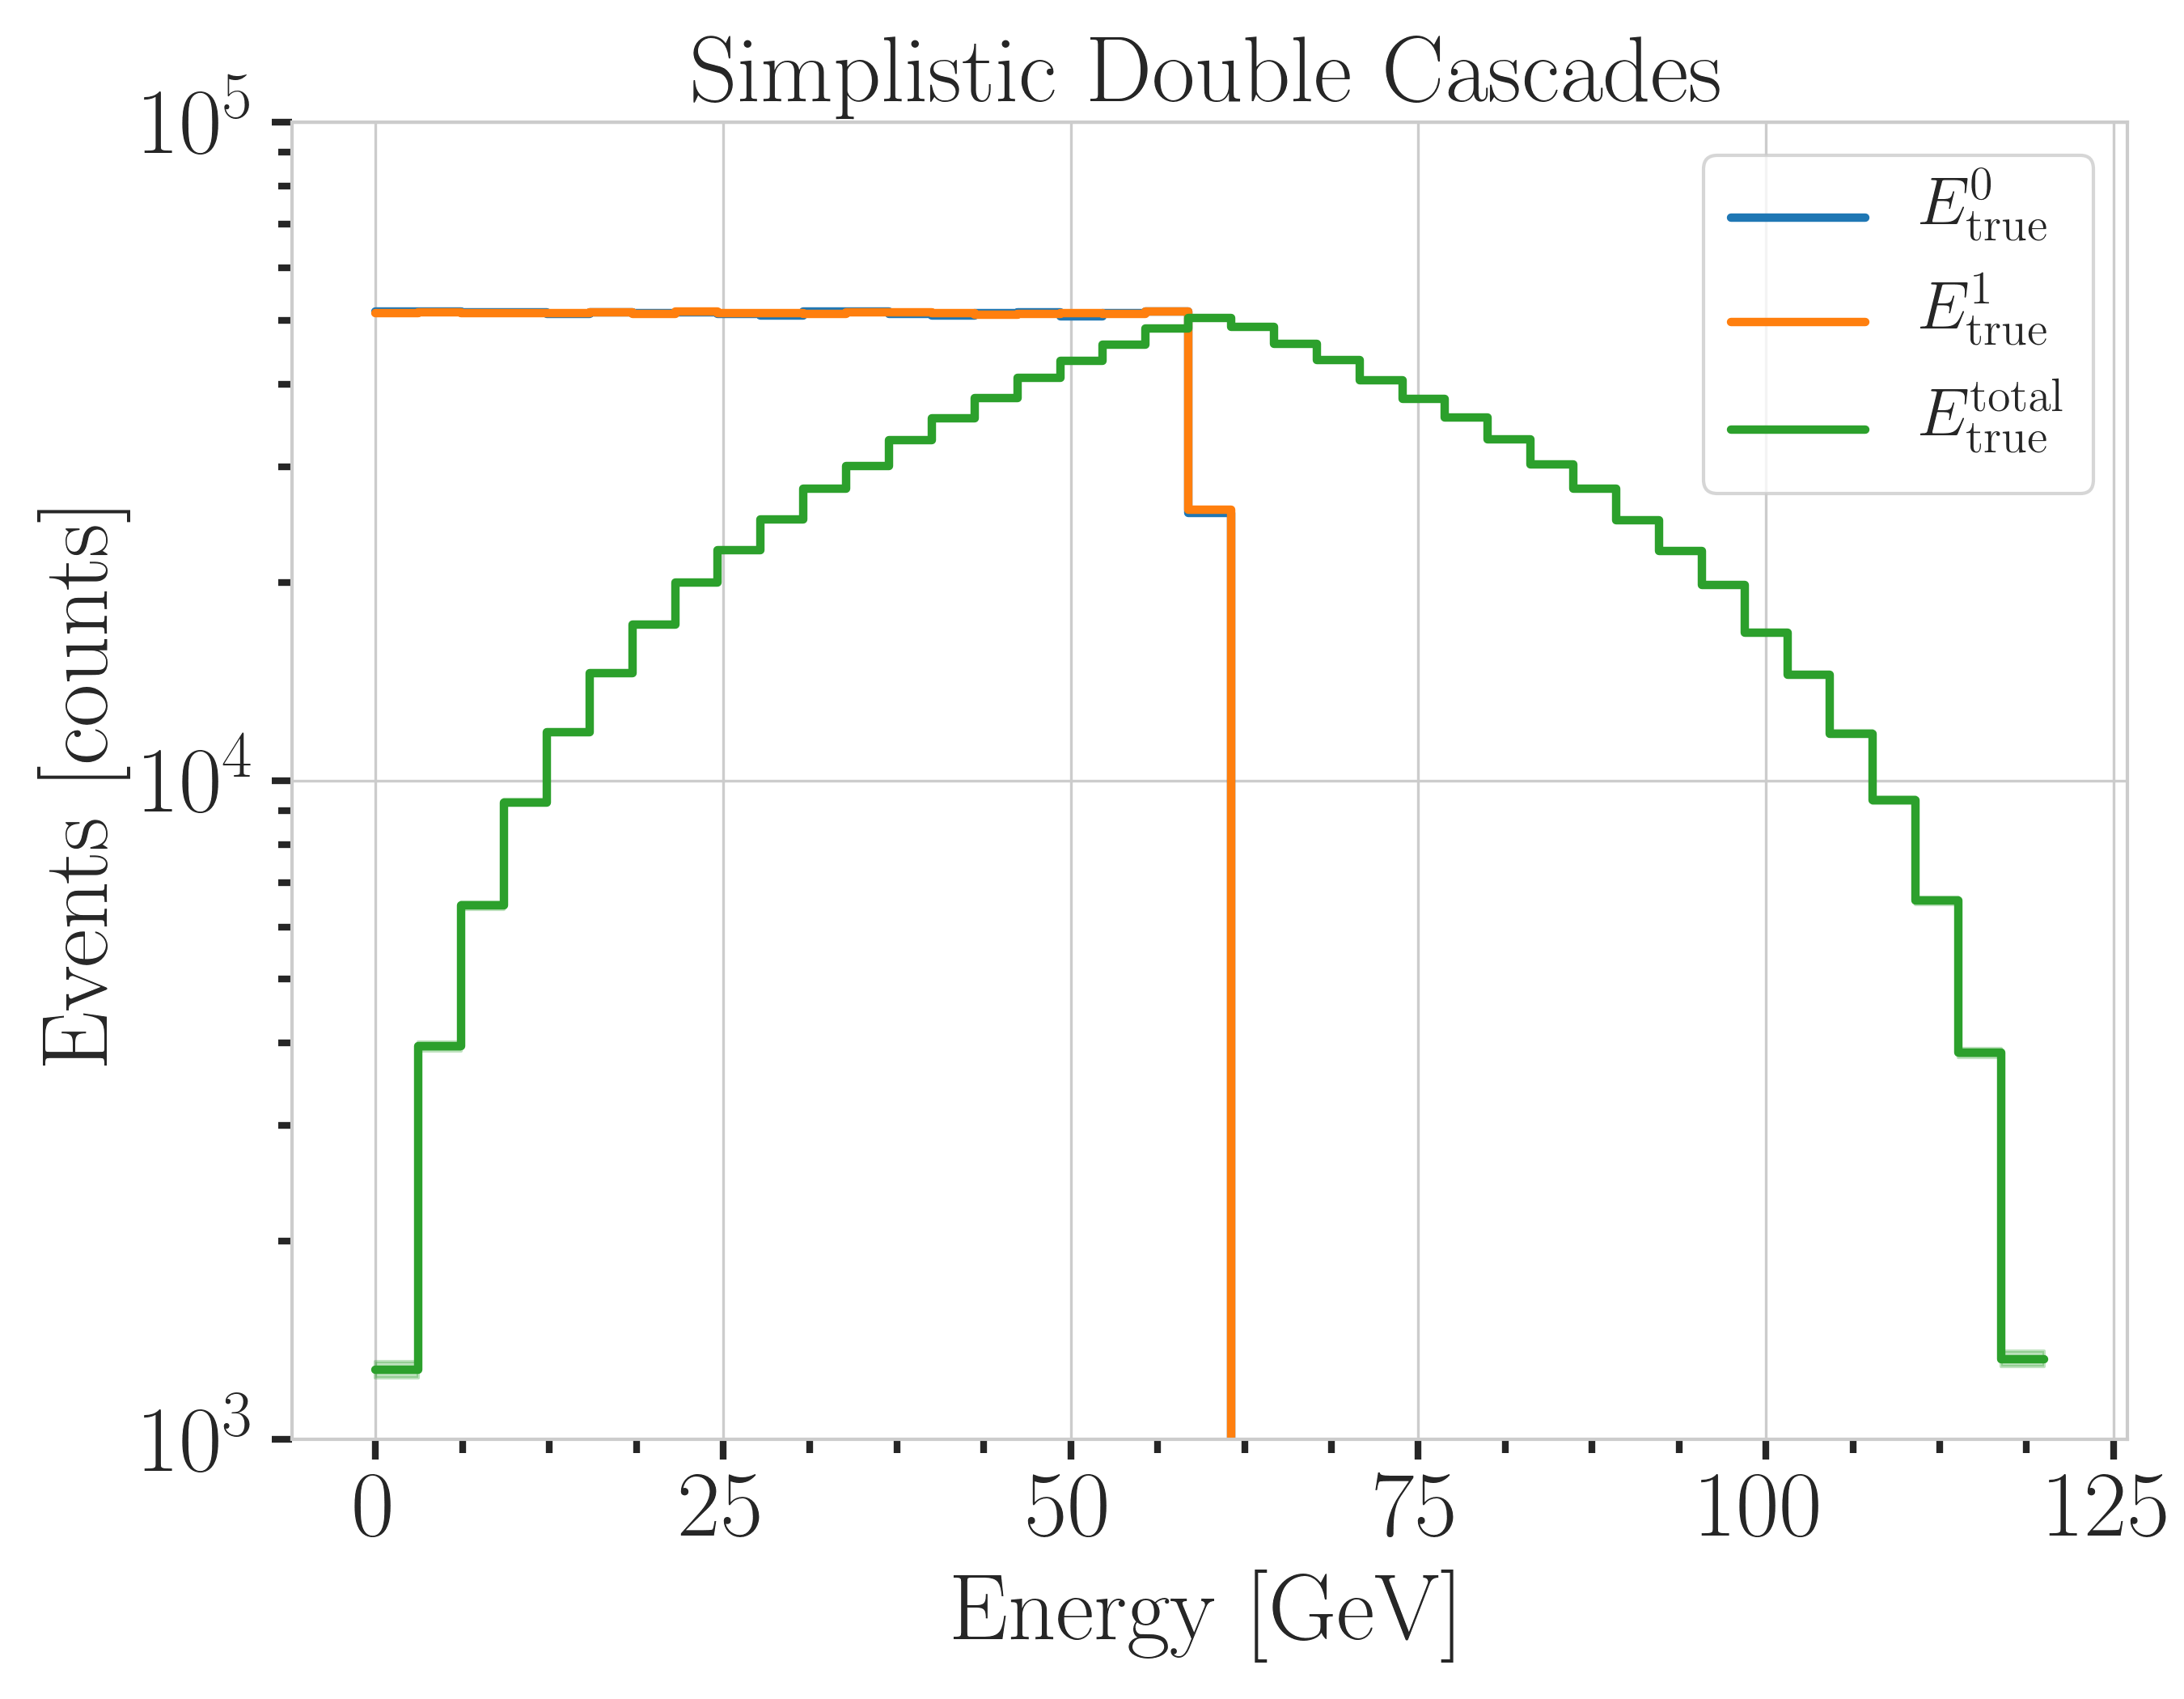
\includegraphics[width=.49\linewidth]{figures/model_independent_simulation/gen_level/simplistic_1_d_distr_all_energies.png}
    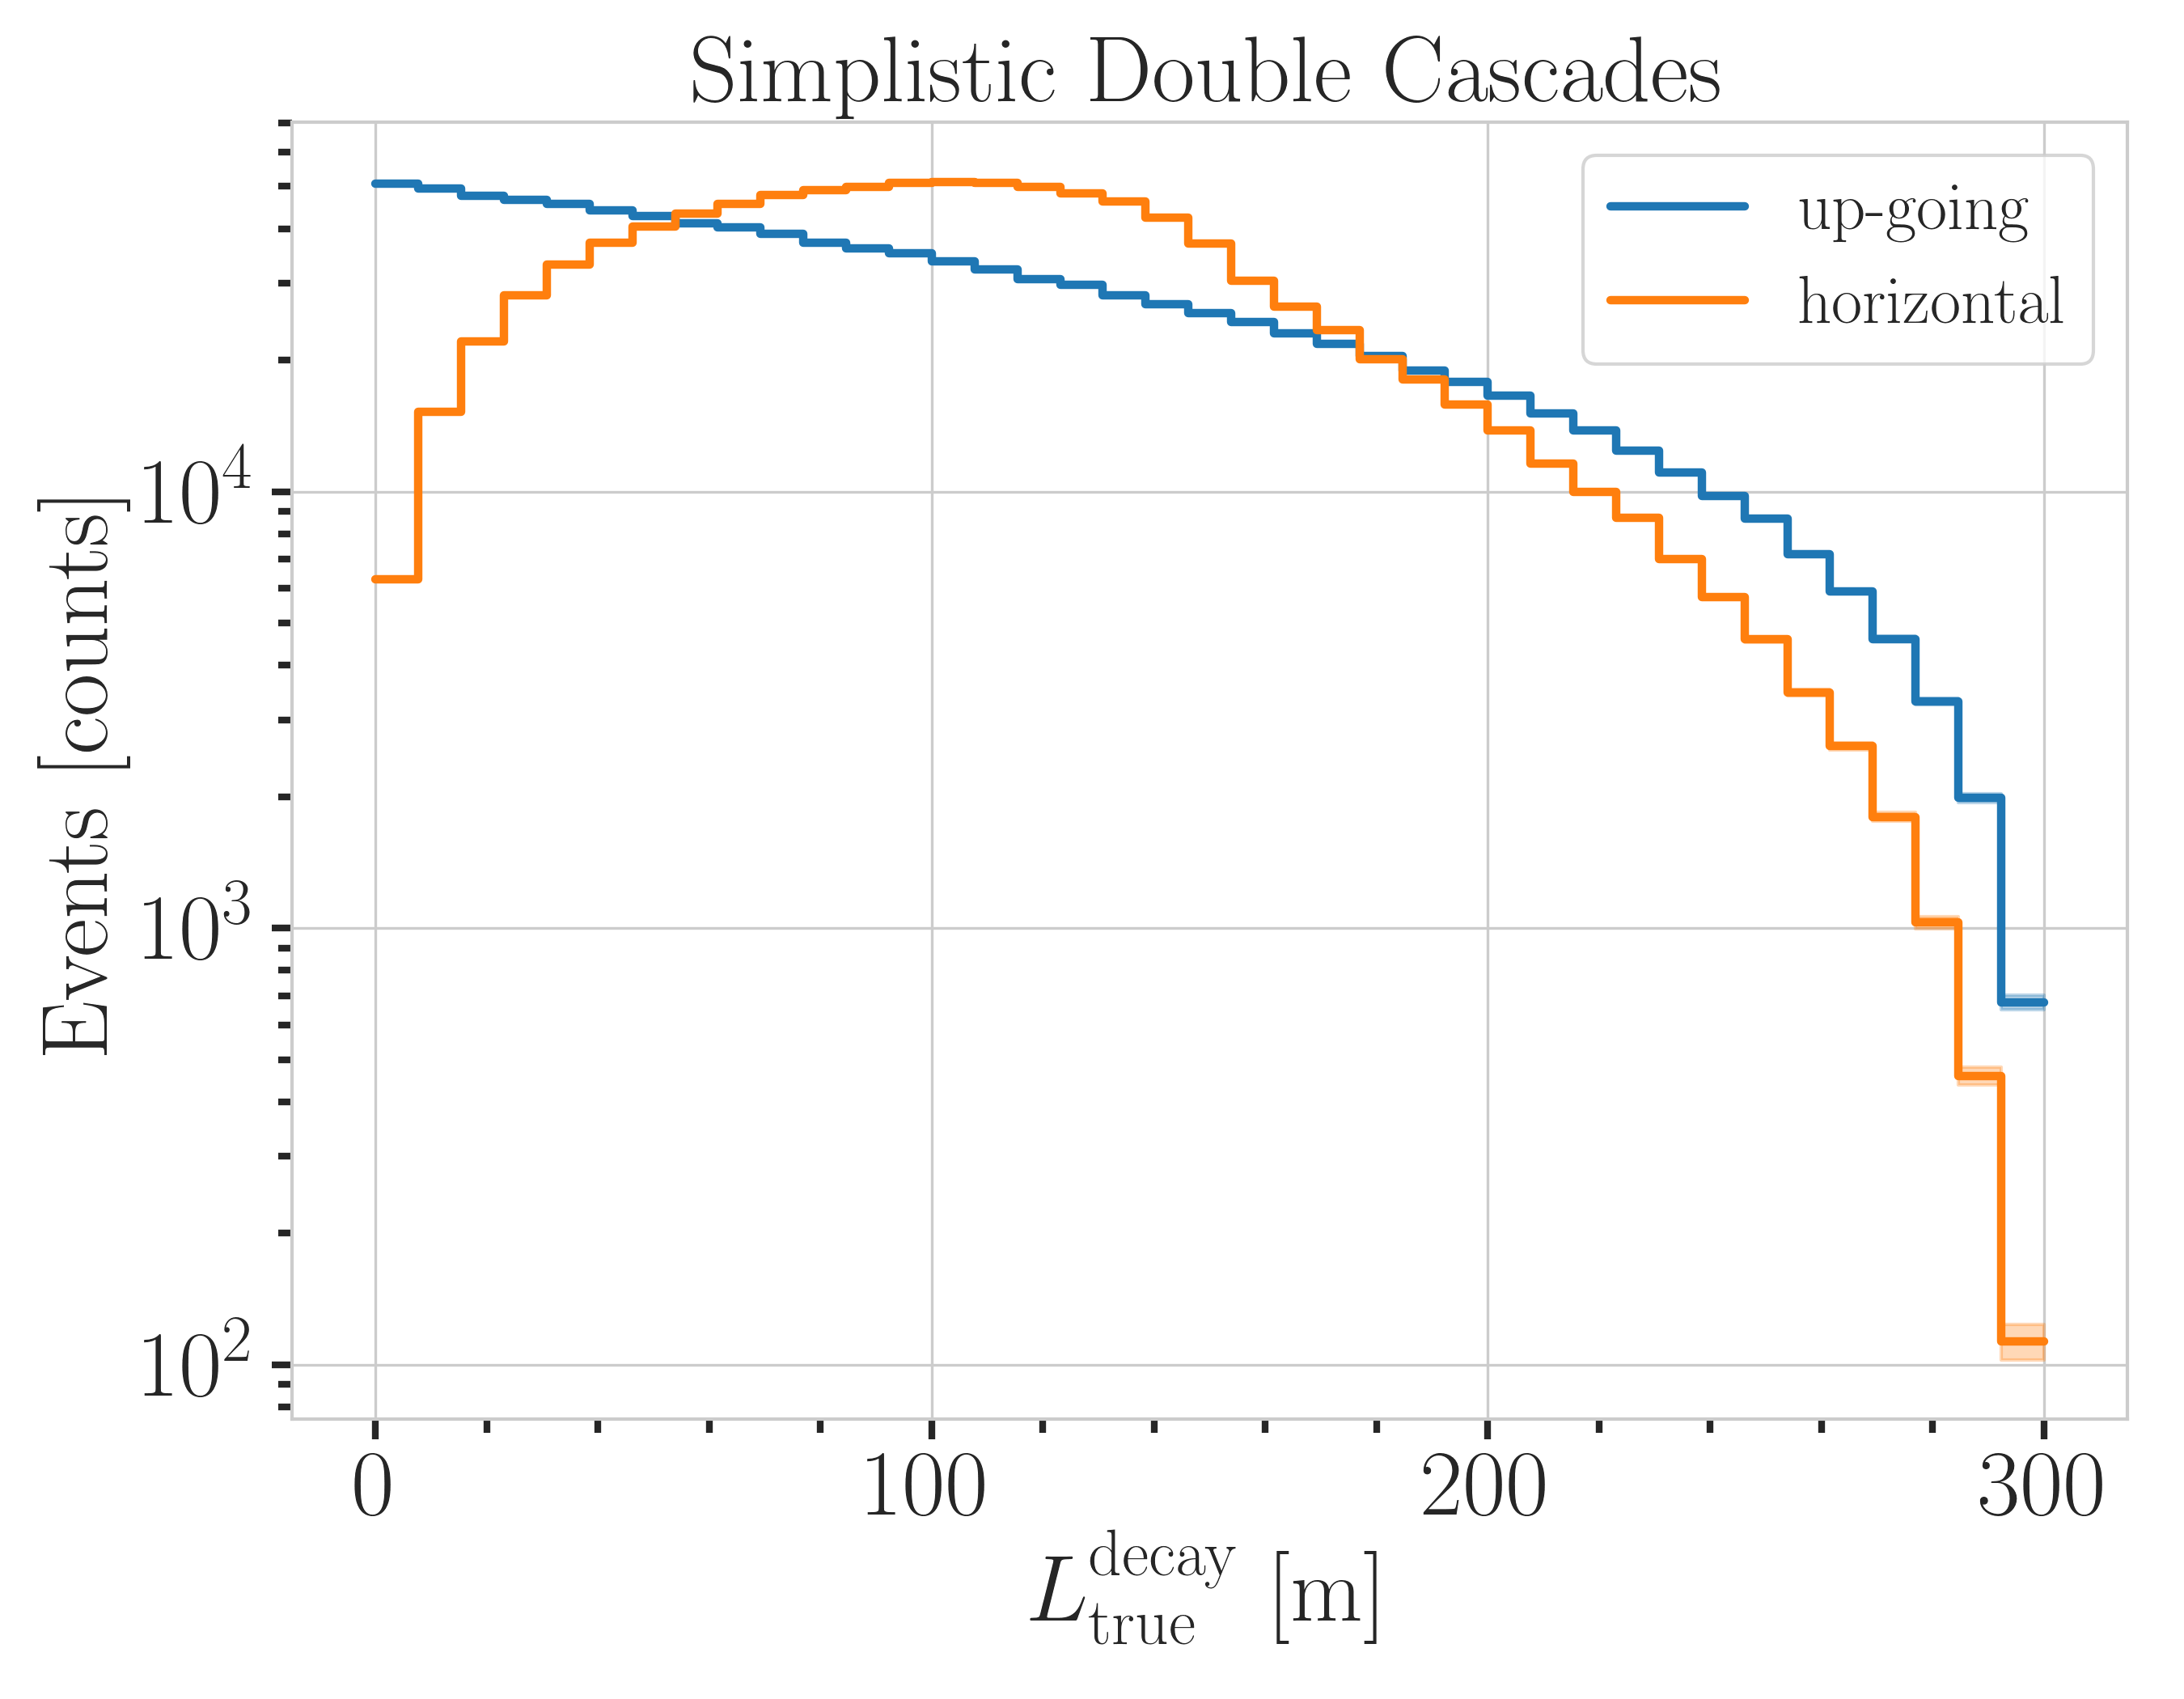
\includegraphics[width=.49\linewidth]{figures/model_independent_simulation/gen_level/simplistic_1_d_distr_true_decay_length.png}
    \caption[Simplified model-independent simulation generation level distributions]{Generation level distributions of the simplistic simulation samples. Cascade and total energies (left) and decay lengths (right) of both samples are shown. The energy distributions are identical for both samples and therefore only shown once.}
    \labfig{simplified_gen_distris}
\end{figure*}

The second sample is used to investigate the worst-case scenario of horizontal events, where the spacing between DOMs is much larger. The cascades are placed uniformly on a circle with radius of $r=\SI{150}{\meter}$ centered in DeepCore at the depth of $z=\SI{-330}{\meter}$. The direction is always horizontal and azimuth is defined by the connecting vector of both cascade positions. The energies are again sampled uniformly between \SIrange[range-phrase={~and~}]{0.0}{60.0}{\gev}. The specific sampling distributions/values for the cascades are listed in \reftab{hnl_simplified_sampling_distributions}, for both samples, and for completeness, all distributions are shown in \reffig{realistic_gen_distris_appendix}.

\begin{table}[h]
    \small
        \begin{tabular}{ llll }
        \hline\hline
        \textbf{Sample} & \textbf{Variable} & \textbf{Distribution} & \textbf{Range/Value} \\
        \hline\hline
        \multicolumn{2}{l}{Up-going} && \\
        \hline
        & energy & uniform & \SIrange{0.0}{60.0}{\gev} \\
        & zenith & fixed & \SI{180.0}{\degree} \\
        & azimuth & fixed & \SI{0.0}{\degree} \\
        & $x,y$ position & fixed & (41.6, 35.49)\,\si{\metre} \\
        & $z$ position & uniform & \SIrange{-480.0}{-180.0}{\metre} \\
        \hline
        \multicolumn{2}{l}{Horizontal} && \\ 
        \hline
        & energy & uniform & \SIrange{0.0}{60.0}{\gev} \\
        & zenith & fixed & \SI{90.0}{\degree} \\
        & azimuth & uniform & \SIrange{0.0}{360.0}{\degree} \\
        & $x,y$ position & uniform (circle) & $c$=(46.29, -34.88)\,\si{\metre}, $r$=\SI{150.0}{\metre} \\
        & $z$ position & fixed & \SI{-330.0}{\metre} \\
        \hline
        \end{tabular}
    \caption[Simplified model-independent simulation sampling distributions]{Generation level sampling distributions and ranges/values of up-going and horizontal model-independent sample.}
    \labtab{hnl_simplified_sampling_distributions}
\end{table}


\subsection{Realistic Sample} \labsec{realistic_sample}

To thoroughly investigate the potential of IceCube DeepCore to detect double-cascade events, a more realistic simulation sample is produced that aims to be as close as possible to the expected signal simulation, while still allowing additional freedom to control the double-cascade kinematics. This sample is particularly useful for validating the model-dependent HNL simulation described in \refsec{model_specific_simulation}.

For this purpose the total energy is sampled from an $E^{-2}$ power law, mimicking the energy spectrum of the primary neutrinos as stated in \refsec{neutrino_generation}. The total energy is divided into two parts, by assigning a fraction between \SIrange[range-phrase={~and~}]{0}{100}{\percent} to one cascade and the remaining part to the other cascade. This is a generic approximation of the realistic process, and chosen such that the whole sample covers various cases of energy distributions between the two cascades. The decay length is sampled from an exponential distribution, as expected for a particle decay. The resulting energy distributions and the decay length distribution are shown in \reffig{realistic_gen_distris}, where it can be seen that the individual cascade energies can be very small, due to splitting the total energy, and the decay lengths spans across several orders of magnitude.

\begin{figure*}[h]
    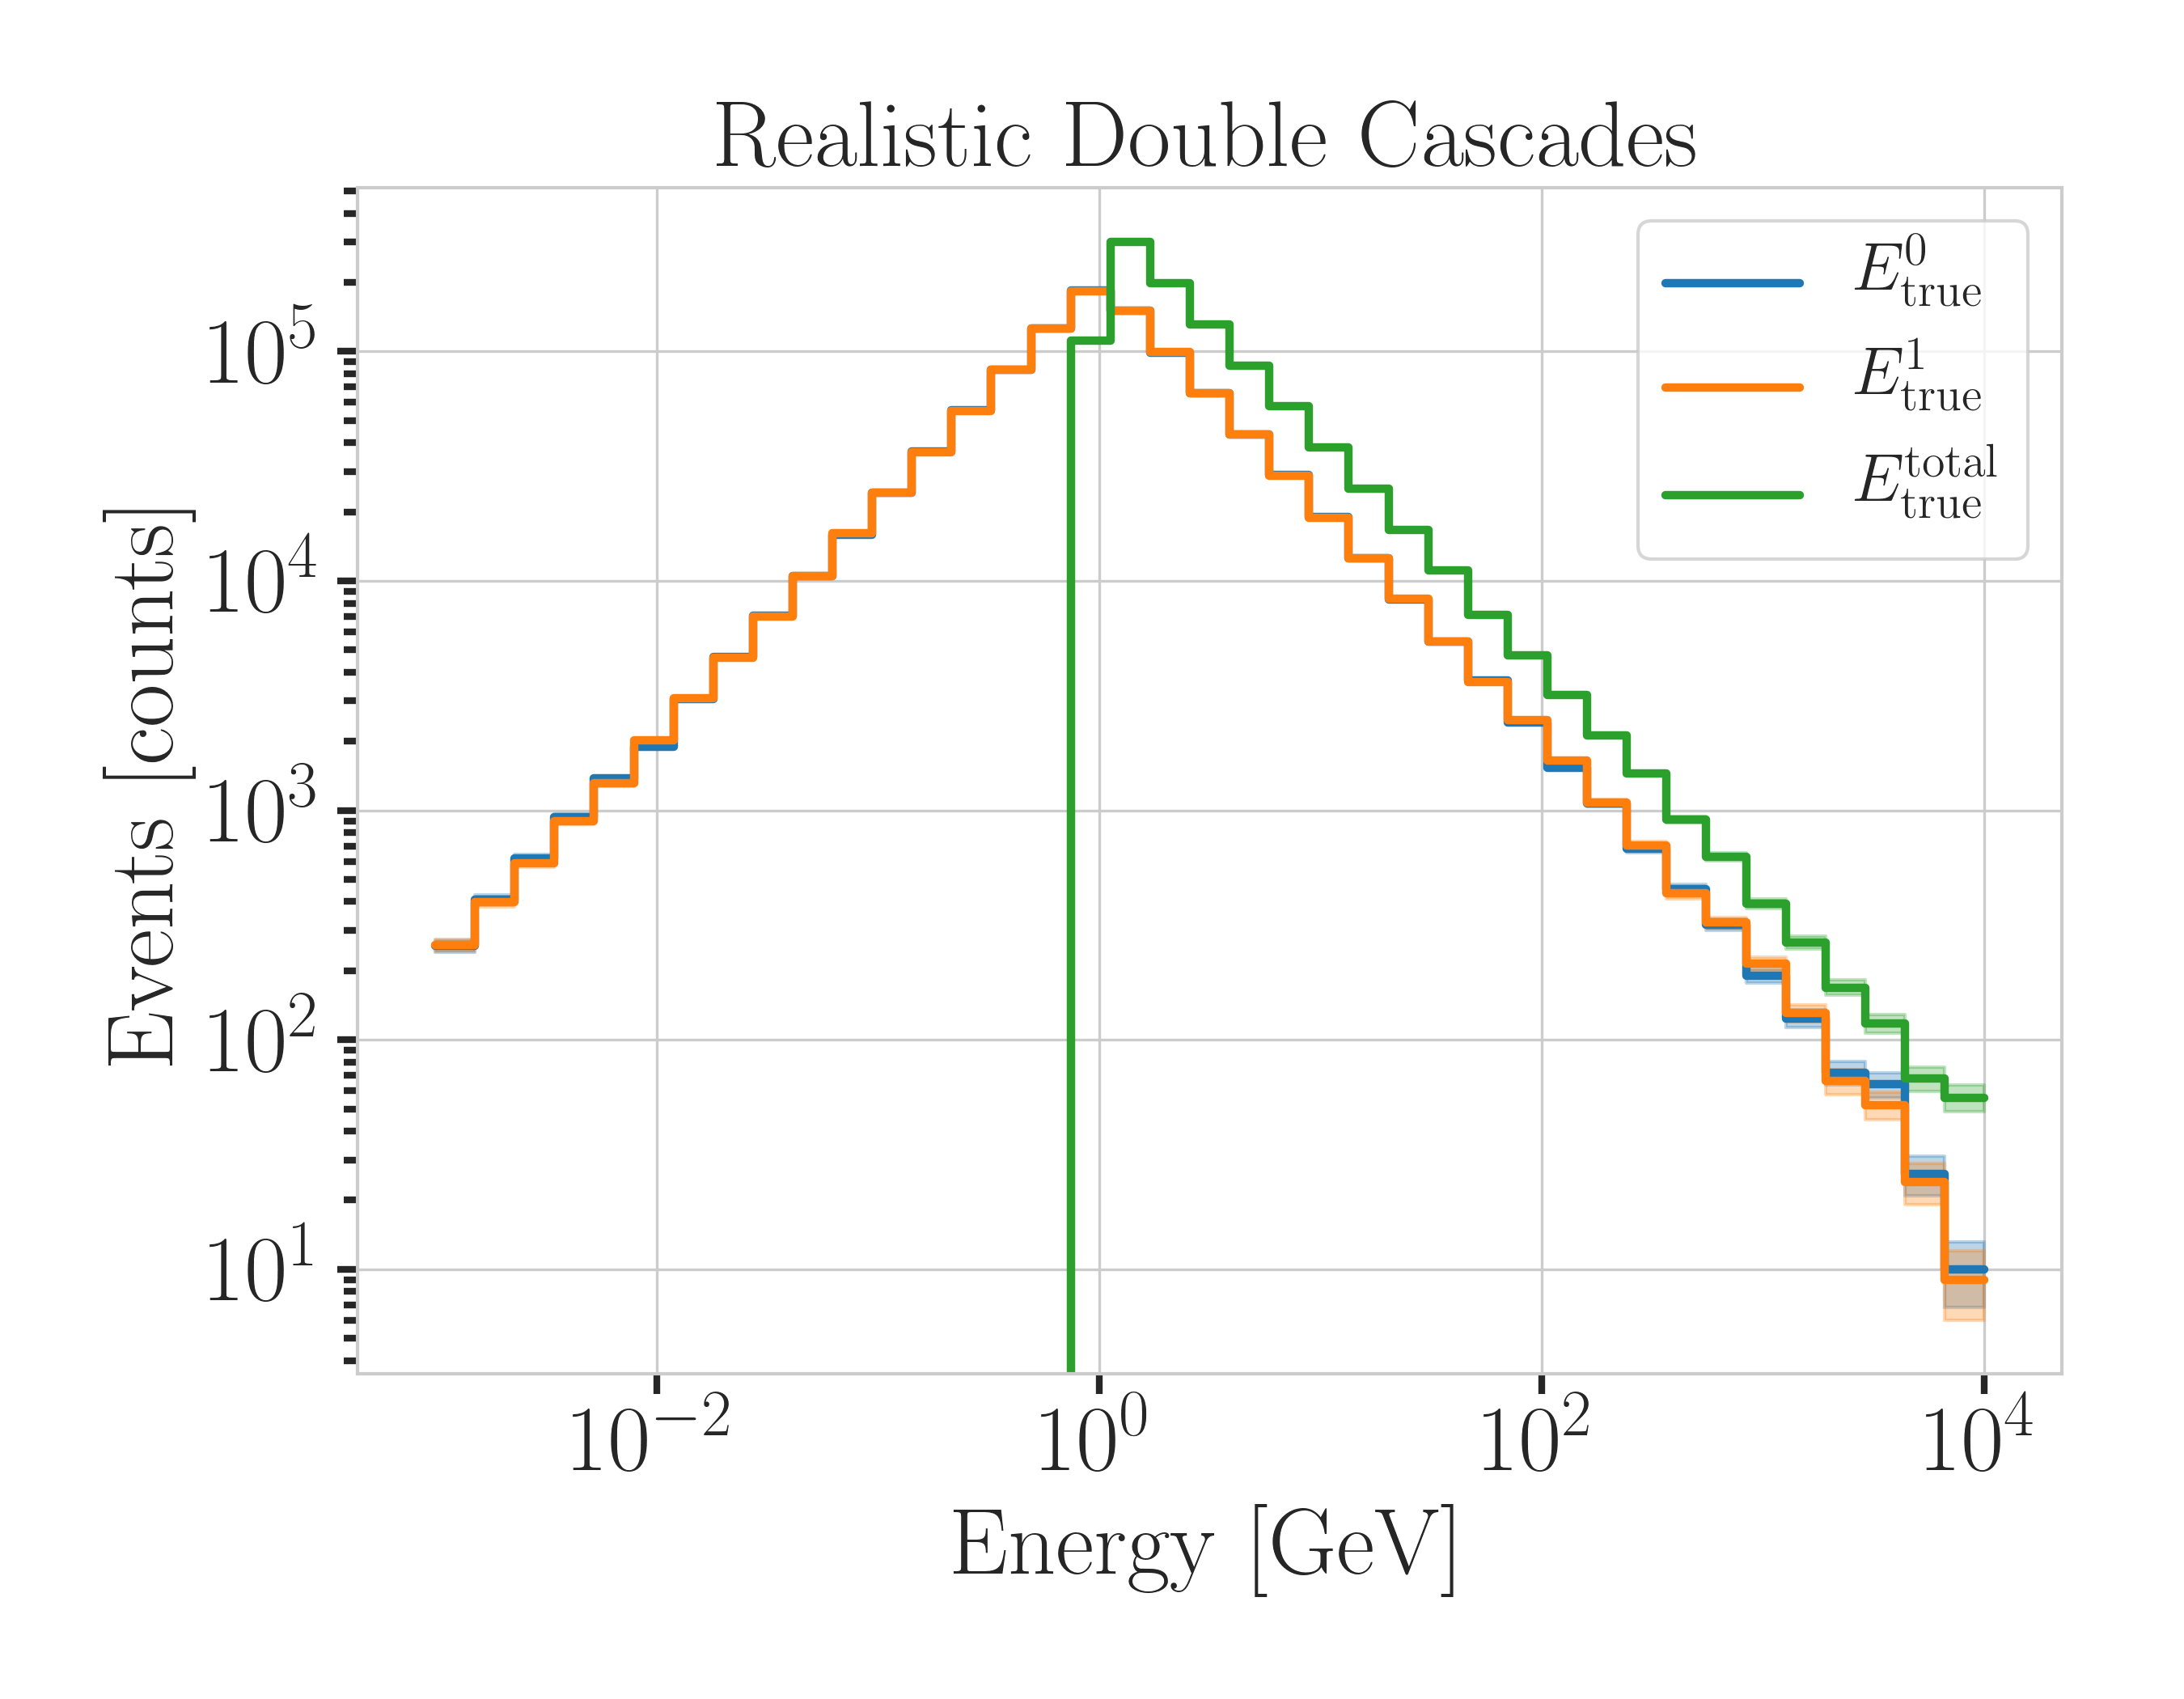
\includegraphics[width=.49\linewidth]{figures/model_independent_simulation/gen_level/194603_gen_level_1_d_distr_all_energies.png}
    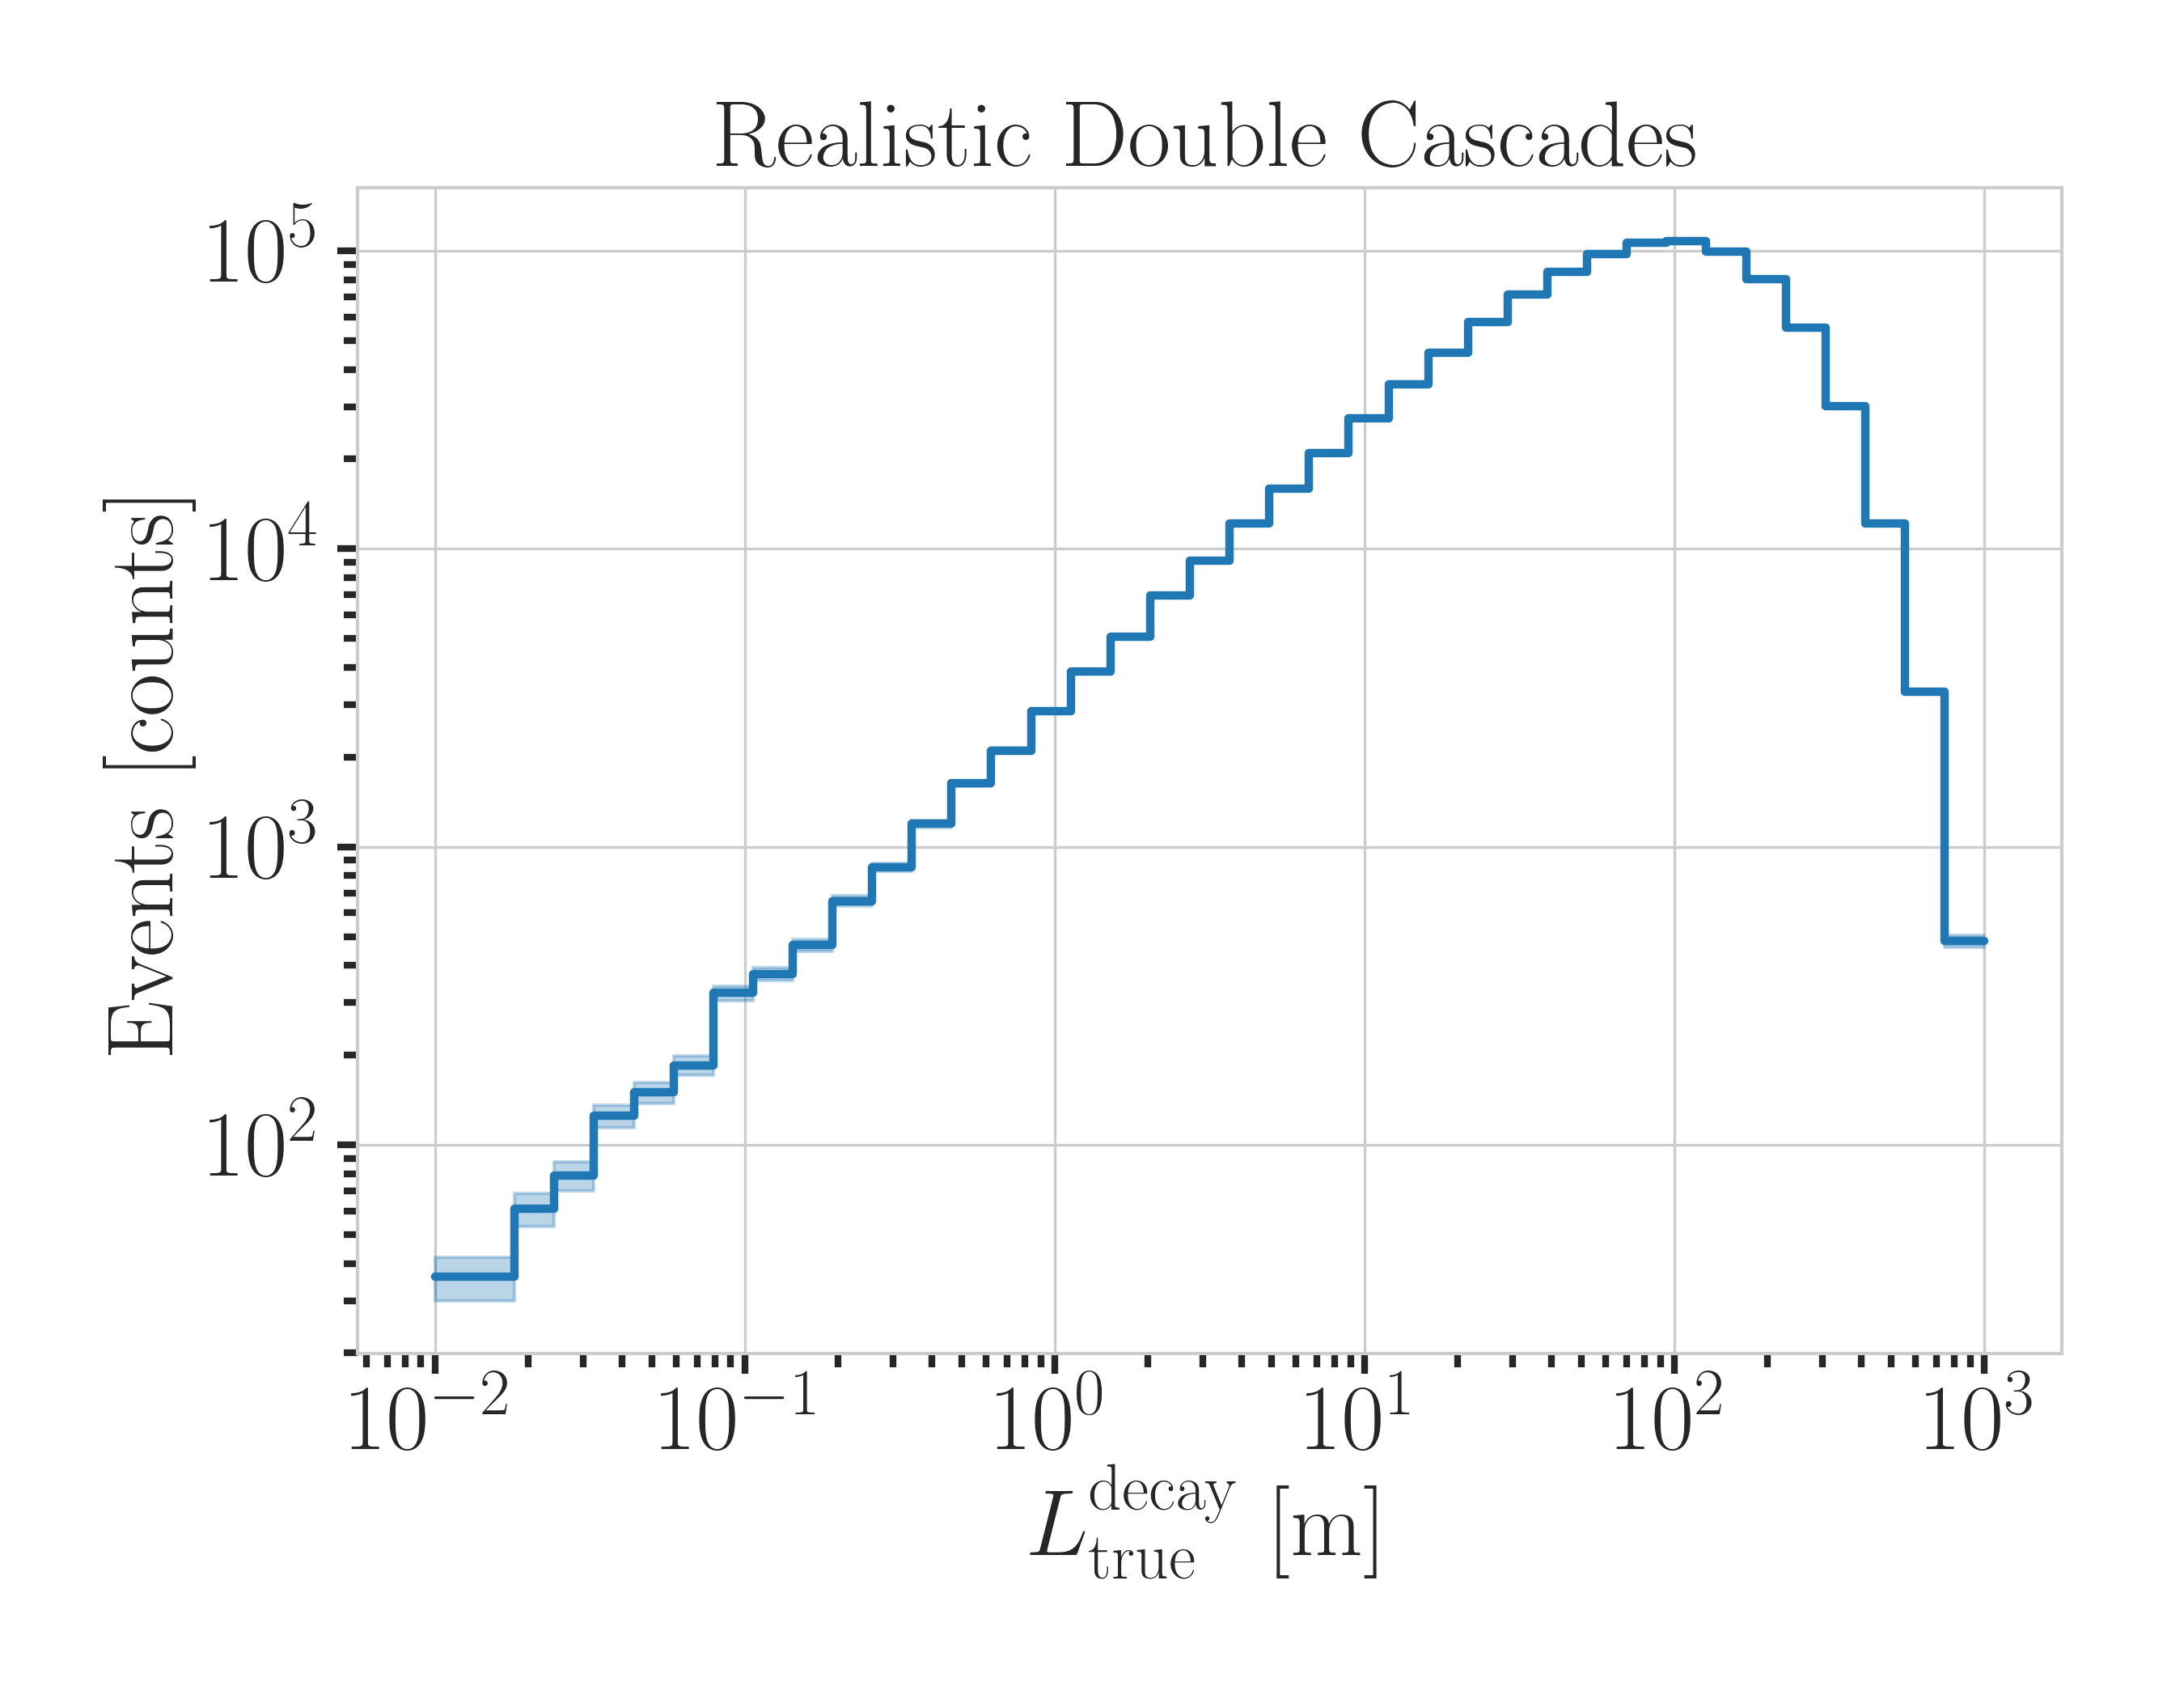
\includegraphics[width=.49\linewidth]{figures/model_independent_simulation/gen_level/194603_gen_level_1_d_distr_true_decay_length.png}
    \caption[Realistic model-independent simulation generation level distributions]{Generation level distributions of the realistic sample. Shown are the individual cascade energies and total energy (left) and decay lengths (right). It can be seen how the cascade energies can get very small, and the decay length follows a more realistic distribution spanning across several orders of magnitude.}
    \labfig{realistic_gen_distris}
\end{figure*}

To efficiently generate events in a way that produces distributions similar to what would be observed with DeepCore, one of the cascade positions is sampled inside the DeepCore volume by choosing its coordinates uniformly on a cylinder that is centered in DeepCore. This is similar to a trigger condition of one cascade always being inside the DeepCore fiducial volume. Choosing the direction of the event by sampling zenith and azimuth uniformly between \SIrange[range-phrase={~and~}]{70}{180}{\degree} and \SIrange[range-phrase={~and~}]{0}{360}{\degree}, respectively, the position of the other cascade can be inferred for a given decay length. This is done by assuming a travel speed of $c$, and choosing whether the cascade position that was sampled is the first cascade or the second cascade with a \SI{50}{\percent} chance. The zenith angle is chosen between straight up-going (zenith of \SI{180}{\degree}) and slightly down-going from above the horizon (\SI{70}{\degree}) to mimic an event selection that reduces atmospheric muons by rejecting events coming from above the horizon, but still incorporates some down-going events. All distributions are shown in \reffig{realistic_gen_distris_appendix}, and the sampling distributions/values are listed in \reftab{hnl_realistic_sample_sampling_distributions}.

\begin{table}[h]
    \small
        \begin{tabular}{ llll }
        \hline\hline
        \textbf{Variable} & \textbf{Distribution} & \textbf{Range/Value} \\
        \hline\hline
        energy (total) & power law $E^{-2}$ & \SIrange{1}{1000}{\gev} \\
        decay length & exponential e$^{-0.01L}$ & \SIrange{0}{1000}{\metre} \\
        zenith & uniform & \SIrange{70}{180}{\degree} \\
        azimuth & uniform & \SIrange{0}{360}{\degree} \\
        $x,y$ (one cascade) & uniform (circle) & $c$=(46.29, -34.88)\,\si{\metre}, $r$=\SI{150}{\metre} \\
        $z$ (one cascade) & uniform & \SIrange{-480.0}{-180.0}{\metre}\\
        \hline
        \end{tabular}
        \caption[Realistic model-independent simulation sampling distributions]{Generation level sampling distributions and ranges/values of the realistic model-independent simulation.}
    \labtab{hnl_realistic_sample_sampling_distributions}
\end{table}


\section{Model-Dependent Heavy Neutral Lepton Event Generation} \labsec{model_specific_simulation}

To estimate the HNL event expectation in IceCube DeepCore, depending on the specific model parameters, a generator was developed that is based on the HNL theory introduced in \refsec{hnl_theory}. For this work, only the interaction with the $\tau$-sector was taken into account ($|U_{\alpha4}^2|=0$, $\alpha=e,\mu$), which reduces the physics parameters of interest and relevant for the generation to the fourth heavy lepton mass, $m_4$, and the mixing, $|U_{\tau4}^2|$.

Due to the very low interaction rate of neutrinos, which are the source of HNL production, the event generation is performed in a way that forces every event to interact in a chosen sampling volume. The weight of each event is then calculated as the inverse of the simulated neutrino fluence
\begin{equation}
    w_\rm{gen} = \frac{1}{F_{\mathrm{sim}}} \frac{1}{N_{\mathrm{sim}}}
    \;,
    \labeq{neutrino_generation_weight}
\end{equation}
where $F_{\rm{sim}}$ is the number of neutrino events per energy, time, area, and solid angle, and $N_{\rm{sim}}$ is the number of simulated events. If this weight is multiplied by the livetime and the theoretically expected neutrino flux for a given physical model, it results in the number of expected events in the detector for this particular MC event.

The generator uses a customized \textit{\textsc{LeptonInjector} (LI)} version to create the events and \textit{\textsc{LeptonWeighter} (LW)} to weight them~\sidecite{IceCube:2020tcq}. The modified LI and the essential components needed for the HNL simulation are described in the next sections, followed by the description of the weighting scheme and the sampling distributions chosen for the generation.


\subsection{Custom LeptonInjector} \labsec{custom_leptoninjector}

In its standard version, the LI generator produces neutrino interactions by injecting a lepton and a hadronic cascade at the interaction vertex of the neutrino, where the lepton is the charged (neutral) particle produced in a CC (NC) interaction and the cascade is the hadronic cascade from the nucleus that is breaking apart. The hadronic cascade is stored as a specific object of type \textit{Hadrons}, which triggers the correct simulation of the shower development in the following simulation steps. Below \SI{30}{\gev} the individual hadrons are simulated using \textsc{Geant4}~\sidecite{geant4} while for higher energies an analytical approximation from~\cite{raedel_wiebusch_cherenkov_yield} is used. The main differences to an EM cascade is that part of the energy will not be observed, because it goes into neutral particles, and that the spatial development of the shower is different as discussed in \refsec{hadronic_showers}. Both objects are injected with the same $(x,y,z,t)$ coordinates and the kinematics are sampled from the differential and total cross-sections that are one of the inputs to LI.

\begin{figure}[h]
    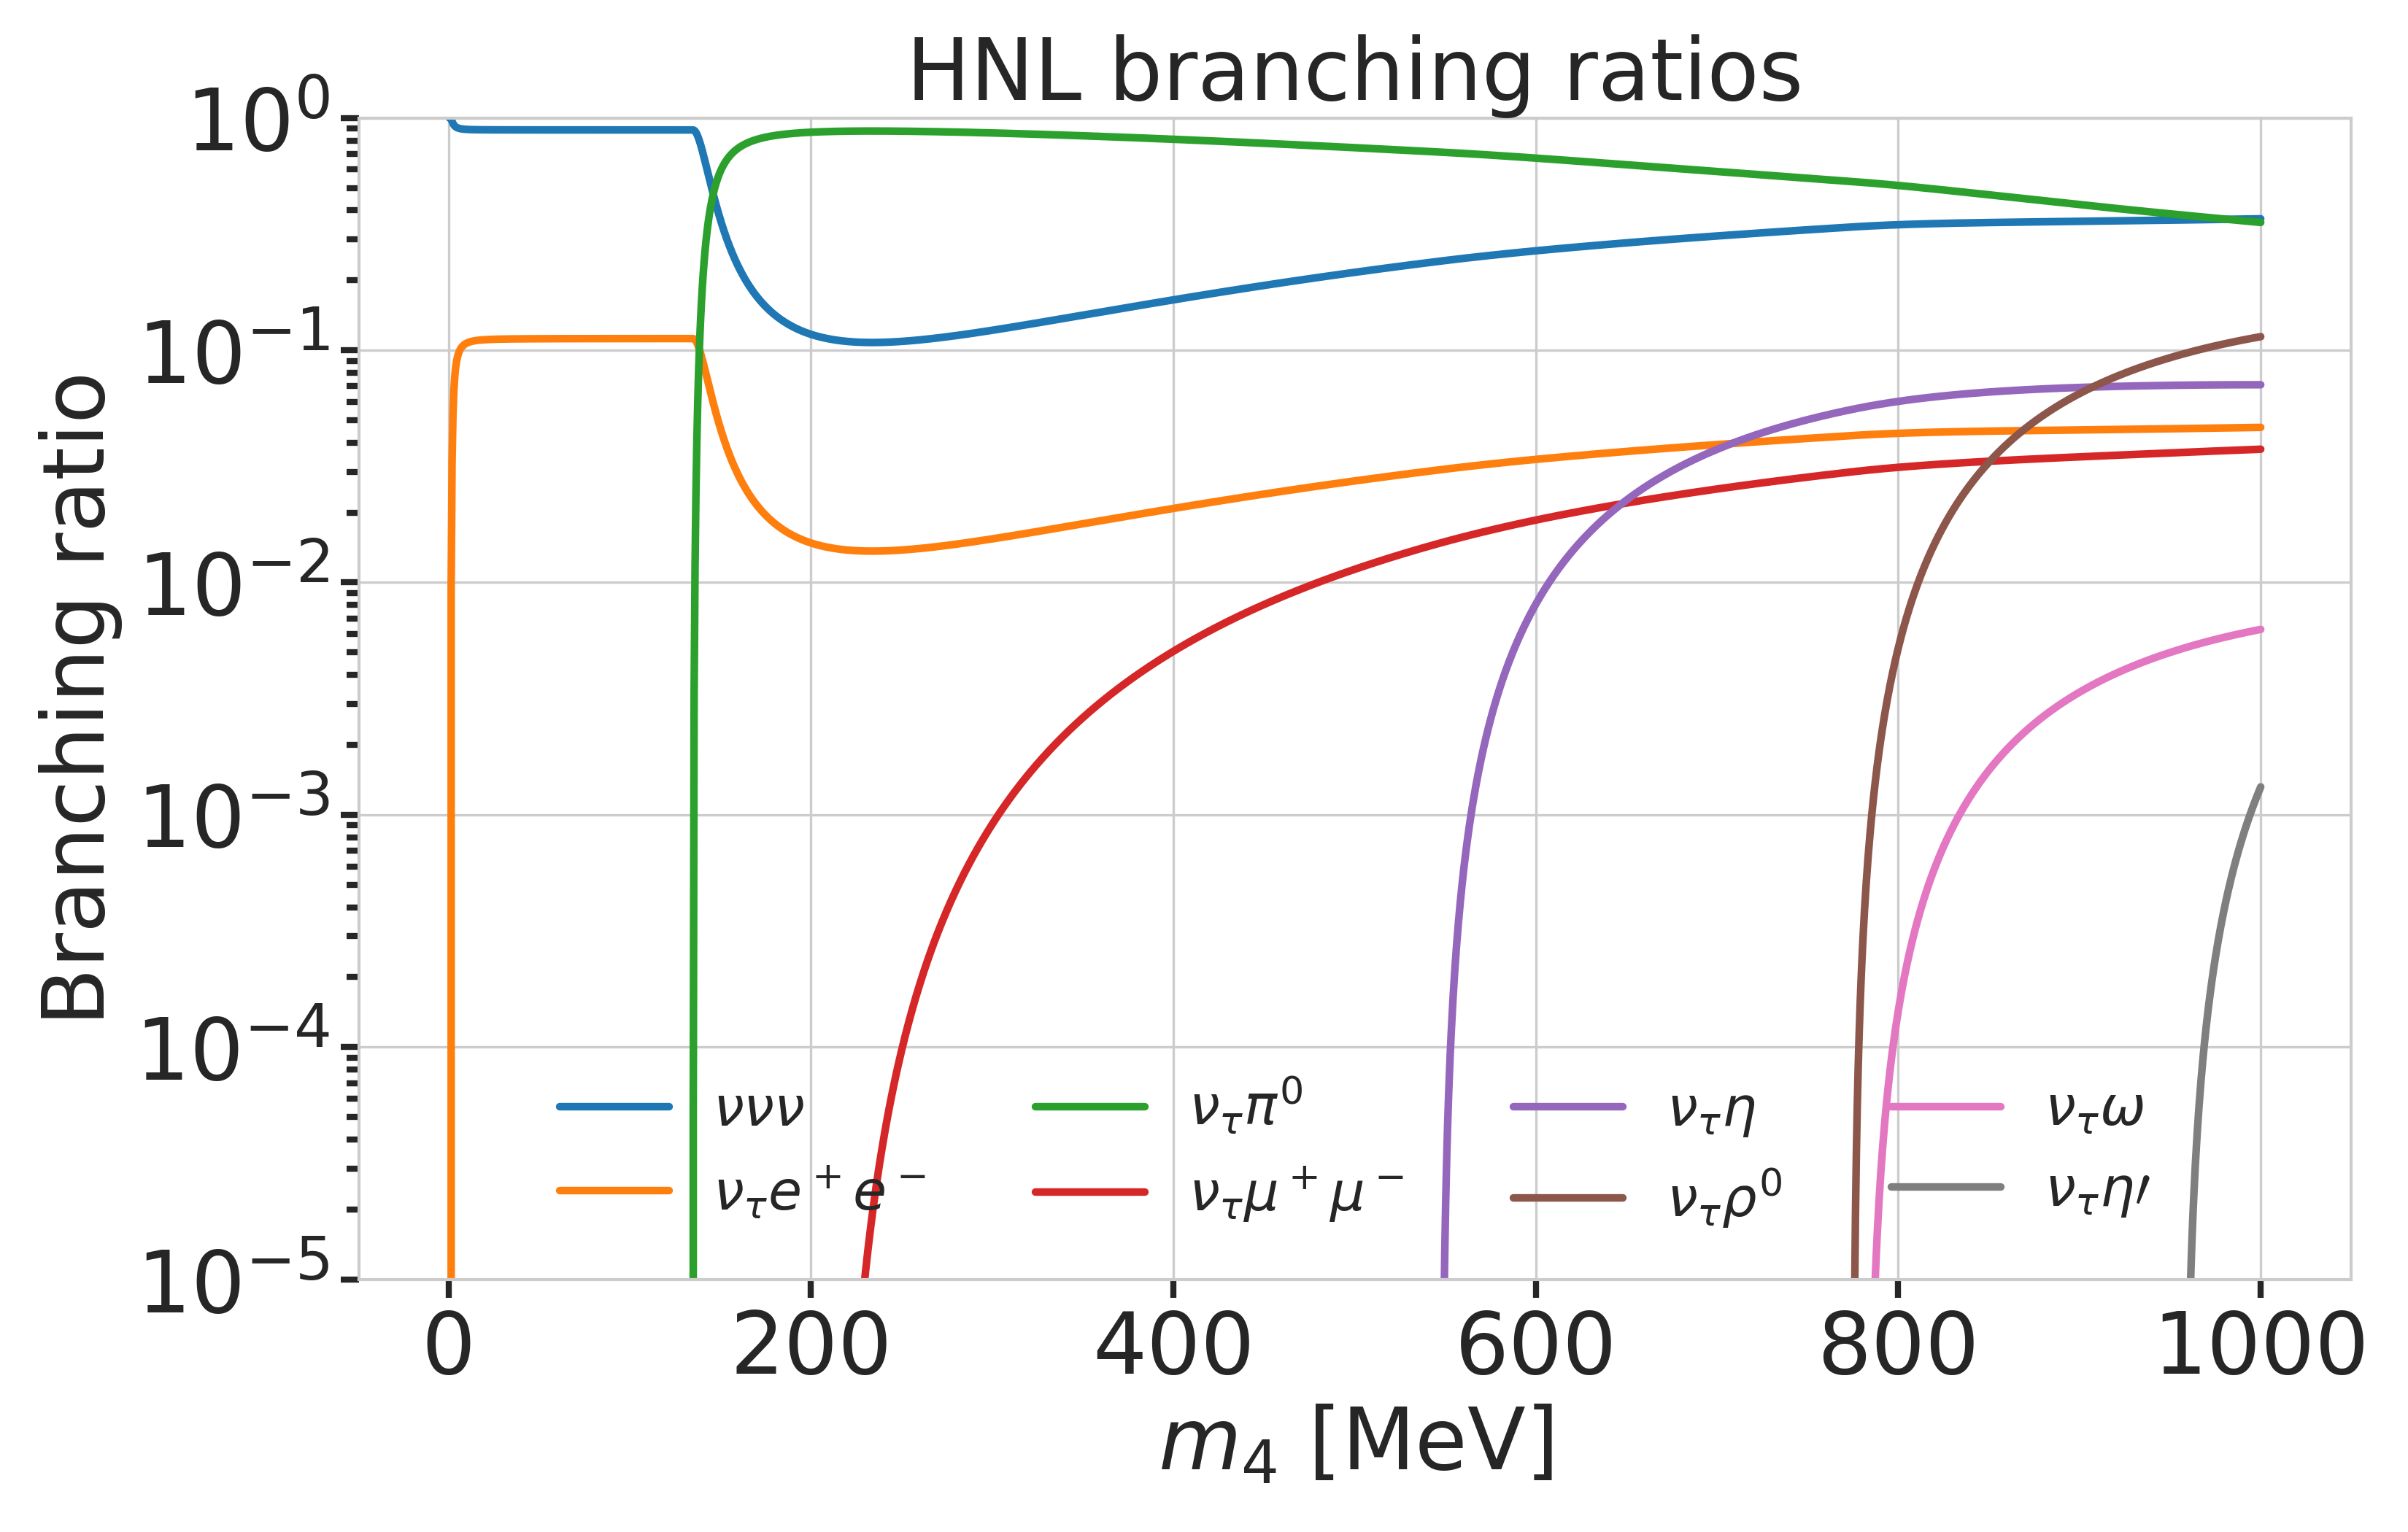
\includegraphics{hnl_simulation/decay_theory/branching_ratios_linear_up_to_1.0_GeV.png}
    \caption[HNL branching ratios]{Branching ratios of the HNL within the mass range considered in this work, only considering $|U_{\tau4}^2| \neq 0$, calculated based on the results from~\cite{Coloma:2020lgy}.}
    \labfig{hnl_branching_ratios}
\end{figure}

In the modified version, the SM lepton at the interaction vertex is replaced by the new HNL particle, where the interaction cross-sections are replaced by custom, mass dependentg HNL cross-sections. The HNL is forced to decay after a chosen distance\sidenote{The explicit sampling distributions and ranges can be found in \refsec{hnl_sampling_distributions}.} to produce secondary SM particles, where the decay mode is chosen with a probability given by the mass dependent branching ratios from the kinematically accessible decay modes shown in \reffig{hnl_branching_ratios}. The cross-section and decay width calculations were implemented for this purpose and will be explained in more detail in the following. Another addition to LI is that the decay products of the HNL are also stored. These HNL daughter particles form the second cascade, not as a single hadronic cascade object, but as the explicit particles forming the shower. They are injected with the correctly displaced position and delayed time from the interaction vertex, given the HNL decay length. The kinematics of the two-body decays are computed analytically, while the 3-body decay kinematics are calculated with \textsc{MadGraph4} (v3.4.0)~\cite{madgraph4}, which will also be explained further below. Independent of the number of particles in the final state of the HNL decay, the kinematics are calculated/simulated at rest and then boosted along the HNL momentum.

Muons produced in those decays are propagated using \textsc{Proposal}~\sidecite{proposal}, also simulating their Cherenkov light output. The shower development of gamma rays, electrons, and positrons below \SI{100}{\mega\electronvolt} is simulated using Geant4 and for higher energies the analytical approximation is used again~\cite{raedel_wiebusch_cherenkov_yield}.

The injection is done using the LI \textit{volume mode}, for the uniform injection of the primary particle on a cylindrical volume, adding \SI{50}{\percent} of the events with $\nu_\tau$ and the other half with $\bar{\nu}_\tau$ as primary particle types. The generator takes the custom double-differential/total cross-section splines described below and the parameters defining the sampling distributions as inputs.


\subsubsection{Cross-Sections}

The cross-sections are calculated using the \textsc{NuXSSplMkr}~\cite{xsecmaker} software, which is a tool to calculate neutrino cross-sections from \textit{parton distribution functions (PDFs)} and then fit to an N-dimensional tensor-product B-spline surface~\sidecite{photospline} to produce the splines that can be read and used with LI/LW. The tool was modified to produce the custom HNL cross-sections, where the main modification to calculate the cross-sections for the $\nu_\tau$-NC interaction into the new heavy mass state is the addition of a kinematic condition to ensure that there is sufficient energy to produce the heavy mass state. It is the same condition fulfilled for the CC case, where the outgoing charged lepton mass is non-zero. Following~\sidecite{Levy:2004rk} (equation 7), the condition
\begin{equation}
    (1 + x \delta_N) h^2 - (x + \delta_{4}) h + x \delta_{4} \leq 0
    \;
    \labeq{hnl_kinematic_condition}
\end{equation}
is implemented for the NC case in the NuXSSplMkr code. Here
\begin{align}
    \delta_{4} ={}& \frac{m_4^2}{s-M^2}
    \;, \\
    \delta_{N} ={}& \frac{M^2}{s-M^2}
    \;, \rm{and} \\
    h \overset{\textit{def}}{=}& xy + \delta_{4}
    \;,
    \labeq{hnl_kinematic_condition_variables}
\end{align}
with $x$ and $y$ being the Bjorken variables, $m_4$ and $M$ the mass of the heavy state and the target nucleon, respectively, and $s$ the center of mass energy squared. The custom version was made part of the open source NuXSSplMkr software and can thus be found in~\cite{xsecmaker}. The result of this kinematic condition is that events cannot be produced for combinations of energy, $x$, $y$ that do not have sufficient energy to produce the outgoing, massive lepton. This results in a reduction of the cross-section towards lower energies, which scales with the assumed mass of the HNL. This effect can be seen in \reffig{custom_hnl_cross_sections}.

\begin{figure*}[h]
    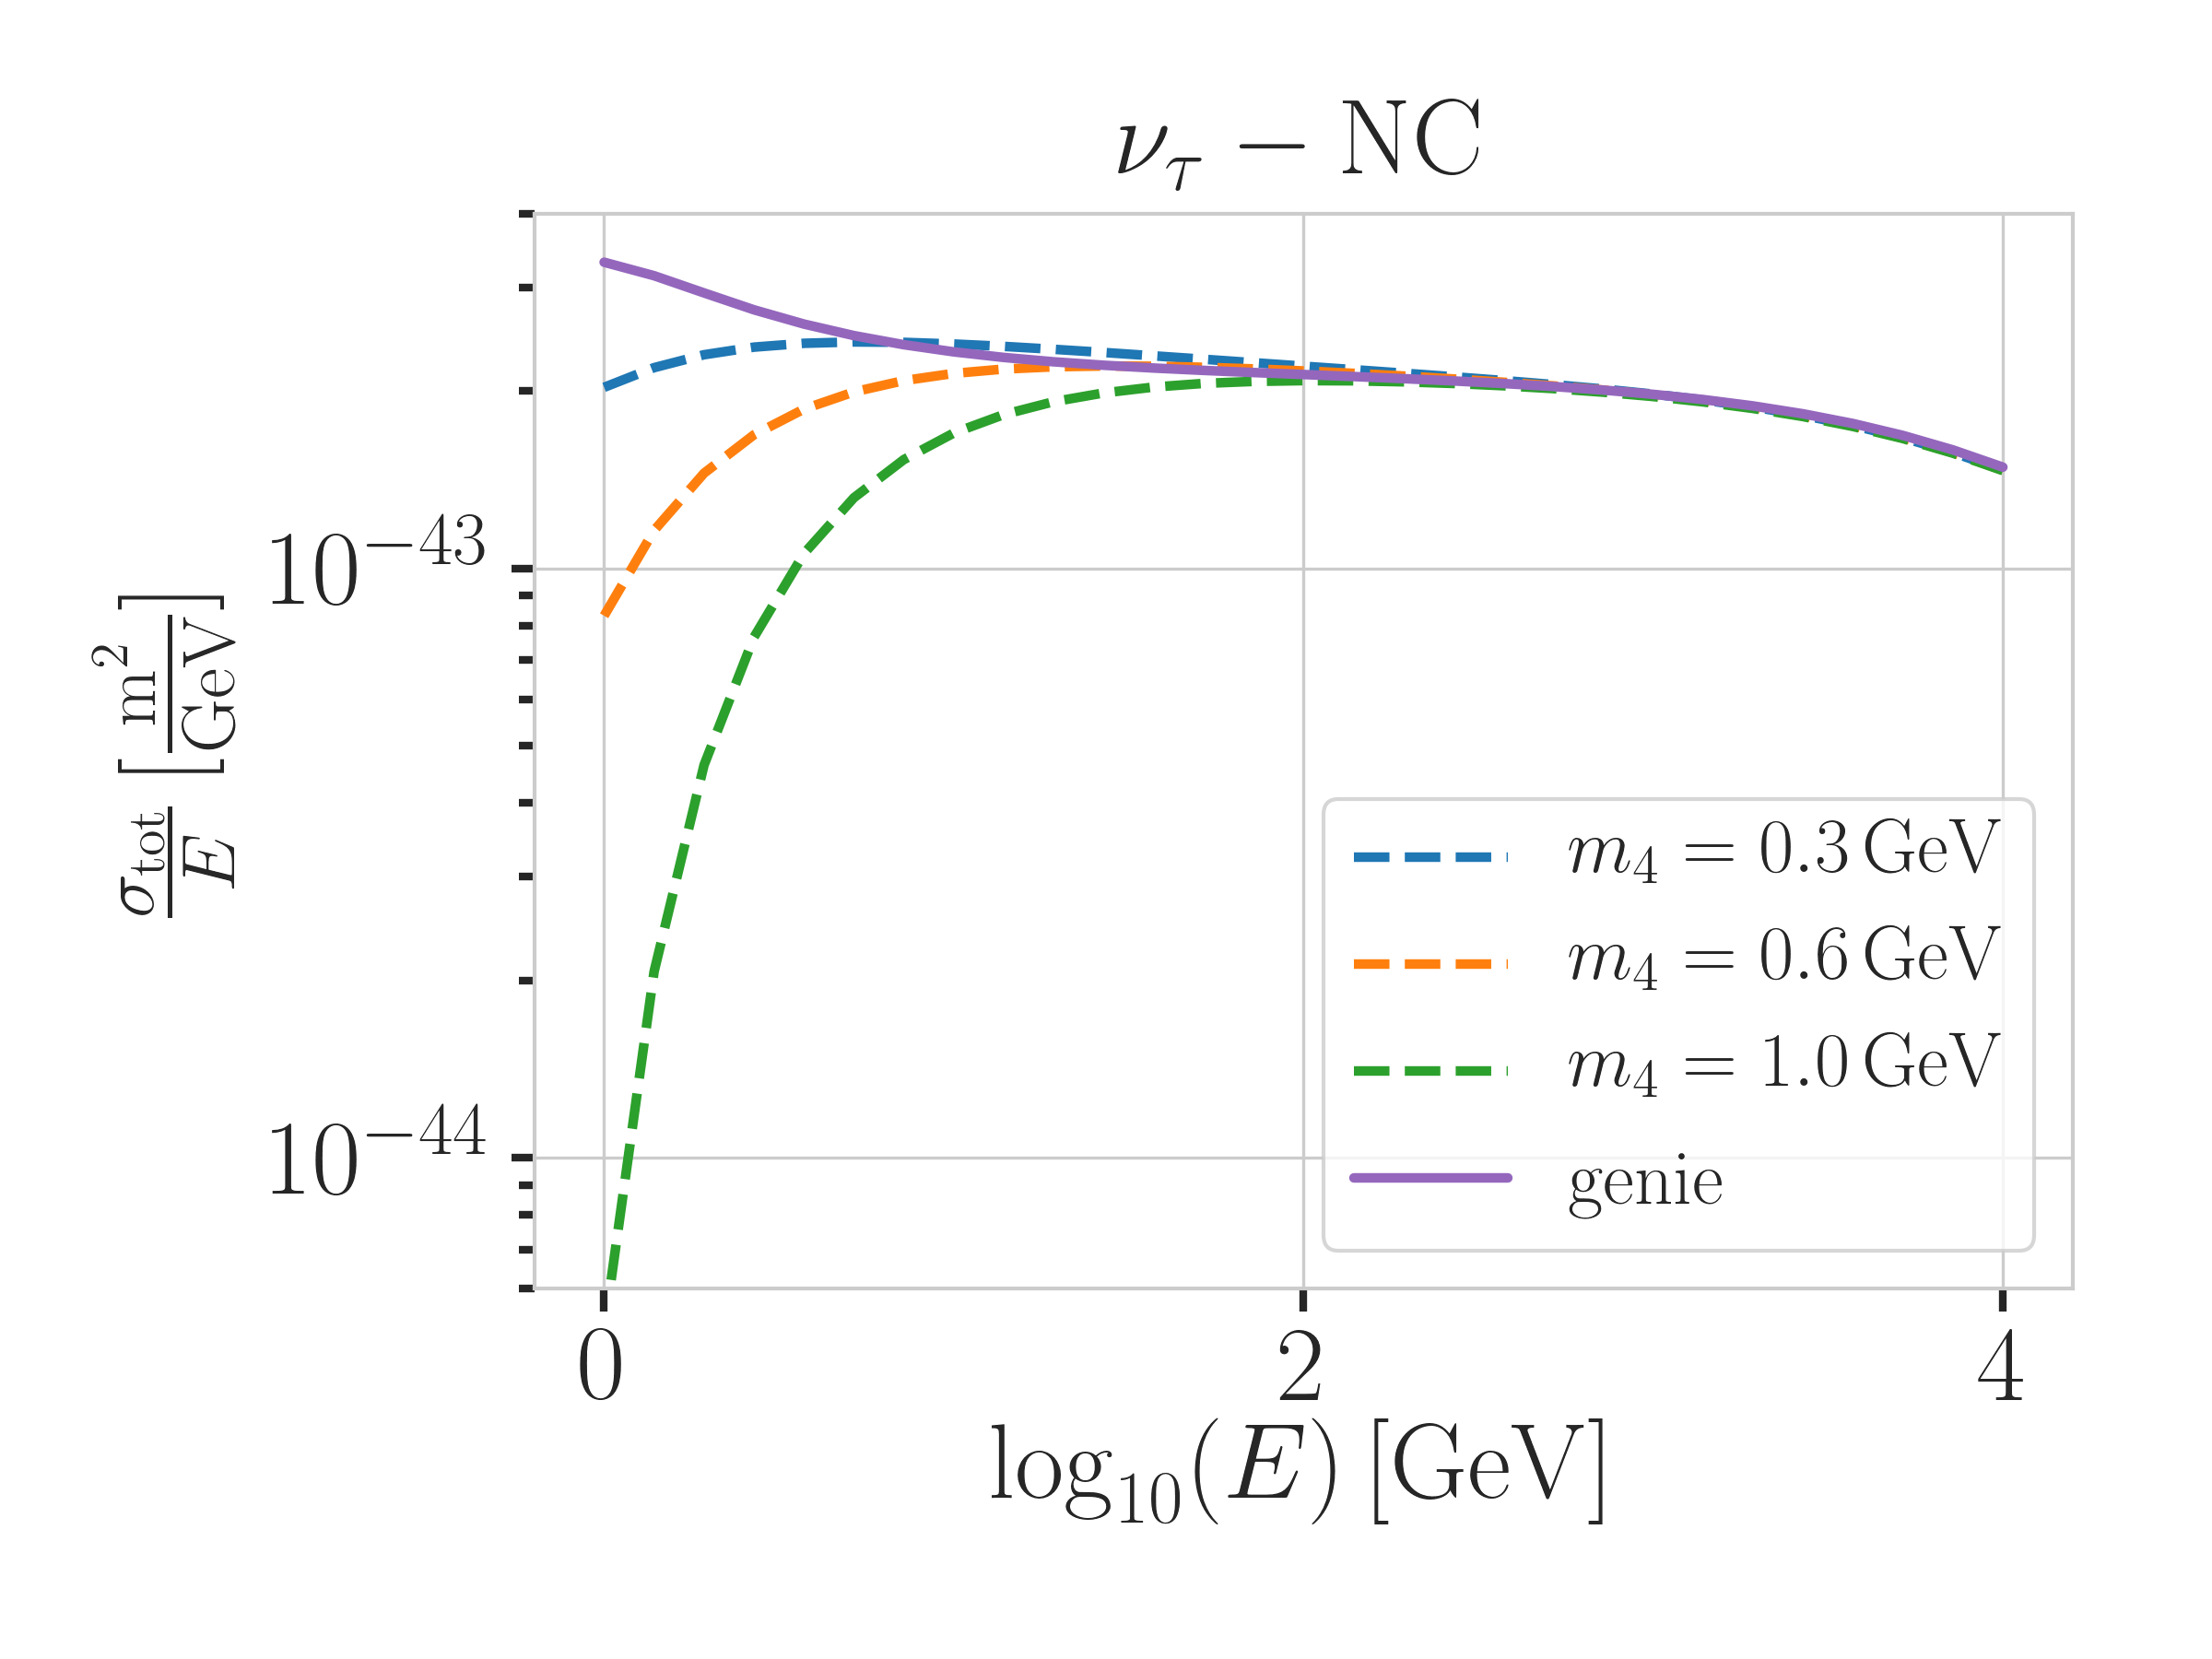
\includegraphics[width=.49\linewidth]{figures/hnl_simulation/cross_sections/custom_HNL_thesis_sigma-nutau-N-nc.png}
    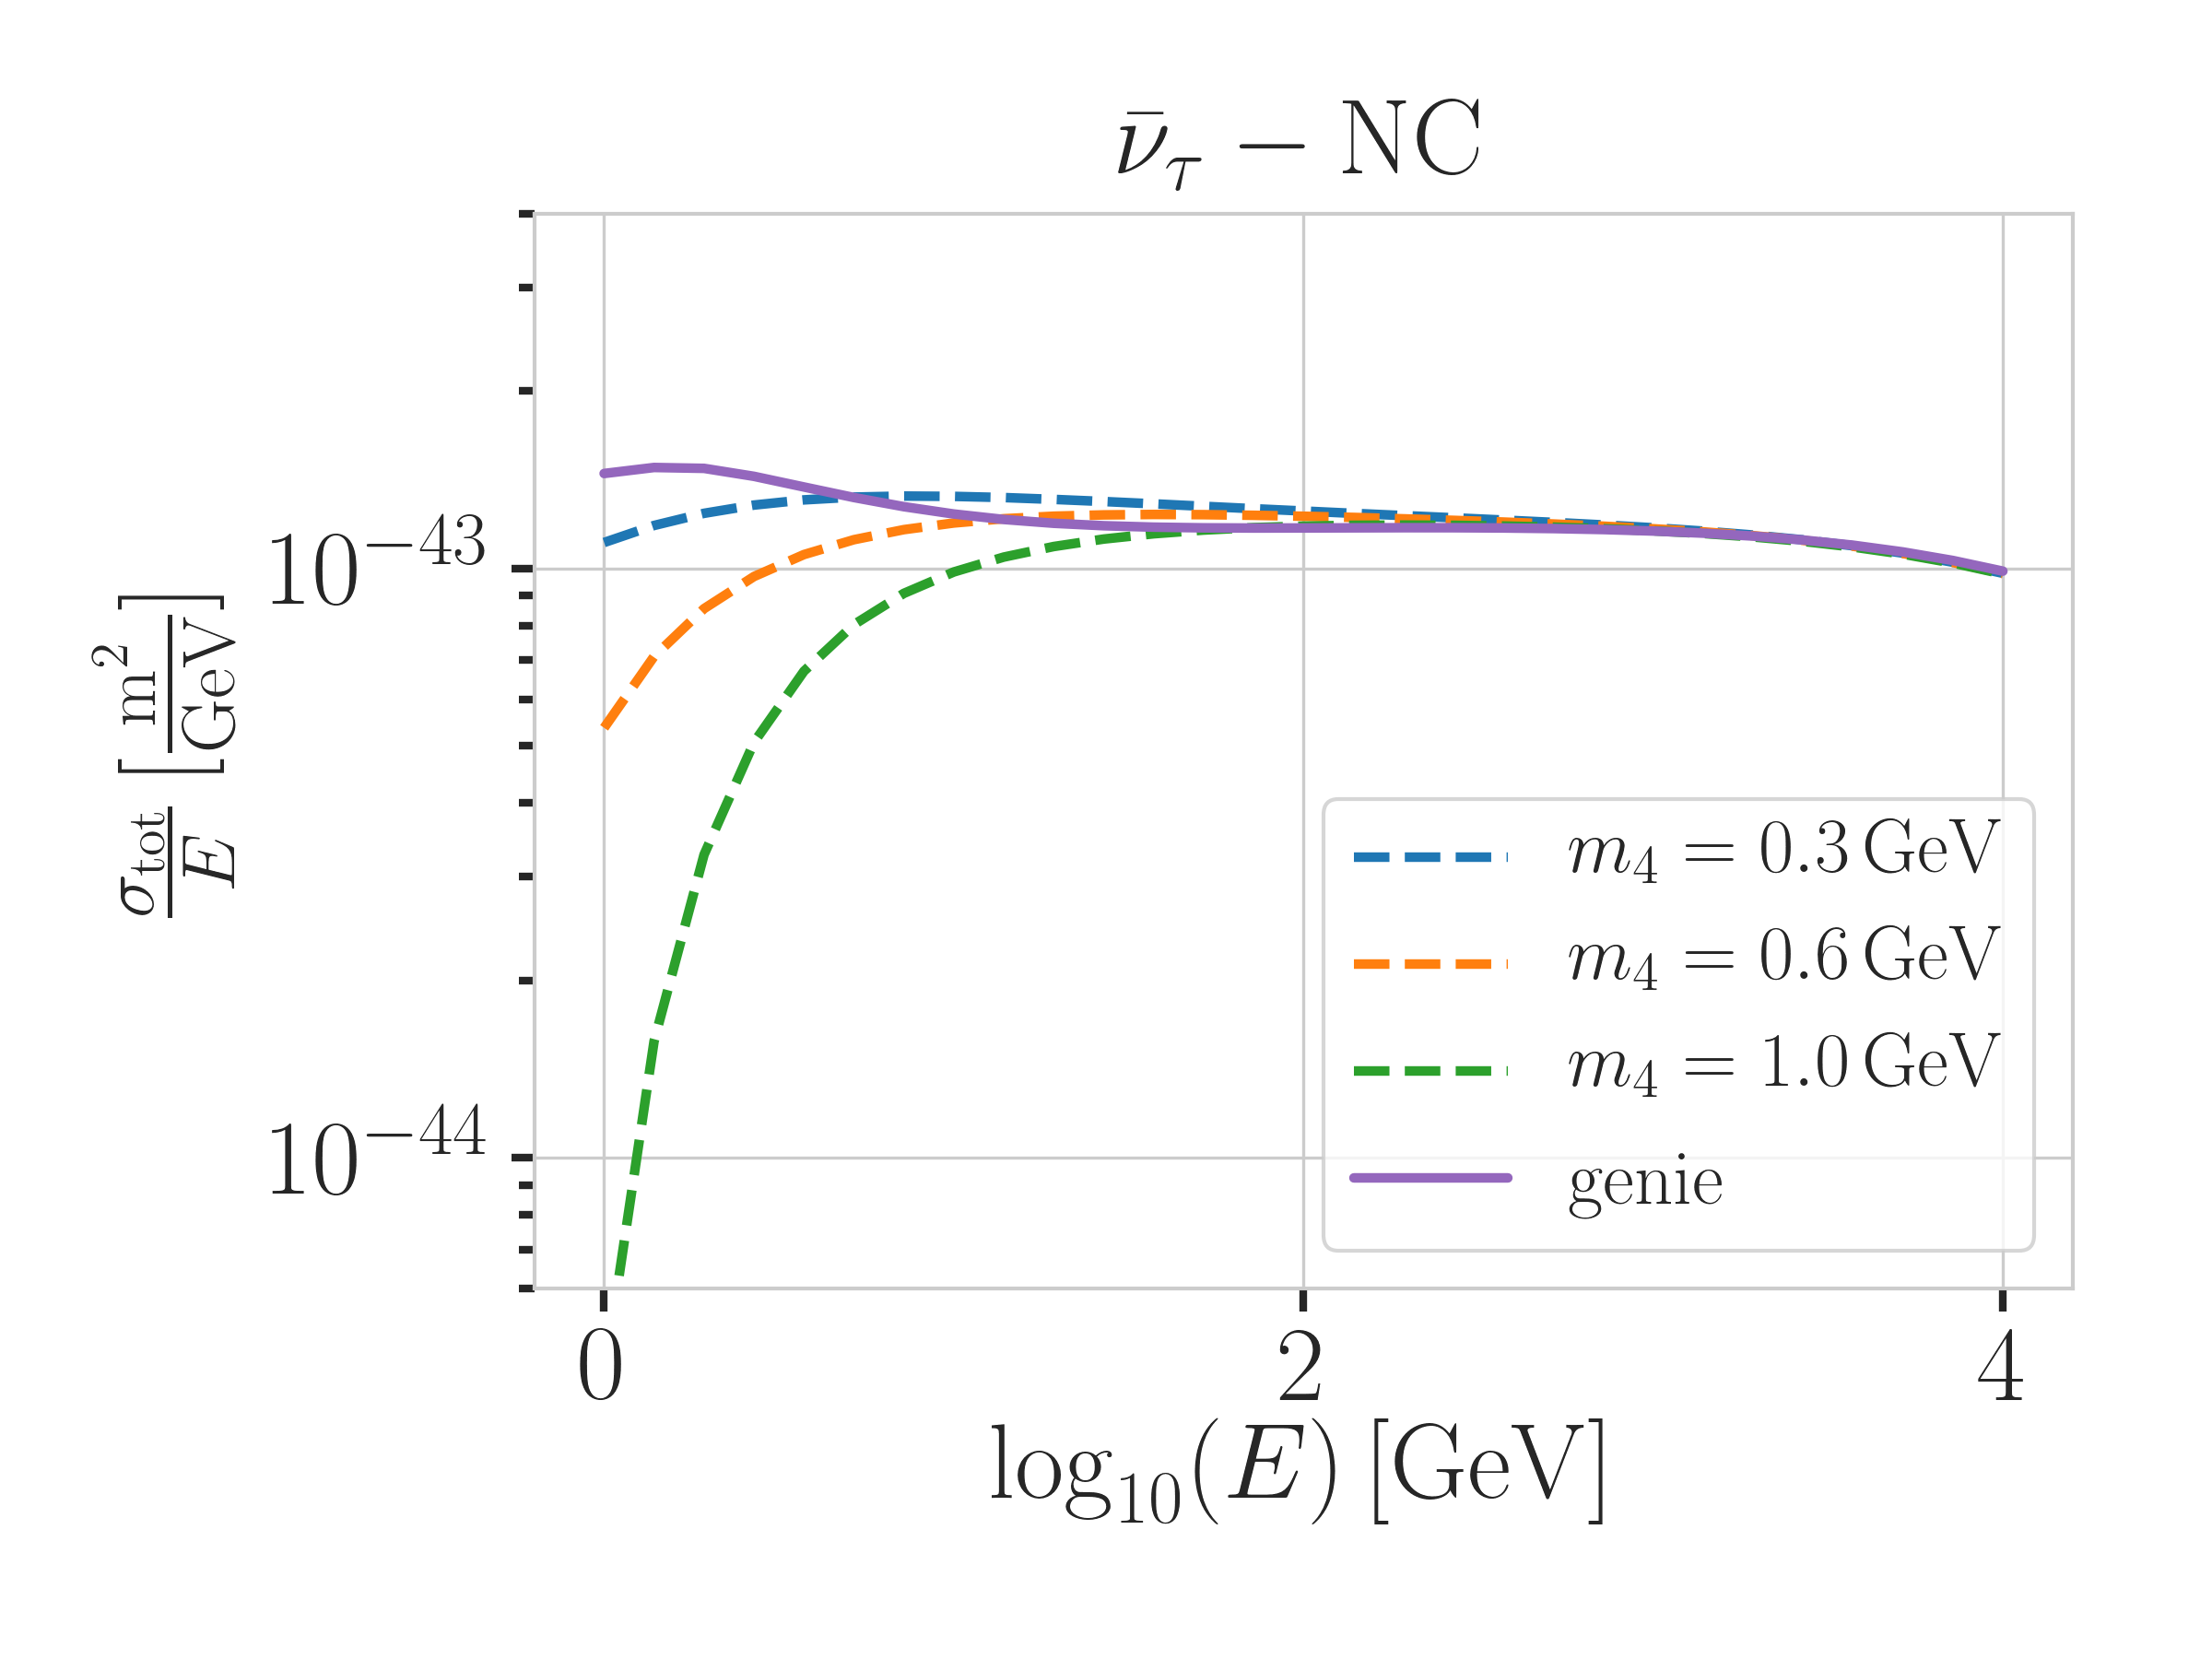
\includegraphics[width=.49\linewidth]{figures/hnl_simulation/cross_sections/custom_HNL_thesis_sigma-nutaubar-N-nc.png}
    \caption
    [Custom HNL total cross-sections]{Custom HNL total cross-sections for the three target masses compared to the total ($\nu_\tau$/$\bar{\nu}_\tau$ NC) cross-sections used for SM neutrino simulation production with GENIE.}
    \labfig{custom_hnl_cross_sections}
\end{figure*}

The GRV98LO~\sidecite{grv98_pdf} PDFs were added to the cross-section spline maker and used to create the HNL cross-sections for consistency with the neutrino simulation. The double-differential ($\rm{d}^2\sigma/\rm{d}x\rm{d}y$) and total ($\sigma$) cross-sections were produced for the chosen target HNL masses and then splined in energy, $x$, and $y$ for $\rm{d}^2\sigma/\rm{d}x\rm{d}y$, and in energy for $\sigma$. \reffig{custom_hnl_cross_sections} shows the total cross-sections that were produced compared to the cross-section used for the production of the SM $\nu_\tau/\bar{\nu}_\tau$ NC background simulation. They agree above $\sim\SI{200}{\GeV}$, where the modification should not have any effect on the cross-sections. This is the desired result of using the identical input PDFs, and confirms that the unmodified cross-sections produced with NuXSSplMkr agree with the GENIE cross-sections.


\subsubsection{Decay Channels}

The accessible decay channels are dependent on the mass of the HNL and the allowed mixing. For this analysis, where only $|U_{\tau4}|^2 \neq 0$, the decay channels considered are listed in \reftab{hnl_decay_channels} and the corresponding branching ratios are shown in \reffig{hnl_branching_ratios}. The individual branching ratio for a specific mass is calculated as $\mathrm{BR}_i(m_4)=\Gamma_i(m_4)/\Gamma_\mathrm{total}(m_4)$, where $\Gamma_\mathrm{total}(m_4)=\sum\Gamma_i(m_4)$. They can be seen in \reffig{hnl_decay_modes_log_decay_width}, where the individual decay widths $\Gamma_i$ are shown, which are computed using an implementation of the state-of-the-art calculations from~\cite{Coloma:2020lgy}. The formulae for these calculations are explicitly listed in the following.

\begin{margintable}[-1cm]
    \begin{tabular} { lr }
        \hline\hline 
        \textbf{Channel} & \textbf{Opens}  \\
        \hline\hline 
        $\nu_4 \rightarrow \nu_\tau \nu_\alpha \bar{\nu_\alpha}$ & \SI{0}{\MeV} \\
        $\nu_4 \rightarrow \nu_\tau e^+ e^-$ & \SI{1}{\MeV} \\
        $\nu_4 \rightarrow \nu_\tau \pi^0$ & \SI{135}{\MeV} \\
        $\nu_4 \rightarrow \nu_\tau \mu^+ \mu^-$ & \SI{211}{\MeV} \\
        $\nu_4 \rightarrow \nu_\tau \eta$ & \SI{548}{\MeV} \\
        $\nu_4 \rightarrow \nu_\tau \rho^0$ & \SI{770}{\MeV} \\
        $\nu_4 \rightarrow \nu_\tau \omega$ & \SI{783}{\MeV} \\
        $\nu_4 \rightarrow \nu_\tau \eta'$ & \SI{958}{\MeV} \\
        \hline
    \end{tabular}
    \caption[HNL mass dependent decay channels]{Possible decay channels of the HNL, considering only $|U_{\tau4}|^2 \neq 0$, and the mass at which each channel opens.}
    \labtab{hnl_decay_channels}
\end{margintable}

\begin{figure}[h]
    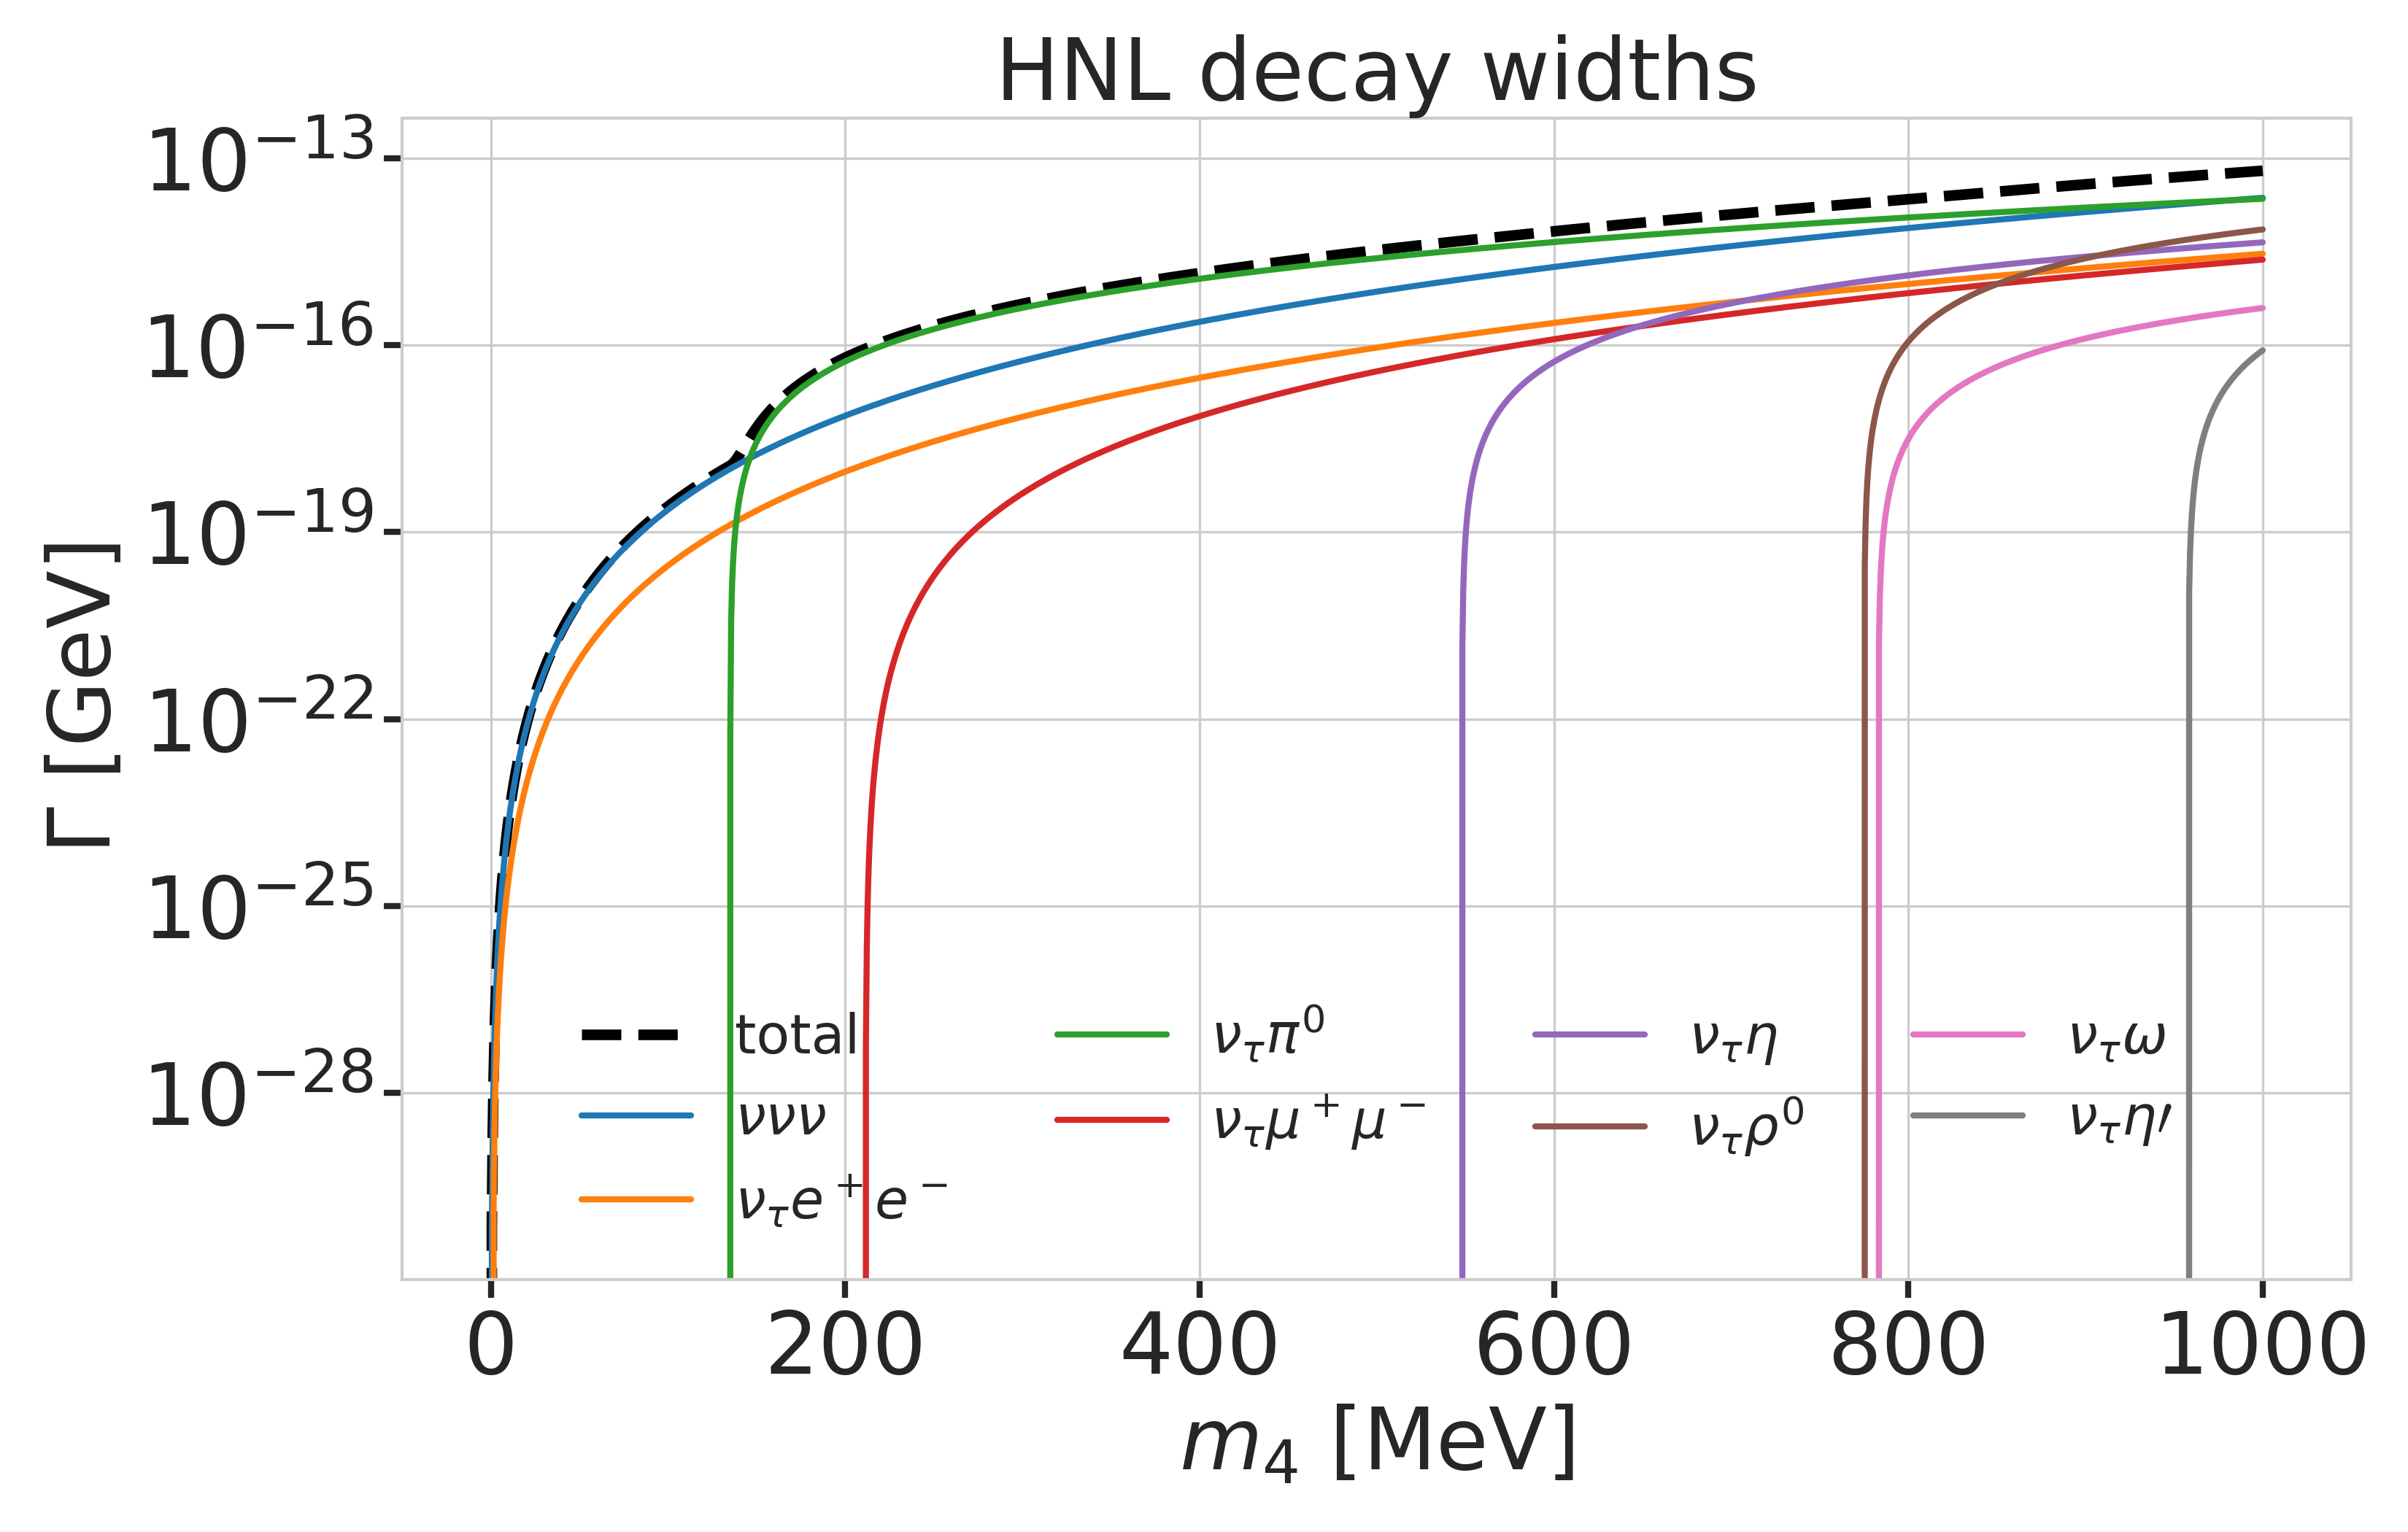
\includegraphics{figures/hnl_simulation/decay_theory/hnl_decay_widths_up_to_1.0_GeV_linear.png}
    \caption[HNL decay widths]{Decay widths of the HNL within the mass range considered, calculated based on the results from~\cite{Coloma:2020lgy}. Given the existing constraints on $|U_{e4}|^{2}$ and $|U_{\mu4}|^{2}$, we consider that the corresponding decay modes are negligible.}
    \labfig{hnl_decay_modes_log_decay_width}
\end{figure}


\paragraph{2-Body Decay Widths:} The decay to a neutral pseudoscalar meson is
\begin{equation}
    \Gamma_{\nu_4 \rightarrow \nu_\tau P} = |U_{\tau4}|^2 \frac{G_F^2 m_4^3}{32\pi} f_P^2 (1-x_p^2)^2
    \;,
    \labeq{gamma_nu_P}
\end{equation}
with $x_P = m_P/m_4$ and the \textit{effective decay constants $f_P$} given by
\begin{align}
    f_{\pi^0} ={}& +\SI{0.1300}{\GeV}\;, \\
    f_{\eta} ={}& +\SI{0.0816}{\GeV}\;, \rm{and} \\
    f_{\eta'} ={}& -\SI{0.0946}{\GeV}\;,
    \labeq{gamma_nu_P_f_factors}
\end{align}
while the decay to a neutral vector meson is given by
\begin{equation}
    \Gamma_{\nu_4 \rightarrow \nu_\tau V} = |U_{\tau4}|^2 \frac{G_F^2 m_4^3}{32\pi} \bigg(\frac{f_V}{m_V}\bigg)^2 g_V^2 (1+2x_V^2) (1-x_V^2)^2
    \;,
    \labeq{gamma_nu_V}
\end{equation}
with $x_V = m_V/m_4$,
\begin{align}
    f_{\rho^0} ={}& \SI{0.171}{\square\GeV}\;, \\
    f_{\omega} ={}& \SI{0.155}{\square\GeV}\;,
    \labeq{gamma_nu_V_f_factors}
\end{align}
and
\begin{align}
    g_{\rho^0} ={}& 1-2\sin^2{\theta_w}\;, \\
    g_{\omega} ={}& \frac{-2\sin^2{\theta_w}}{3}\;,
    \labeq{gamma_nu_V_g_factors}
\end{align}
and $\sin^2{\theta_w}=0.2229$~\sidecite{codata2018}, where $\theta_w$ is the Weinberg angle.


\paragraph{3-Body Decay Widths:} The (invisible) decay to three neutrinos, one of flavor $\tau$ and two of any flavor $\alpha$, is
\begin{equation}
    \Gamma_{\nu_4 \rightarrow \nu_\tau \nu_\alpha \bar{\nu_\alpha}} = |U_{\tau4}|^2 \frac{G_F^2 m_4^5}{192\pi^3}
    \;,
    \labeq{gamma_nu_nu_nu}
\end{equation}
while the decay to two charged leptons (using $x_\alpha = (m_\alpha/m_4)^2)$ of the same flavor reads
\begin{equation}
    \Gamma_{\nu_4 \rightarrow \nu_\tau l_\alpha^+ l_\alpha^-} = |U_{\tau4}|^2 \frac{G_F^2 m_4^5}{192\pi^3} \big[ C_1 f_1(x_\alpha) + C_2 f_2(x_\alpha) \big]
    \;,
    \labeq{gamma_nu_ll_full}
\end{equation}
with the constants defined as
\begin{align}
    C_1 ={}& \frac{1}{4}(1-4\sin^2{\theta_w}+8\sin^4{\theta_w})\;, \\
    C_2 ={}& \frac{1}{2}(-\sin^2{\theta_w}+2\sin^4{\theta_w})\;,
    \labeq{gamma_nu_ll_c1_c2}
\end{align} 
the functions as
\begin{align}
    f_1(x_\alpha) = (1-14x_\alpha-2x_\alpha^2-12x_\alpha^3)\sqrt{1-4x_\alpha}+12x_\alpha^2(x_\alpha^2-1)L(x_\alpha) \;, \\
    f_2(x_\alpha) = 4[x_\alpha(2+10x_\alpha-12x_\alpha^2)\sqrt{1-4x_\alpha}+6x_\alpha^2(1-2x_\alpha+2x_\alpha^2)L(x_\alpha)] \;,
    \labeq{gamma_nu_ll_f1_f2}
\end{align}
and
\begin{equation}
    L(x) = \ln \biggl( \frac{ 1-3x_\alpha-(1-x_\alpha)\sqrt{1-4x_\alpha} }{ x_\alpha(1+\sqrt{1-4x_\alpha}) } \biggr)
    \;.
    \labeq{gamma_nu_ll_l}
\end{equation}


\subsubsection{Analytical 2-Body Decay Kinematics}

Following the review of~\sidecite{PDG_review_2022}, the 4-vector defining the kinematics of a particle is $p=(E,\vec{p})$, with its energy, $E$, and 3-momentum, $\vec{p}$. Squaring it gives the mass, $p^2=E^2-\vec{p}^2=m^2$, while the velocity is $\vec{\beta}=\vec{p}/E$. If the HNL with mass $m_4$ decays into two particles with masses $m_1$ and $m_2$, their 3-momenta in the rest frame of the HNL are given by
\begin{equation}
    |\vec{p}_1| = |\vec{p}_2| = \frac{\lambda^{1/2}(m_4^2,m_1^2,m_2^2)}{2m_4}
    \;,
    \labeq{2body_momenta}
\end{equation}
where $\lambda(x,y,z)=x^2+y^2+z^2-2xy-2xz-2yz$. The energy of the particles is then given by
\begin{equation}
    E_1 = \frac{m_4^2+m_1^2-m_2^2}{2m_4}
    \;,
    \labeq{2body_energies}
\end{equation}
and equivalently for $E_2$. The 4-vectors of the particle are then boosted to the lab frame, where the HNL is moving with velocity $\vec{\beta}$.


\subsubsection{Simulated 3-Body Decay Kinematics}

The 3-body decay kinematics cannot be computed analytically, instead, we employ MadGraph4 for this purpose. MadGraph is a tool to simulate particle collisions and decay processes, and is widely used in the high-energy physics community. The 3-body decay kinematics are calculated in the rest frame of the HNL, using decay diagrams calculated with \textsc{FeynRules 2.0}~\sidecite{feynrules2} and the Lagrangians derived in~\sidecite{Coloma:2020lgy} as input. The \textit{Universal FeynRules Output (UFO)} from \textsc{effective\_HeavyN\_Majorana\_v103} were used for our calculation. For each mass and corresponding decay channels, we produce $10^6$ decay kinematic variations in the rest frame and store those. During event generation, we uniformly select one of those events to simulate the decay kinematics of a 3-body decay.


\subsection{Sampling Distributions} \labsec{hnl_sampling_distributions}

\begin{table}[H]
    \centering
    \begin{tabular} { lll }
        \hline \hline 
        \textbf{Variable} & \textbf{Distribution} & \textbf{Range/Value} \\
        \hline \hline 
        energy & $E^{-2}$ & [\SI{2}{\GeV}, \SI{1e4}{\GeV}] \\
        zenith & uniform (in $\cos(\theta)$) & [\SI{80}{\degree}, \SI{180}{\degree}] \\
        azimuth & uniform & [\SI{0}{\degree}, \SI{360}{\degree}] \\
        vertex $x,y$ & uniform (on circle) & $r$=\SI{600}{\metre} \\
        vertex $z$ & uniform & \SIrange{-600}{0}{\metre} \\
        $m_\mathrm{4}$ & fixed & [0.3, 0.6, 1.0]\,\si{\GeV} \\
        $L_\mathrm{decay}$ & $L^{-1}$ & [0.0004, 1000]\,\si{\metre} \\
        \hline
    \end{tabular}
    \caption[Model-dependent simulation sampling distributions]{Generation level sampling distributions and ranges/values of the model-dependent samples.}
    \labtab{model_dendent_sample_sampling_distributions}
\end{table}

In principle, the generation level sampling distributions should be chosen such that at the final level of the event selection chain the phase space relevant for the analysis is covered with sufficient statistics to make a reasonable estimate of the event expectation. Initial distributions insufficiently covering the phase space lead to an underestimation of the expected rates, because some of the events that would pass the selection are not produced. This limits the expected analysis potential. Three discrete simulation samples were produced with HNL masses of \SI{0.3}{\GeV}, \SI{0.6}{\GeV}, and \SI{1.0}{\GeV}. The remaining sampling distributions are identical for all samples and are listed in \reftab{model_dendent_sample_sampling_distributions}. The target number of events for each sample was \SI{2.5e9}{} at generation to result in sufficient MC statistics at final level. \reffig{hnl_gen_distris} shows the true cascade energies, which result from the custom interaction cross-sections and the decays discussed above. Note here that these are the full true energies going into the cascades. For the first cascade some energy goes into invisible particles produced in the hadronic shower development and for the HNL decay, there always is at least one invisible neutrino. Additional sampling distributions can be found in \reffig{hnl_gen_distris_appendix}.
\begin{figure*}[h]
    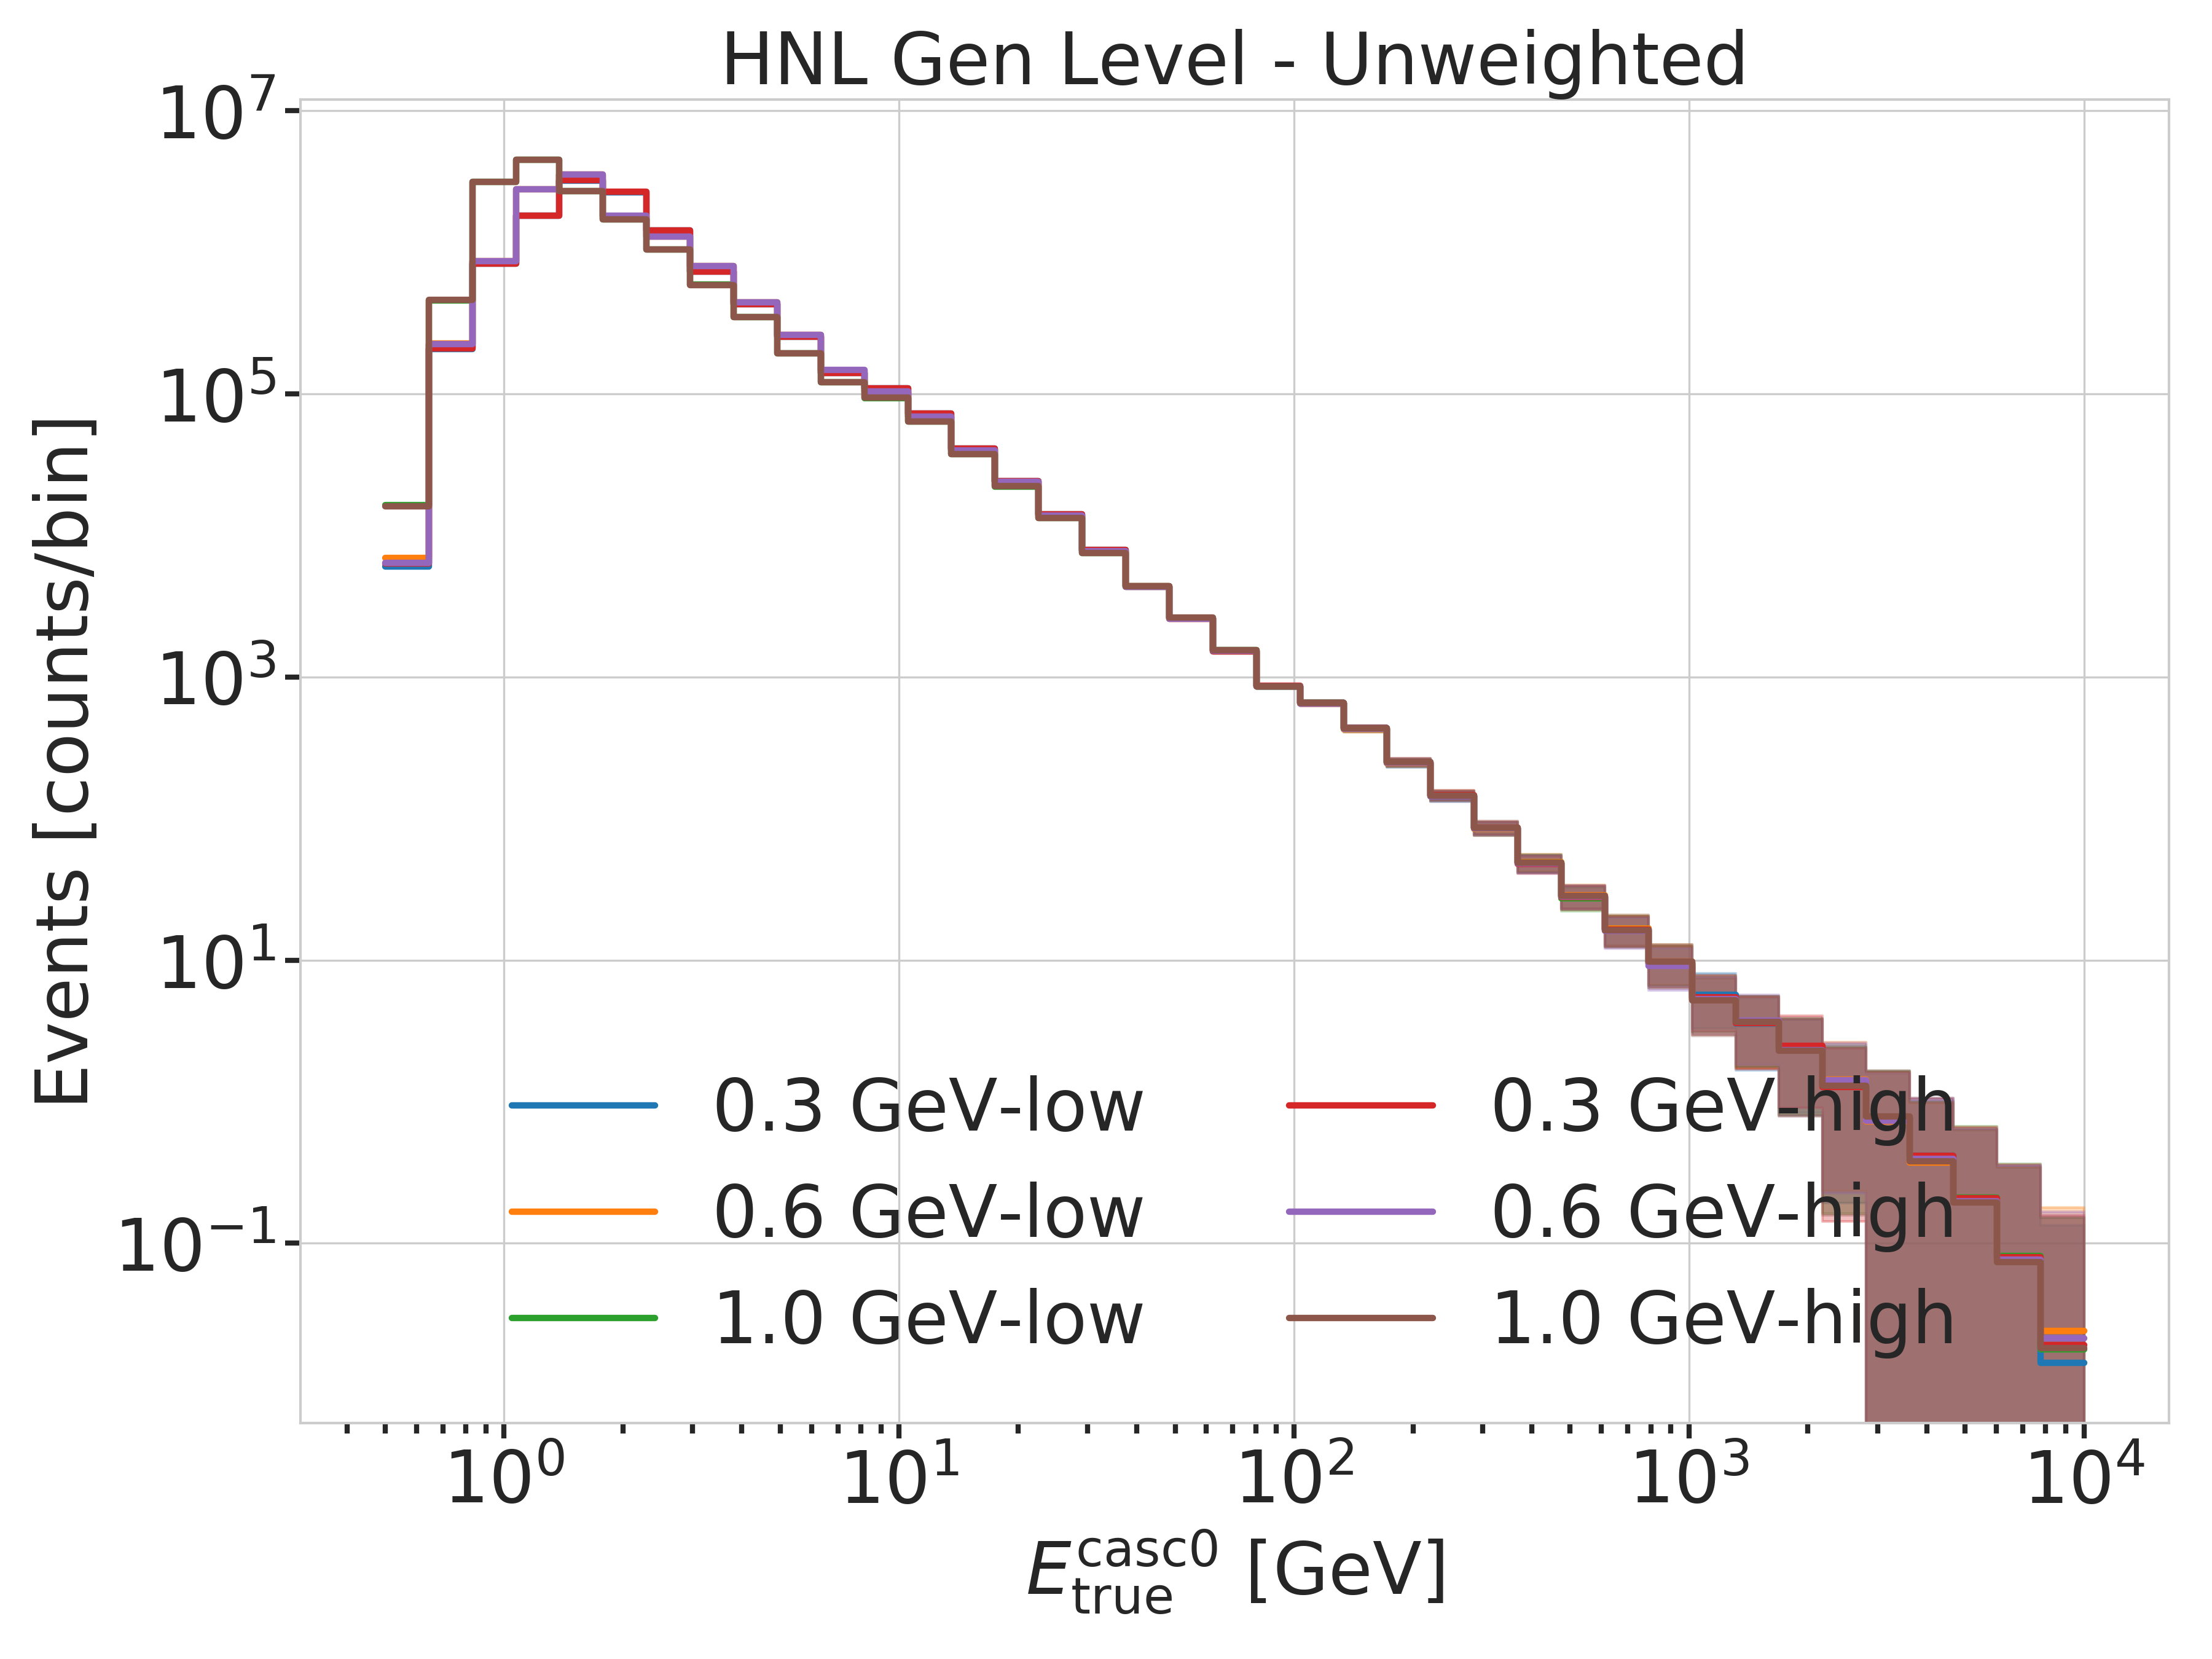
\includegraphics[width=0.49\linewidth]{figures/hnl_simulation/generation/1_d_distr_casc0_true_energy_gen_level_unweighted.png}
    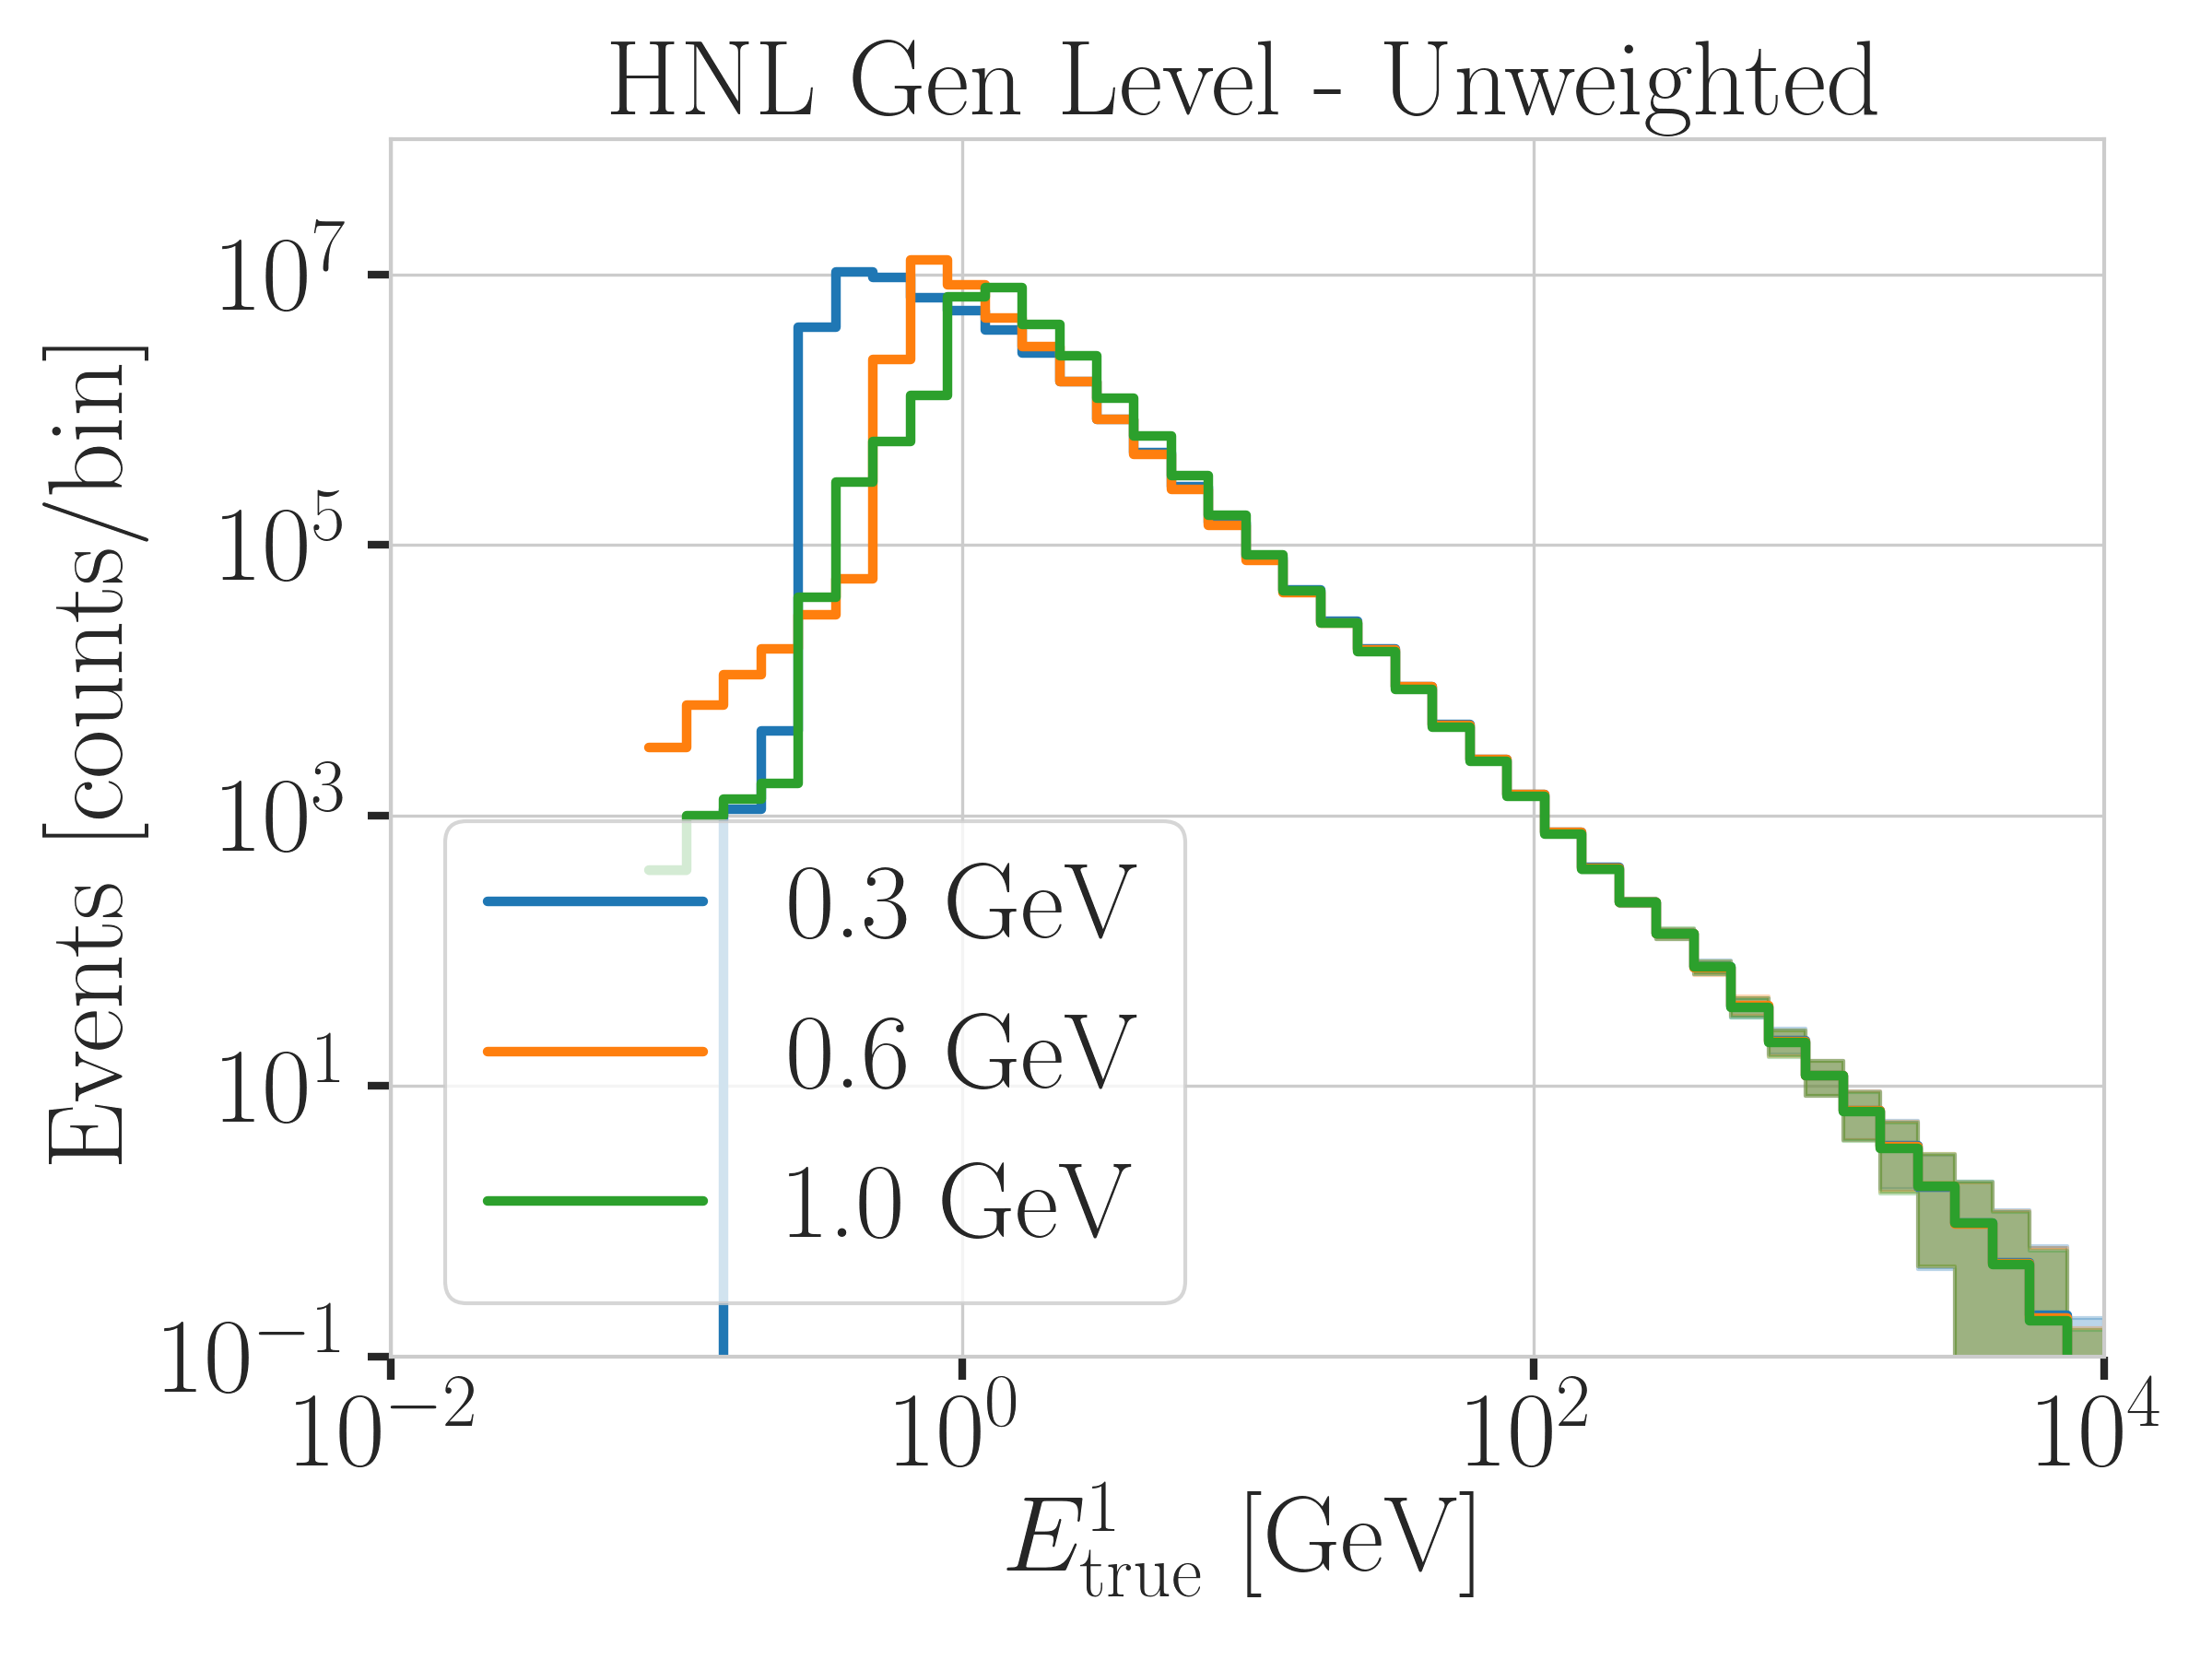
\includegraphics[width=0.49\linewidth]{figures/hnl_simulation/generation/1_d_distr_casc1_true_energy_gen_level_unweighted.png}
    \caption[Model-dependent simulation generation level distributions]{Generation level distributions of the model-dependent simulation. Shown are the true energies of both cascades including the energy that goes into invisible particles.}
    \labfig{hnl_gen_distris}
\end{figure*}


\subsection{Weighting Scheme} \labsec{hnl_weighting_scheme}

Since the lab frame decay lengths/lifetimes of the events were sampled from an inverse distribution instead of an exponential, as it would be expected from a particle decay, we have to re-weight accordingly to achieve the correct decay length distribution. The re-weighting factor is calculated as the ratio of the probability density functions PDFs of the desired exponential distribution and the inverse distribution that was sampled from as $\frac{\mathrm{PDF}_\mathrm{exp}}{\mathrm{PDF}_\mathrm{inv}}$.

The inverse distribution in the rest frame of the HNL is given by
\begin{equation}
    \mathrm{PDF}_\mathrm{inv} = \frac{1}{\tau \cdot (\ln(\tau_\mathrm{max}) - \ln(\tau_\mathrm{min}))}
    \;,
    \labeq{pdf_inverse}
\end{equation}
where $\tau$ is the rest frame lifetime and $\tau_\mathrm{min/max}$ are the minimum and maximum values of the lifetime sampling range. Since the generation range is chosen in the lab frame, the rest frame lifetime range $[\tau_\mathrm{min},\tau_\mathrm{max}]$ is defined by the lab frame decay length range $[s_\mathrm{min},s_\mathrm{max}]$ as
\begin{equation}
    \tau_\mathrm{min/max} = \frac{s_\mathrm{min/max}}{v\cdot\gamma}.
\end{equation}
Here, the gamma factor is calculated for each event as
\begin{equation}
    \gamma = \frac{\sqrt{E_\mathrm{kin}^2+m_4^2}}{m_4}
    \;,
    \labeq{gamma_factor}
\end{equation}
with the HNL mass, $m_4$, and its kinetic energy, $E_\mathrm{kin}$, while $v$ is the speed of the HNL which is calculated as
\begin{equation}
    v = c \cdot \sqrt{1 - \frac{1}{\gamma^2}}
    \;,
    \labeq{lorentz_speed}
\end{equation}
where $c$ is the speed of light.

The desired exponential distribution of the rest frame lifetime is given by
\begin{equation}
    \mathrm{PDF}_\mathrm{exp} = \frac{1}{\tau_\mathrm{proper}} \cdot e^{\frac{-\tau}{\tau_\mathrm{proper}}}
    \;,
    \labeq{pdf_exponential}
\end{equation}
where $\tau_\mathrm{proper}$ is the proper lifetime of each HNL event that is calculated using the total decay width, $\Gamma_\mathrm{total}$. Since each individual decay width calculation includes a factor of \ut4, accounting for the mixing between the HNL and the SM particles, the total decay width includes a scaling factor of \ut4. The proper lifetime is then calculated as
\begin{equation}
    \tau_\mathrm{proper} = \frac{\hbar}{\Gamma_\mathrm{total}(m_4)}
    \;,
    \labeq{proper_lifetime}
\end{equation}
where $\hbar$ is the reduced Planck constant.

This re-weighting factor is then calculated as
\begin{equation}
    w_\mathrm{lifetime} = \frac{\mathrm{PDF}_\mathrm{exp}}{\mathrm{PDF}_\mathrm{inv}} = \frac{\Gamma_\mathrm{total}(m_4)}{\hbar} \cdot \tau \cdot (\ln(\tau_\mathrm{max}) - \ln(\tau_\mathrm{min})) \cdot e^{\frac{-\tau}{\tau_\mathrm{proper}}}
    \;.
    \labeq{weight_lifetime}
\end{equation}
Adding a factor of $|U_{\tau4}|^2$ to account for the mixing at the interaction vertex the total re-weighting factor becomes
\begin{equation}
    w_\mathrm{total} = |U_{\tau4}|^2 \cdot w_\mathrm{lifetime}
    \;.
    \labeq{weight_full}
\end{equation}
If this additional weighting factor is multiplied to the generation weight introduced in \refsec{model_specific_simulation} (in \si{\meter^2}), the livetime (in \si{\second}), and the oscillated primary neutrino flux (in \si{\meter^{-2}\second^{-1}}) it results in the number of expected events in the detector for this particular MC event for a specific mixing (and mass). The only required input is therefore the mixing strength $|U_{\tau4}|^2$, since the mass is fixed for each sample. This re-weighting scheme allows to continuously vary the mixing strength and to estimate the expected event rate, which will be crucial for the analysis performed in \refch{analysis}.


\section{Standard Model Event Generation} \labsec{sm_event_generation}


\subsection{Neutrinos} \labsec{neutrino_generation}

The simulation volume is a cylinder centered in DeepCore with radius and height chosen such that all events possibly producing a signal are contained. The different sizes, chosen depending on energy and neutrino flavor, are shown in \reftab{genie_sampling_cylinder}.
\begin{table}
    \begin{center}
        \footnotesize
        \begin{tabular}{ l l l l l l }

            \hline\hline

            \textbf{Flavor} & \textbf{Energy [\si{\gev}]} & \textbf{Radius [\si{\metre}]} & \textbf{Length [\si{\metre}]} & \textbf{Events/File}  & \textbf{Files}\\ 

            \hline\hline

            \multirow{4}{*}[-1.em]{ $\nu_e+\bar{\nu_e}$ }
            & 1-4
            & \multirow{1}{*}[-1.em]{ 250 }
            & \multirow{1}{*}[-1.em]{ 500 }
            & 450000
            & \multirow{4}{*}[-1.em] {650} \\

            \cmidrule{2-2}
            \cmidrule{5-5}
            
            & 4-12
            & 
            & 
            & \multirow{1}{*}[-1.em] { 100000 }
            & \\

            \cmidrule{2-4}

            & 12-100
            & 350
            & 600
            & 
            & \\

            \cmidrule{2-5}

            & 100-10000
            & 550
            & 1000
            & 57500
            & \\

            \hline
            \hline

            \multirow{4}{*}[-1.em]{ $\nu_\mu+\bar{\nu_\mu}$ }
            & 1-5
            & 250
            & 500
            & 408000
            & \multirow{4}{*}[-1.em] {1550} \\

            \cmidrule{2-5}
            
            & 5-80
            & 400
            & 900
            & 440000
            & \\

            \cmidrule{2-5}

            & 80-1000
            & 450
            & \multirow{1}{*}[-1.em] { 1500 }
            & 57500
            & \\

            \cmidrule{2-3}
            \cmidrule{5-5}

            & 1000-10000
            & 550
            &
            & 6700
            & \\

            \hline
            \hline

            \multirow{4}{*}[-1.em]{ $\nu_\tau+\bar{\nu_\tau}$ }
            & 1-4
            & \multirow{1}{*}[-1.em]{ 250 }
            & \multirow{1}{*}[-1.em]{ 500 }
            & 1500000
            & \multirow{4}{*}[-1.75em] {350} \\

            \cmidrule{2-2}
            \cmidrule{5-5}
            
            & 4-10
            & 
            & 
            & 300000
            & \\

            \cmidrule{2-5}

            & 10-50
            & 350
            & 600
            & 375000
            & \\

            \cmidrule{2-5}

            & 50-1000
            & 450
            & 800
            & 200000
            & \\

            \cmidrule{2-5}

            & 1000-10000
            & 550
            & 1500
            & 26000
            & \\

            \hline

        \end{tabular}
    \end{center}
    \caption[GENIE generation cylinder volumes]{Cylinder volumes used for GENIE neutrino simulation generation. Cylinder is always centered in DeepCore at $(x,y,z) = (46.29,-34.88,-330.00)$ \si{\metre}.}\labtab{genie_sampling_cylinder}
\end{table}
The directions of the neutrinos are sampled isotropically and the energies are sampled from an $E^{-2}$ power law. The number of simulated events is chosen such that the livetime is more than \SI{70}{years} for each flavor. Neutrinos and antineutrinos are simulated with ratios of 70\% and 30\%, respectively, which is roughly the ratio expected from the atmospheric neutrino flux~\sidecite{PhysRevD.92.023004_Honda_Flux}.

To simulate the neutrino interaction with the ice, the \textsc{Genie} event generator~\cite{genie} (version 2.12.8) is used, resulting in the secondary particles and the kinematic and cross-section parameters. The GRV98LO PDFs were used as inputs, and the propagation of the secondary particles and of the shower development is performed identical to the description in \refsec{custom_leptoninjector} and produces the energy losses and event morphologies introduced in \refsec{icecube_propagation}.


\subsection{Muons}

Atmospheric muons are generated on a cylinder surface enclosing the full IceCube detector array. The cylinder has a height of \SI{1600}{\meter} and a radius of \SI{800}{\meter}. The energy is sampled from an $E^{-3}$ power law while the other sampling distributions (position, direction) are found from parameterizations based on~\sidecite{muon_parameterization}. This work uses full \textsc{Corsika}~\cite{corsika} simulations of muons to tailor the parameterizations, starting from \textit{cosmic ray (CR)} interactions with atmospheric nuclei using the CR flux model from~\sidecite{gaisser_cosmic_ray} and producing the muons applying the hadronic interaction model SIBYLL 2.1~\sidecite{sibyll_hadronic}. After the generation, they are propagated through the ice with PROPOSAL producing photons, treating them exactly like the muons produced in the HNL and neutrino event generation.

Since the offline processing and selection steps described in \refsec{event_selection} and \refsec{reconstruction} reduce the muon contamination to an almost negligible level, the statistical uncertainty on the number of expected muon events at the final selection level is large and therefore two separate samples of muon simulation are produced. \textbf{A first sample} is used to tune the lower level selection (up to Level 4), therefore including all events resulting from the above described generation. \textbf{A second sample} is then produced to estimate the muon contamination at higher levels (above Level 5). It only consists of muon events that pass through a smaller cylinder centered in DeepCore (height of \SI{400}{\meter} and radius of \SI{180}{\meter}), and additionally rejects events based on a KDE estimated muon density at Level 5 (in energy and zenith). This increased the simulation efficiency at Level 5 significantly, making it feasable to use this sample to estimate the muon contamination at higher levels.


\section{Detector Simulation} \labsec{detector_simulation}

The detector simulation is performed after the event generation, where the initial particles and the resulting photons and secondary particles from their propagation were produced. This part of the simulation chain is applied to all muon and neutrino simulation as well as the HNL signal simulation. The detector simulation can be split into two parts: the propagation of the photons and the simulation of the detector response (including internal noise).


\subsection{Photon Propagation} \labsec{photon_propagation}

Any photon that was produced in the event generation is individually traced through the ice, simulating scattering and absorption processes. The propagation is done using \textsc{clsim}~\cite{clsim} which is an implementation of the \textit{Photon Propagation Code (\textsc{PPC})}~\sidecite{ppc} in \textsc{OpenCL}. It is optimized to be run efficiently on GPUs. The ice is modeled as a set of \SI{10}{\meter} thick, almost horizontal layers with specific absorption and scattering lengths. The \textit{South Pole ice (SPICE)} model~\sidecite{spice_ice_model} accounts for the layers being tilted by a small amount, due to the uneven surface of the bedrock below the glacier, and the absorption and scattering lengths having a non-uniformity with respect to the azimuth direction. \reffig{simulation_ice_model} shows the values of this model for the different depths, indicating the location of IceCube, DeepCore, and the dust layer.

\begin{figure}[h]
    \begin{tikzpicture}
\pgfplotsset{set layers}

\pgfplotstableread{figures/icecube_deepcore/spice/icemodel.dat}\table

\begin{axis}[
    tab_blue,
    y axis line style={black},
    scale only axis,
    width=0.7\linewidth,
    height=0.5\linewidth,
    xmin=1100,xmax=2900,
    xticklabel style={/pgf/number format/.cd,1000 sep={}},
    axis y line*=left, % the '*' avoids arrow heads
    axis x line=none,
    ymin=0,
    enlarge y limits=true,
    xlabel=depth {[m]},
    ylabel=scattering length {[m]},
]

    \addplot[tab_blue, thick] table [x index=0, y expr=1 / \thisrowno{1}] \table;

    % dust layer
    \draw [name path=dust layer top, gray, thin] (1970, \pgfkeysvalueof{/pgfplots/ymin}) -- (1970, \pgfkeysvalueof{/pgfplots/ymax});
    \draw [name path=dust layer bottom, gray, thin] (2080, \pgfkeysvalueof{/pgfplots/ymin}) -- node[near end, sloped, above, black, font=\footnotesize\sffamily] {dust layer} (2080, \pgfkeysvalueof{/pgfplots/ymax});
    \addplot [gray, opacity=0.4] fill between [of=dust layer top and dust layer bottom];

    % IceCube
    \draw [name path=icecube top, gray, thin] (1450, \pgfkeysvalueof{/pgfplots/ymin}) -- (1450, \pgfkeysvalueof{/pgfplots/ymax});
    \draw [name path=icecube bottom, gray, thin] (1970, \pgfkeysvalueof{/pgfplots/ymin}) -- (1970, \pgfkeysvalueof{/pgfplots/ymax});
    \node[anchor=south, black, font=\footnotesize\sffamily] at (1750, 110) {IceCube\strut};
    \addplot [gray, opacity=0.2] fill between [of=icecube top and icecube bottom];

    % DeepCore
    \draw [name path=deepcore top, gray, thin] (2080, \pgfkeysvalueof{/pgfplots/ymin}) -- (2080, \pgfkeysvalueof{/pgfplots/ymax});
    \draw [name path=deepcore bottom, gray, thin] (2450, \pgfkeysvalueof{/pgfplots/ymin}) -- (2450, \pgfkeysvalueof{/pgfplots/ymax});
    \node[anchor=south, black, font=\footnotesize\sffamily] at (2270, 110) {DeepCore\strut};
    \addplot [gray, opacity=0.1] fill between [of=deepcore top and deepcore bottom];

\end{axis}

\begin{axis}[
    tab_orange,
    scale only axis,
    width=0.7\linewidth,
    height=0.5\linewidth,
    xmin=1100,xmax=2900,
    axis y line*=right,
    axis x line=none,
    ymin=0,
    enlarge y limits=true,
    ylabel=absorption length {[m]},
]

    \addplot[tab_orange, thick] table [x index=0, y expr=1 / \thisrowno{2}] \table;

\end{axis}

\begin{axis}[
    scale only axis,
    width=0.7\linewidth,
    height=0.5\linewidth,
    xmin=1100,xmax=2900,
    xticklabel style={/pgf/number format/.cd,1000 sep={}},
    axis y line*=left, % the '*' avoids arrow heads
    xlabel=depth {[m]},
    axis y line=none,
]

\addplot[tab_orange, thick] table [x index=0, y expr=1 / \thisrowno{2}] \table;


\end{axis}

\end{tikzpicture}

	\caption[Depth dependent scattering and absorption lengths]{Scattering and absorption lengths as a function of depth in the SPICE model used for simulation. Modified from~\cite{ATrettin_phd}.}
    \labfig{simulation_ice_model}
\end{figure}

In an initial step, each photon's absorption length is sampled from an exponential distribution with the expectation value at the current layer's absorption length. The following propagation steps are performed in parallel for all photons. In each of those steps, corresponding to a single scattering event, the photon travels a length that is sampled from an exponential distribution with the expectation value at the scattering length of the current layer and the scattering angle chosen based on a combination of a simplified Mie scattering distribution~\sidecite{mie_scattering} and a Henyey-Greenstein distribution~\sidecite{henyey_greenstein, ice_calibration}. The parameters defining the shape of these distributions were calibrated using data from \textit{in-situ} LED calibration runs. These steps are continuously repeated until each photon reaches a DOM or is absorbed\sidenote{A photon is absorbed, when it traveled its full absorption length, sampled in the initial step of the photon propagation.}. After all photons have been propagated in that manner, the final step is to store the photons that reached a DOM for further processing.


\subsection{Detector Responses}

The second part of simulating the IceCube detector is the DOM response. For a photon that reaches a DOM, the probability to produce a signal depends on the total efficiency and the angular acceptance of the specific DOM. The total efficiency includes effects of the DOM glass, PMT quantum and photo-electron collection efficiencies, and it is wavelength dependent. Additionally, there is another angle dependent effect called \textit{hole ice}~\sidecite{Fiedlschuster:2019unl}. This effect is due to varied ice properties resulting from the re-freezing process of the water column inside the borehole after deployment of the string. Accepted photons are converted into a so-called \textit{Monte Carlo photo-electron (MCPE)}. The amount of charge measured for each MCPE is determined by sampling from the \textit{single photo-electron (SPE)} distribution, which was tuned to match the observed distribution in each DOM in an \textit{in-situ} calibration study~\sidecite{spe_respose_pmt}. \reffig{spe_distribution} shows the spread of the distribution measured over all DOMs compared to lab measurements of a specific PMT type. Based on the sampled charges and times of MCPEs, the voltage waveforms for the (two) different readout channels are simulated and passed on to the trigger simulation starting with WaveDeform (see \refsec{ice_and_DOMs}).

\begin{margintable}
\small
    \begin{tabular}{ ll }
    \hline\hline

    \textbf{Parameter} & \textbf{Value} \\ 

    \hline\hline

    Therm. rate $\lambda_\mathrm{th}$ & $\SI{180}{\hertz}$ \\
    Decay rate $\lambda_\mathrm{dec}$ & $\SI{80}{\hertz}$ \\
    Decay hits $\eta$ &  $8.5$ \\
    Decay $\mu$ & 4.3 $\log_{10}$(\si{\nano\second}) \\
    Decay $\sigma$ & 1.8 $\log_{10}$(\si{\nano\second}) \\

    \hline
    \end{tabular}
\caption[Vuvuzela noise simulation parameters]{Typical parameter values used in the vuvuzela noise simulation. Averaged over all DOMs.}
\labtab{vuvuzela_parameters}
\end{margintable}

\begin{figure}[h]
    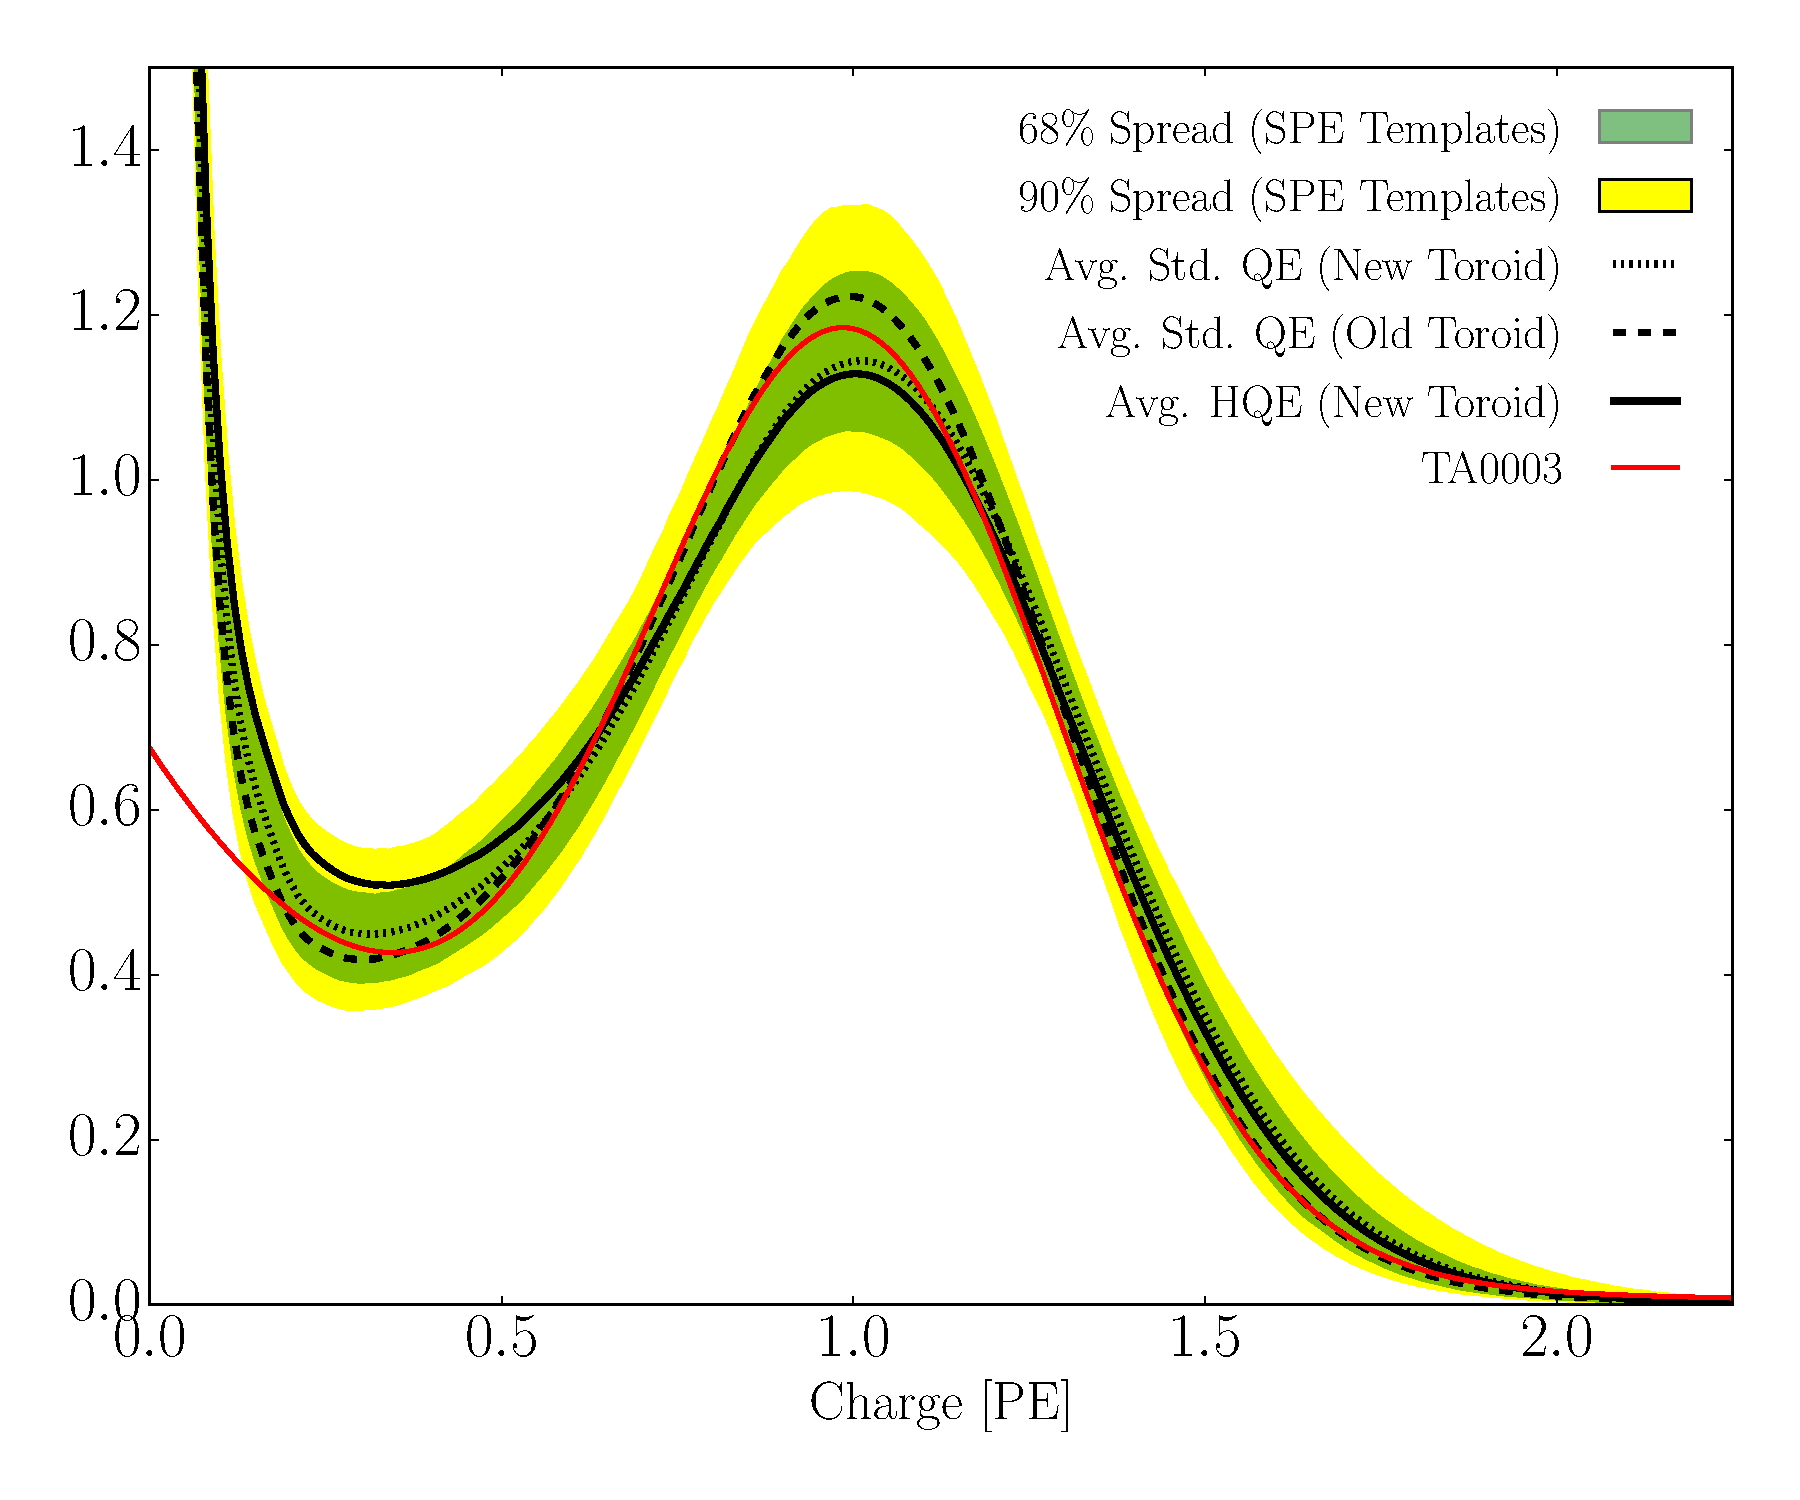
\includegraphics[width=.9\textwidth]{figures/simulation_and_processing/SPE_TA003_2.pdf}
	\caption[Single photo-electron charge distribution]{Single photo-electron charge distribution shown for a lab measurement in red (TA0003), various hardware configurations in black dashed, dotted, and solid lines, and the \SI{68}{\percent} and \SI{90}{\percent} spread of the measured charged templates for all DOMs. All curves are normalized to the same area. The figure is taken from~\cite{spe_respose_pmt}.}
    \labfig{spe_distribution}
\end{figure}

Besides the Cherenkov photons, IceCube also observes photons that are produced in radioactive decays inside the DOMs, both in the glass housing sphere and the PMT glass itself. To simulate this internal noise, the \emph{Vuvuzela} module~\sidecite{MLarson_master, MLarson_phd} is used to create additional MCPEs that are fed into the same simulation chain described above. The noise hits are simulated by drawing the times from a constant rate Poisson process and the number of photons from a Poisson distribution. Then the time differences between the individual photons per hit is found, based on a Log-Normal distribution. The simulation is defined by 5 parameters that are calibrated for each DOM individually. \reftab{vuvuzela_parameters} shows the average values for these parameters.


\setchapterstyle{kao}
\setchapterpreamble[u]{\margintoc}


\chapter{Event Processing and Reconstruction}
\labch{simulation_and_processing}

The analysis presented in this thesis is highly dependent on an efficient filtering and event selection to reduce the raw IceCube trigger data to a usable atmospheric neutrino sample. Based on this selection, a precise estimation of both expected SM background and expected BSM signal events can be made using MC simulations. Starting from the PMT output, both data and simulation are processed through the in-ice trigger, the online filter and processing, and the low-energy event selection to produce a neutrino dominated sample. Once the sample is small enough for more sophisticated reconstruction techniques to be feasible to run, the events can be reconstructed with the existing IceCube reconstruction algorithms. At this level it is also possible to test and develop new reconstruction algorithms, without complications due to the large amount of background events from atmospheric muons and noise that are present before the filtering.

After describing the processing and filtering chain in \refsec{processing_chain}, the development and performance of a dedicated low-energy double-cascade reconstruction algorithm is presented in \refsec{dc_reconstruction}. Based on the results from this reconstruction, the ability of the detector to observe and identify double-cascades is discussed in \refsec{dc_classification}. Finally, the state-of-the-art SM neutrino event reconstruction is presented in \refsec{reconstruction}, which is used to perform the analysis in this thesis.


\section{Processing} \labsec{processing_chain}

After the detector simulation is performed, all MC and data are processed in exactly the same way. This section explains the trigger and event selection that is applied starting from the raw voltage measured by the PMTs. It is split in different steps that are run inside the ice, at the South Pole, and after the data was transferred to the North\sidenote{Since the IceCube detector is at the South Pole, the data storage and processing sites in the Northern Hemisphere are shortly referred to as \textit{the North}.}. The complexity and computational cost of the processing increases with each step, while the total number of events reduces, making it feasible and reducing the use of computational resources on events that are not of interest for analyses. 


\subsection{Trigger and Filter} \labsec{trigger_and_filter}

Before the data can be sent to the North, the initial signal coming from the PMT is a voltage waveform that is digitized (for data) and then information of photon hits are extracted (also for the MC coming from the detector response simulation). The trigger and filter explained here are tailored to select events that pass through the DeepCore volume, while rejecting background events (either from atmospheric muons or from random noise). There are other filters used in IceCube which will not be explained here, since they are not relevant for this work. A full description of the instrumentation and the online systems can be found in~\sidecite{Aartsen:2016nxy}.


\subsubsection{In-ice Trigger} \labsec{trigger}

The trigger is applied inside the DOM in the ice before sending the information to the ICL on the surface. The time dependent voltage curves are captured if a pre-defined threshold value is exceeded. Once the threshold, set to the equivalent of \SI{0.25}{PE}, is crossed, \SI{6.4}{\micro\second} of the waveform are coarsely digitized by a \textit{Fast Analog-to-Digital Converter (FADC)} with a sampling rate of \SI{40}{\mega\hertz}. Additionally, the first \SI{427}{\nano\second} are digitized using an \textit{Analog Transient Waveform Recorder (ATWD)} with a sampling rate of \SI{300}{\mega\hertz}~\sidecite{ABBASI2009294_data_acquisition}, but only if some trigger condition is met, because this readout frequency is too high to be sampled directly and requires some buffering. For DeepCore, the HLC condition already mentioned in \refsec{ice_and_DOMs} has to be met for three DOMs inside the fiducial volume within a time window of \SI{5}{\micro\second}. If this is the case, all waveforms that crossed the threshold within a \SI{20}{\micro\second} time window around the trigger are digitized and sent to the ICL for further processing. This trigger is called DeepCore \textit{Simple Multiplicity Trigger 3 (SMT-3)}. The DOM hits that are read out in this process, but do not meet the HLC condition, are called \textit{soft local coincidence (SLC)} hits. The rate of the DeepCore SMT-3 trigger is $\sim$\SI{250}{\hertz}~\cite{2017JInst..12P3012A_Instrumentation_Systems}.


\subsubsection{Online Filter} \labsec{online_filter}

The digitized waveforms are sent to the ICL, where a further filter is applied \textit{online}\sidenote{Where \textit{online} means running on hardware at the South Pole as opposed to \textit{offline} at the IceCube institutions in the Northern Hemisphere.}. First, the WaveDeform algorithm is run to extract photon arrival times and charge from the waveforms. Next, the DeepCore filter is applied, which is an iterative hit cleaning starting from HLC hits and removing any hits outside a \SI{125}{\meter} radius and a \SI{500}{\nano\second} time window (called \textit{radius-time cleaning (RT-cleaning)}) of the initial hit. This mainly rejects unphysical SLC hits, which are potentially caused by random noise. All following selection steps are done using the resulting cleaned pulses.

An additional cut is applied to reject events that are likely to be caused by atmospheric muons. This is done by splitting the hits depending on whether they were inside the DeepCore fiducial volume or outside and then calculating the speed of each hit outside the fiducial volume towards the \textit{center of gravity (COG)} of the hits inside. If one of them has a speed close to the speed of light, the whole event is rejected, because this is a strong indication for a muon event.

As input for the further selection levels, several event properties, such as vertex position and direction, are determined using fast and simple event reconstructions. After the DeepCore online filter is applied, the data rate is about \SI{15}{\hertz}, which can be sent to the North via satellite for further processing.


\subsection{Event Selection} \labsec{event_selection}

After the data was sent to the North, the \textit{offline} filters and selections are applied to further reduce the background of atmospheric muons and noise. The selection is split into three levels referred to as \textit{Level 3-5 (L3-L5)}, which bring down the muon rate to $\sim$\SI{1}{\milli\hertz}, while the remaining fraction of random noise is below \SI{1}{\percent}. The neutrino rate after this level is \SI{2}{\milli\hertz}, making it a neutrino dominated sample. Assuming a HNL mass of \SI{0.6}{\gev} and a mixing of 0.1, the expected rate of HNL events after the selection is $\sim$\SI{5}{\micro\hertz}. A more detailed investigation of the HNL selection efficiency is presented in \refsec{dc_reconstruction_performance}.


\subsubsection{Level 3} \labsec{level_3}

At the first offline filtering level, Level 3, one-dimensional thresholds are used to reduce atmospheric muons, pure noise, and coincident muons. This selection is targeting regions where the data/MC agreement is poor, so that more sophisticated \textit{machine learning (ML)} techniques can be applied at later levels. The selection is made using 12 control variables, that are inexpensive to compute for the very large sample at this stage. The variables are related to position, time, and overall number of hits in the event.

Pure noise hits, that are temporally uncorrelated, are cleaned by applying a \SI{300}{\nano\second} sliding window, requiring the containment of more than 2 hits at its maximum. Additionally, an algorithm is run to check whether the hits show some directionality, accepting them only if they do.

To reduce the amount of muons a series of thresholds is applied using spatial and temporal information. Events that have more than 9 hits observed above \SI{-200}{\meter} or the first HLC hit above \SI{-120}{\meter} are rejected as well as events where the fraction of hits in the first \SI{600}{\nano\second} of the event is above 0.37, ignoring the first two hit DOMs. Additionally, the ratio between hits in the veto region and the DeepCore fiducial volume is required to be below 1.5.

If a muon enters the detector after the data acquisition was already triggered, it causes events that span over a much larger time range. To reduce those coincident events, the time difference between first and last pulse cannot be above \SI{5000}{\nano\second}. This cut mainly affects a region of very poor data to MC agreement, because coincident events are not simulated at all.

The L3 selection removes \SI{95}{\percent} of the atmospheric muons and >\SI{99}{\percent} of pure noise hits, while keeping >\SI{60}{\percent} of the neutrino events. The sample now roughly contains muons/neutrinos/noise at a ratio of 100:10:1 with a total rate of $\sim$\SI{0.5}{\hertz}.


\subsubsection{Level 4} \labsec{level_4}

After the total rate was reduced by the simple selection criteria at L3 and the overall agreement between data and MC is established, ML techniques can be applied to further reduce the background. For Level 4, two \textit{Boosted Decision Trees (BDTs)}~\sidecite{BDT} classifiers are trained to separate neutrino events from atmospheric muons and noise hits, separately. The output of each classifier, a probability score, can be seen in \reffig{level_4_classifiers}. The noise filter is applied first and an event passes, if the score is larger than 0.7, reducing the noise hits by a factor of 100, while keeping \SI{96}{\percent} of neutrinos. Then the second BDT classifier is applied to reject muons. It was trained partly on unfiltered data, which consists of >\SI{99}{\percent} atmospheric muons, to reject the data and keeping the neutrinos from the simulation. Rejecting events with a score smaller than 0.65 removes \SI{94}{\percent} of atmospheric muons while keeping \SI{87}{\percent} of neutrinos. After applying the L4 selection, based on the BDT classifier outputs, the sample is still dominated by atmospheric muons, while the noise rate dropped to below most neutrino types.

\begin{figure*}
\centering 
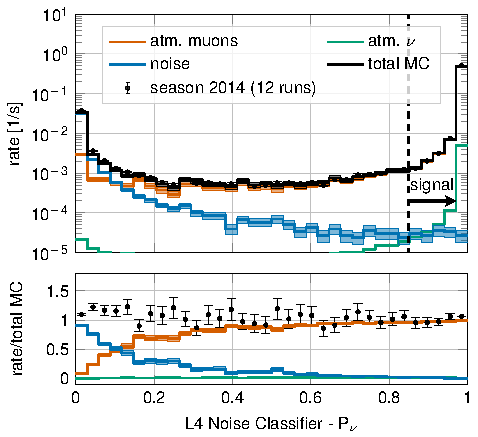
\includegraphics[width=0.49\linewidth]{figures/simulation_and_processing/selection/l4_noise_classifier_probnu.pdf}
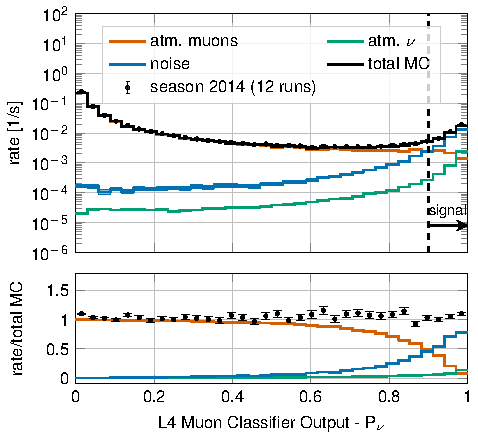
\includegraphics[width=0.49\linewidth]{figures/simulation_and_processing/selection/l4_muon_classifier_probnu.pdf}

\caption[Level 4 classifier outputs (muon and noise)]{Distributions of Level 4 noise classifier output (left) and muon classifier output (right), where larger values indicate more neutrino-like and lower values more noise-like/muon-like. Taken from~\cite{OVS_PRD}.}
\labfig{level_4_classifiers}
\end{figure*}


\subsubsection{Level 5} \labsec{level_5}

Level 5 is the final selection level, before event reconstructions are applied. This level aims to reduce the remaining atmospheric muon rate below the rate of neutrinos. Muons not rejected by the earlier levels are those that produced little or no light in the veto regions. One possible reason is that they passed through one of the uninstrumented regions between the strings called \textit{corridors}. To reject those, special corridor selection criteria are applied, which are based on the number of hits the event produced close to a potential corridor it passed through. The potential corridor in questions is identified based on a simple infinite track fit. In addition to the corridor selection, starting containment conditions are applied to reject events that start at the edge of the fiducial volume. Events with more than seven hits in the outermost strings of the detector or those that have a down-going direction in the uppermost region are rejected. This further reduces the fraction of muons by \SI{96}{\percent} while keeping \SI{48}{\percent} of neutrinos.


\section{Double-Cascade Reconstruction} \labsec{dc_reconstruction}

In the energy range relevant for this work, around 10s of \si{\gev}, the light deposition is very low and only a few DOMs detect photons, making event reconstructions difficult. Existing reconstruction algorithms applied for low-energy atmospheric neutrino events are either assuming a single-cascade hypothesis or a track and cascade hypothesis, which are the two SM morphologies observable at these energies, as was described in \refsec{icecube_signatures}. A HNL being produced and decaying inside the IceCube detector however, will produce two cascade-like light depositions. The morphology, spatial separation between the cascades, and their individual properties depend on the model parameters discussed in \refsec{double_cascade_morphology}. To investigate the performance of the detector to observe and identify these events, a low-energy double-cascade reconstruction algorithm was developed. It is based on a pre-existing algorithm used to search for double-cascades produced from high-energy astrophysical tau neutrinos~\sidecite{Abbasi:2020zmr} that was established in~\sidecite{PHallen, MUsner}.


\subsection{Table-Based Minimum Likelihood Algorithm}

The double-cascade reconstruction is relying on a minimum likelihood algorithm, which is the \textit{classical} approach to IceCube event reconstructions, as opposed to ML based methods. It compares the observed light depositions in the detector to the expected light depositions from a given event hypothesis, where the event hypothesis can be constructed from building blocks of single-cascade and track segment expectations. Varying the energies of the track segments and cascade components changes the light expectation and can be used to find the best fit hypothesis to the observed data. A Poissonian likelihood is constructed, which compares the observed photon numbers, $n$, with their arrival times to the expected light depositions, $\mu$, for a given event hypothesis as
\begin{equation}
    \ln(L) = \sum_j \sum_t n_{j,t} \cdot \ln(\mu_{j,t}(\Theta) + \rho_{j,t}) - (\mu_{j,t}(\Theta) + \rho_{j,t}) - \ln(n_{j,t}!)
    \;,
    \labeq{millipede_likelihood}
\end{equation}
where $\rho$ are the number of expected photons from noise, $\Theta$ are the parameters governing the source hypothesis, and the likelihood is calculated summing over all DOMs, $j$, splitting observed photons into time bins, $t$. The light expectations are calculated using look-up tables~\sidecite{photospline} that contain the results from MC simulations of cascade events or track segments. By varying the parameters defining the event hypothesis, the likelihood of describing the observed light pattern by the expected light depositions is minimized to find the reconstructed event. Algorithms of this kind, used in IceCube, are described in more detail in~\sidecite{IceCube:2013dkx}. For the table production a specific choice of ice model has to be made, while the calibrated DOM information is taken from the measurement itself.

Based on the tabulated light expectations for cascades and track segments, various hypotheses describing different event morphologies can be constructed. These are commonly the cascade only or the track and cascade hypotheses. The hypothesis describing the double-cascade signature of the HNL is using two cascades that are separated by a certain distance. The whole hypothesis is defined by 9 parameters and assumes that the two cascades are aligned with each other, which is a safe assumption for strongly forward boosted interactions and because low-energy cascades do not show a strong directionality. The parameters are the position of the first cascade, $x, y, z$, the direction of both cascades, $\phi, \theta$, and its time, $t$, as well as the decay length, $L$, between the two cascades. Assuming the speed of the HNL to be the speed of light, $c$, this already defines the full hypothesis, because the time and position of the second cascade are then fully determined by properties of the first cascade and the decay length. Note here, that the HNL particle does not produce any light while traveling, as it is electrically neutral. Since the likelihood only sums over DOMs that have observed photons, the non-observation of light is implicitly used as information and will exclude hypotheses with light expectation in those DOMs. The full 9 parameters describing an event are $\Theta = (x, y, z, t, \theta, \phi, E_0, E_1, L)$. To compute the full likelihood, the term in \refeq{millipede_likelihood}, defined for a single event hypothesis, is summed over both cascade contributions, as $\sum_i \ln(L_i)$, with $i$ being the cascade indices.


\subsection{Optimization for Low Energies}

Optimizing the double-cascade reconstruction for low-energy events was done in parallel to the development of the model-dependent simulation generator introduced in \refsec{model_specific_simulation}. A preliminary sample of HNL events from the model-dependent simulation was used, containing a continuum of masses between \SIrange[range-phrase=~and~]{0.1}{1.0}{\gev} and lab frame decay lengths sampled uniformly in the range from \SIrange{5}{500}{\meter}. Even though this sample is not representative of a physically correct model and therefore not useful to predict the event expectation, it can still be used to optimize the reconstruction. The double-cascade nature of the individual events is present and the evenly spaced decay length distribution is especially useful for the purpose of optimizing the reconstruction.

The simulation is processed up to Level 5 of the selection chain described in \refsec{event_selection} and one of the reconstructions from~\sidecite{low_energy_reco_IC} is applied to the events, fitting a cascade and a track and cascade hypothesis. The results from this reconstruction are used as an input for the double-cascade reconstruction, where the position of the vertex, the direction of the event, and its interaction time are used as the input quantities for the first cascade, and the length of the track reconstruction is used as a seed for the distance between the two cascades. Several reconstructions were tested as seeds for the vertex position and the direction, but the choice did not significantly alter the results reported here.


\subsubsection{Fit Routine}

\begin{marginfigure}
	\centering
    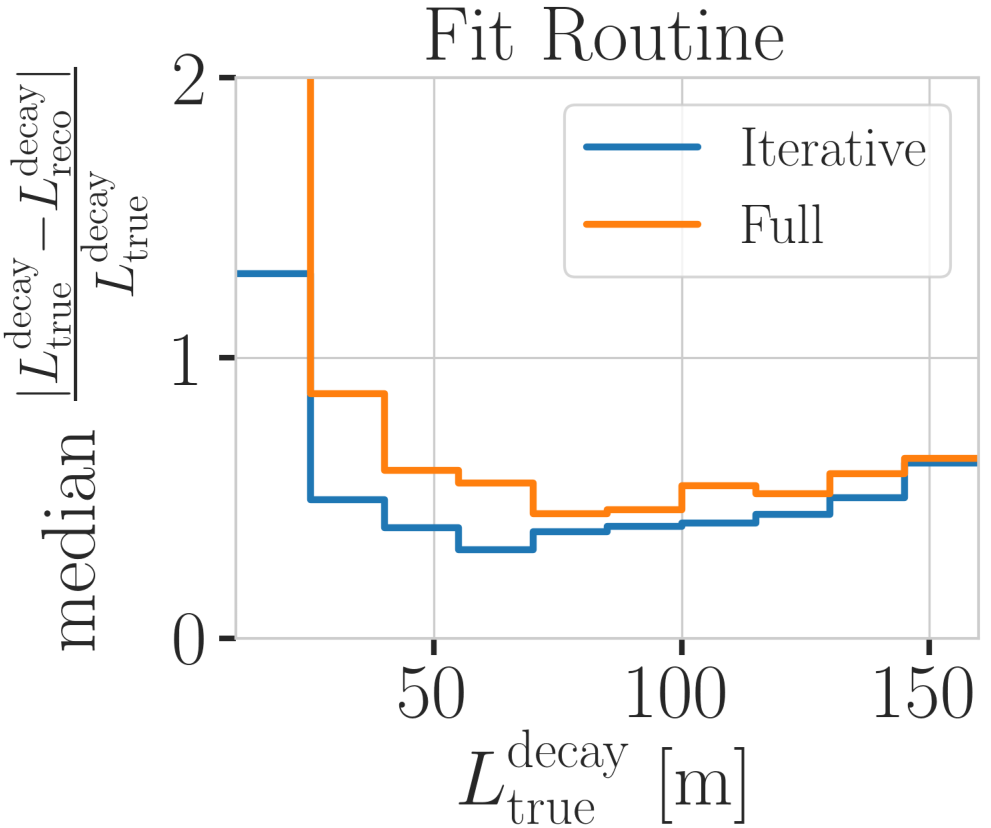
\includegraphics{figures/results/190605_reco_optimization/fit_routine_splitting_median_decay_length_resolution_Good + L7 + reco E1,E2 above 3_fix_y_new.png}
    \caption[Decay length resolution to optimize fit routine]{Decay length resolution as a function of the true decay length, comparing a full 9 parameters fit to an iterative approach where first the energies and the decay length are fit, while fixing the other 7 parameters and then the full fit is performed.}
    \labfig{fit_routine_optimization_fit_routine}
\end{marginfigure}

The full 9 dimensional likelihood space is very complex and can have many local minima, depending on the specific event and its location in the detector. For this reason, a more sophisticated fit routine than fitting all 9 parameters at once was tested. In a first fit iteration, some parameters are fixed and the resulting best fit point is used to fit all 9 parameters in a second iteration. The effect is shown in \reffig{fit_routine_optimization_fit_routine}, which shows the median of the absolute, fractional decay length error with respect to the true decay length, for the full fit and an iterative fit routine. It can be seen how a fit split into two consecutive steps, where the first step fits only both cascade energies and the decay length and the second step fits the full 9 parameters, performs better as compared to a single, full 9 parameter fit. The initial seed remains identical for both the routines.


\subsubsection{Decay Length Seeds}

\begin{marginfigure}
	\centering
    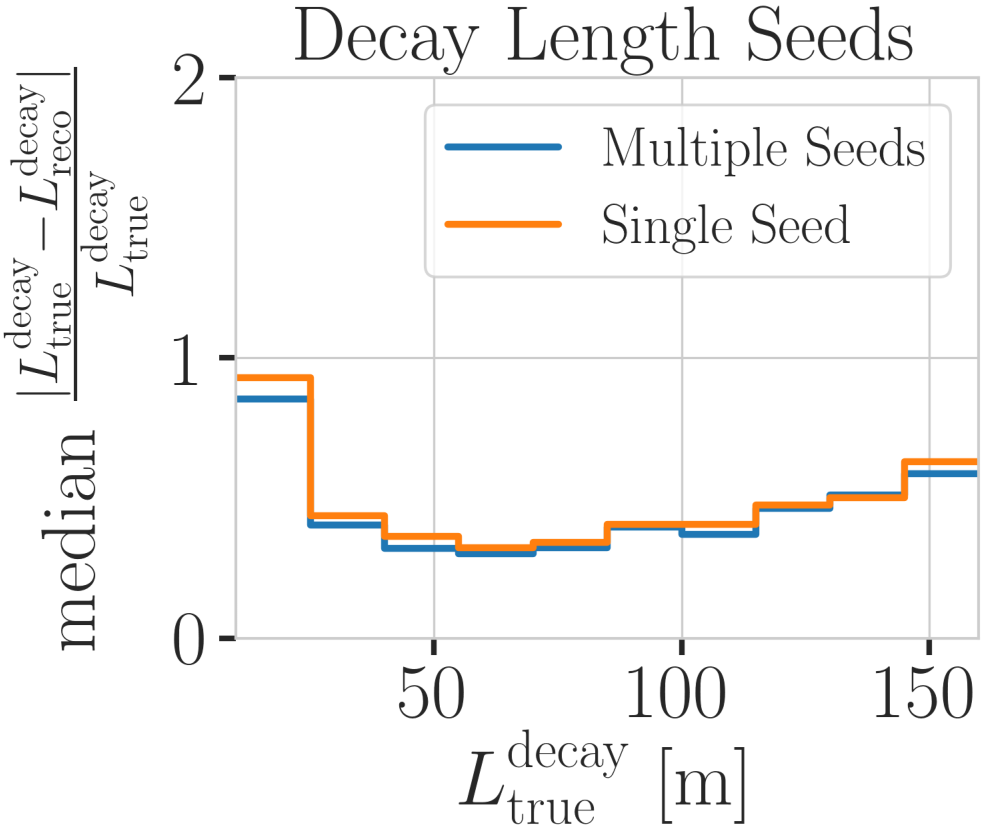
\includegraphics{figures/results/190605_reco_optimization/decay_length_seeding_median_decay_length_resolution_Good + L7 + reco E1,E2 above 3_fix_y_new.png}
    \caption[Decay length resolutions to optimize length seeding]{Decay length resolution as a function of the true decay length, comparing the same fit routine seeded with just the seed decay length and seeded with a decay length of \SI{5}{\meter}, \SI{25}{\meter}, \SI{50}{\meter}, \SI{100}{\meter}, and \SI{200}{\meter} on the left.}
    \labfig{fit_routine_optimization_decay_length_seeding}
\end{marginfigure}

From the seed values of the reconstruction, especially the length between the two cascades was found to have a very strong impact on whether the global minimum was found during the minimization. To mitigate this effect, multiple fits are performed, seeding with variations of the input length at different orders of magnitude. The best result is used, selected based on the total likelihood value of the best fit parameter set. A small improvement in the decay length resolution can be found by using this approach as compared to a single length seed. The resolutions for the differnt approaches are shown in \reffig{fit_routine_optimization_decay_length_seeding}.


\subsubsection{Minimizer Settings}

\begin{marginfigure}
	\centering
    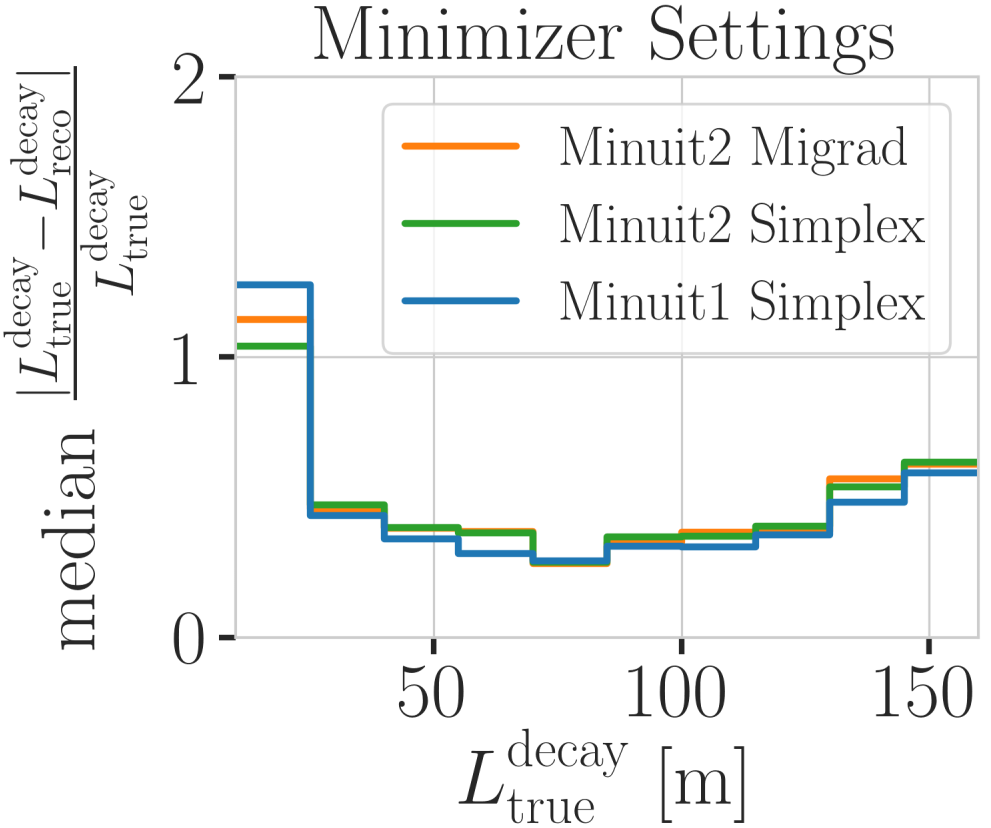
\includegraphics{figures/results/190605_reco_optimization/minimizer_checks_median_decay_length_resolution_Good + L7 + reco E1,E2 above 3_fix_y_new.png}
    \caption[Decay length resolution to optimize minimizer settings]{Decay length resolution as a function of the true decay length, comparing the same fit routine performed with different minimizers.}
    \labfig{fit_routine_optimization_minimizer_checks}
\end{marginfigure}

To investigate the effect of the minimizer used to find the best fit parameters, the reconstruction was performed using three different minimizers, which were easily accessible within the reconstruction framework. The minimizers used were Minuit1 Simplex, Minuit2 Simplex, and Minuit2 Migrad~\sidecite{og_minuit}. As can be seen in \reffig{fit_routine_optimization_minimizer_checks}, Minuit1 Simplex performed best and was chosen as the default for the reconstruction. Global minimizers may improve the performance of the reconstruction, but were not available in the framework and would require significant software development.


\subsection{Performance} \labsec{dc_reconstruction_performance}

The optimization of the reconstruction was performed using preliminary development versions of the model-dependent HNL simulation. To investigate the effect of the low-energy event selection and the double-cascade reconstruction performance in a generic way, the model-independent simulation introduced in \refsec{model_independent_simulation} is used. The important advantage of the model-independent samples is the controllable parameter space, especially in cascade energies and decay length, because the event kinematics are not coupled to the underlying HNL model, but can be chosen freely. This means that some benchmark edge cases can be investigated, and the performance can also be assessed for a realistic scenario in addition to mapping out the effects of the event selection and where the reconstruction breaks down.

\begin{margintable}
    \footnotesize
    \begin{tabular}{ ll }
    \hline\hline    
    \textbf{Type} & \textbf{Setting} \\
    \hline\hline
    Minimizer & Minuit1 Simplex \\
    $L_\rm{decay}$ seeds & $(0.5, 1.0, 1.5) \cdot L_\rm{seed}$ \\
    Fit routine & Iterative \\
    \hline
    \end{tabular}
\caption[Double-cascade reconstruction settings]{Chosen settings for the double-cascade reconstruction algorithm.}
\labtab{dc_reco_settings}
\end{margintable}

The chosen final settings and procedures used for the low-energy double-cascade reconstruction algorithm are summarized in \reftab{dc_reco_settings}. In the first fit iteration, the number of time bins in \refeq{millipede_likelihood} is set to 1, so just the number of photons and their spatial information is used. In the second step the number of time bins is chosen such that each photon falls into a separate time bin, which means all time information is used. The average runtime per event is $\sim$\SI{16}{\second} on a single CPU core, but is very dependent on the number of photons observed in the event, since the likelihood calculation in the second step scales with this number and a table lookup has to be performed for each photon.


\subsubsection{Best-Case Events}

\begin{marginfigure}
    \centering
    % [trim=left bottom right top, clip]
    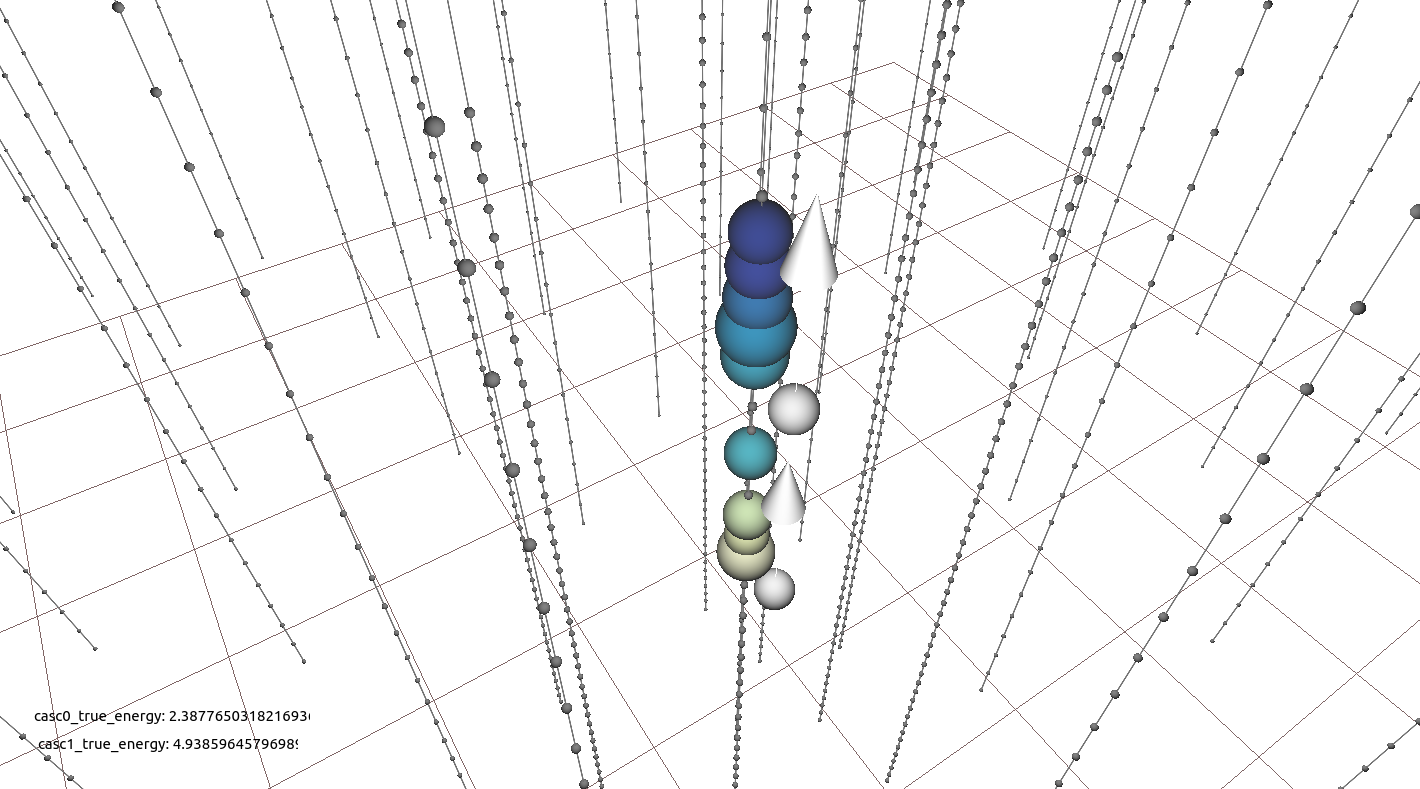
\includegraphics[trim=270 40 225 35, clip]{figures/model_independent_simulation/upgoing_e0_2.4_e1_4.9_v2.png}
    \caption[Event view of an up-going double-cascade event]{Event view of an up-going double-cascade event, with cascade energies of \SI{2.4}{\gev} and \SI{4.9}{\gev}, and a decay length of \SI{65.8}{\meter}. The colored spheres show the DOMs that have observed light, where the size is proportional to the number of observed photons and the color indicates the time (yellow is early, blue is late). The strings are shown as black lines, with small spheres indicating the DOM positions, and the true cascade vertices and directions are shown as white spheres with white arrows.}
    \labfig{up-going_example_event}
\end{marginfigure}

The best-case scenario to observe an event is to be directly on top of a string with a straight up-going direction. Using the simulation sample introduced in \refsec{simplistic_samples} and running the double-cascade reconstruction from \refsec{dc_reconstruction} on these events, it is possible to estimate the performance limit of the reconstruction. \reffig{up-going_example_event} shows one example event view from that sample, where the cascade energies are \SI{2.4}{\gev} and \SI{4.9}{\gev}, and the decay length is \SI{65.8}{\meter}. It can be seen that despite the low energies, both cascades deposit light in the DOMs and the reconstruction is expected to work.

\begin{figure*}[h]
	\centering
    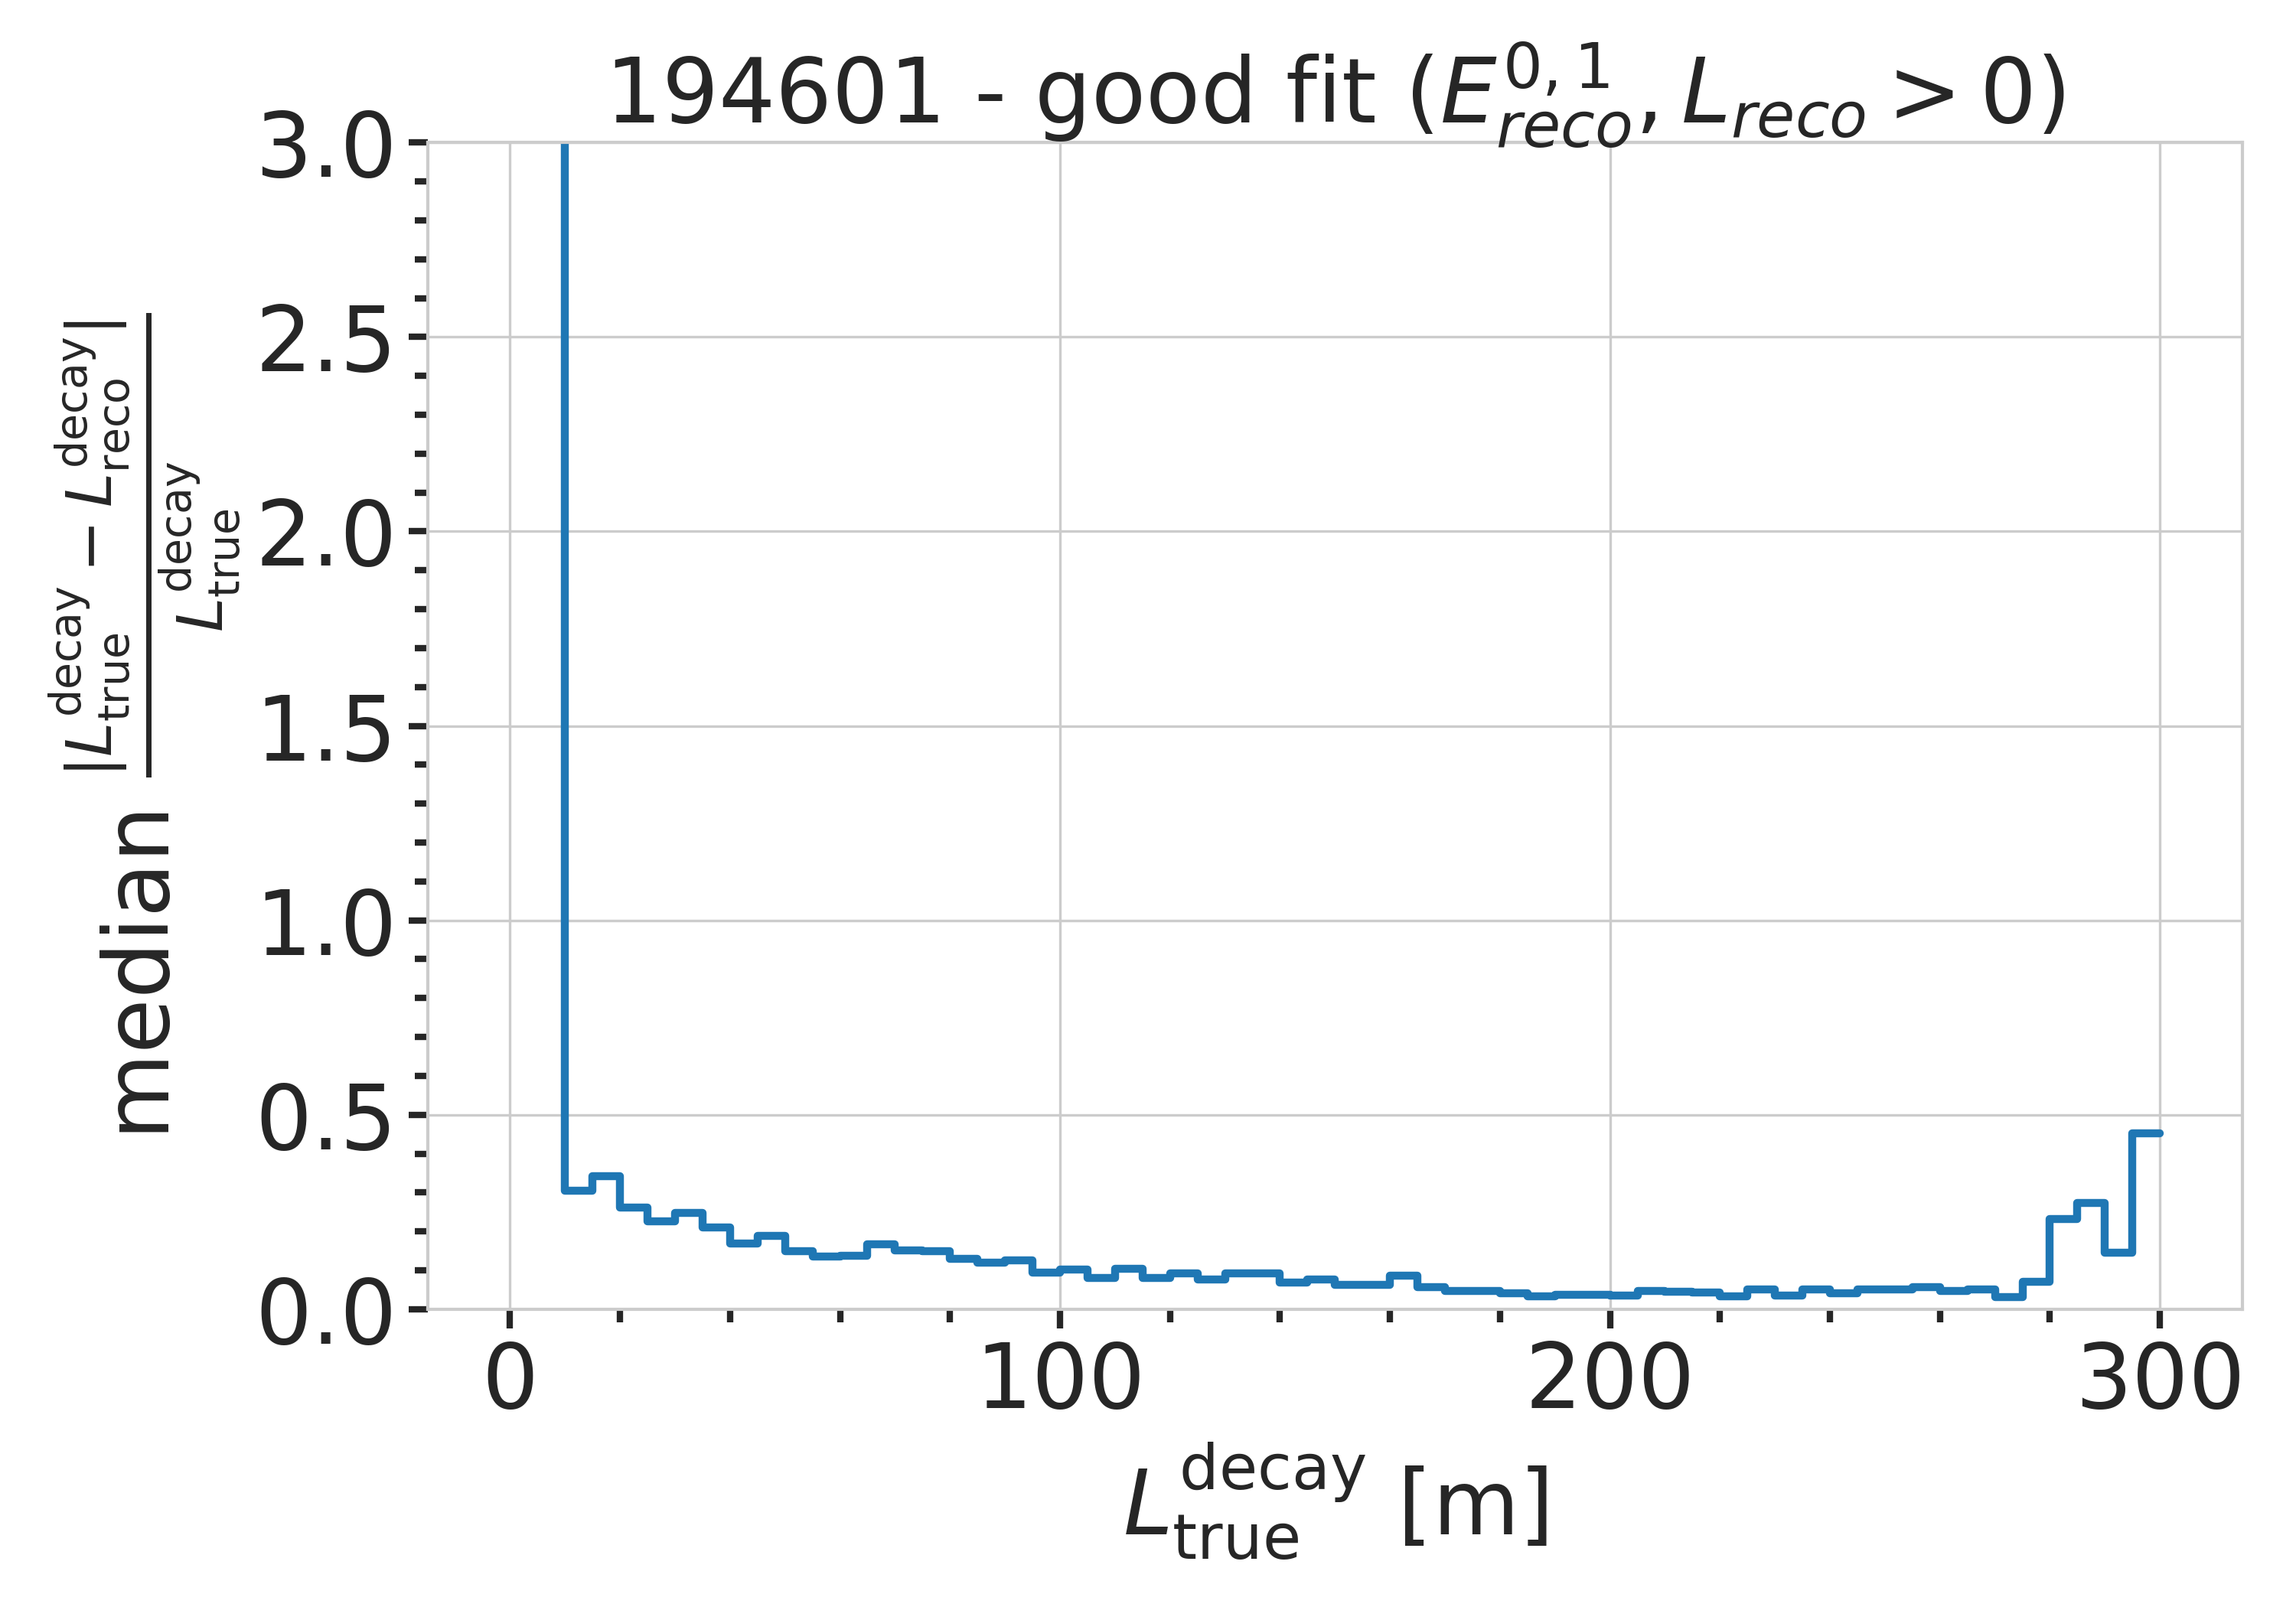
\includegraphics[width=0.47\linewidth]{figures/model_independent_simulation/results/idealistic/194601_median_decay_length_resolution_goodfit_log_unweighted.png}
    \includegraphics[width=0.51\linewidth]{figures/model_independent_simulation/results/idealistic/194601_reco_decay_length_vs_true_decay_length_goodfit_step_contours_new.png}
    \caption[Up-going double-cascade decay length resolution]{Decay length resolution of events from the up-going sample. Shown is the decay length resolution as a function of the true decay length (left) and the reconstructed decay length versus the true decay length (right), where the color scale is normalized per vertical slice and the median and \SI{68}{\percent} band are shown in red.}
    \labfig{idealistic_length_resolutions}
\end{figure*}

The length resolution for events from this sample is shown in \reffig{idealistic_length_resolutions}. In the left part, the median resolution is shown to be below \SI{30}{\percent} above a true decay length of $\sim$\SI{10}{\meter}, and decreasing with increasing true length, down to $\sim$\SI{10}{\percent} at \SI{100}{\meter}. In the right part of \reffig{idealistic_length_resolutions}, the reconstructed decay length versus the true decay length is shown. The color scale shows the PDF along each (vertical) true decay length slice, which additional information highlighted by the median and \SI{68}{\percent} band shown in red (also per vertical column). The two-dimensional histogram shows that there is no under-estimation of the length up to a true decay length of $\sim$\SI{210}{\meter}, which shows that if there are DOMs in the region between the two cascades that have not observed any light, the reconstruction is very stable. Considering the underlying Poisson likelihood in \refeq{millipede_likelihood} used for the reconstruction, this makes sense, since DOMs being present, but not observing any light is affecting the light expectation that goes into the likelihood and therefore makes these hypotheses incompatible with the data.


\subsubsection{Realistic Events}

The sample of HNL events introduced in \refsec{realistic_sample}, which is a more realistic representation of the expected HNL events, but still offers more controlled energy and length distributions, is used to investigate the selection efficiency, to cross-check the reconstruction performance, and to benchmark the limits where the reconstruction breaks down. An example event view is shown in \reffig{realistic_example_event}, for cascade energies of \SI{30.8}{\gev} and \SI{25.3}{\gev}, and a decay length of \SI{144.5}{\meter}. Since the size of the colored spheres is proportional to the number of photons observed in the DOMs, it can be seen from the event view that even for these higher energies, only individual or few photons are observed. This makes detecting and reconstructing them significantly more challenging and is purely due to the larger distance of the cascades from the DOMs.

\begin{marginfigure}
    \centering
    % [trim=left bottom right top, clip]
    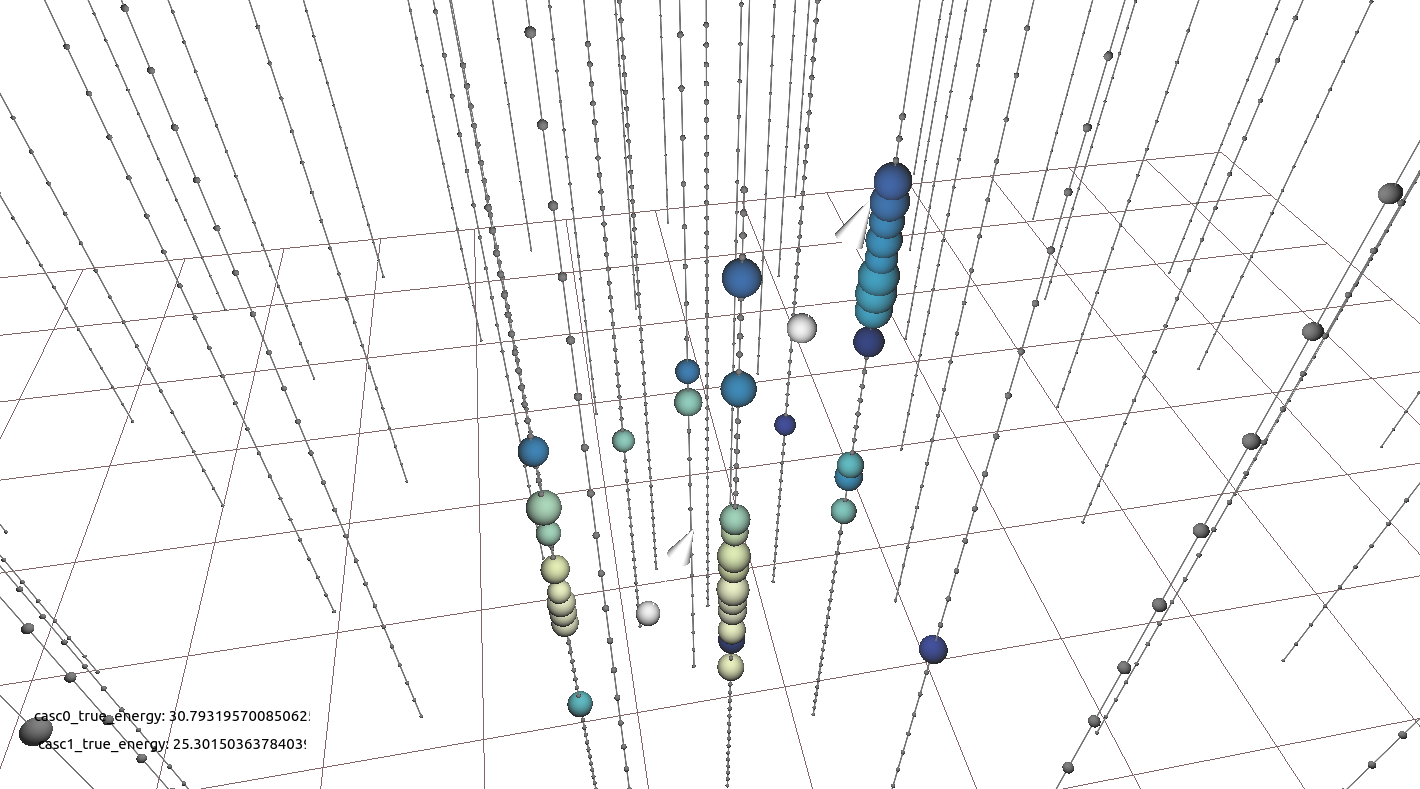
\includegraphics[trim=230 45 230 65, clip]{figures/model_independent_simulation/diagonal_e0_30.8_e1_25.3_v0.png}
    \caption[Event view of a realistic double-cascade event]{Event view of a realistic double-cascade event, with cascade energies of \SI{30.8}{\gev} and \SI{25.3}{\gev}, and a decay length of \SI{144.5}{\meter}. The colored spheres show the DOMs that have observed light, where the size is proportional to the number of observed photons and the color indicates the time (yellow is early, blue is late). The strings are shown as black lines, with small spheres indicating the DOM positions, and the true cascade vertices and directions are shown as white spheres with white arrows.}
    \labfig{realistic_example_event}
\end{marginfigure}


\paragraph{Energy Resolutions:}

The energy resolutions are inspected by looking at the two-dimensional distributions of reconstructed energy versus the true energy. The results for the energies of the individual cascades are shown in \reffig{cascade_energy_2dhists}, where the color scale is again normalized per vertical slice, and the median and \SI{68}{\percent} band are shown in red. For both cascades the reconstruction performs well above around \SIrange{5}{7}{\gev}, with the median being on top of the diagonal and the spread being small. Below this energy, the reconstruction is over-estimating the true energy. This is because, on average, those low-energy events, passing the event selection, interact closer to the DOMs and have an over fluctuation in their light deposition. This results in the observed energy bias. Interestingly, the second cascade energy reconstruction performs slightly worse, although they have the same energy ranges for this sample. This could hint at an asymmetry in the reconstruction process, which might be related to how the two cascades are parameterized, or be due to the different positions and the dominantly up-going direction used in the sampling combined with the DOMs looking down. Towards the higher energies, the statistics are decreasing, wich is due to the underlying energy distribution of the sample, which were shown in \reffig{realistic_gen_distris}.


\begin{figure*}[h]
    \centering
    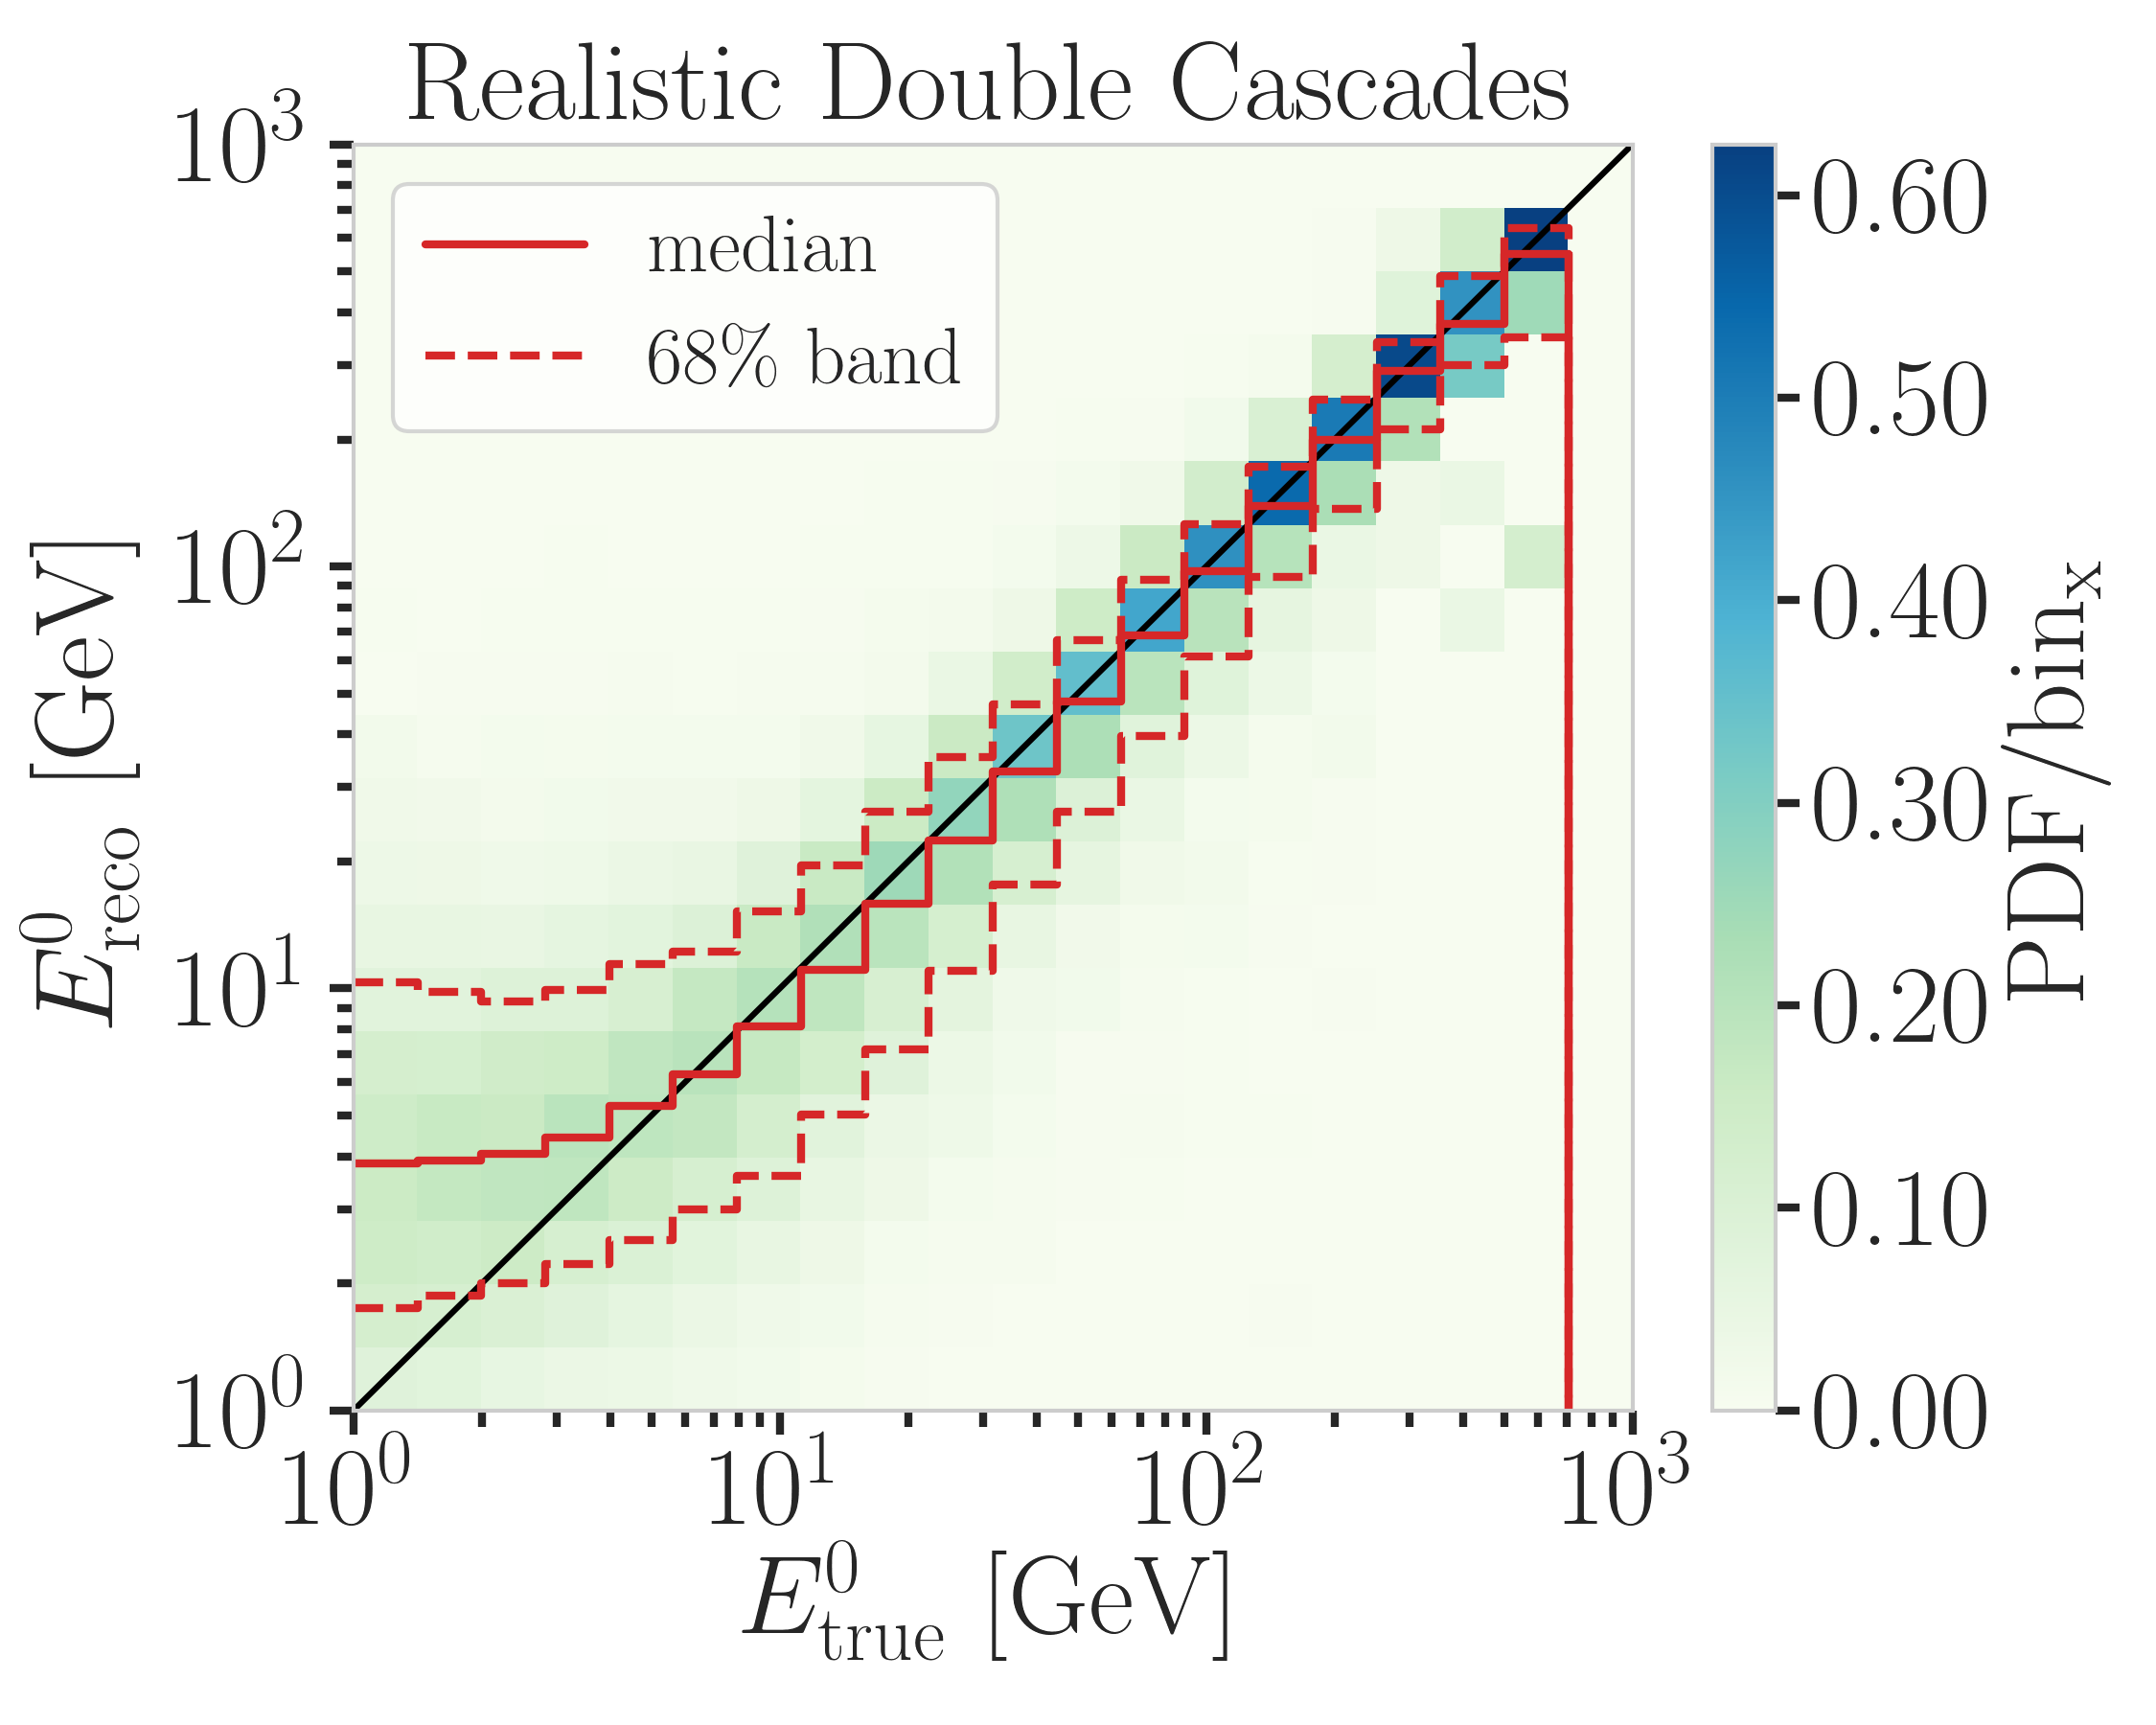
\includegraphics[width=0.49\linewidth]{figures/model_independent_simulation/results/realistic/2d_hists/194603_casc0_reco_energy_vs_casc0_true_energy_goodfit_step_contours.png}
    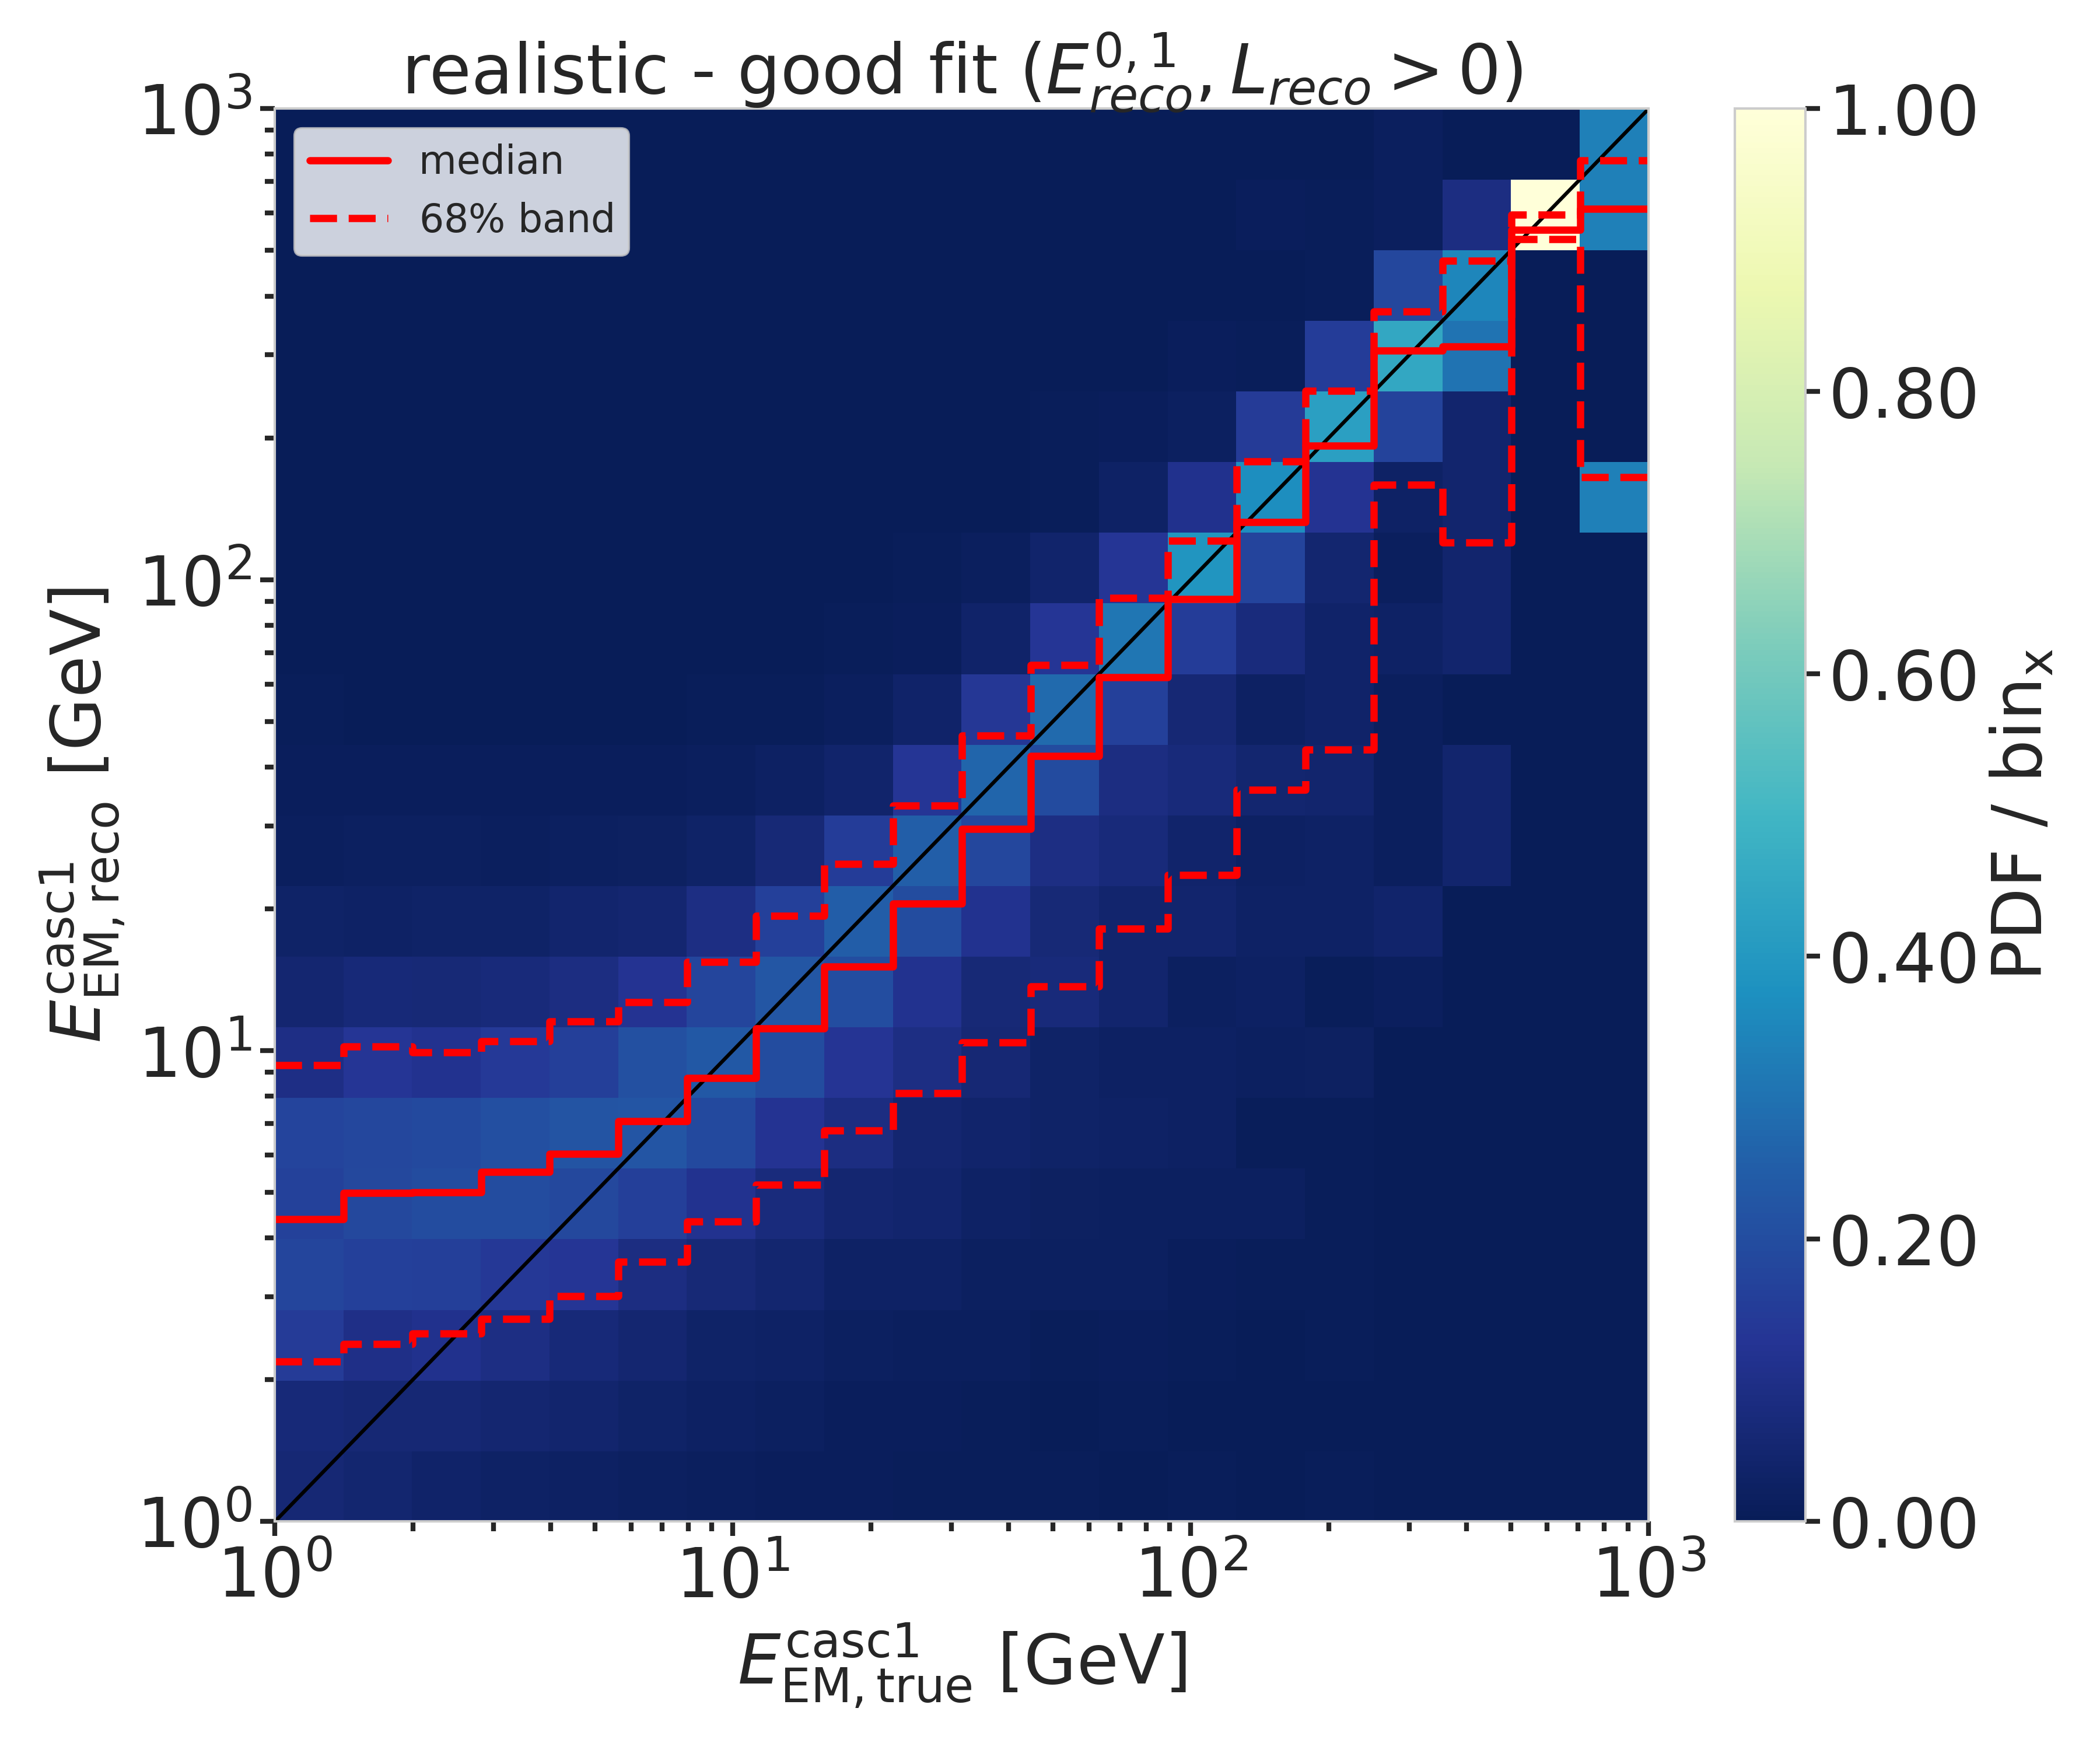
\includegraphics[width=0.49\linewidth]{figures/model_independent_simulation/results/realistic/2d_hists/194603_casc1_reco_energy_vs_casc1_true_energy_goodfit_step_contours.png}
    \caption[Realistic double-cascade energy resolutions]{Energy resolutions of the realistic, model-independent simulation sample. Shown is the reconstructed energy versus the true energy for both cascades, where the color scale is normalized per vertical slice and the median and \SI{68}{\percent} band are shown in red.}
    \labfig{cascade_energy_2dhists}
\end{figure*}


\paragraph{Decay Length Resolutions:}

The reconstructed decay length versus the true decay length is shown for all events in the left part of \reffig{realistic_sample_decay_length_2dhists}. For short true decay lengths the reconstruction is over-estimating the length, while for long true decay lengths the reconstruction is strongly under-estimating the length. There is a region between true decay lengths of \SIrange[range-phrase=~and~]{15}{80}{\meter} where the median reconstruction is almost unbiased, but the \SI{68}{\percent} interquartile range is wide with a lot of outliers towards short reconstructed lengths. Below \SI{15}{\meter} the reconstructed lengths are always over-estimating the true length and above \SI{80}{\meter} a population of events with short reconstructed length starts to dominate.

The over-estimation at small true decay lengths can be explained by multiple factors, one being that the shortest DOM spacing is $\sim$\SI{7}{\meter}, vertically for DeepCore strings, but mostly larger than that, so resolving lengths below that is very challenging. The reconstruction tends to be biased towards estimating the length around where the light was observed. Additionally, approaching a length of 0.0, the reconstructed length will of course always be a one-sided distribution, because the lengths have to be positive.

\begin{figure*}[h]
	\centering
    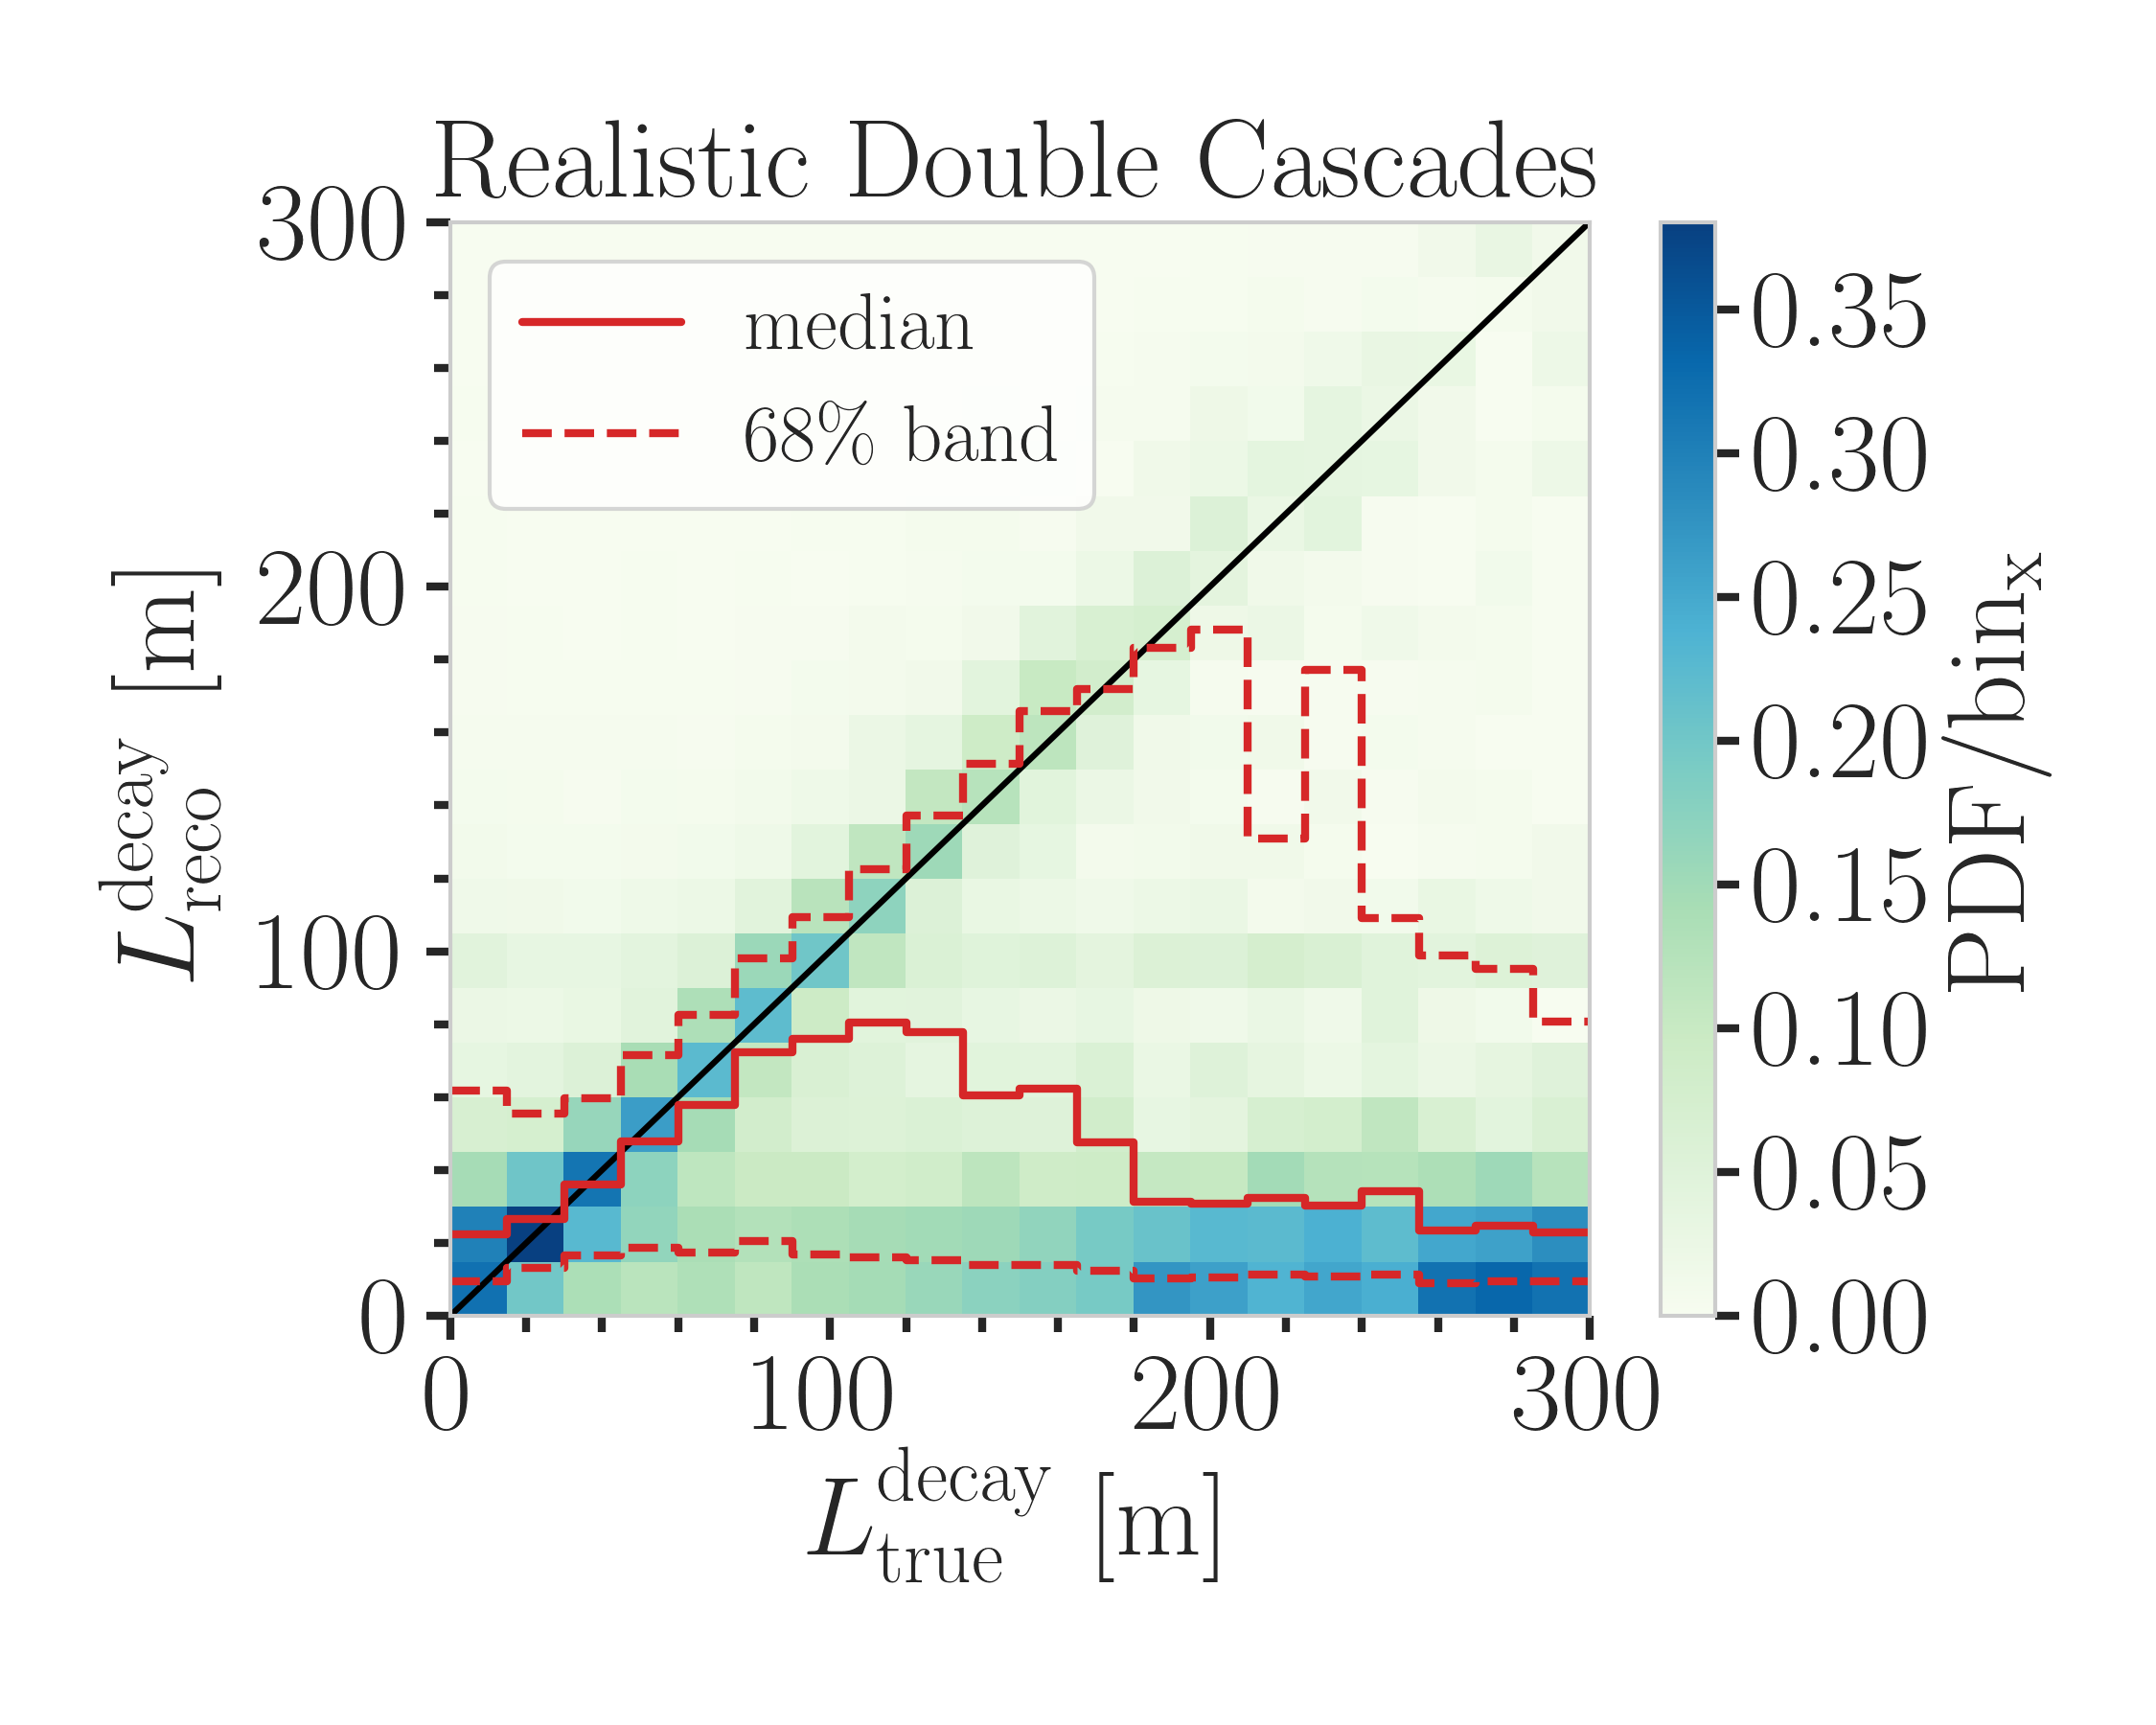
\includegraphics[width=0.49\linewidth]{figures/model_independent_simulation/results/realistic/2d_hists/194603_reco_decay_length_vs_true_decay_length_goodfit_step_contours.png}
    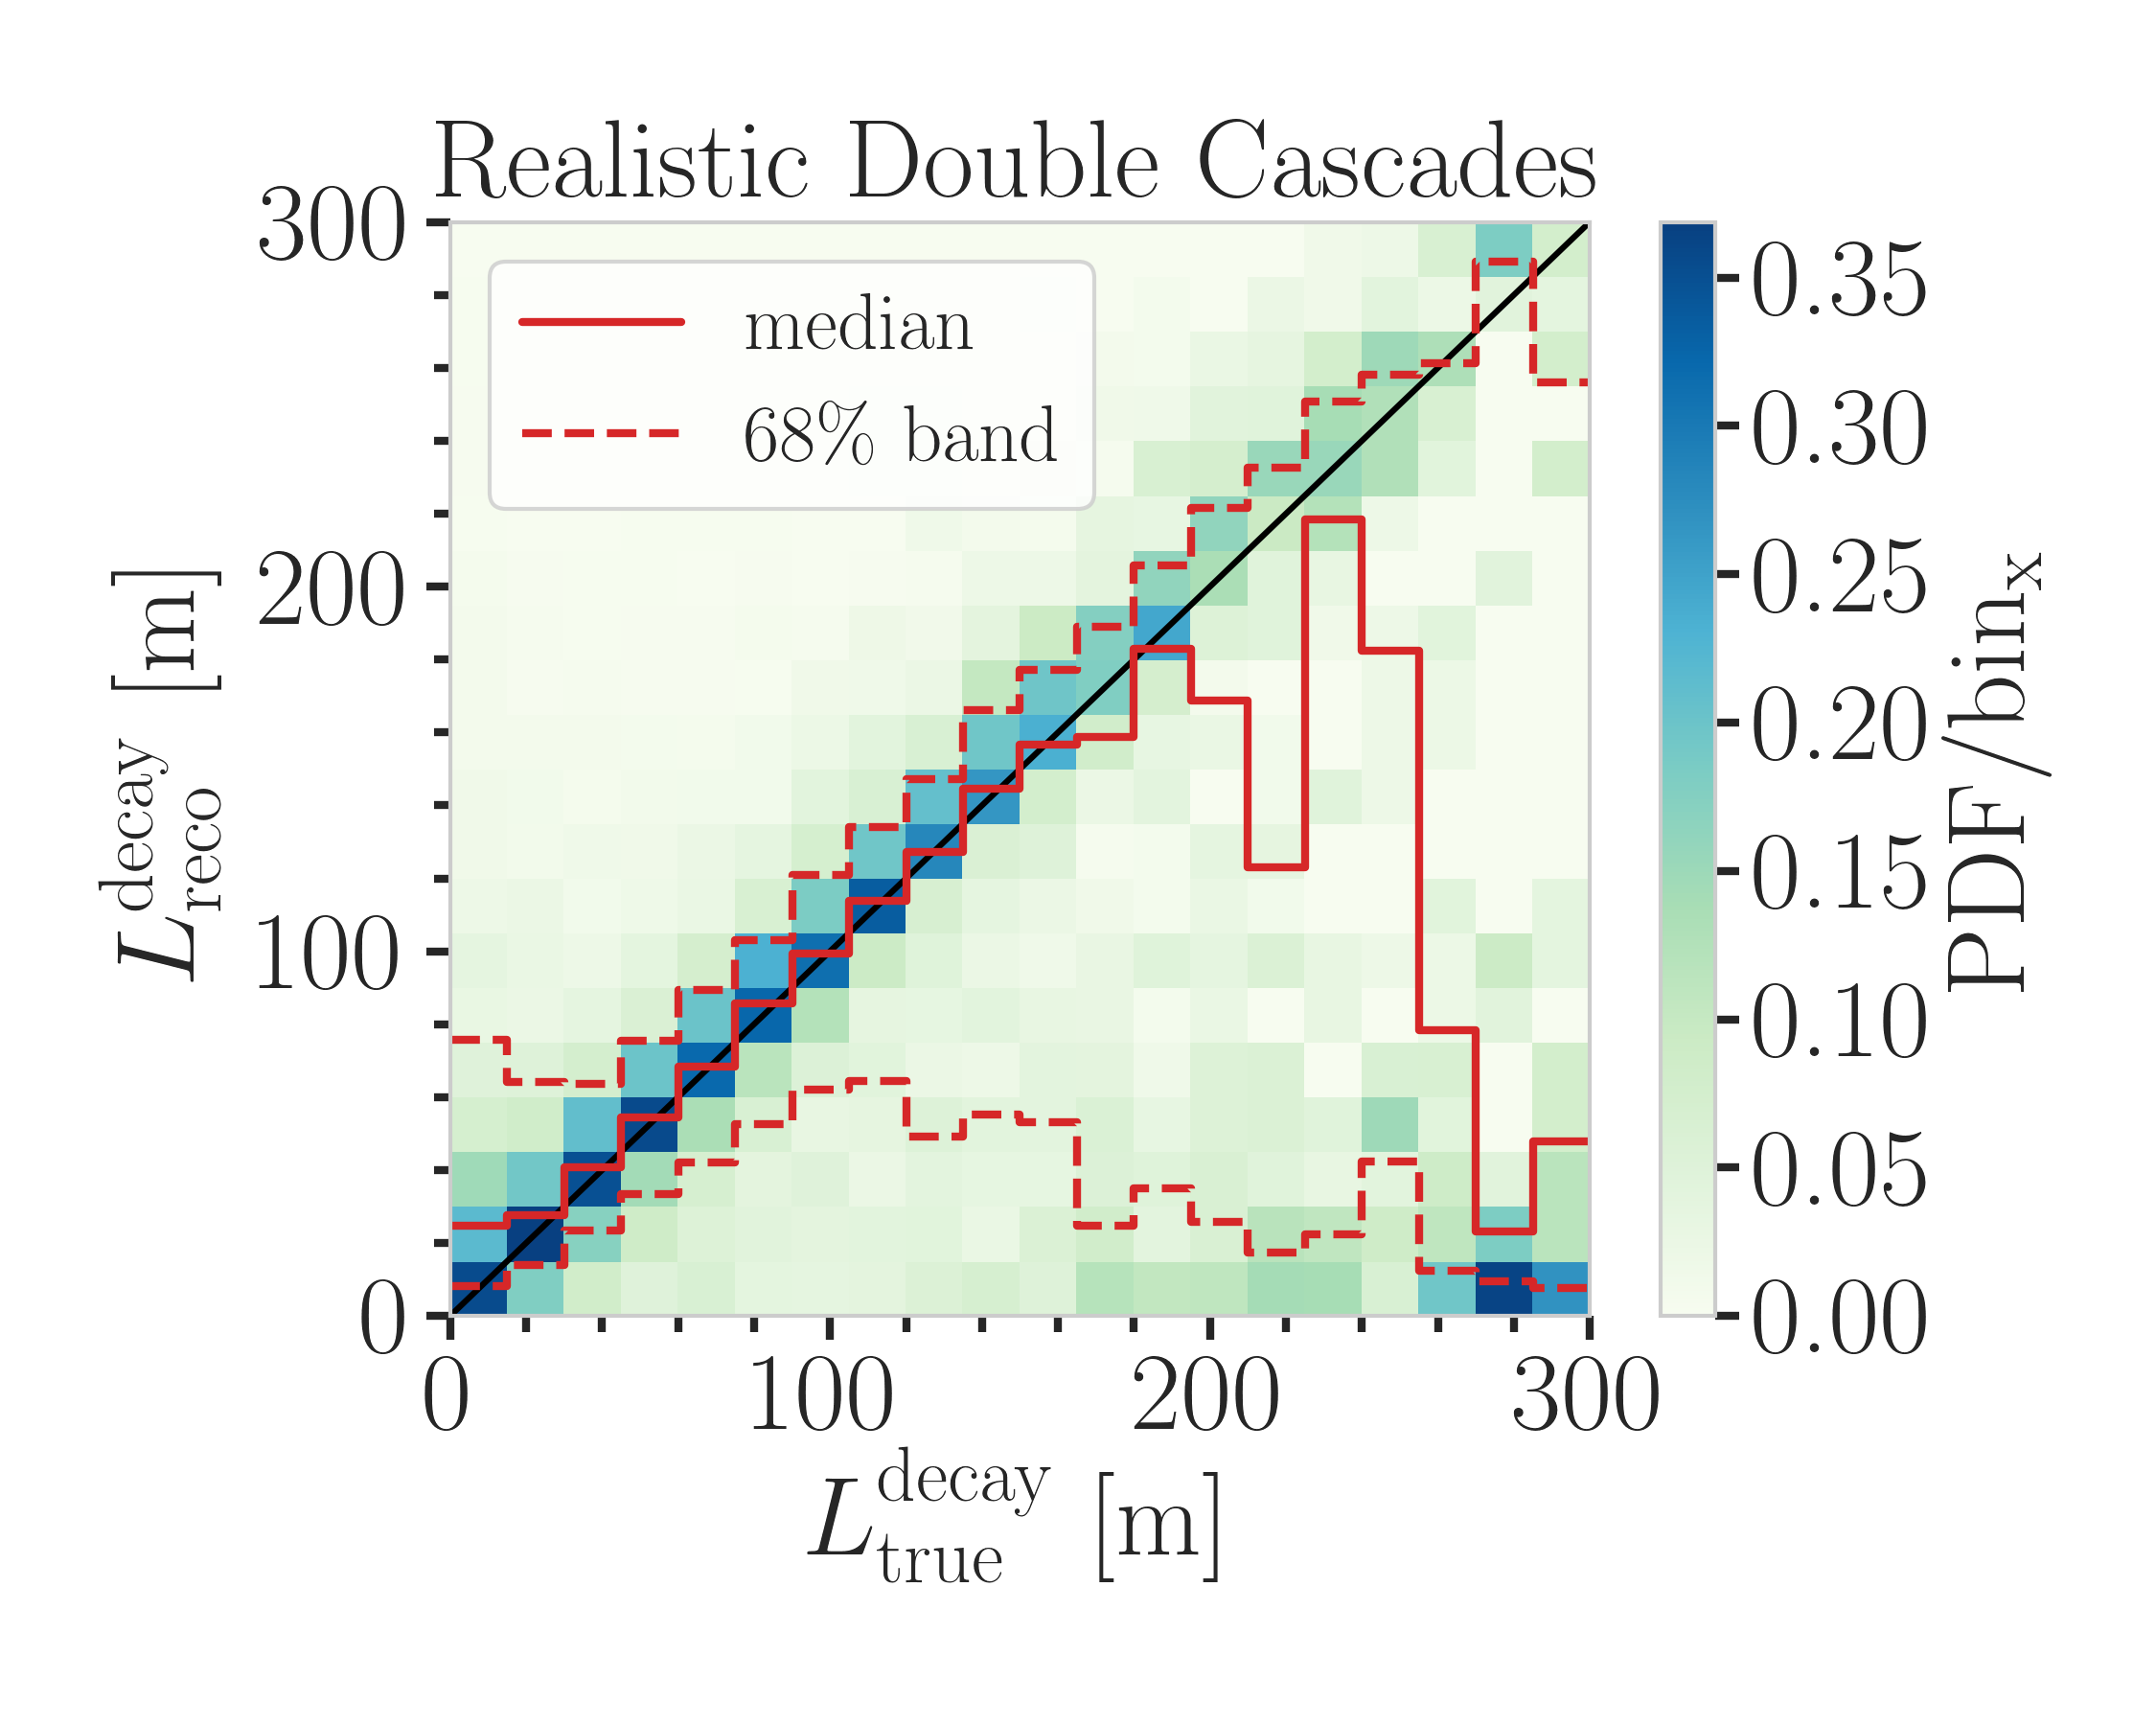
\includegraphics[width=0.49\linewidth]{figures/model_independent_simulation/results/realistic/2d_hists/194603_reco_decay_length_vs_true_decay_length_goodfit_above_10_GeV_step_contours}
    \caption[Realistic double-cascade length resolution]{Length resolution of the realistic, model-independent simulation sample. Shown is the two-dimensional histograms of the reconstructed length versus the true length for all events (left) and for events with reconstructed cascade energies larger than \SI{10}{\gev} (right), where the color scale is normalized per vertical slice and the median and \SI{68}{\percent} band are shown in red.}
    \labfig{realistic_sample_decay_length_2dhists}
\end{figure*}

The under-estimation at large true decay lengths is more puzzling. It seems like the distribution becomes bimodal in the reconstructed lengths. There is one well reconstructed population around the diagonal, and another badly reconstructed population at very short reconstructed lengths. Above \SI{150}{\meter} the badly reconstructed population starts to dominate, and the median resolution drops off strongly. For these events, only one cascade was observed with enough light to be reconstructed, and the reconstruction describes the one observed cascade in two parts, separated by a short distance. The result of applying a minimum energy cut on the reconstructed cascade energies ($E^0, E^1 \ge \SI{10}{\gev}$) is shown in the right part of \reffig{realistic_sample_decay_length_2dhists}. It can be seen that the median resolution improves significantly, now aligning with the expectation between \SIrange[range-phrase=~and~]{15}{160}{\meter}. The spread also improves, but is still biased towards short reconstructed lengths and above \SI{200}{\meter} the badly reconstructed population starts to dominate again.


\paragraph{Resolution Benchmarks:}

\begin{figure*}[h]
	\centering
    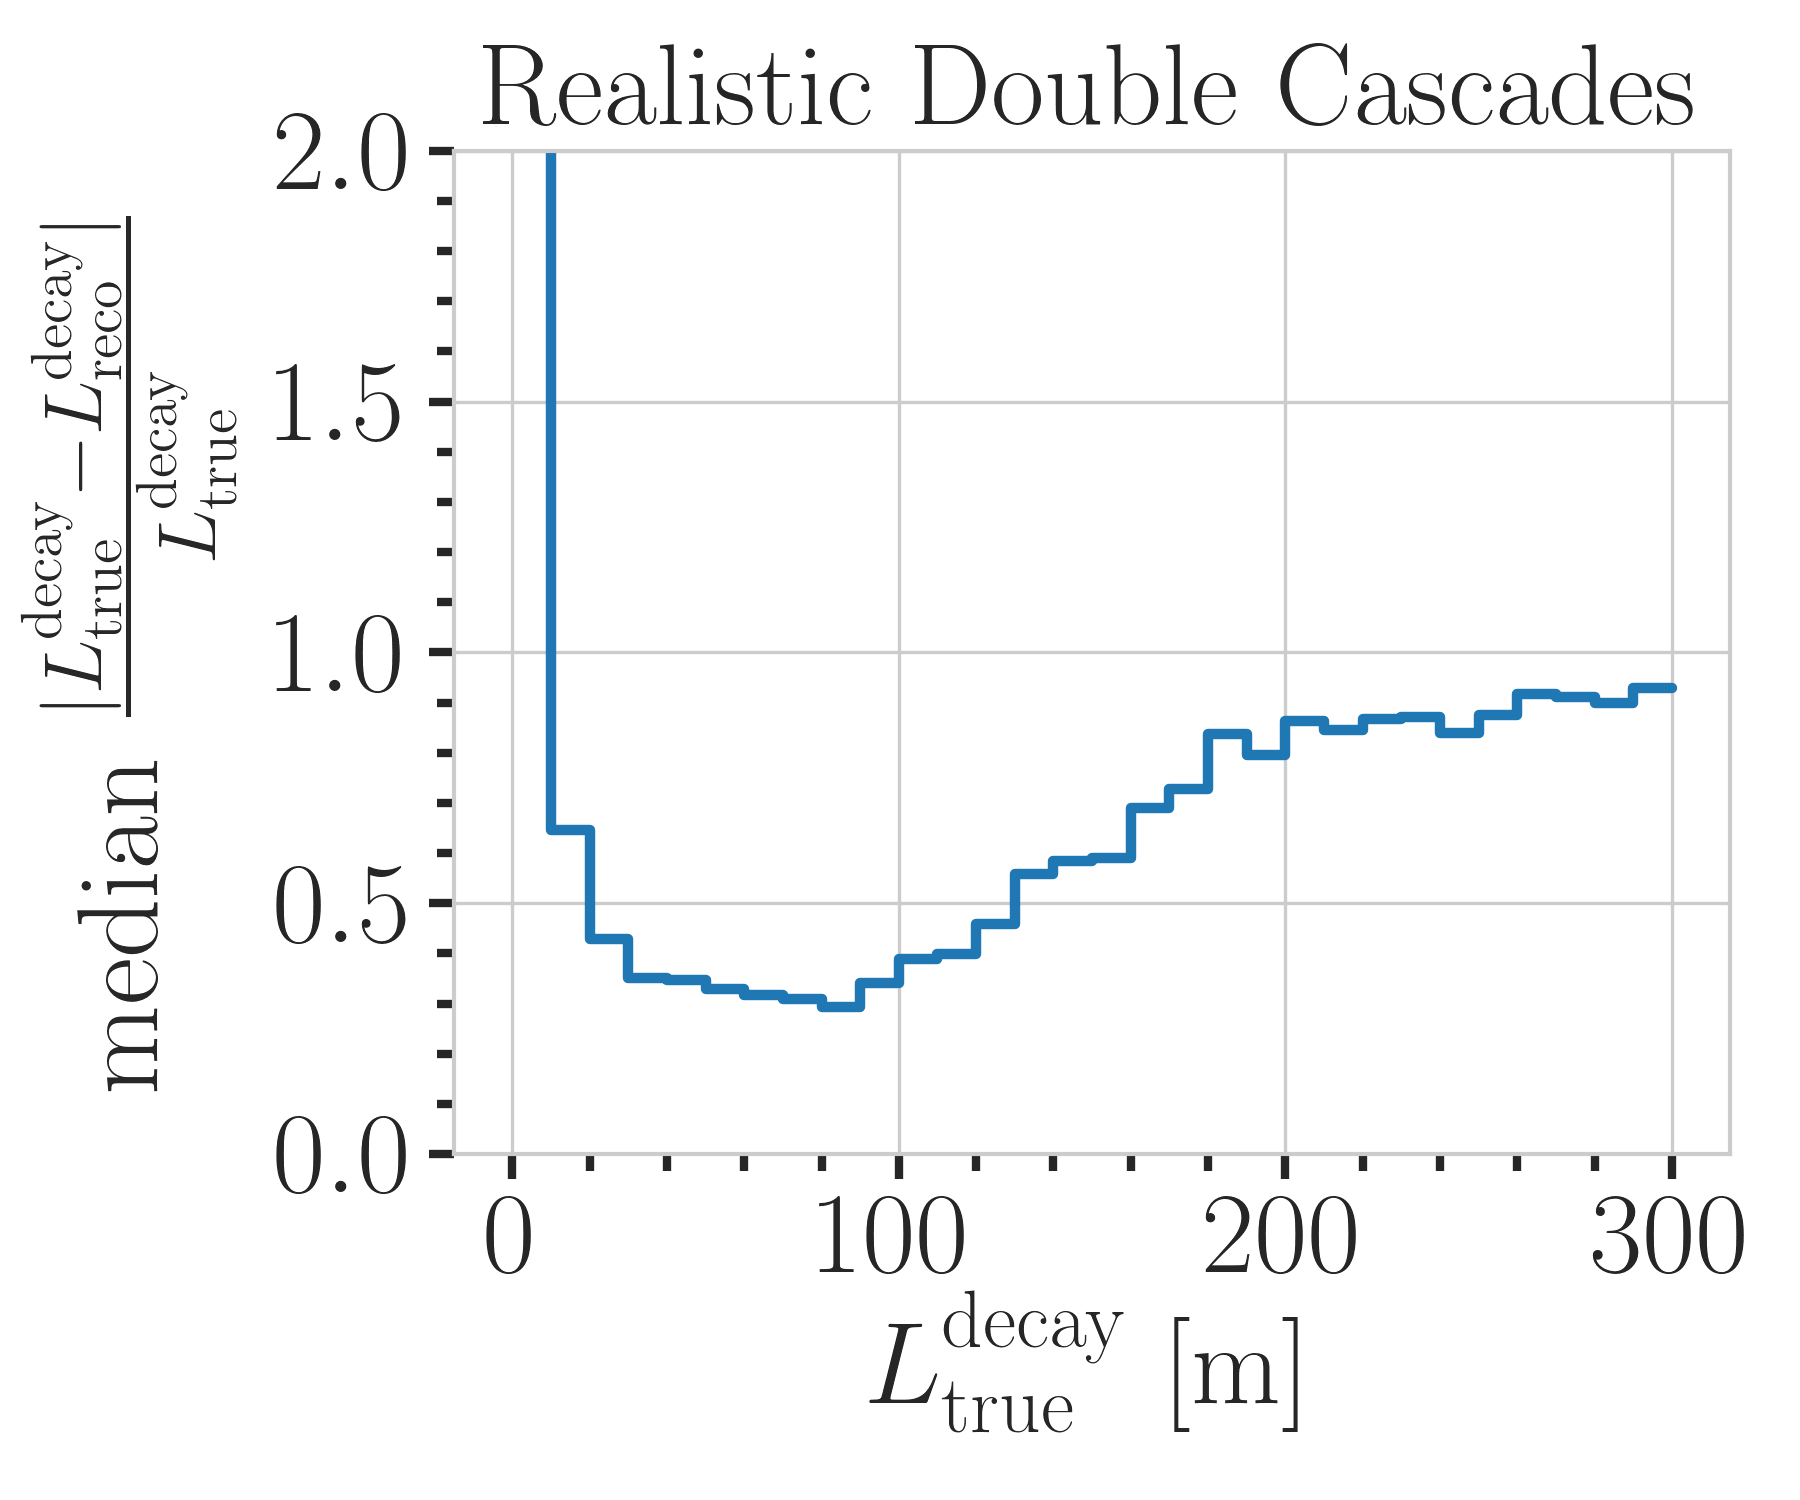
\includegraphics[width=0.45\linewidth]{figures/model_independent_simulation/results/realistic/resolutions/194603_median_decay_length_resolution_goodfit_log_unweighted.png}
    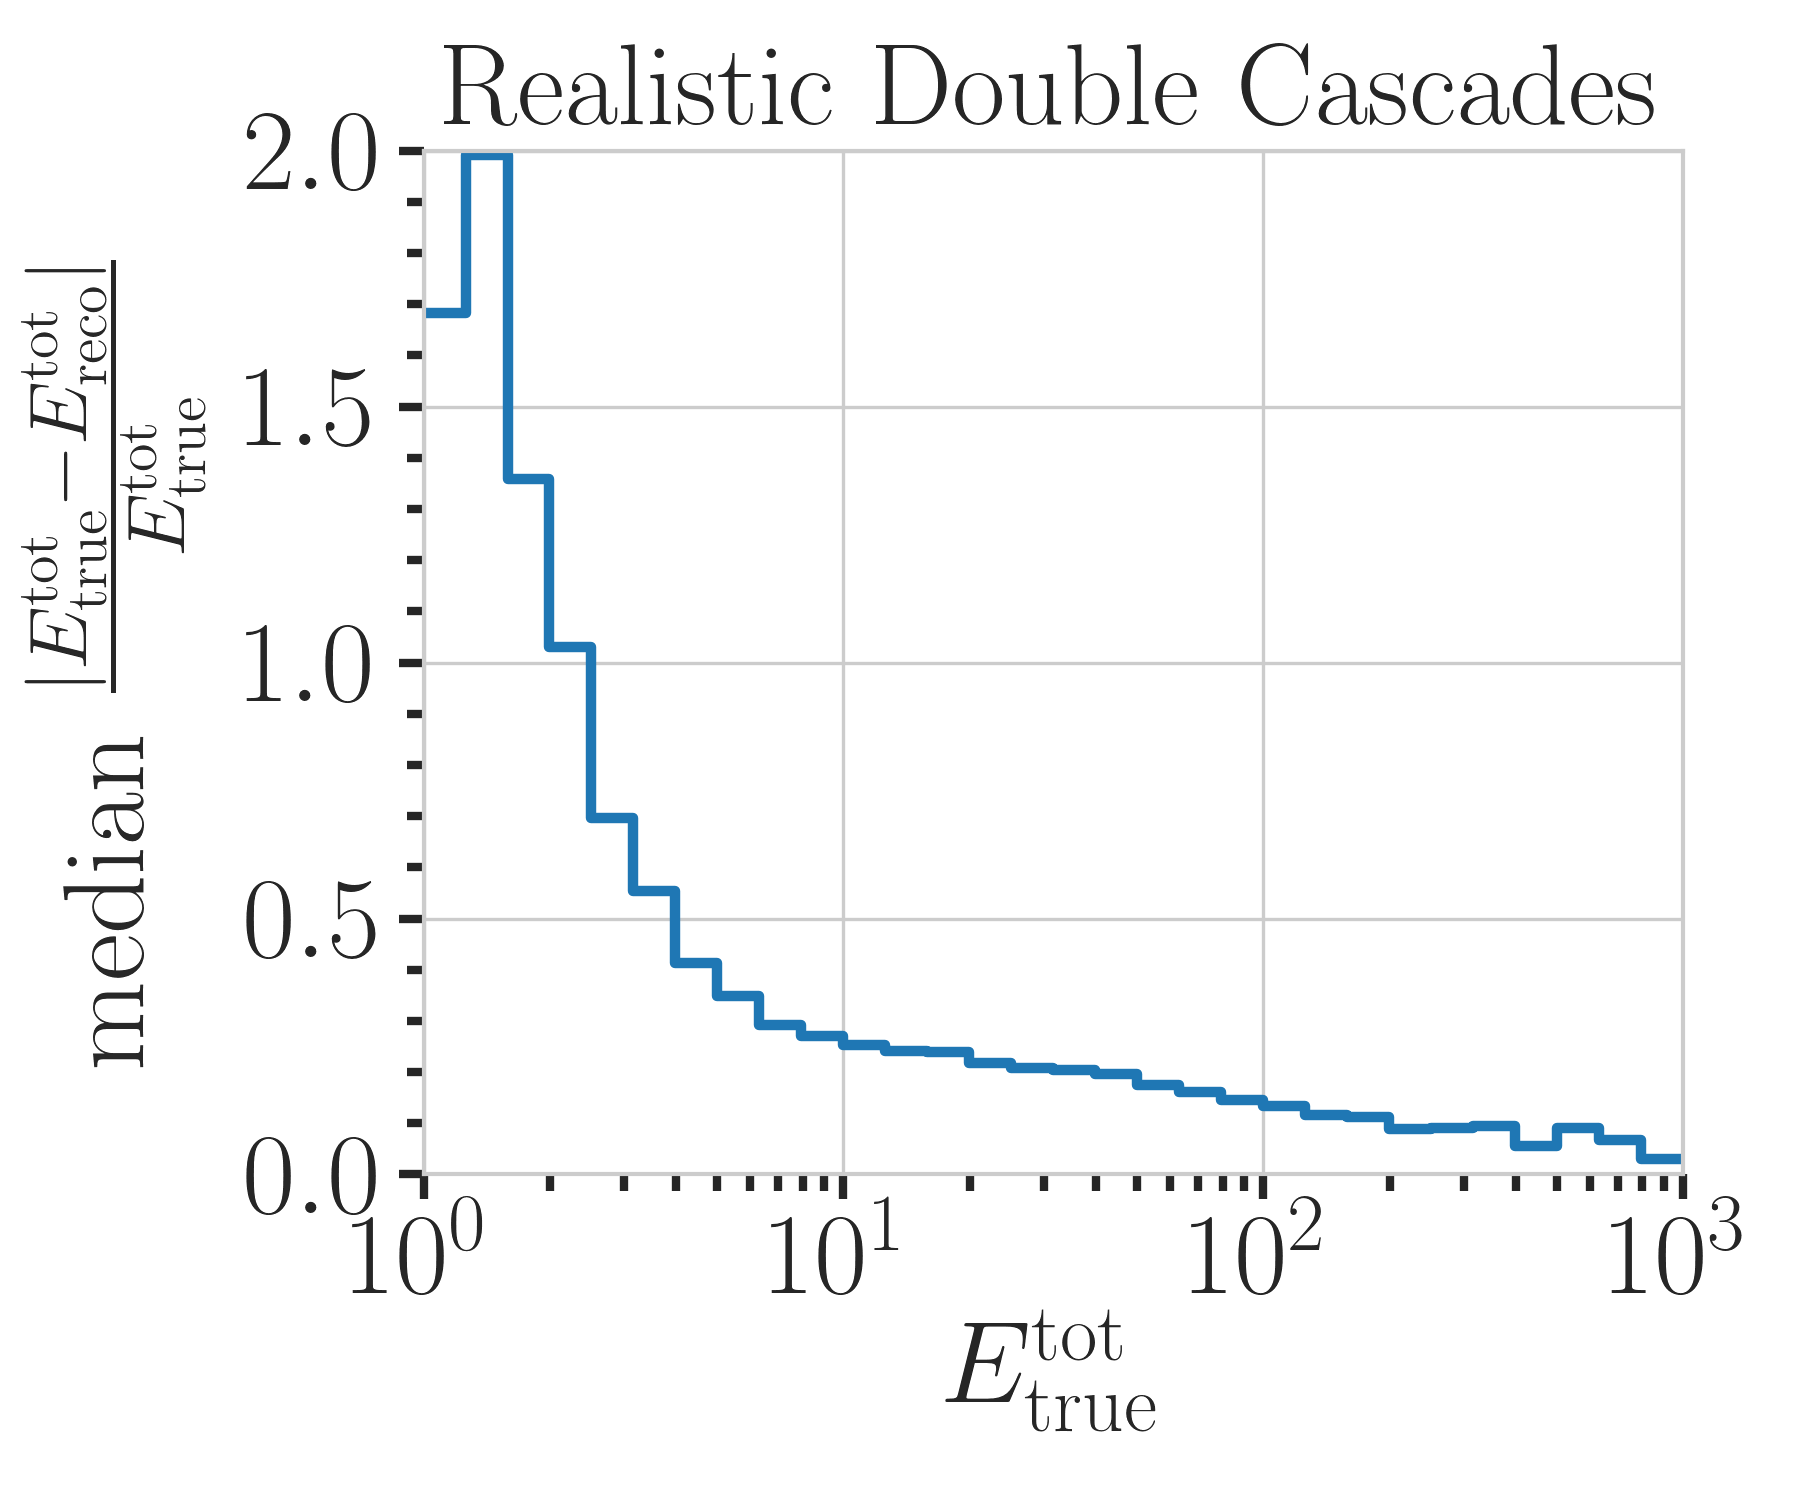
\includegraphics[width=0.45\linewidth]{figures/model_independent_simulation/results/realistic/resolutions/194603_median_absolute_fractional_reco_total_energy_error_goodfit.png} 
    \caption[Realistic double-cascade decay length and total energy resolution]{Decay length and total energy resolution of events from the realistic sample. Shown is the decay length resolution as a function of the true decay length (left) and the total energy resolution as a function of the true total energy (right).}
    \labfig{median_resolutions_energy_length}
\end{figure*}

The left part of \reffig{median_resolutions_energy_length} shows the median resolutions of the decay length as a function of the true decay length. It falls below \SI{65}{\percent} above a true decay length of $\sim$\SI{10}{\meter}, and starts to increase again with increasing true length around \SI{100}{\meter}, where it is at \SI{40}{\percent}. For larger true decay length, where the badly reconstructed population dominates, the resolution is large, stabilizing at around \SI{90}{\percent} at \SI{200}{\meter}. This is a significantly worse behavior than the performance found for the best-case event types shown in the left part of \reffig{idealistic_length_resolutions}. The total energy resolution versus the true total energy is shown in the right part of \reffig{median_resolutions_energy_length}. Above \SI{4}{\gev} it is good and constantly improving with the true total energy. It falls below \SI{30}{\percent} at \SI{10}{\gev} and reaches \SI{15}{\percent} at \SI{100}{\gev}.

\begin{figure*}[h]
	\centering
    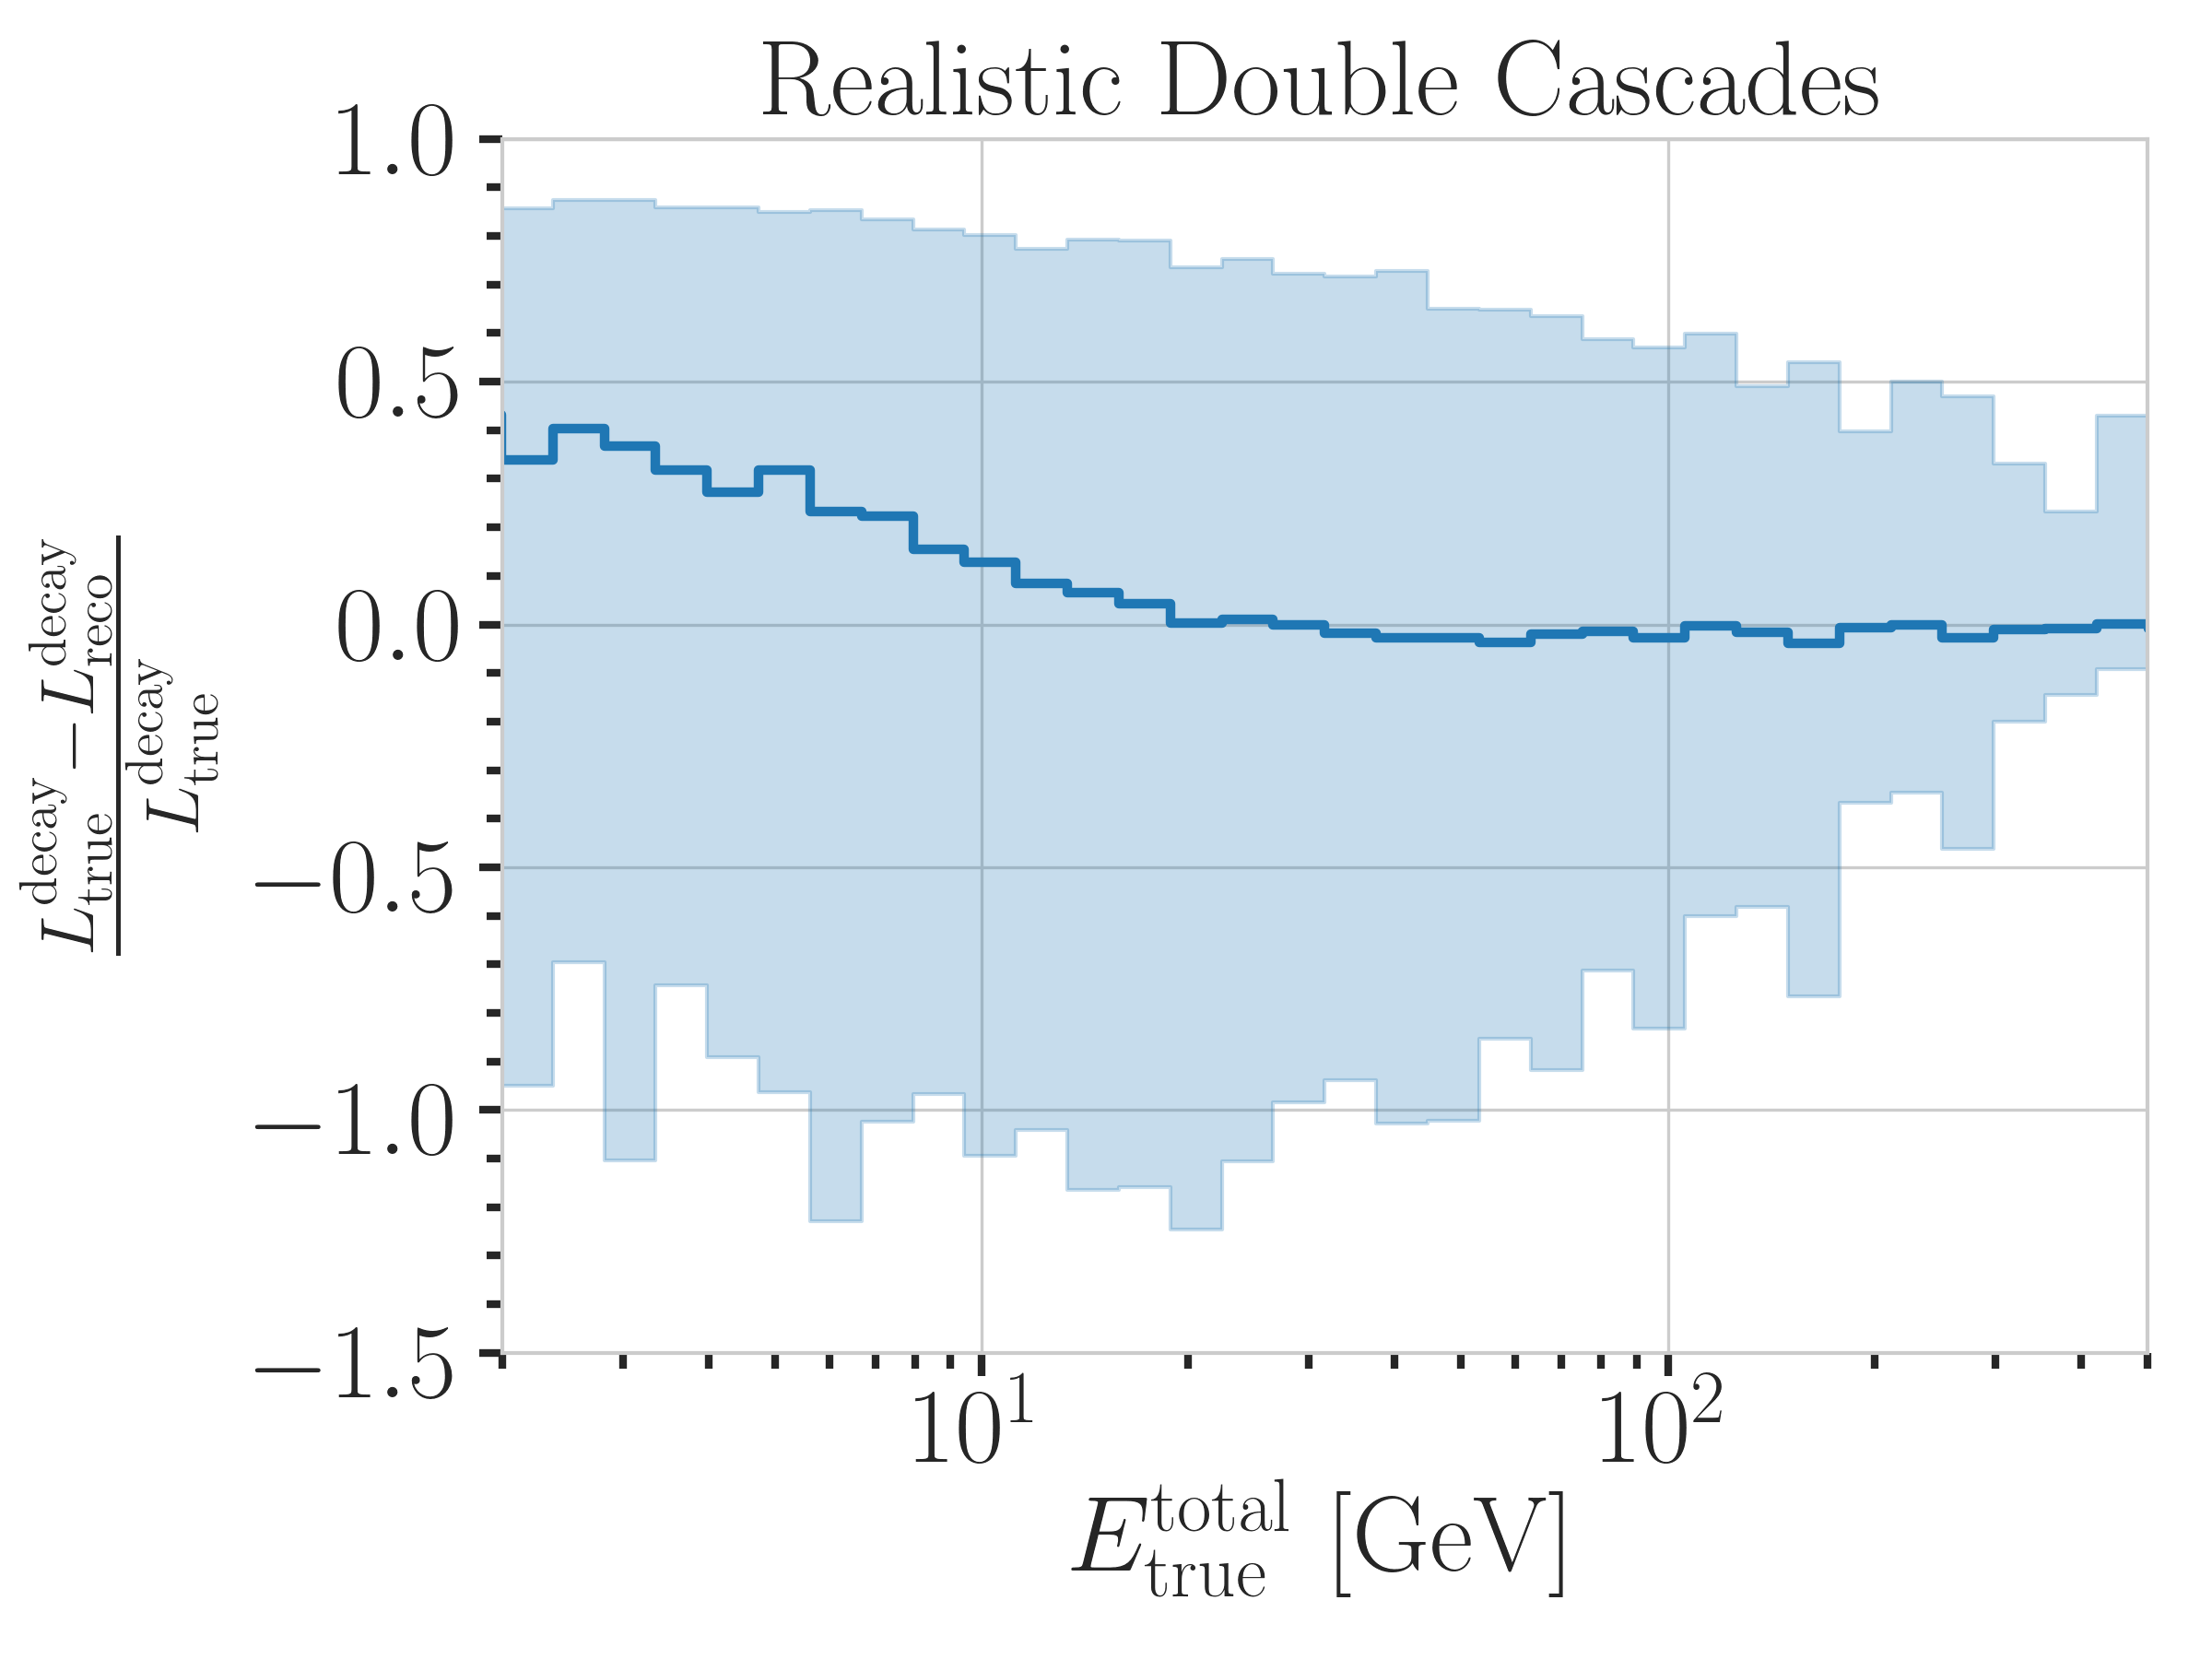
\includegraphics[width=0.49\linewidth]{figures/model_independent_simulation/results/realistic/resolutions/194603_median_decay_length_bias_vs_tot_energy_goodfit_log_unweighted.png}
    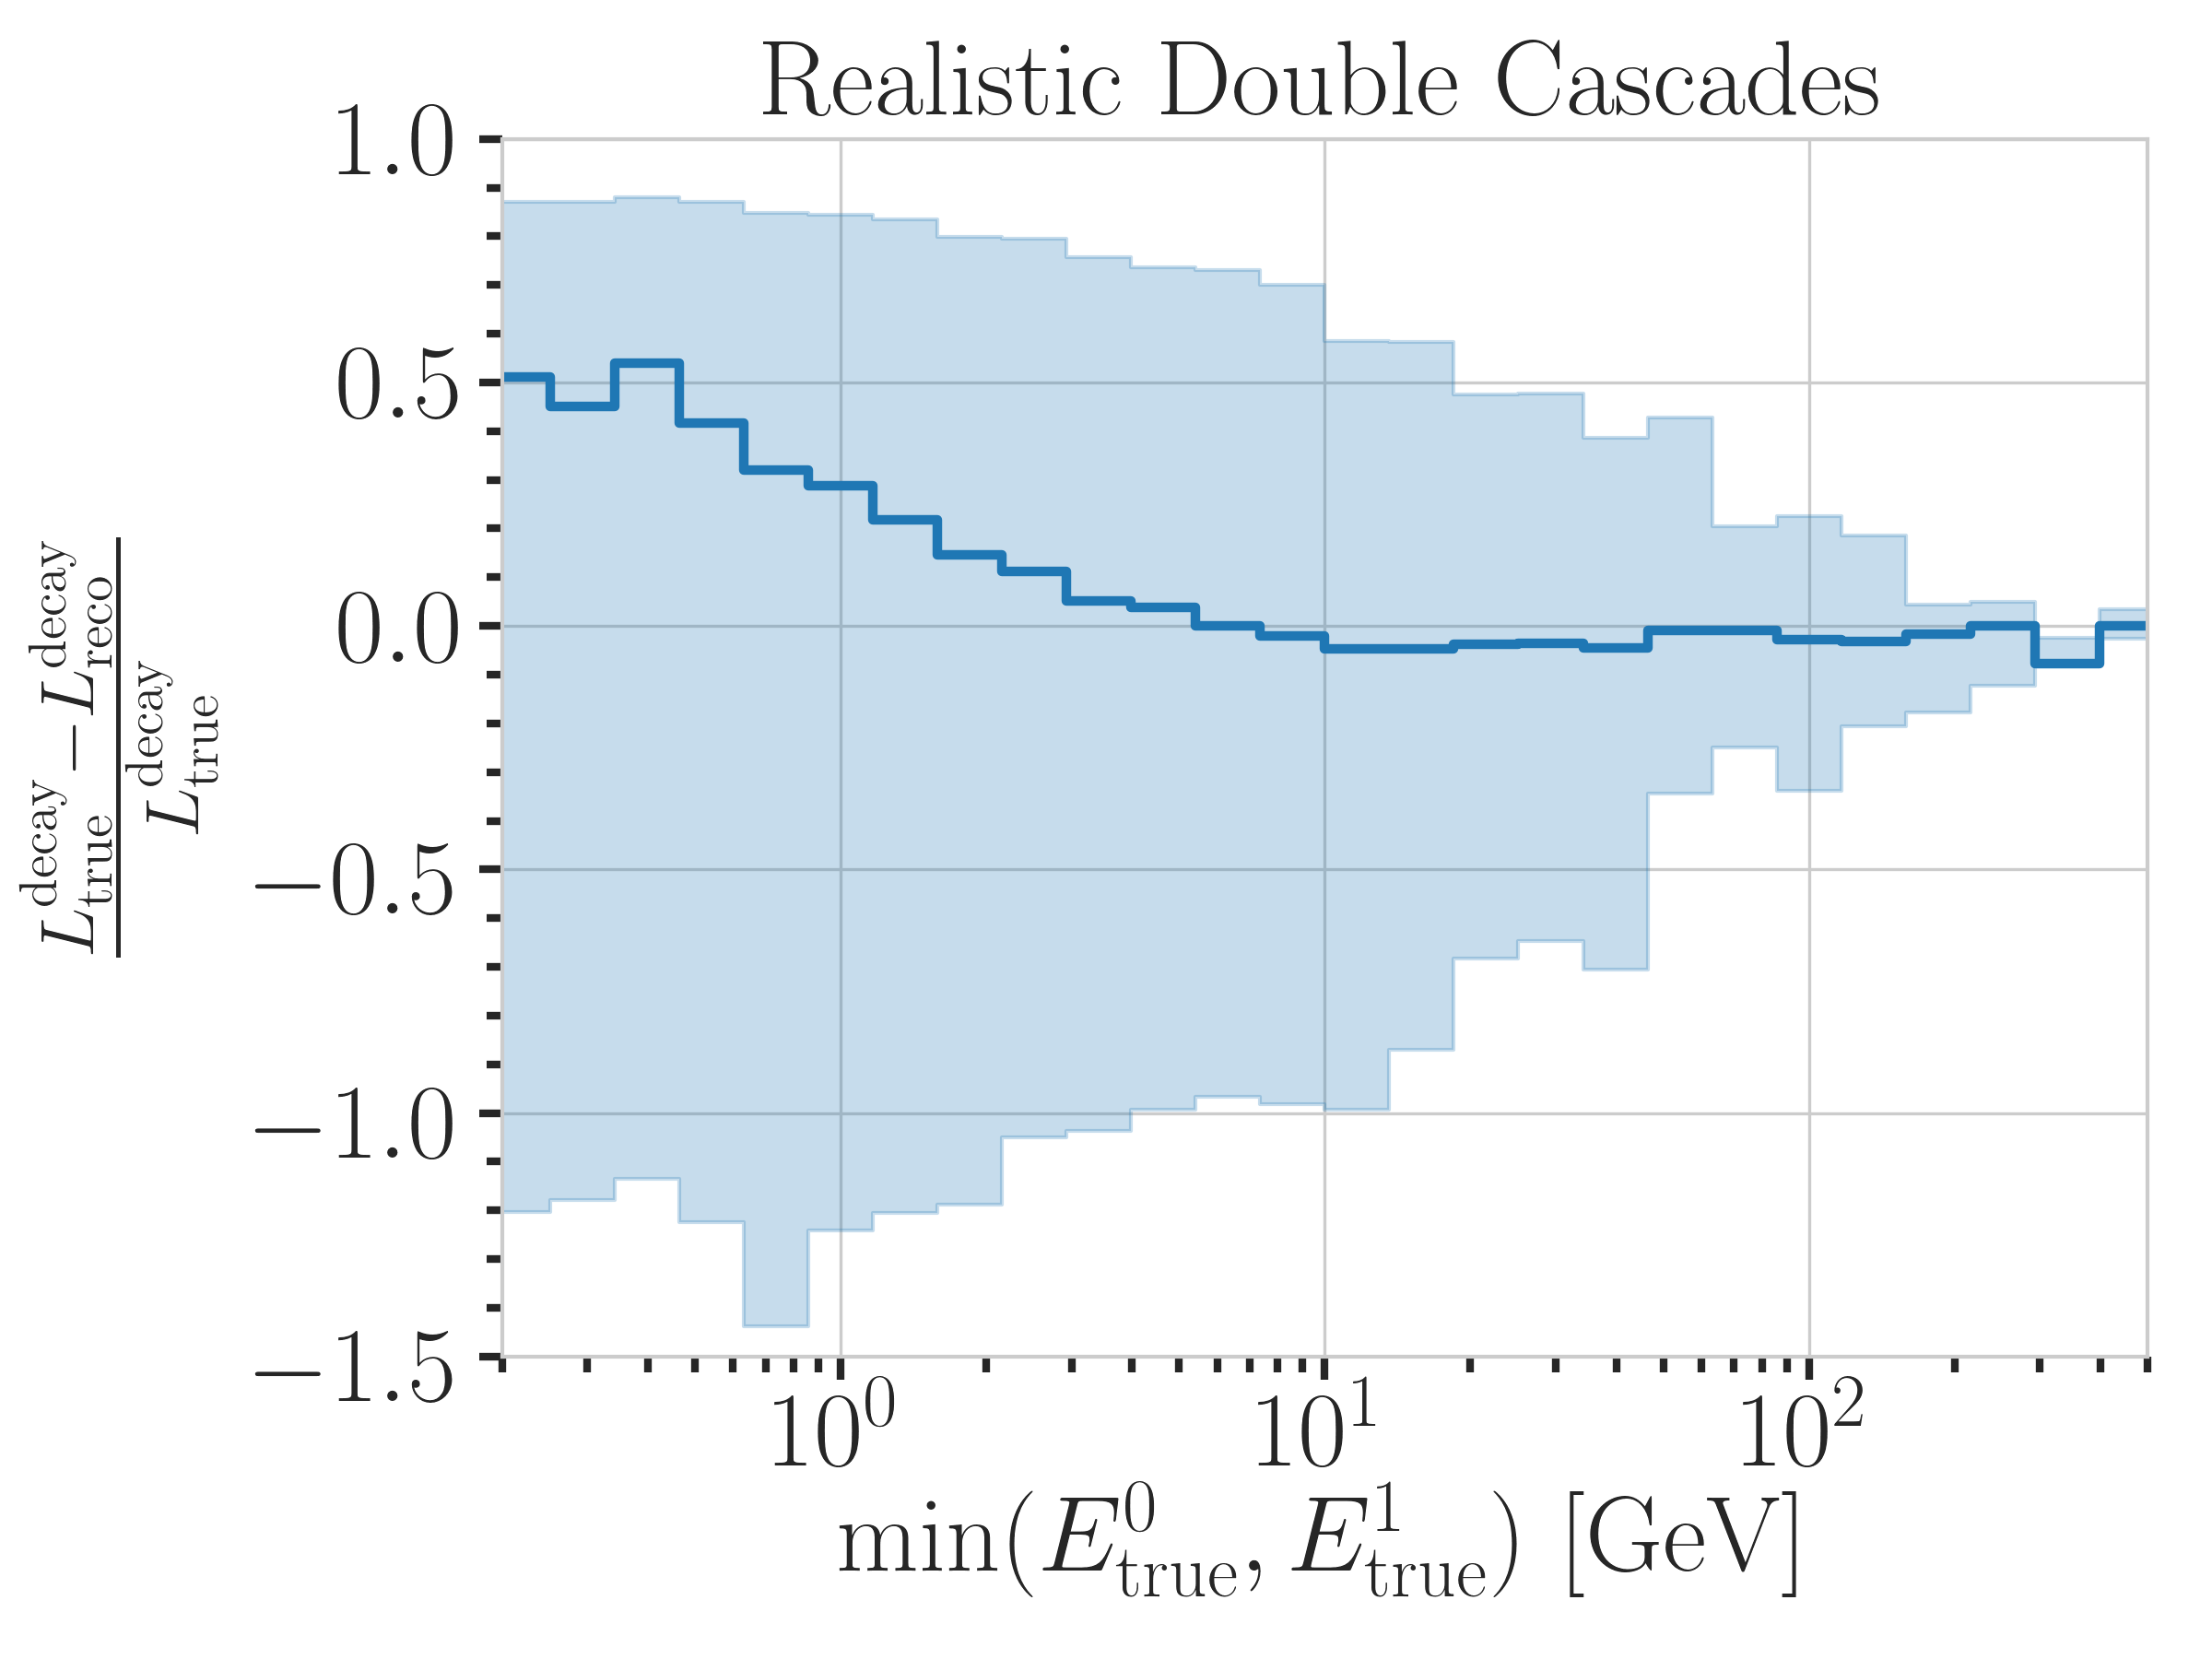
\includegraphics[width=0.49\linewidth]{figures/model_independent_simulation/results/realistic/resolutions/194603_median_decay_length_bias_vs_min_energy_goodfit_log_unweighted.png} 
    \caption[Realistic double-cascade decay length resolution versus energies]{Decay length resolution of events from the realistic sample. Shown is the decay length resolution as a function of the true total energy (left) and as a function of the minimum true energy of the cascades (right).}
    \labfig{decay_length_bias_vs_energies}
\end{figure*}

To get an estimate of what minimum energies are necessary for the reconstruction to perform reasonably well, the fractional decay length resolution is shown as a function of the total true energy and the minimum energy of both individual cascades in \reffig{decay_length_bias_vs_energies}. In the left part it can be seen that the median of the decay length resolution stabilizes around 0 for a total energy above \SI{20}{\gev}, but the spread of the distribution is still quite large with a \SI{68}{\percent} band of \SIrange{80}{100}{\percent}, decreasing down to $\sim$\SI{60}{\percent} at \SI{100}{\gev}. The right part of the figure shows the decay length resolution as a function of the minimum true energy of the cascades. The decay length resolution starts to be unbiased for a minimum energy of any cascade of \SI{7}{\gev}, with an equivalently large spread. A rough takeaway from this is that the decay length reconstruction is not reliable for events with one cascade energy below \SI{7}{\gev} and with a total energy below \SI{20}{\gev}. Above these values the median resolution is roughly unbiased, but the spread is still large, decreasing with increasing energy.


\begin{figure*}[h]
	\centering
    \includegraphics[width=0.49\linewidth]{figures/model_independent_simulation/results/realistic/selection/hnl_selection_efficiency_decay_l_true_unweighted.png}
    \includegraphics[width=0.49\linewidth]{figures/model_independent_simulation/results/realistic/selection/hnl_selection_efficiency_energy_true_unweighted.png}
    \caption[Realistic double-cascade selection efficiency]{Selection efficiency of the realistic  double-cascade sample. Shown is the true decay length distribution across the different selection levels (left) and the true energy distribution across the different selection levels (right).}
    \labfig{realistic_selection_efficiency}
\end{figure*}


\paragraph{Selection Efficiency:}

To assess the efficiency of the low-energy event selection for double-cascade events, the true energy and true decay length distributions are shown across the different selection levels in \reffig{realistic_selection_efficiency}. The two detector simulation steps explained in \refsec{detector_simulation} are also included, where the application of the detector response simulation (Det), reduces the events significantly at low energies, because only events with sufficient photons observed in the DOMs are kept. The L3 selection, which includes the DeepCore SMT-3 trigger, reduced both the low-energy region further, while also affecting the high-energy region. L4 and L5 reduce the overall number of events, without showing a specific energy dependence. The full selection appears to be independent of the true decay length, as the distributions reduces uniformly across the decay length range. Similar to the efficiency for SM neutrinos, the total selection efficiency from the online filter to L5 is around \SI{40}{\percent}.




\subsubsection{Model-Dependent Sample}

After optimizing the double-cascade reconstruction and benchmarking how it performs using the model-independent sample, the resolutions are investigated with the model-dependent HNL simulation. A preliminary sample of HNL events is used which contains masses between \SIrange[range-phrase=~and~]{0.1}{3.0}{\gev} and lab frame decay lengths in the range from \SIrange{1}{1000}{\meter}, sampled from an inverse distribution.

\begin{figure*}[h!]
	\centering
    \includegraphics[width=0.49\linewidth]{figures/results/190607/resolutions/casc0_reco_energy_vs_casc0_true_energy_final_level_good_step_contours.png}
    \includegraphics[width=0.49\linewidth]{figures/results/190607/resolutions/casc1_reco_energy_vs_casc1_true_energy_final_level_good_step_contours.png}
    \caption[Reconstructed cascade energies versus true energies - preliminary model-dependent sample]{Reconstructed (EM) energy versus true energy (full) energy for the first cascade (left) and second cascade (right) for a preliminary version of the model-dependent sample, where the color scale is normalized per vertical slice and the median and \SI{68}{\percent} band are shown in red.}
    \labfig{selected_routine_2d_energy_results}
\end{figure*}

The reconstructed energy versus the true energy is shown in \reffig{selected_routine_2d_energy_results}. The reconstructed energy is only the energy that was deposited as light in the detector. The true energies however, are the total cascade energies, including contributions that go into neutral particles that do not produce any light. It is therefore expected that the reconstructed energy is lower than the true and the median is offset with respect to the diagonal.

\begin{figure}[h]
    \includegraphics[width=0.8\textwidth]{figures/results/190607/190607_1_d_distr_cascades_final_level.png}
    \caption[True cascade energies - preliminary model-dependent sample]{True energy distributions of both cascades for a preliminary version of the model-dependent sample. The shown energies are the full energy of the cascades, including components that go into invisible particles.}
\labfig{190607_true_energies_final_level}
\end{figure}

Apart from this expected bias, the behavior is similar to the results observed for the realistic, model-independent sample shown in \reffig{cascade_energy_2dhists}. The performance appears to be worse for the second cascade, but for this sample, the energy distributions of the cascades are very different. Due to the kinematics of HNL production and decay introduced in \refsec{double_cascade_morphology}, the energy distribution of the second cascade is shifted to lower energies with respect to the energy distribution of the first cascade. \reffig{190607_true_energies_final_level} shows the energy distributions of both cascades for the same events shown in \reffig{selected_routine_2d_energy_results}. The energies of the first cascade peak around \SI{10}{\gev} and the lowest values are at the order of \SI{0.3}{\gev}, while for the second cascade, the peak of the distribution at $\sim$\SI{4}{\gev} and the lower end of the distribution extends multiple orders of magnitude below that. Note here, that these are again the true, total energies of the cascades, including the contributions that go into invisible particles. The true deposited energies are therefore lower.

\begin{figure}[h!]
    \includegraphics[width=0.8\textwidth]{figures/results/190607/resolutions/reco_decayL_vs_true_decayL_final_level_good_step_contours.png}
    \caption[Reconstructed decay length resolution versus true decay length - preliminary model-dependent sample]{Reconstructed decay length versus true decay length for a preliminary version of the model-dependent sample, where the color scale is normalized per vertical slice and the median and \SI{68}{\percent} band are shown in red.}
\labfig{190607_reco_decay_l_vs_true_decay_l}
\end{figure}
The reconstructed decay length versus the true decay length is shown in \reffig{190607_reco_decay_l_vs_true_decay_l}. The same behavior as observed for the realistic, model-independent sample shown in \reffig{realistic_sample_decay_length_2dhists} is seen. For short true decay lengths the reconstruction is over-estimating the length, while for long true decay lengths the reconstruction is strongly under-estimating the length and a population of badly reconstructed events is dominating at long true decay lengths.


\subsubsection{Summary and Outlook}

A double-cascade reconstruction was optimized for low-energy HNL events inside the DeepCore volume. A thorough investigation of the performance revealed a number of difficulties in reconstructing these events. The most challenging cause is the missing information for the reconstruction due to the low light depositions. For the simulation using physically accurate models, this was especially bad, because part of the event's energy goes into neutral particles, which produce no light in the detector. From the investigation of the double-cascade reconstruction performance, it can be concluded that the main reason for the bad reconstruction is the low-energy of the second cascade. Other factors, like the position of the cascades in less densely instrumented regions of the detector also contribute at a lower level.

It may be possible to improve the performance through more sophisticated reconstruction techniques. Also, the reduced spacing and segmented directionality of optical modules in the future IceCube Upgrade detector should enhance the light detection of low-energy cascades and should yield a better chance to identify the unique HNL signature. Data taking for this new low-energy extension is expected to begin in 2026.


\section{Double-Cascade Classification} \labsec{dc_classification}

Despite the failure of the reconstruction for events with low energy depositions, there is still a population of well reconstructed events. The next step is to see how well these can be distinguished from the SM backgrounds. For this purpose a classifier was trained to distinguish between HNL \textit{signal} events and SM neutrino \textit{background} events. To mitigate the poorly reconstructed events, a selection was applied to make sure the classifier is trained on well reconstructed events. The selection criteria require a minimum reconstructed energy of both cascades of \SI{5}{\gev} and a minimum reconstructed decay length of \SI{40}{\meter}. The same criteria are applied to both signal and background events.

\begin{figure}[h]
    \centering
    \includegraphics[width=0.8\textwidth]{figures/results/190607/classification/reco_decayL_vs_true_decayL_reco_energy_cut_and_reco_length_cut_and_true_energy_cut_and_true_length_cut_step_contours.png}
    \caption[Reconstructed decay length resolution versus true decay length after quality selection - preliminary model-dependent sample]{Reconstructed decay length versus true decay length for a preliminary version of the model-dependent sample, after the quality selection was applied. The color scale is normalized per vertical slice and the median and \SI{68}{\percent} band are shown in red.}
    \labfig{classifier_cuts_length_2d_hist}
\end{figure}

Additionally, some requirements on the true energies and decay length were applied for the signal, which are a minimum true energy of both cascades of \SI{5}{\gev}, and a true decay length between \SIrange[range-phrase={~and~}]{40}{150}{\meter}. These were chosen to make sure the HNL events were theoretically double-cascade-like and at a sensible length scale inside DeepCore. \reffig{classifier_cuts_length_2d_hist} shows the reconstructed decay length versus the true decay length after the selection was applied.

The classifier used was a BDT from the \textit{\textsc{scikit-learn} (sklearn)} package~\sidecite{sklearn} and the input features are taken from the double-cascade reconstruction explained in \refsec{dc_reconstruction} as well as some additional variables from earlier levels of the processing explained in \refsec{processing_chain}. \reffig{example_BDT_features} shows the distributions of two example input features, where the left plot shows the output probability of the classifier trained to distinguish track from single-cascade-like events, which is used in the oscillation analysis, and the right plot shows the reconstructed decay length from the double-cascade reconstruction. Shown are the distributions for the signal, the individual track and cascade background components, and the total background. The distributions are normalized to the same area to show their shapes and it can be seen that the signal and total background distributions look very similar, while there is some differences to the background split in track and single-cascade component. For completeness, the selected features and their importances for the results presented in the following are shown in \refsec{dc_classifier_features_appendix}.

\begin{figure*}[h]
	\centering
    \includegraphics[width=0.49\linewidth]{figures/results/190607/classification/1_d_distr_L7_PIDClassifier_FullSky_ProbTrack_unweighted.png}
    \includegraphics[width=0.49\linewidth]{figures/results/190607/classification/1_d_distr_reco_decayL_unweighted.png}
    \caption[Double-cascade classification example features]{Example features used for the double-cascade classification. Shown is the output probability of the classifier trained to distinguish track from cascade-like events (left) and the reconstructed decay length from the double-cascade reconstruction (right) for the different background signatures, the total background, and the signal. Distributions are normalized to.}
    \labfig{example_BDT_features}
\end{figure*}

A \textit{single-classifier} and \textit{double-classifier} approach were tested. For the single-classifier, one BDT classifier was trained to distinguish between signal events and all background events at once. For the double-classifier, two classifiers were trained separately, one to distinguish signal from track-like background, and the other to distinguish signal from cascade-like background. The classifiers were trained with uniform weights, but scaled so that the summed weights for signal and background were equal. Since the SM neutrino events at these energies are either track-like or cascade-like, the double-classifier approach performed better and will be discussed here. Despite the fact that several combinations of features were tested, it was not possible to identify a pure double-cascade region with a single classifier. Since the results did not show a strong classification power, tuning the hyperparameters quickly lead to overtraining and the results here are using the default settings of the BDT classifier.


\begin{figure*}[h]
	\centering
    \includegraphics[width=0.49\linewidth]{figures/results/190607/classification/cascade_vs_track_class_prob_background_full_stats.png}
    \includegraphics[width=0.49\linewidth]{figures/results/190607/classification/cascade_vs_track_class_prob_hnl_full_stats.png}
    \caption[Double-cascade classifier probabilities]{Output probabilities of the two classifiers trained to distinguish signal from track-like background and signal from cascade-like background. Shown are the MC event counts in the probability region close to 1, which means more signal like.}
    \labfig{two_classifier_selection}
\end{figure*}

By applying the two classifiers trained to distinguish signal from track and signal from cascade, it is possible to select a region with only signal events. This is visualized in \reffig{two_classifier_selection}, where the probabilities of 1 implies very signal like, and only the regions close to 1 are shown for both outputs, to highlight where a pure HNL sub-sample can be selected. When physical weights are applied to those signal events however, the expected event rate is very low, and even by assuming a highly optimistic mixing of 1, it would take more than \SI{20}{years} of data taking to observe a single event. Applying a weaker signal selection criterion will contain a large amount of background events, which dominate over the signal at $\sim2$ orders of magnitude for a mixing of $0.1$. With the current selection and reconstruction chain and a classical BDT, it is not possible to distinguish double-cascade events from the SM background.


\section{Analysis Reconstruction} \labsec{reconstruction}

The reconstruction algorithm used in this work is a method that applies a \textit{convolutional neural network (CNN)}. It is both used to reconstruct the events properties and to determine some discriminating quantities. The latest muon neutrino disappearance result from IceCube~\sidecite{flercnn_analysis_result} is based on this reconstruction.


\subsection{Fast Low-Energy Reconstruction using Convolutional Neural Networks} \labsec{flercnn_reconstruction}

As the name \textit{Fast Low-Energy Reconstruction using Convolutional Neural Networks (FLERCNN)} already indicates, the FLERCNN reconstruction~\sidecite{flercnn_proceedings}~\cite{flercnn} is a CNN optimized to reconstruct IceCube events at low energies ($<$\SI{100}{\gev}) in a fast and efficient manner, by leveraging the approximate translational invariance of event patterns within the detector. The architecture of the network is very similar to the preexisting IceCube CNN event reconstruction~\sidecite{dnn_reco_mirco}, but optimized on low-energy events and specifically tailored to include the DeepCore sub-array. Only the eight DeepCore strings and the central 19 IceCube strings are used for the reconstruction (compare to \reffig{icecube_top_view}). Because of the different z-positions of the DeepCore and IceCube DOMs, they are divided into two networks that are combined in the final layer of the network. The full architecture is shown in \reffig{flercnn_network_structure}. The first dimension of the network is the string index, while the second dimension is the order of the DOMs along the vertical axis. The horizontal position of the DOMs is not used, since the strings are arranged in an irregular pattern. The information from the DOM hits is summarized into five charge and time variables, which make up the last dimension of the input layer. The variables are the total summed charge, the time of the first hit, the charge weighted mean time of the hits, the time of the last hit, and the charge weighted standard deviation of the hit times.

\begin{figure}
    \includegraphics{figures/simulation_and_processing/flercnn/Detailed_CNN_Architecture_combined.png}
	\caption[FLERCNN architecture]{Architecture of the FLERCNN neural networks, taken from~\cite{flercnn_proceedings}.}
    \labfig{flercnn_network_structure}
\end{figure}

Five different networks are trained using this architecture. Three networks do the regression of the events' energy, cosine of the zenith angle, and the starting vertex ($x,y,z$ position), while two of them are used for classification. One is trained to predict the probability of the event being a $\nu_\mu$-CC event and the other to predict the probability of the event being an atmospheric muon. Each network is trained with a MC sample modified to have a flat distribution in the target variable, to be unbiased for that variable and ideally extending outside the target reconstruction region. For the classification tasks the loss function is the \textit{binary cross entropy} and the activation function is a \textit{sigmoid}. To perform the regression of zenith and vertex position, the loss function is the \textit{mean squared error (MSE)}, while for the energy it is the \textit{mean absolute percentage error}. The activation for all regression tasks is \textit{linear}.

\reffig{flercnn_resolution_example} shows the energy resolution of the FLERCNN reconstruction for muon neutrinos, compared to the performance of a classical, likelihood based reconstruction. It can be seen that the CNN based reconstruction is less biased and performs better up to $\sim$\SI{70}{\gev}. The resolution for electron neutrinos is shown in \refsec{flercnn_resolutions_appendix}.

\begin{figure}[h]
    \includegraphics[width=0.8\textwidth]{figures/simulation_and_processing/flercnn/EnergyCNNResolution_NuMuCC_CompareLikelihoodReco.png}
	\caption[FLERCNN energy resolution for muon neutrinos]{Energy resolution of the FLERCNN reconstruction for muon neutrinos, compared to the performance of a classical, likelihood based reconstruction. Shown is the median fractional energy resolution and the \SI{68}{\percent} band as a function of the true energy.}
    \labfig{flercnn_resolution_example}
\end{figure}


\subsection{Analysis Selection} \labsec{analysis_cuts}

After the FLERCNN reconstruction is applied, a BDT classifier is used to further reduce the muon background for the final sample. The BDT is trained on five high level variables, where three are FLERCNN reconstruction variables (vertex $z$, $\rho_{36}$\sidenote{A radial variable that is often used in IceCube, is the horizontal distance to string 36 called $\rho_{36}$, which is basically the distance to the center of IceCube.}, and muon probability), and two are lower level variables (L4 muon classifier output and L5 corridor cut variable). To train the BDT, the FLERCNN nominal simulation set is used, only using events with $\cos(\theta)\leq 0.3$. The output of the BDT is the neutrino probability and a cut at 0.8 is applied to reject events with a high probability of being a muon. \reffig{muon_bdt_id} shows the output of the BDT classifier, where the neutrinos in both training and testing sets are gathered at 1 and muons are around 0, which shows great classification power. Since the probabilities for training and test sets are very similar, the BDT is not overtrained. The rate of neutrinos and muons as a function of the muon classifier probability threshold is shown in the right plot of \reffig{muon_bdt_id}, where it can be seen that at the chosen value of 0.8, the neutrino rate is two orders of magnitude above the muon rate.

\begin{figure*}
\includegraphics[width=0.44\linewidth]{figures/simulation_and_processing/flercnn/flercnn_muon_classifier.png}
\includegraphics[width=0.44\linewidth]{figures/simulation_and_processing/flercnn/flercnn_muon_classifier_rate_vs_threshold.png}
\caption[FLERCNN muon classifier probability distributions]{FLERCNN muon classifier output score (left) and rate of neutrinos and muons as function of muon classifier cut (right).}
\labfig{muon_bdt_id}
\end{figure*}

To get the final, pure sample of well reconstructed neutrinos a final selection is applied. Parts of it are aiming to reject events with poor reconstruction quality, by requiring the events to fall into the DeepCore volume, where the denser, better instrumented detector leads to enhanced resolution. Conditions are applied on the vertex $z$ and $\rho_{36}$ and are listed in \reftab{analysis_cuts}. The FLERCNN reconstruction was optimized for atmospheric neutrino analyses which are mainly in the region below \SI{100}{\gev} and there are very few events with energies below \SI{5}{\gev}, so the reconstructed energy is required to be in that range. Additionally, rejecting events with fewer than seven hits in the selected DOMs used for FLERCNN showed to increase the resolution.

Parts of this selection are applied to make sure the agreement between data and MC is good. To remove coincident muon and neutrino events, the number of hits in the top 15 layers of IceCube DOMs and the number of hits in the outermost IceCube strings are required to be above 0.5 and 7.5, respectively. Coincident random noise events are removed by requiring more than three hit DOMs from direct photons\sidenote{\textit{Direct photons} are photons that were not scattered on their way from the interaction vertex to the DOM.}~\cite{low_energy_reco_IC}. Neither of the two coincident event types are simulated, which can be seen as bad agreement between data and MC. Lastly, the cosine of the reconstructed zenith angle is required to be smaller than 0.04 to reject down-going muons.

\begin{table}[h]
    \small
        \begin{tabular}{ lll }
        \hline\hline    
        \textbf{Variable} & \textbf{Threshold} & \textbf{Removed} \\     
        \hline\hline    
        Number of hit DOMs & $\geq 7$ & \SI{1.05}{\percent} \\
        Radial distance & < \SI{200}{\meter} & \SI{0.09}{\percent} \\
        Vertical position & \SI{-495}{\meter} < z < \SI{-225}{\meter} & \SI{5.48}{\percent} \\
        Energy & \SI{5}{\gev} < E < \SI{100}{\gev} & \SI{20.70}{\percent} \\    
        Cosine of zenith angle & < 0.04 & \SI{19.66}{\percent} \\
        Number of direct hits & > 2.5 & \SI{10.50}{\percent} \\
        Number of hits in top layers & < 0.5 & \SI{0.03}{\percent} \\
        Number of hits in outer layer & < 7.5 & \SI{0.001}{\percent} \\
        Muon classifier score & $\geq 0.8$ & \SI{23.90}{\percent} \\
        \hline
        \end{tabular}
    \caption[Final analysis selection criteria]{Selection criteria for the final analysis sample. They are partly aiming to increase the data/MC agreement, while others are rejecting events with poor reconstruction quality.}
    \labtab{analysis_cuts}
\end{table}


\setchapterstyle{kao}
\setchapterpreamble[u]{\margintoc}

\chapter{Search for Tau Neutrino Induced Heavy Neutral Lepton Events}
% \chapter{Search for tau neutrinoo-induced Heavy Neutral Lepton Events}
\labch{analysis}

This chapter describes the search for HNL events\todo{make sure I don't use the phrasing "search for an excess of HNL events" anywhere.. (ORANGE)} using \SI{10}{years} of IceCube DeepCore data. The expected number of HNL events in the data sample depends on the mass of the additional heavy state, $m_4$, and the mixing element $|U_{\alpha4}^2|$, with $\alpha=e,\mu,\tau$, between the SM flavors and the new mass state. As discussed in \refsec{HNL_model_to_be_tested}, this work focuses on the mixing to the tau sector, $|U_{\tau4}^2|$, which has the weakest constraints to date.
% In principle the two physics parameters to be probed are the mass of the HNL, $m_4$, and the mixing between the fourth heavy mass state and the SM $\tau$ sector, $|U_{\tau4}|^2$.
Since the mass itself influences the production and decay kinematics of the event and the accessible decay modes, individual mass samples were produced as described in \refsec{model_specific_simulation}. The mass influences the energy distribution, while the mixing both changes the overall scale of the HNL events and the shape in energy and PID.
% IceCube DeepCore is suited to measure the excess which appears around and below \SI{20}{\gev}, due to its production from the atmospheric tau neutrinos, although a reduced lower energy threshold might improve the analysis.
The search is performed for the three mass samples individually, while the mixing is the parameter that can be varied continuously and is measured in the fit.


\section{Final Level Sample} \labsec{analysis_samples}

The final level sample of this analysis consists of the neutrino and muon MC introduced in \refsec{sm_event_generation} and one of the three HNL samples explained in \refsec{model_specific_simulation}. All simulation and the \SI{10}{years} of IceCube DeepCore data are processed through the full processing and event selection chain described in \refsec{processing_chain} and \refsec{reconstruction} leading to the final level sample. As described in \refsec{analysis_cuts}, event triggers consisting purely of random coincidences induced by noise in the DOMs have been reduced to a negligible rate, and will not be discussed further.

\todo{add information about the matter profile used (ORANGE)}
\todo{add information about the oscillation probability calculation and the software used for it (RED)}

\subsection{Expected Rates/Events}

The rates and the expected number of events for the SM background are shown in \reftab{background_final_level_expectation} with around 175000 total events expected in the \SI{10}{years}. The explicit, good detector livetime in this data taking period is \SI{9.28}{years}. The rates are calculated by summing the weights of all events in the final level sample, while the uncertainties are calculated by taking the square root of the sum of the weights squared. The expected number of events is calculated by multiplying the rate with the livetime. The individual fractions show that this sample is neutrino dominated where the majority of events are $\nu_\mu$-CC events.

\begin{table}[h]
    \begin{tabular}{ lccc }
    \hline\hline
    \textbf{Type} & \textbf{Rate [\si{\milli\hertz}]} & \textbf{Events (in \SI{9.28}{years})} & \textbf{Fraction [\si{\percent}]} \\ 
    \hline\hline
    $\nu_\mu^\rm{CC}$   & 0.3531 & 103321 $\pm$ 113 & 58.9 \\
    $\nu_e^\rm{CC}$     & 0.1418 & 41490 $\pm$ 69 & 23.7 \\
    $\nu_\rm{NC}$       & 0.0666 & 19491 $\pm$ 47 & 11.1 \\
    $\nu_\tau^\rm{CC}$  & 0.0345 & 10094 $\pm$ 22 & 5.8 \\
    $\mu$               & 0.0032 & 936 $\pm$ 15 & 0.5 \\
    \hline
    total               & 0.5991 & 175336 $\pm$ 143 & 100.0  \\
    \hline
    \end{tabular}
\caption[Final level background event/rate expectation]{Final level rates and event expectation of the SM background particle types.}
\labtab{background_final_level_expectation}
\end{table}

\todo{Should I adapt the total numbers to match the sum of the rounded individual parts? (YELLOW)}

\reftab{signal_final_level_expectation} shows the rates and expected number of events for the HNL signal simulation. The expectation depends on the mass and the mixing and shown here are two example mixings for all the three masses that are being tested in this work. A mixing of $0.0$ would result in no HNL events at all. It can already be seen that for the smaller mixing of $|U_{\tau4}|^2=10^{-3}$ the expected number of events is very low, while at the larger mixing of $|U_{\tau4}|^2=10^{-1}$ the number is comparable to the amount of muons in the background sample. 

\begin{table}[h]
    \begin{tabular}{ lcc }
    \hline\hline

    \textbf{HNL mass} & \textbf{Rate [\si{\micro\hertz}]} & \textbf{Events (in \SI{9.28}{years})} \\

    \hline\hline
    \textbf{$|U_{\tau4}|^2=10^{-1}$} & & \\ 
    \hline
    \SI{0.3}{\gev} & 3.3298 $\pm$ 0.0053 & 974.5 $\pm$ 1.6 \\
    \SI{0.6}{\gev} & 3.0583 $\pm$ 0.0058 & 895.0 $\pm$ 1.7 \\
    \SI{1.0}{\gev} & 2.4988 $\pm$ 0.0059 & 731.3 $\pm$ 1.7 \\
    \hline
    \textbf{$|U_{\tau4}|^2=10^{-3}$} & & \\ 
    \hline
    \SI{0.3}{\gev} & 0.0057 & 1.67 $\pm$ 0.01 \\
    \SI{0.6}{\gev} & 0.0220 & 6.44 $\pm$ 0.01 \\
    \SI{1.0}{\gev} & 0.0248 & 7.27 $\pm$ 0.01 \\
    % \SI{0.3}{\gev} & 0.00571 $\pm$ 0.00002 & 1.67 $\pm$ 0.01 \\
    % \SI{0.6}{\gev} & 0.02200 $\pm$ 0.00004 & 6.44 $\pm$ 0.01 \\
    % \SI{1.0}{\gev} & 0.02484 $\pm$ 0.00005 & 7.27 $\pm$ 0.01 \\
    \hline
    \end{tabular}
\caption[Final level signal event/rate expectation]{Final level rates and event expectations of the HNL signal for all three masses and two example mixing values.}
\labtab{signal_final_level_expectation}
\end{table}


\subsection{Analysis Binning}

\begin{figure*}[h]
    \includegraphics[trim=7cm 0cm 12cm 1cm, clip]{figures/results/labeled_s_to_sqrt_b_1.0_GeV_combined_U_tau4_sq_0.1000_total.png}
    \caption[]{}
    \labfig{s_to_sqrt_b_1.0_GeV_0.1_mixing}
\end{figure*}
\todo{fix caption (RED)}

An identical binning to the analysis performed in \sidecite{flercnn_analysis_result} is used. In total, there are three bins in PID (cascade-like, mixed, and track-like), 12 bins in reconstructed energy, and 8 bins in cosine of the reconstructed zenith angle as specified in \reftab{analysis_binning}.
% It was chosen such that the track-like bin has the largest $\nu_\mu$-CC fraction and a bin with a mixture of track and cascade events exists.
Extending the binning towards lower energies or increasing the number of bins in energy or cosine of the zenith angle did not improve the HNL sensitivities significantly, because the dominant signal region is already covered with a sufficiently fine binning to observe the shape and magnitude of the HNL events. This can be seen in the middle panel of \reffig{s_to_sqrt_b_1.0_GeV_0.1_mixing}. To ensure that sufficient data events end up in the individual bins to result in a good fit, a few bins were not taken into account in the analysis that showed low data statistics. Those are shown in dark green in the 3-d histogram.
% Originally, there were two more bins in $\cos(\theta)$, which were removed to reduce muons coming from the horizon and some low energy bins in the cascade-like bin are removed due to the low event statistics.

\begin{table}[h]
        \begin{tabular}{ llll }
        \hline\hline    
        \textbf{Variable} & \textbf{$N_\rm{bins}$} & \textbf{Edges} & \textbf{Step} \\     
        \hline\hline    
        $P_\nu$ & 3 & [0.00, 0.25, 0.55, 1.00] & linear \\
        $E$ & 12 & [5.00, 100.00] & logarithmic \\
        $\cos(\theta)$ & 8 & [-1.00, 0.04] & linear \\    
        \hline
        \end{tabular}
    \caption[Analysis binning]{Three dimensional binning used in the analysis. All variables are from the FLERCNN reconstruction explained in \refsec{reconstruction}.}
    \labtab{analysis_binning}
\end{table}

\todo{add 3D data histograms (RED)}
\todo{Add fractions of the different particle types in the bins for benchmark mass/mixing (another table?) (ORANGE)}


\section{Statistical Analysis} \labsec{analysis_principle}

\subsection{Test Statistic}

\todo{I feel like I have to be a bit more precise on what is the fit metric (e.g. the mod chi2) and what is the TS, as in the mod chi2 difference, which is the actual TS, right? (RED)}

The measurements are performed by comparing the weighted MC to the data. Through variation of the nuisance and physics parameters that govern the weights, the best matching set of parameters can be found. The comparison is done using a modified $\chi^2$ defined as
\begin{equation}
    \chi^2_{\mathrm{mod}} = 
    \sum_{i \in \mathrm{bins}}^{}\frac{(N^{\rm{exp}}_i - N^{\mathrm{obs}}_i)^2}
    {N^{\rm{exp}}_i + (\sigma^{\mathrm{\nu}}_i)^2 + (\sigma^{\mathrm{\mu}}_i)^2 + (\sigma^{\mathrm{HNL}}_i)^2}
     + \sum_{j \in \mathrm{syst}}^{}\frac{(s_j - \hat{s_j})^2}{\sigma^2_{s_j}}
    \;,
    \labeq{mod-chi2-hnl}
\end{equation}
as the \textit{test statistic (TS)}. The total even expectation is $N^{\rm{exp}}_i = N^{\mathrm{\nu}}_i + N^{\mathrm{\mu}}_i + N^{\mathrm{HNL}}_i$, where $N^{\mathrm{\nu}}_i$, $N^{\mathrm{\mu}}_i$, and $N^{\mathrm{HNL}}_i$ are the expected number of events in bin $i$ from neutrinos, atmospheric muons, and HNLs, while $N^{\mathrm{obs}}_i$ is the observed number of events in bin $i$. The expected number of events from each particle type is calculated by summing the weights of all events in the bin $N^{\mathrm{type}}_i = \sum_i^\rm{type}\omega_i$, with the statistical uncertainty being $(\sigma^{\mathrm{type}}_i)^2 = \sum_i^\rm{type}\omega_i^2$. The additional term in \refeq{mod-chi2-hnl} is included to apply a penalty term for prior knowledge of the systematic uncertainties of the parameters where they are known. $s_j$ are the systematic parameters that are varied in the fit, while $\hat{s_j}$ are their nominal values and $\sigma_{s_j}$ are the known uncertainties.

\todo{Do I want/need to include the description of the KDE muon estimation? (YELLOW)}


\subsection{Physics Parameters} \labsec{analysis_parameters}

The variable physics parameter in this analysis is the mixing between the HNL and the SM $\tau$ sector, $|U_{\tau4}|^2$. It can be changed continuously in the range of [\SI{0.0}, \SI{1.0}] by applying the weighting scheme described in \refsec{hnl_weighting_scheme}. The fit is initialized at an off-nominal value of \SI{0.1}. The other physics parameter, the mass $m_4$ of the HNL, is fixed to one of the three discrete masses to be tested, by using the corresponding sample of the HNL simulation described in \refsec{model_specific_simulation}.


\subsection{Nuisance Parameters} \labsec{analysis_systematics}

\begin{marginfigure}
    \includegraphics{figures/results/checks/plot_systematic_impact_ranking.png}
	\caption[xx]{"calculated at a mixing of 0.1 and for the 1.0 GeV sample"}
    \labfig{systematic_impact_test}
\end{marginfigure}
\todo{Blow up labels/legend/title and make it more readable in the margin or move it into the main text? (RED)}
To decide which systematic uncertainties should be included in the fit, we test the potential impact they have on the TS if they are neglected. The test is performed by creating Asimov data using the BG simulation and the HNL simulation of the \SI{1.0}{\gev} mass sample at a mixing value of $0.1$, which is chosen as a benchmark physics parameter and does not have a significant impact on the test. The systematic parameter of interest is set to a value above its nominal expectation, either pulled up by $+1\sigma$ or by an educated estimate for parameters without a well-defined uncertainty. A fit is performed fixing the systematic parameter of interest and leaving all additional parameters free. The resulting TS is the mis-modeling significance between this fit and a fit with all parameters free, which would result in a TS of 0.0 for this Asimov test\todo{I don't like this formulation, but don't know better right now.. (YELLOW)}. Parameters below a significance of \SI{0.1}{\sigma} are fixed, and the test is performed in an iterative manner until the final set of free parameters is found. \reffig{systematic_impact_test} shows the resulting significances of one of these tests. In the final selection of free parameters the Barr $h_{\pi^+}$ parameter was also left free\todo{elaborate why this is also done to cover the whole energy range for the Pion production, referencing the Barr Block plot that I haven't included yet :D (RED)} and the ice absorption is still kept free, despite showing a small significance. This is done because the bulk ice parameters are not well constrained and are known to have a large impact, which might be concealed in the test, due to correlations with the other parameters\todo{I truly dislike this sentence, too, better ideas? (YELLOW)}.

\todo{I'm just writing out the data from the table, but I need to mention/motivate the included priors here and maybe just point to the table for the ranges/nominal values? (Not quite sure about this) (RED)}The scaling parameter $N_{\nu}$ is included to account for the unknown overall normalization of the neutrino rate. It has the identical effect on the SM neutrino events and the BSM HNL events and its nominal value is set to 1.0 with a wide range of [$0.1$, $2.0$].

Concerning the atmospheric neutrino flux, the CR power law flux correction factor $\Delta \gamma_\nu$ is included with nominal value of 0.0 and a range of [$-0.5$, $0.5$]. The nominal value corresponds to a CR power law of $E^{-2}$ and a slightly conservative prior of 0.1 is applied to the parameter, while latest measurements have an uncertainty of 0.05 \sidecite{PhysRevD.95.023012}.

Additionally, the Barr $h_{\pi^+}$, Barr $i_{\pi^+}$, and Barr $y_{K^+}$ parameters of the Pion and Kaon production uncertainties are included with nominal values of $0.0$ and ranges of [$-0.75$, $0.75$], [$-3.05$, $3.05$], and [$-1.5$, $1.5$], respectively.\todo{say something about their priors (RED)}

From the cross-section uncertainties introduced in \refsec{cross_section_uncertainties}, all three parameters, $\rm{DIS}$, $M_\rm{A,QE}$, and $M_\rm{A,res}$ are included in the fit with nominal values of $0.0$ for all of them and range [$-0.5$, $1.5$] for $\rm{DIS}$ and [$-2.0$, $2.0$] for the axial mass parameters $M_\rm{A,QE}$, and $M_\rm{A,res}$.\todo{say something about their priors (RED)}

All the detector systematic uncertainties are included in the fit. The DOM efficiency $\epsilon_{\rm{DOM}}$ has a nominal value of $1.0$ and a range of [$0.8$, $1.2$]. It is constrained by a Gaussian prior with a width of $0.1$, which is a conservative estimate based on the studies of the optical efficiency using minimum ionizing muons from \sidecite{JFeintzeig_phd, domeff_nick}. The hole ice model parameters $p_0$ and $p_1$ are included with nominal values of $0.101569$ and $-0.049344$, respectively, and ranges of [$-0.6$, $0.5$] and [$-0.2$, $0.2$]. The bulk ice absorption and scattering parameters are included with nominal values of $1.0$ and $1.05$, respectively, and ranges of [$0.85$, $1.15$] and [$0.9$, $1.2$]. They are unconstrained in the fit and the ranges are set to be conservative determined from calibration data\todo{cite?! (ORANGE)}

The two atmospheric neutrino oscillation parameters $\theta_{23}$ and $\Delta m^{2}_{31}$ are also included in the fit with nominal values of \SI{47.5047}{\degree} and \SI{2.475e-3}{\electronvolt^2}, respectively. Since they govern the shape and the strength of the tau neutrino flux, by defining the oscillation from $\nu_\mu$ to $\nu_\tau$, they are also relevant for the HNL signal shape. Their ranges are set to [\SI{0.0}{\degree}, \SI{90.0}{\degree}] and [\SI{0.001}{\electronvolt^2}, \SI{0.004}{\electronvolt^2}].

\todo{I should add some final level effects of some systematics on the 3D binning and maybe discuss how they are different from the signal shape, or so? (ORANGE)}

\begin{table}
    \begin{tabular}{ llll }
    \hline\hline
    \textbf{Parameter} & \textbf{Nominal} & \textbf{Range} & \textbf{Prior} \\
    \hline\hline
    $\Delta \gamma_\nu$ & 0.0 & [-0.5, 0.5] & 0.1 \\
    $\rm{Barr} \, h_{\pi^+}$ & 0.0 & [-0.75, 0.75] & 0.15 \\
    $\rm{Barr} \, i_{\pi^+}$ & 0.0 & [-3.05, 3.05] & 0.61 \\
    $\rm{Barr} \, y_{K^+}$ & 0.0 & [-1.5, 1.5] & 0.3 \\
    $\theta_{23} [\si{\degree}]$ & 47.5047  & [0.0, 90.0] & - \\
    $\Delta m^{2}_{31} [\si{\electronvolt^2}]$ & 0.002475 & [0.001, 0.004] & - \\
    $\rm{DIS}$ & 0.0 & [-0.5, 1.5] & 1.0 \\
    $N_{\nu}$ & 1.0 & [0.1, 2.0] & - \\
    % $|U_{\tau 4}|^2$ & 0.0 & [0.0, 1.0] & - \\
    $\epsilon_{\rm{DOM}}$ & 1.0 & [0.8, 1.2] & 0.1 \\
    $\rm{hole \, ice} \, p_0$ & 0.101569 & [-0.6, 0.5] & - \\
    $\rm{hole \, ice} \, p_1$ & -0.049344  & [-0.2, 0.2] & - \\
    $\rm{bulk \, ice \, absorption}$ & 1.0 & [0.85, 1.15] & - \\
    $\rm{bulk \, ice \, scattering}$ & 1.05 & [0.9, 1.2] & - \\
    $N_\rm{bfr}$ & 0.0 & [-0.2, 1.2] & - \\
    $M_\rm{A,QE}$ & 0.0 & [-2.0, 2.0] & 1.0 \\
    $M_\rm{A,res}$ & 0.0 & [-2.0, 2.0] & 1.0\\
    \hline
    \end{tabular}
\caption[Nuisance parameter nominal values and fit ranges]{Systematic uncertainty parameters that are left free to float in the fit. Their allowed fit ranges are shown with the nominal value and the Gaussian prior width if applicable.}
\labtab{free_parameters}
\end{table}


\subsection{Low Energy Analysis Framework} \labsec{analysis_framework}

The analysis is performed using the \textsc{PISA} \sidecite{pisa_paper} \cite{pisa_software} software framework, which was developed to perform analyses "of small signals in high-statistics neutrino oscillation experiments". It is used to generate the expected event distributions from several MC samples, which can then be compared to the observed data. The expectation for each sample is calculated in parallel, applying physics and nuisance parameter effects in a stage-wise manner, before combining the final expectation from all the samples.\todo{Do I want more information about the different pipelines and stages? Could link back to the extra stage I wrote and add the earth model and oscillation calculation information here, I guess?! (ORANGE)}


\section{Analysis Checks}

Fitting to data is performed in a \textit{blind} manner, where the analyzer does not immediately see the fitted physics and nuisance parameter values, but first checks that a set of pre-defined \textit{goodness of fit (GOF)} criteria are fulfilled.
% At this point changes to the analysis can still be made, if the criteria are not met.
This is done to circumvent the so-called \textit{confirmation bias} \sidecite{confirmation_bias}, where the analyzer might be tempted to construct the analysis in a way that confirms their expectation. After the GOF criteria are met to satisfaction, the fit results are unblinded and the full result can be revealed. Before these blind fits to data are performed, the robustness of the analysis method is tested using pseudo-data that is generated from the MC.


\subsection{Minimization Robustness} \labsec{asimov_inject_recover}

To find the set of parameters that best describes the data, a staged minimization routine is used. In the first stage, a fit with coarse minimizer settings is performed to find a rough estimate of the \textit{best fit point (BFP)}. In the second stage, the fit is performed again in both octants\sidenote{There is a degeneracy between the lower octant ($\theta_{23}<\SI{45}{\degree}$) and the upper octant ($\theta_{23}>\SI{45}{\degree}$), which can lead to TS minima (local and global) at two positions that are mirrored around \SI{45}{\degree} in $\theta_{23}$.} of $\theta_{23}$, starting from the BFP of the coarse fit. For each individual fit the \textit{MIGRAD} routine of \textsc{iminuit} \sidecite{iminuit_v2.17.0} is used to minimize the $\chi^2_{\mathrm{mod}}$ TS\todo{again, I think fit metric and TS are mixed up a bit (RED)} defined in \refeq{mod-chi2-hnl}. Iminuit is a fast, python compatible minimizer based on the \textsc{Minuit2} C++ library \sidecite{og_minuit}. The individual minimizer settings for both stages are shown in \reftab{minimization_settings}.

\begin{margintable}
    \small
        \begin{tabular}{ llll }
        \hline\hline
        \textbf{Fit} & \textbf{Err.} & \textbf{Prec.} & \textbf{Tol.} \\
        \hline\hline
        Coarse & 1e-1 & 1e-8 & 1e-1 \\
        Fine & 1e-5 & 1e-14 & 1e-5 \\
        \hline
        \end{tabular}
    \caption[Staged minimization routine settings]{Migrad settings for the two stages in the minimization routine. \textit{Err.} are the step size for the numerical gradient estimation, \textit{Prec.} is the precision with which the LLH is calculated, and \textit{Tol.} is the tolerance for the minimization.}
    \labtab{minimization_settings}
\end{margintable}

To test the minimization routine and to make sure it consistently recovers any physics parameters, pseudo-data sets are produced from the MC by choosing the nominal nuisance parameters and specific physics parameters, without adding any statistical or systematic fluctuations to it. These so-called \textit{Asimov}\sidenote{A pseudo-data set without statistical fluctuations is called Asimov data set.} data sets are then fit back with the full analysis chain. This type of test is called \textit{Asimov inject/recover test}. A set of mixing values between $10^{-3}$ and $10^{0}$ is injected and fit back.
% Even though this range is well within the excluded regions by other experiments, discussed in \refsec{HNL_mixing_constraints}, this covers the current sensitive region of the analysis in IceCube DeepCore.
Without fluctuations the fit is expected to always recover the injected parameters (both physics and nuisance parameters). The fitted mixing values from the Asimov inject/recover tests are compared to the true injected values in \reffig{asimov_inject_recover_0.6_GeV}\todo{Do I want additional plots for this (fit diff, LLH distr, minim. stats, param. fits)? (YELLOW)} for the \SI{0.6}{\gev} sample. As expected, the fit is always able to recover the injected physcis parameter and the nuisance paramters. The same is true for the other mass samples and the additional plots for the other mass samples can be found in \refsec{asimov_inject_recover_appendix}.

\begin{figure}[h]
    \includegraphics{figures/results/checks/asimov_scan_0.6_GeV-01.png}
	\caption[Asimov inject/recover test (\SI{0.6}{\gev})]{Asimov inject/recover test for the \SI{0.6}{\gev} mass sample. Mixing values between $10^{-3}$ and $10^{0}$ are injected and fit back with the full analysis chain. The injected parameter is always recovered within the statistical uncertainty.}
    \labfig{asimov_inject_recover_0.6_GeV}
\end{figure}


% \subsection{Sensitivity}

% \begin{figure}[h]
%     \includegraphics{figures/results/checks/sensitivity_scan_0.6_GeV-1.png}
% 	\caption[Sensitivity scan (\SI{0.6}{\gev})]{Sensitivity scan for the \SI{0.6}{\gev} mass sample.}
%     \labfig{sensitivity_scan_0.6_GeV}
% \end{figure}


\subsection{Goodness of Fit} \labsec{pseudo_data_ensemble}

To estimate the GOF, pseudo-data is generated from the MC by injecting the BFP parameters as true parameters and then fluctuating the expected bin counts to account for MC uncertainty and Poisson fluctuations in data. First, the expectation value of each bin is drawn from a Gaussian distribution centered at the nominal expectation value with a standard deviation corresponding to the MC uncertainty of the bin. Based on this sampled expectation value, each bin count is drawn from a Poisson distribution, independently, to get the final pseudo-data set. These pseudo-data sets are then fit back with the analysis chain. By comparing the distribution of TS values from this \textit{ensemble} of pseudo-data trials to the TS\todo{here again, this is just the fit metric, right? (RED)} of the fit to real data, a p-value can be calculated. The p-value is the probability of finding a TS value at least as large as the one from the data fit. \reffig{pseudo_data_ensembles}\todo{Add bin-wise TS distribution? Add 3D TS maps? (RED)} shows the TS distribution from the ensemble tests for the \SI{0.6}{\gev} mass sample and the observed TS value from the fit, resulting in a p-value of \SI{28.5}{\percent}. The p-values for the \SI{0.3}{\gev} and \SI{1.0}{\gev} are \SI{28.3}{\percent} and \SI{26.0}{\percent}, respectively, and the corresponding plots are shown in \refsec{pseudo_data_ensemble_appendix}. Based on this test, it is concluded that the fit result is compatible with the expectation from the ensemble of pseudo-data trials.

% \sidenote{The p-values for the \SI{0.3}{\gev} and \SI{1.0}{\gev} are \SI{28.3}{\percent} and \SI{26.0}{\percent}, respectively.}
% 
\begin{figure*}[h]
    \includegraphics[width=0.32\linewidth]{figures/results/blind_fits/full_blind_fit_0.3_GeV_gauss_plus_poisson_step_3_4-1.png}
    \includegraphics[width=0.32\linewidth]{figures/results/blind_fits/full_blind_fit_0.6_GeV_gauss_plus_poisson_step_3_4-1.png}
    \includegraphics[width=0.32\linewidth]{figures/results/blind_fits/full_blind_fit_1.0_GeV_gauss_plus_poisson_step_3_4-1.png}
	\caption[Pseudo-data trials TS distribution (\SI{0.6}{\gev})]{Observed fit TS and TS distribution from pseudo-data trials for the \SI{0.6}{\gev} mass sample.}
    \labfig{pseudo_data_ensembles}
\end{figure*}
\todo{fix dimension to fit them in one row! (RED)}


\section{Results}


\subsection{Best Fit Nuisance Parameters}

The resulting nuisance parameter values from the fits are illustrated in \reffig{best_fit_deltas_normed}, where the differences to the nominal values are shown, normalized by the distance to the closest boundary. The results from all three fits are shown in the same plot and the fits prefer values of the same size for all three mass samples. For parameters that had a Gaussian prior, the \SI{1}{\sigma} range is also displayed. As was already confirmed during the blind fit procedure, all fitted parameters are within this range, but the $\rm{Barr} \; h_{\pi^+}$ parameter is smaller and the $\rm{Barr} \; i_{\pi^+}$ is larger than expected, both being very close within the $+$\SI{1}{\sigma} and the $-$\SI{1}{\sigma} range, respectively. The $\rm{DIS}$ parameter fits to a smaller value than the nominal and all ice parameters, both $\rm{hole \, ice} \; p_0$, and $p_1$ as well as $\rm{bulk \, ice \, absorption}$, and $\rm{scattering}$ are found at values lower than the nominal. The effective ice model parameter, $N_\rm{bfr}$, prefers a value of $\sim$\SI{0.74}, indicating that the data is more \textit{BFR}-like (value of \SI{1.0}) than \textit{Spice 3.2.1}-like (value of \SI{0.0}). For completeness's sake, the explicit results are listed in \reftab{best_fit_parameters}. There, the nominal values and the absolute differences to the best fit value are also presented.

\begin{figure*}[h]
    \includegraphics{figures/results/best_fit/hnl_analysis_best_fit_deltas_normed_dist_to_nominal_correct_0.6_fit.png}
	\caption[Best fit nuisance parameter distances to nominal]{Best fit nuisance parameter distances to the nominal values, normalized by the distance to the closest boundary. For parameters with a Gaussian prior, the $+$\SI{1}{\sigma} range is also shown.}
    \labfig{best_fit_deltas_normed}
\end{figure*}

\todo{sort the variables also by type, same as in the table "best\_fit\_parameters"? (ORANGE)}

\todo{Show best fit hole ice angular acceptance compared to nominal and flasher/in-situ fits, maybe? (YELLOW)}
\todo{Discuss what it means that the parameters are at these values? Here, or somewhere else? (RED)}


\subsection{Best Fit Parameters and Limits}

The fitted mixing values are
\begin{align*}
    |U_{\tau4}|^2(\SI{0.3}{\gev}) &= 0.003^{+0.084} \;, \\
    |U_{\tau4}|^2(\SI{0.6}{\gev}) &= 0.080^{+0.134} \;, \rm{and} \\
    |U_{\tau4}|^2(\SI{1.0}{\gev}) &= 0.106^{+0.132} \;,
\end{align*}
with their $+$\SI{1}{\sigma} uncertainty. All of them are compatible with the null hypothesis of \SI{0.0} mixing, although the \SI{0.6}{\gev} and \SI{1.0}{\gev} fits indicate a mixing value around \SI{0.09}. The best fit mixing values and the corresponding upper limits at \SI{68}{\percent} and \SI{90}{\percent} \textit{confidence level (CL)} are listed in \reftab{best_fit_parameters_and_confidence_levels}, also showing the CL at the null hypothesis, which is the probability of excluding the null hypothesis with this fit. The CLs are estimated by assuming that \textit{Wilks' theorem} \sidecite{the_not_to_be_mentioned_theorem} holds, meaning that the TS follows a $\chi^2$ distribution with one degree of freedom.

\begin{table}[h]
    % \footnotesize
    
    % \begin{tabular}{ lllll }
    \begin{tabular}{ ccccc }
        \hline\hline
    
        % \textbf{HNL mass} & \textbf{$|U_{\tau4}|^2_\rm{BFP}$} & \textbf{68 \si{\percent} CL} & \textbf{90 \si{\percent} CL} & \textbf{CL$_\rm{null\,hypo}$} \\
        \textbf{HNL mass} & \textbf{$|U_{\tau4}|^2$} & \textbf{68 \si{\percent} CL} & \textbf{90 \si{\percent} CL} & \textbf{NH $p$-value} \\
        % $_\rm{null\,hypo}$

        % \textbf{$m_4$ [\si{\gev}]} & \textbf{$|U_{\tau4}|^2_\rm{BFP}$} & \textbf{68 \si{\percent} CL} & \textbf{90 \si{\percent} CL} & \textbf{$\Delta\chi^2_{\mathrm{mod,null}}$} \\
    
        \hline\hline

        % \SI{0.3}{\gev} & 0.003 & 0.087 & 0.194 & \SI{0.03}{\percent} \\
        % \SI{0.6}{\gev} & 0.080 & 0.214 & 0.355 & \SI{21.29}{\percent} \\
        % \SI{1.0}{\gev} & 0.106 & 0.238 & 0.396 & \SI{37.25}{\percent} \\

        \SI{0.3}{\gev} & 0.003 & 0.087 & 0.194 & \SI{0.97}{} \\
        \SI{0.6}{\gev} & 0.080 & 0.214 & 0.355 & \SI{0.79}{} \\
        \SI{1.0}{\gev} & 0.106 & 0.238 & 0.396 & \SI{0.63}{} \\

        \hline
    \end{tabular}

    % % didn't work in the margin..
    % \begin{tabular}{ llll }
    %     \hline\hline
    
    %     % \textbf{HNL mass} & \textbf{\SI{0.3}{\gev}} & \textbf{\SI{0.6}{\gev}} & \textbf{\SI{1.0}{\gev}} \\
    %     \textbf{$m_4$ [\si{\gev}]} & \textbf{\SI{0.3}{}} & \textbf{\SI{0.6}{}} & \textbf{\SI{1.0}{}} \\
    
    %     \hline\hline

    %     \textbf{$|U_{\tau4}|^2_\rm{BFP}$} & 0.003 & 0.080 & 0.106 \\
    %     \textbf{68 \si{\percent} CL} & 0.087 & 0.214 & 0.238 \\
    %     \textbf{90 \si{\percent} CL} & 0.194 & 0.355 & 0.396 \\
    %     \hline
    %     \textbf{CL$_\rm{null}$ [\si{\percent}]} & \SI{0.03}{} & \SI{21.29}{} & \SI{37.25}{} \\
    %     \hline
    % \end{tabular}

    \caption[xx]{xx}
    \labtab{best_fit_parameters_and_confidence_levels}
\end{table}
\todo{fix table caption (RED)}

\reffig{brazil_bands} shows the observed likelihood profile for the \SI{0.6}{\gev} sample, which is the difference in $\chi^2_{\mathrm{mod}}$ between the best fit and each scan point in $|U_{\tau4}|^2$. Also shown is the expected likelihood profile, based on a scan over Asimov data produced at the BFP. The observed CLs are slightly larger/smaller\todo{fix once I have them produced (RED)} than the expected CL. To ensure this is compatible with random fluctuations, the expected likelihood is also profiled for 100 pseudo-data sets, which are generated at the BFP and then fluctuated using both Poisson and Gaussian fluctuations, to include the data and the MC uncertainty, as was already done for the ensemble tests. The resulting CLs are shown as the colored areas and the observed contour is well within the \SI{68}{\percent} band, confirming that it is compatible with data fluctuations\todo{fix once I have the brazil bands (RED)}. \reffig{brazil_bands_appendix} shows the same likelihood profiles and bands for the other two mass samples. For both of them the observed CLs are also slightly larger/smaller than the expected, but still within the \SI{68}{\percent} band of the pseudo-data trials, so they are also compatible with random fluctuations.

\begin{figure*}[h]
    \includegraphics[width=0.32\linewidth]{figures/results/best_fit/sensitivity_and_wilks_scan_0.3_GeV_with_1sigma.png}
    \includegraphics[width=0.32\linewidth]{figures/results/best_fit/sensitivity_and_wilks_scan_0.6_GeV_with_1sigma.png}
    \includegraphics[width=0.32\linewidth]{figures/results/best_fit/sensitivity_and_wilks_scan_1.0_GeV_with_1sigma.png}
	\caption[xx]{xx}
    \labfig{brazil_bands}
\end{figure*}
\todo{fix caption for this figure (RED)}


% \begin{figure}[h]
%     \includegraphics{figures/results/best_fit/best_fit_results_and_limits.png}
% 	\caption[xx]{xx}
%     \labfig{best_fit_mixings_and_limit}
% \end{figure}
% \todo{fix caption for this figure}

\todo{make plot with BFPs and limit, comparing to upper limits from other experiments, think about how to present it (RED)}


\subsection{Data/MC Agreement}

At the BFP, the agreement between the data and simulation is probed by comparing the 1-dimensional analysis distributions for PID, energy, and cosine of the zenith angle. As an example, two distributions\todo{specify which they are, once I have them (RED)} for the \SI{0.6}{\gev} mass sample are shown in \reffig{data_mc_agreement_0.6_GeV}. The data is compared to the total MC expectation, which is also split up into its composing parts. Good agreement can be observed in the pull distributions and is quantified by a reduced $\chi^2$, which is close to \SI{1.0} for all distributions. The reduced $\chi^2$ for all investigated distributions is listed in \reftab{data_mc_agreement}, while the distributions themselves can be found in \refsec{data_mc_agreement_appendix}.

\todo{add 1-d data/mc agreement for example mass sample (0.6?) and all 3 analysis variables (RED)}
\todo{add table with reduced chi2 for all 1-d distributions (RED)}


% \subsection{Likelihood Coverage}

% To find the CLs, the profile likelihood was evaluated by applying Wilks' theorem. It is not guaranteed however, that the theorem holds, and it is therefore important to check the \textit{coverage} of the likelihood. For a chosen CL, like the \SI{90}{\percent} CL, the coverage is tested by calculation the fraction of measurements with pseudo-data that fall within this region. The likelihood is said to be \textit{under-covering}, if fewer than \SI{90}{\percent} of the pseudo-data trials fall within the \SI{90}{\percent} CL contour. Oppositely, \textit{over-covering} means that more than \SI{90}{\percent} of the pseudo-data trials fall within the same contour. The coverage depends on the assumed true parameter values, and it is therefore checked at particular values that are interesting. For this analysis, the coverage is checked at several values of $|U_{\tau4}|^2$ between the BFP and the position of the \SI{90}{\percent} CL limit\todo{Does that make sense, do I need less, or even more? One mass sample, or all?}. Pseudo-data is generated at these points and two fits are run, one where the mixing is free and one where it is fixed to the true values. The coverage is assessed by counting the fraction of trials where the $\Delta\chi^2_{\mathrm{mod}}$ between the two fits is smaller than the threshold provided by Wilks' theorem. \reffig{coverage_0.6_GeV} shows the coverage for the \SI{0.6}{\gev} mass sample, where the coverage is found to be slightly under-covering/over-covering\todo{fix this with the real result}. The same is true for the other two mass samples and the corresponding plots can be found in \refsec{coverage_appendix}. This means that the CLs shown in \reftab{best_fit_parameters_and_confidence_levels} are slightly conservative/optimistic.



\setchapterstyle{kao}
\setchapterpreamble[u]{\margintoc}

\chapter{Conclusion}
\labch{conclusion}


\todo{Write conclusion (RED)}

\cleardoublepage

\appendix
\pagelayout{wide}
\addpart{Appendix}
\pagelayout{margin}
\setchapterstyle{lines}
\labch{appendix}

\setchapterstyle{lines}
\chapter{Heavy Neutral Lepton Event Generation}
\labch{signal_simulation_appenix}


\section{Model-Independent Simulation Distributions} \labsec{model_independent_simulation_appendix}

\begin{figure*}[h]
    \centering
    \includegraphics[width=0.49\linewidth]{figures/model_independent_simulation/gen_level/up_going_simplistic_1_d_distr_depth.png}
    \includegraphics[width=0.49\linewidth]{figures/model_independent_simulation/gen_level/horizontal_simplistic_1_d_distr_position.png}
    \caption[Simplified model independent simulation generation level distributions]{Generation level distributions of the simplistic simulation sets. Vertical positions of the cascades in the up-going sample (left) and horizontal positions of the cascades in the horizontal sample (right).}
    \labfig{simplified_gen_distris_appendix}
\end{figure*}

\begin{figure*}
    \centering
    \includegraphics[width=0.49\linewidth]{figures/model_independent_simulation/gen_level/194603_gen_level_1_d_distr_cascade_positions.png}
    \includegraphics[width=0.49\linewidth]{figures/model_independent_simulation/gen_level/194603_gen_level_1_d_distr_cascade_directions.png}
    \caption[Realistic model independent simulation generation level distributions]{Generation level distributions of the realistic simulation set. Shown are the cascade $x, y, z$ positions (left) and the cascade direction angles (right).}
    \labfig{realistic_gen_distris_appendix}
\end{figure*}


\section{Model-Dependent Simulation Distributions} \labsec{model_dependent_simulation_appendix}

\begin{figure*}[h]
    \centering
    \begin{subfigure}{0.49\linewidth}
        \includegraphics{figures/hnl_simulation/generation/1_d_distr_finalStateX_gen_level_unweighted.png}
        \caption{Bjorken x}
    \end{subfigure}
    \begin{subfigure}{0.49\linewidth}
    \includegraphics{figures/hnl_simulation/generation/1_d_distr_finalStateY_gen_level_unweighted.png}
        \caption{Bjorken y}
    \end{subfigure}
    \caption[Model dependent simulation generation level distributions]{Generation level distributions of the model dependent simulation.}
    \labfig{hnl_gen_distris_appendix}
\end{figure*}


% \setchapterstyle{lines}
% \chapter{Analysis Checks}
% \labch{analysis_checks}


% \section{Minimization Robustness} \labsec{asimov_inject_recover_appendix}

% \reffig{asimov_inject_recover_appendix} shows additional Asimov inject/recover tests for the \SI{0.3}{\gev} and the \SI{1.0}{\gev} mass sets. The tests were described in \refsec{asimov_inject_recover}.

% \begin{figure*}[h]
%     \includegraphics[width=0.49\linewidth]{figures/results/checks/asimov_scan_0.3_GeV-01.png}
%     \includegraphics[width=0.49\linewidth]{figures/results/checks/asimov_scan_1.0_GeV-01.png}
% 	\caption[Asimov inject/recover test (\SI{0.3}{\gev}, \SI{1.0}{\gev})]{Asimov inject/recover test for the \SI{0.3}{\gev} (left) and the \SI{1.0}{\gev} (right) mass sets. Mixing values between $10^{-3}$ and $10^{0}$ are injected and fit back with the full analysis chain. The injected parameter is always recovered within the statistical uncertainty.}
%     \labfig{asimov_inject_recover_appendix}
% \end{figure*}


% \section{Sensitivities}

% \begin{figure}[h]
%     \includegraphics[width=0.49\linewidth]{figures/results/checks/sensitivity_scan_0.3_GeV-1.png}
%     \includegraphics[width=0.49\linewidth]{figures/results/checks/sensitivity_scan_1.0_GeV-1.png}
% 	\caption[Sensitivity scan (\SI{0.3}{\gev}, \SI{1.0}{\gev})]{Sensitivity scan for the \SI{0.3}{\gev} (left) and the \SI{1.0}{\gev} (right) mass sets.}
%     \labfig{sensitivity_scans_appendix}
% \end{figure}



\setchapterstyle{lines}
\chapter{Analysis Results}
\labch{analysis_results}

\section{Final Level Simulation Distributions} \labsec{final_level_simulation_appendix}

\begin{figure*}[h]
    \includegraphics{figures/results/3d_histograms/signal_1.0_GeV_combined_U_tau4_sq_0.1000_total.png}
    \caption[Three dimensional signal expectation]{Signal expectation in \SI{9.28}{years} for the \SI{1.0}{\gev} mass sample at a mixing of $0.1$, while all other parameters are at their nominal values (top) and observed data (bottom).}
    \labfig{signal_1.0_GeV_0.1_mixing}
\end{figure*}


\section{Treatment of Detector Systematic Uncertainties} \labsec{ultrasurfaces_appendix}

\todo{add description of what specific set number means (RED)}

\begin{figure}[h]
    \includegraphics[width=0.9\textwidth]{figures/results/utlrasurfaces/oscNext_leptoninjector_1.0_GeV_knn_probs_neighbors_500_weighted_nfiles_extended_holeice_corrected_grads_poly_2_weighted_reference_weight_0.0100_thesis_style-2.png}
    \caption[Detector systematic uncertainty treatment overall performance]{Overall performance of the detector systematic uncertainty treatment. Shown are the pull distributions of the three dimensional pulls shown in \reffig{hnl_ultrasurfaces_3d_pulls_selection0} and \reffig{hnl_ultrasurfaces_3d_pulls_selection1} between the nominal set and the specific systematic set, after the nominal set was re-weighted to the correspoinding systematic parameter value.}
    \labfig{hnl_ultrasurfaces_all_pull_distributions}
\end{figure}

\begin{figure*}[h]
    \includegraphics{figures/results/utlrasurfaces/oscNext_leptoninjector_1.0_GeV_knn_probs_neighbors_500_weighted_nfiles_extended_holeice_corrected_grads_poly_2_weighted_reference_weight_0.0100_thesis_style_subset_1-5.png}
    \caption[Detector systematic uncertainty treatment bin-wise pulls additional sets]{Three dimensional pulls and set-wise pull distributions between the nominal set and the specific systematic sets, after the nominal set was re-weighted to the correspoinding systematic parameter value.}
    \labfig{hnl_ultrasurfaces_3d_pulls_selection1}
\end{figure*}


\section{Best Fit Nuisance Parameters}

\begin{table*}[h]
    \begin{tabular}{ ll lll lll }
    \hline\hline
    \textbf{Parameter} & \textbf{Nominal} & \multicolumn{3}{c}{\textbf{Best Fit}} & \multicolumn{3}{c}{\textbf{Nominal - Best Fit}} \\ 
    & & \textbf{0.3 GeV} & \textbf{0.6 GeV} &  \textbf{1.0 GeV} & \textbf{0.3 GeV} & \textbf{0.6 GeV} &  \textbf{1.0 GeV} \\ 
    \hline\hline
    $|U_{\tau 4}|^2$ & - & 0.003019 & 0.080494 & 0.106141 & - & - & - \\
    $\theta_{23} [\si{\degree}]$ & 47.5047 & 48.117185 & 47.918758 & 48.010986 & $-$0.612485 & $-$0.414058 & $-$0.506286 \\
    $\Delta m^{2}_{31} [\si{\electronvolt^2}]$ & 0.002475  & 0.002454  & 0.002454  & 0.002455  & 0.000020  & 0.000021  & 0.000019  \\
    \hline
    $N_{\nu}$ & 1.0  & 0.889149  & 0.889055  & 0.889559  & 0.110851  & 0.110945  & 0.110441  \\
    $\Delta \gamma_\nu$ & 0.0  & $-$0.007926 & $-$0.006692 & $-$0.006596 & 0.007926  & 0.006692  & 0.006596  \\
    $\rm{Barr} \; h_{\pi^+}$ & 0.0  & $-$0.147475 & $-$0.148481 & $-$0.148059 & 0.147475  & 0.148481  & 0.148059  \\
    $\rm{Barr} \; i_{\pi^+}$ & 0.0  & 0.475448  & 0.513393  & 0.521626  & $-$0.475448 & $-$0.513393 & $-$0.521626 \\
    $\rm{Barr} \; y_{K^+}$ & 0.0  & 0.076176  & 0.062893  & 0.057548  & $-$0.076176 & $-$0.062893 & $-$0.057548 \\
    \hline
    $\rm{DIS}$ & 0.0  & $-$0.248709 & $-$0.223302 & $-$0.215666 & 0.248709  & 0.223302  & 0.215666  \\
    $M_\rm{A,QE}$ & 0.0  & $-$0.170528 & $-$0.128150 & $-$0.120345 & 0.170528  & 0.128150  & 0.120345  \\
    $M_\rm{A,res}$ & 0.0  & $-$0.125855 & $-$0.080875 & $-$0.070716 & 0.125855  & 0.080875  & 0.070716  \\
    \hline
    $\epsilon_{\rm{DOM}}$ & 1.0  & 1.021984  & 1.017789  & 1.016689  & $-$0.021984 & $-$0.017789 & $-$0.016689 \\
    $\rm{hole \, ice} \; p_0$ & 0.101569  & $-$0.161341 & $-$0.161051 & $-$0.160129 & 0.262910  & 0.262620  & 0.261698  \\
    $\rm{hole \, ice} \; p_1$ & $-$0.049344 & $-$0.073701 & $-$0.075596 & $-$0.076261 & 0.024357  & 0.026252  & 0.026917  \\
    $\rm{ice \, absorption}$ & 1.00  & 0.943261  & 0.942463  & 0.942000  & 0.056739  & 0.057537  & 0.058000  \\
    $\rm{ice \, scattering}$ & 1.05  & 0.986152  & 0.989289  & 0.989438  & 0.063848  & 0.060711  & 0.060562  \\
    $N_\rm{bfr}$ & 0.0  & 0.746684  & 0.740255  & 0.736215  & $-$0.746684 & $-$0.740255 & $-$0.736215 \\
    \hline
    \end{tabular}
\caption[Best fit nuisance parameters values]{Best fit nuisance parameters for the three mass samples. Also shown is the nominal value and the difference between the nominal and the best fit.}
\labtab{best_fit_parameters}
\end{table*}
\todo{fix design + significant digits to show (ORANGE)}
\todo{maybe show range/prior and then deviation in sigma, or absolute for the ones without prior}


\backmatter

\cleardoublepage
\phantomsection
\addcontentsline{toc}{chapter}{Figures}
\listoffigures

\cleardoublepage
\phantomsection
\addcontentsline{toc}{chapter}{Tables}
\listoftables

\setchapterstyle{plain}

\defbibnote{bibnote}{Here are the references in citation order.\par\bigskip}
\printbibliography[heading=bibintoc, title=Bibliography, prenote=bibnote]

\chapter*{Acknowledgements}
\addcontentsline{toc}{chapter}{Acknowledgements}
I would like to thank Marek for giving me the opportunity to conduct my research in the IceCube group at DESY. It was a pleasure to work in this group that combines the various research topics performed in IceCube but also offers the most friendly and welcoming atmosphere and wonderful colleagues.

I especially want to thank Summer for her continuous support and guidance throughout my five years at DESY. Thank you for all the invaluable and honest feedback on my work and beyond. I am grateful for all the opportunities you gave me and for everything I learned from you. I am very happy that I had the chance to work with you!

I would also like to thank Alex who shared 2L01 with me throughout most of my time at DESY and was a precious resource of insights, new ideas, and prompt support on anything I was struggling with.

Carlos Arguelles?

JVS?

I would also to like thank everyone who proofread my thesis in order to make it a nice read: 


Reviewers:
Thank you to xx and xx for reviewing my thesis.


Desy fam:
Cris, Neha, Sofia, Richi


Actual fam:
Christine/Wolfgang, Simon, Malin

Girls:
Charlotte (Cris..)


\begin{flushright}
	\textit{Leander Fischer}
\end{flushright}

\chapter*{Declaration of independent work}

Hiermit erkläre ich, die Dissertation selbstständig und nur unter Verwendung der angegebenen Hilfen und Hilfsmittel angefertigt zu haben. Ich habe mich nicht anderwärts um einen Doktorgrad in dem Promotionsfach beworben und besitze keinen entsprechenden Doktorgrad. Die Promotionsordnung der Mathematisch-Naturwissenschaftlichen Fakultät, veröffentlicht im Amtlichen Mitteilungsblatt der Humboldt-Universität zu Berlin Nr. 42 am 11. Juli 2018, habe ich zur Kenntnis genommen.

I declare that I have completed the thesis independently using only the aids and tools specified. I have not applied for a doctor's degree in the doctoral subject elsewhere and do not hold a corresponding doctor's degree. I have taken due note of the Faculty of Mathematics and Natural Sciences PhD Regulations, published in the Official Gazette of Humboldt-Universität zu Berlin no. 42 on July 11 2018.

%\includegraphics[width=0.2\textwidth]{figures/signature.png}
\vspace{2cm}

Leander Fischer, Berlin xx.xx.2024

\end{document}
